% note to self:
% - lexical sense (= Cruse's lexical unit)
% - lexeme (= lexical entry)
% - lexical item (= ambiguous on sense vs lexeme)


\chapter{The content of historical language thesauri}
%\chapter{Historical language thesauri and their main information components} 
%\markboth{1. CONTENT}{}

A thorough understanding of the contents of historical language thesauri is essential in determining an appropriate dissemination form for these resources. To this end, the current chapter discusses their main components and discerns generic characteristics of their information. The table of contents of the print edition of the \textit{Historical Thesaurus of English} (\textit{HTE}), shown in Figure \ref{fig:Stolk_thes-content:HTE-toc}, lends itself to defining what, for the purposes of this chapter, is considered the content of a thesaurus. The table applies the term \textit{thesaurus} to the following notions: (1) the entire, two-volume publication of the thesaurus, (2) the first volume of the publication, of which the largest part is called by the same name, namely (3) the thesaurus proper. The current chapter will discuss the contents of thesauri in this narrowest of meanings, that of the thesaurus proper. 
%
%The print edition of the historical language thesaurus \textit{HTE} supplies readers with a table of contents for its two volumes. This table, shown in Figure \ref{fig:Stolk_thes-content:HTE-toc}, 
%attributes the word \textit{thesaurus} to parts of the publication. As a result, the table 
%lends itself to defining what, for the purposes of this chapter, is considered the content of a thesaurus. The term is employed for the following notions: (1) the entire, two-volume publication, (2) the first volume of the publication, of which the largest part is called by the same name, namely (3) the thesaurus proper. The current chapter will discuss the contents of thesauri in this narrowest of meanings, that of the thesaurus proper.
%
%In the analysis and resulting overview, the focus lies on the knowledge contained within thesauri rather than at how that content is visualized. Knowledge on the former can be used to produce multiple different visualizations of the same thesaurus content, whilst the latter would mostly serve a single form of visualization and varies between different publications of a thesaurus (e.g., print editions and online editions). 
In this discussion, the aim is to understand what knowledge these thesauri contain. Through an analysis of their presentations, 
%There may be many ways to present the same information, as evidenced by the existence of both electronic and print editions of the same thesaurus. 
%Instead of detailing these visualizations, 
which may vary between different publications of the same thesaurus (e.g., print editions and online editions), the chapter distils the meaning editors have attempted to convey to users.


\begin{figure}[htb]
	\framebox[\textwidth]{
		\scalebox{0.7}[0.7]{
			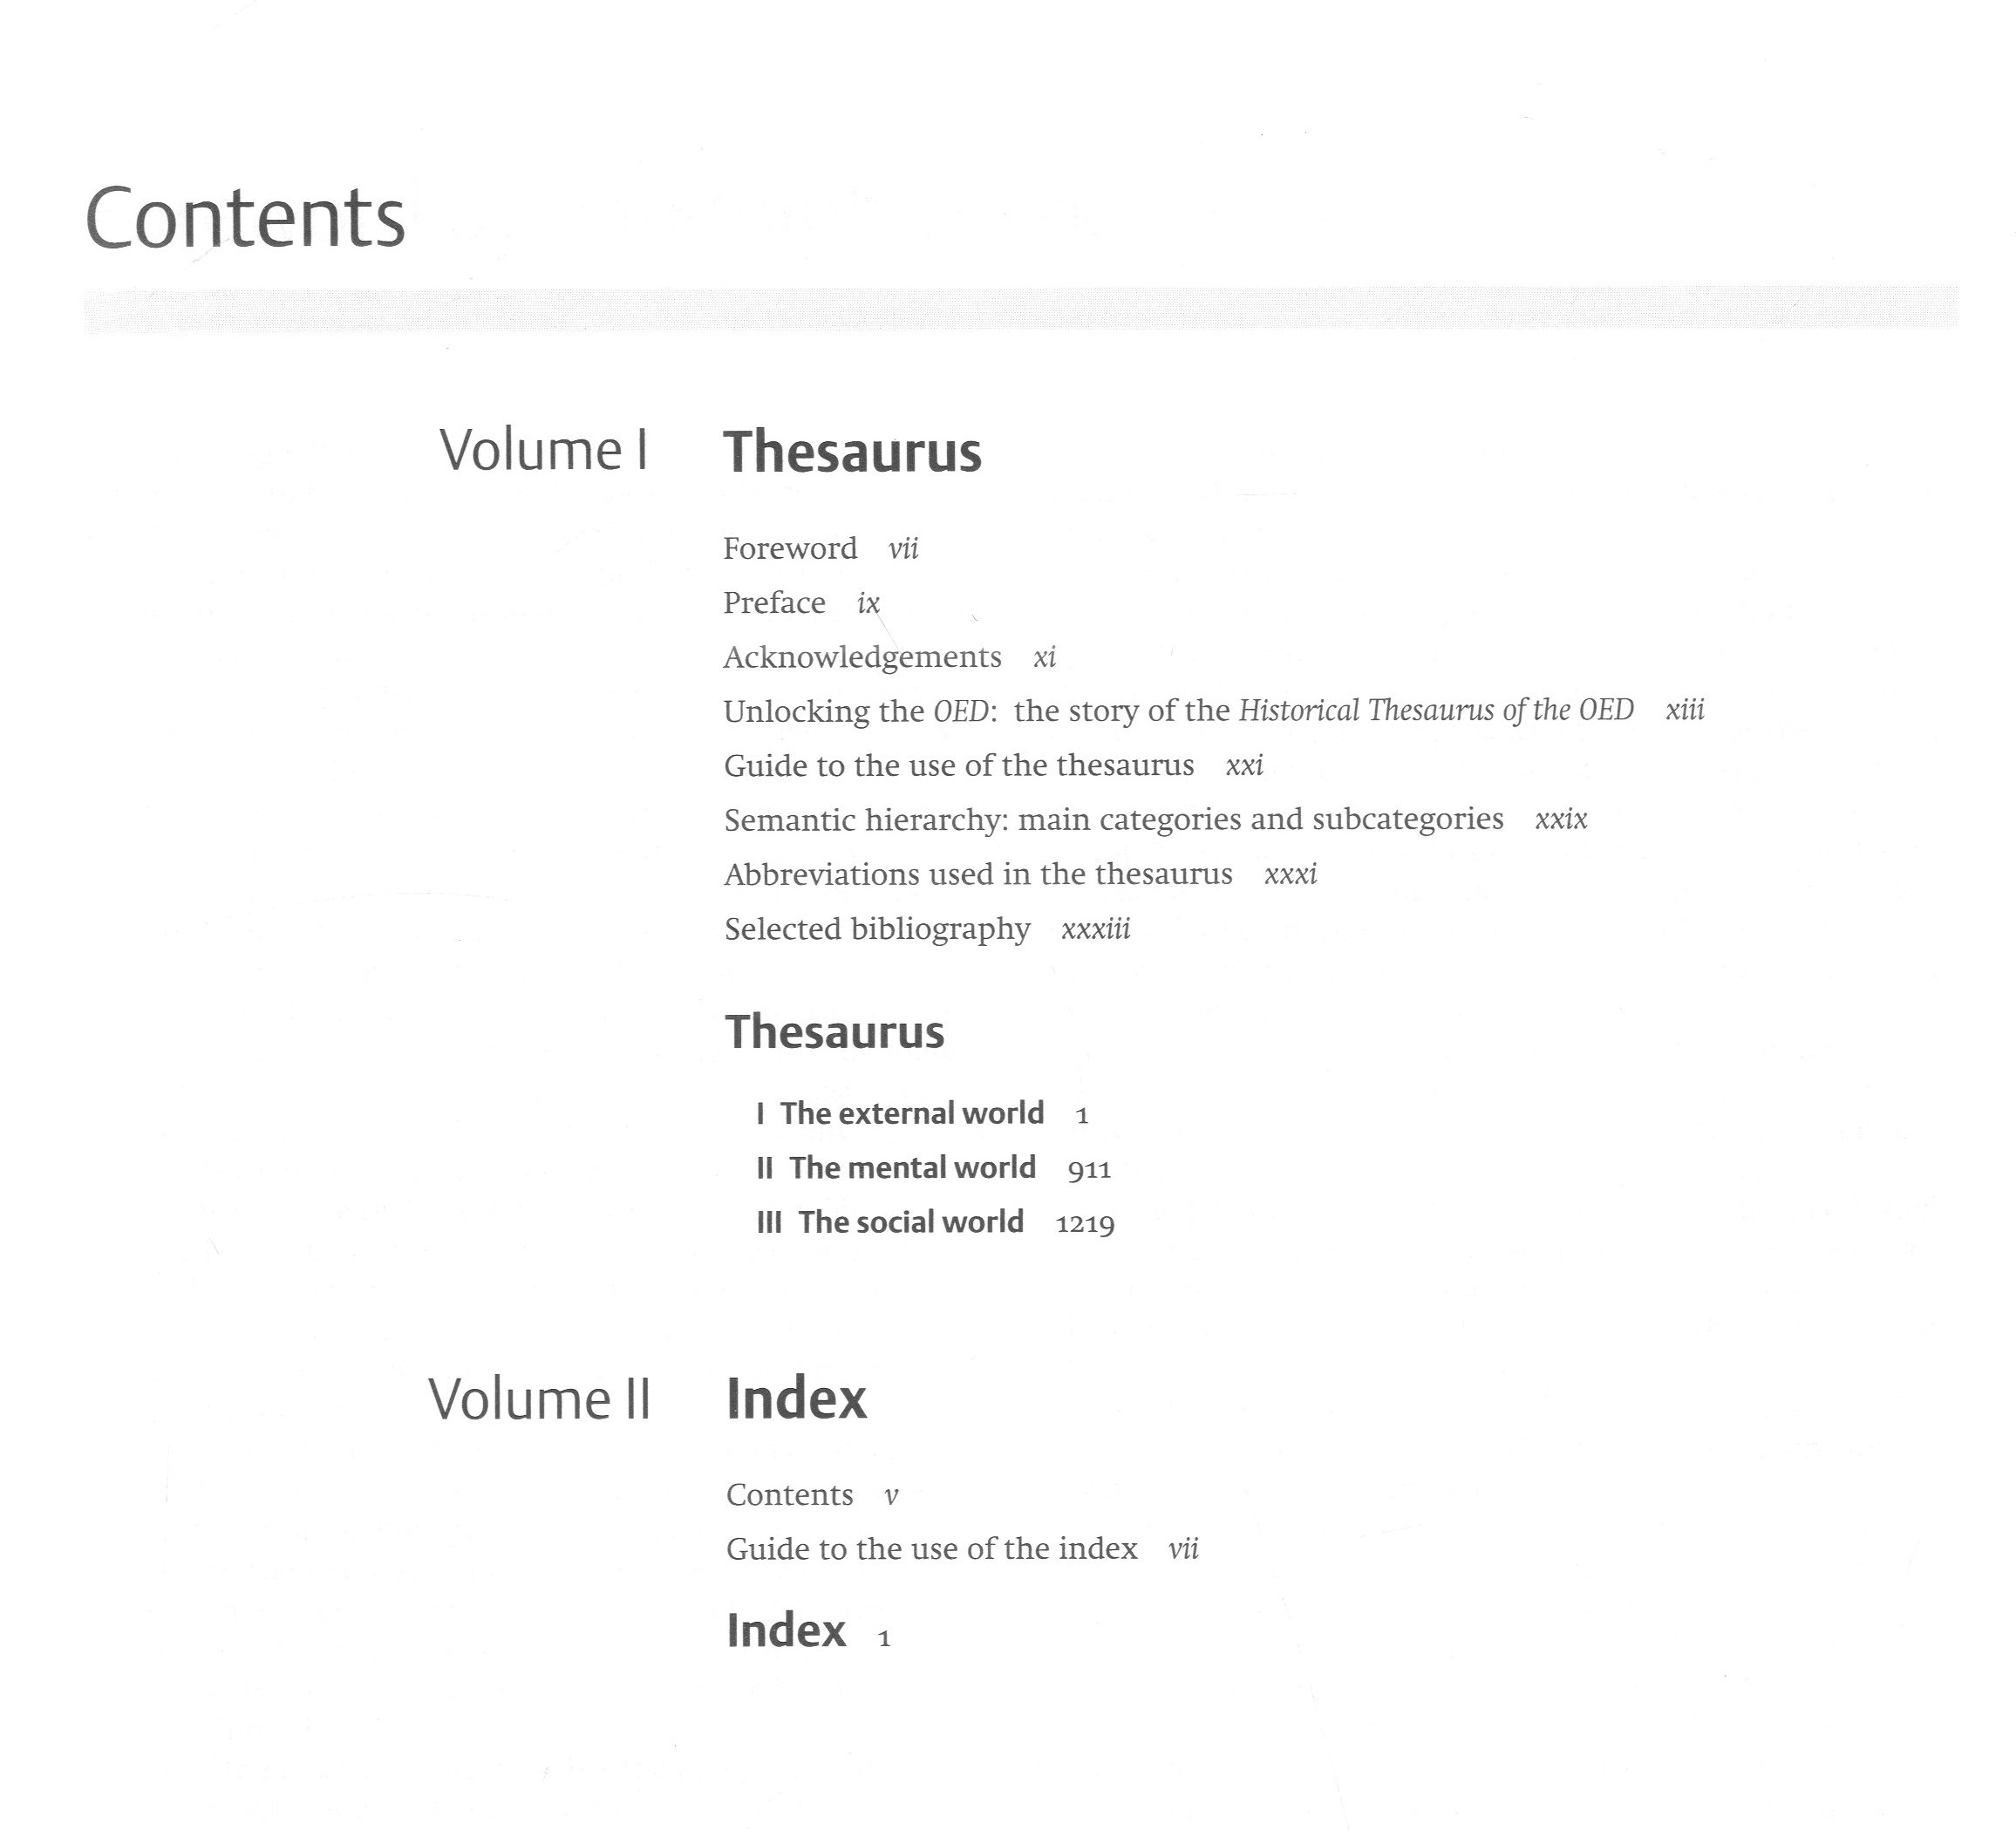
\includegraphics{Stolk_thes-content/fig/HTE-toc.jpg}
		}
	}
	\caption[]{\label{fig:Stolk_thes-content:HTE-toc} The table of contents from \textit{HTE1} (vol.1, p.v).}
\end{figure} 


%This chapter draws from two types of sources in order to provide an overview of the information found in thesauri: (1) existing historical language thesauri and (2) publications and handbooks on both thesauri and lexicography in general. The three main logical parts of thesauri that are, thus, distinguished are: (1) the topical system, which is a hierarchy of semantic concepts; (2) lexical senses, which are words or phrases in a specific sense, positioned within the overarching topical system; and, optionally, (3) relations of synonymy, indicated through groupings of lexical senses.

In order to provide an overview of the information found in historical language thesauri, the chapter draws from two main types of sources. The first, and most important kind of source, is the historical language thesauri themselves. This chapter analyses thesauri of Scots and English, specifically. Both their content proper and their introductions provide valuable insights into the main components found within historical language thesauri. The second group of sources is formed by publications and handbooks on both thesauri and lexicography in general. These secondary sources impart a broader understanding of the scope and context of historical language thesauri on the one hand and, on the other, delve more deeply into the semantics of some of the elements found in these thesauri. %Lastly, academic reviews and research employing thesauri are used in order to establish which aspects of the existing historical language thesauri are deemed an asset, and which were found wanting or absent.
%The chapter presents the findings from the analysis of these sources, which should provide the reader with a more transparent narrative than through a discussion and positioning of each source separately.

The remainder of the chapter is laid out as follows. Section \ref{sect:Stolk_thes-content:HLTs} lists available editions of historical language thesauri of Scots and English. Subsequently, section \ref{sect:Stolk_thes-content:MainComponents} identifies the main components found in these historical language thesauri. The traditional lexicographic perspective, which is based on the presentation of thesauri, is argued to be less suitable for electronic editions than for paper ones and is therefore supplanted by an alternative division into components --- one based on the knowledge that presentations convey. 
%Each of the components identified is, along with its constituents, treated in a separate section. 
The three components identified thus, treated separately in sections \ref{sect:Stolk_thes-content:TopicalSystem}--\ref{sect:Stolk_thes-content:Synonymy}, are: (1) the topical system, which is a hierarchy of semantic concepts; (2) lexical senses, which are words or phrases in a specific sense, positioned within the overarching topical system; and (3) relations of synonymy, indicated through groupings of lexical senses. 
%Before the conclusion of this chapter, two constituents that are found across these main components, namely cross-references and editorial commentaries, are discussed in section \ref{sect:Stolk_thes-content:CommonConstituents}. %sections \ref{sect:Stolk_thes-content:CrossReferences} and \ref{sect:Stolk_thes-content:EditorialCommentaries}, respectively.
Section \ref{sect:Stolk_thes-content:CommonConstituents} discusses two constituents that are found across these main components, namely cross-references and editorial commentaries. Before the conclusion of the chapter, section \ref{sect:Stolk_thes-content:RelatedResources} provides an overview of resources that, content-wise, have much in common with historical language thesauri.


 

\section{Historical language thesauri}
\label{sect:Stolk_thes-content:HLTs}

At the time of writing, historical language thesauri are relatively rare.\footnote{Hartmann, \textit{Encyclopedia of Language and Linguistics}, 2nd edn, s.v. `Thesauruses'; Kay and Alexander, `Diachronic and Synchronic Thesauruses'.} This chapter discusses eight thesauri that cover historical variants of English and Scots, in their various published forms. Only one encompasses the full history of the language which it covers; the others focus on a specific period and, often, a selected domain. A brief overview of the eight thesauri, and the various editions they are available in, is presented below (in order of publication date); \hyperref[Appendix1.A]{Appendix 1.A} contains illustrative images of each thesaurus.

\bigskip
\noindent
\textbf{\textit{A Dictionary of Selected Synonyms of the Principal Indo-European Languages (DSSPIEL)}}\\
\textit{DSSPIEL} captures synonyms from a number of Indo-European languages. It includes Greek, Latin, Spanish, Polish, and Russian, amongst others, but also historical forms of languages, such as Old, Middle, and Modern High German (or, as it is known in this thesaurus, New High German). This multi-lingual thesaurus appeared in print in 1949. 

\bigskip
\noindent
\textbf{\textit{The Scots Thesaurus (ScT)}}\\
\textit{ScT} captures the Lowland Scots lexis available throughout history, from its twelfth-century beginnings to the present. 
%This thesaurus categorizes its lexis but does not indicate synonymy.
It appeared in print in 1990.

\bigskip
\noindent
\textbf{\textit{A Shakespeare Thesaurus (ShT)}}\\
\textit{ShT} captures the vocabulary employed by the English poet and playwright William Shakespeare (1564-1616) throughout his works. 
%This thesaurus categorizes its lexis but does not indicate synonymy.
It appeared in print in 1993.

\bigskip
\noindent
\textbf{\textit{A Thesaurus of Old English (TOE)}}\\
\textit{TOE} captures the lexis of Old English, the variant of English spoken between roughly 500 and 1100 by the Anglo-Saxons. This thesaurus groups synonyms and provides insight into their distribution in the surviving Old English texts. Table \ref{table:Stolk_thes-content:editions-TOE} lists four editions of \textit{TOE} that can be distinguished.

\begin{table}[h!]
    \centering
    \small
    \begin{tabular}{llp{2.8in}c}
    \toprule
        \textbf{Edition} & \textbf{Type} & \textbf{Description} & \textbf{Published} \\ 
    \midrule
    \textit{TOE1} & print & the first publication of the thesaurus & 1995 \\
    \textit{TOE2} & print & a new impression, containing minor corrections and additions & 2000 \\
    \textit{TOE3} & electronic & a website containing further corrections, based on new knowledge that stemmed ``largely from completed sections of the Toronto Dictionary of Old English'' \footnote{Kay, `\textit{A Thesaurus of Old English} Online'%, \textit{Old English Newsletter} 38.3 (2005), 36–40.
    } --- \textit{no longer available} & 2005 \\
    \textit{TOE4} & electronic & a visual overhaul and relocation of the website of \textit{TOE3} [under rolling revision] & 2015 \\
    \midrule
    \end{tabular}
    \caption[]{\label{table:Stolk_thes-content:editions-TOE}Editions of \textit{TOE}}
\end{table}

\bigskip
\noindent
\textbf{\textit{Love, Sex and Marriage (LSM)}}\\
\textit{LSM} captures the English lexis available for love, sex, and marriage throughout the entire history of English. This thesaurus groups synonyms and provides insight into their use in time and place. \textit{LSM} appeared in print in 1999.

\bigskip
\noindent
\textbf{\textit{Historical Thesaurus of English (HTE)}}\\
\textit{HTE} captures the English lexis that has existed throughout its 1300-year history, from Old English up to Modern English. This thesaurus groups synonyms and provides insight into their use in time and place. Table \ref{table:Stolk_thes-content:editions-HTE} lists three editions of \textit{HTE} that can be distinguished.

\begin{table}[h!]
    \centering
    \small
    \begin{tabular}{llp{2.8in}c}
    \toprule
        \textbf{Edition} & \textbf{Type} & \textbf{Description} & \textbf{Published} \\ 
    \midrule
    \textit{HTE1} & print & the first publication of the thesaurus & 2009 \\
    \textit{HTE2} & electronic & a digital edition incorporated into \textit{OED Online} [under rolling revision] & 2010 \\
    \textit{HTE3} & electronic & a stand-alone website made freely available on the fiftieth anniversary of the founding of the thesaurus project [under rolling revision] & 2014 \\
    \midrule
    \end{tabular}
    \caption[]{\label{table:Stolk_thes-content:editions-HTE}Editions of \textit{HTE}}
\end{table}


\bigskip
\noindent
\textbf{\textit{Historical Thesaurus of Scots (HTS)}}\\
\textit{HTS} will capture the vocabulary of Scots throughout its known history. At the time of writing, the thesaurus is still in its pilot phase and focuses on a few selected fields. The pilot version of this thesaurus was published online as a website in 2015.

\bigskip
\noindent
\textbf{\textit{The Bilingual Thesaurus of Everyday Life in Medieval England} (\textit{BTH})}\\
\textit{BTH} contains vocabulary of two languages in use in Medieval England, namely Anglo-French and Middle English, relating to everyday life. %: Building, Domestic Activities, Farming, Food preparation, Manufacture, Trade, and Travel by water. 
This thesaurus groups words and phrases considered synonymous (or possible translations, when dealing with terms from both languages covered) and includes dates of attestation. The thesaurus was published online as a website in 2019.


%\section{Content of historical language thesauri}
%\section{Scope}
\section{Main components}
\label{sect:Stolk_thes-content:MainComponents}


The content of historical language thesauri consists of a number of main components, each with its own constituents, and relations between these components. 
%\section{Main components of thesaurus content}
%\label{sect:Stolk_thes-content:MainComponents}
Werner Hüllen, in his thorough treatment of the history of Roget's \textit{Thesaurus}, distinguishes two main components of thesauri proper: their macrostructure and microstructure.\footnote{Hüllen, \textit{A History of Roget's} Thesaurus, pp. 278–84.} 
%\textit{: Origins, Development, and Design}% (Oxford, 2004)
This distinction is common in lexicography and applied more generally also to dictionaries.\footnote{Additionally, the entire structure of the publication, along with its introductory apparatus (Foreword, Preface, etc.), is referred to as the megastructure. See Svensén, \textit{A Handbook of Lexicography}, p. 379.} %: The Theory and Practice of Dictionary-Making} %(Cambridge, 2009)
The term \textit{macrostructure} denotes the arrangement of entries; \textit{microstructure} indicates the structure applied \textit{within} entries. Although this distinction can be applied to historical language thesauri, too, maintaining it is not without its drawbacks. 

Firstly, what an entry exactly is can differ from one thesaurus to the next due to differences in presentation. In \textit{LSM}, for instance, an entry consists of a short sense definition (i.e., the name of the category), followed by a list of English words and phrases that, historically, have had that meaning. 
%In \textit{Roget's}, for instance, an entry consists of groups of loose synonyms that are identified together by a single number.\footnote{W. Hüllen, \textit{A History of Roget's} Thesaurus\textit{: Origins, Development, and Design} (Oxford, 2004), pp. 337–47.} 
In \textit{ScT}, an entry is a word with one or more senses. Entries can thus range from multiple sets of synonyms to a single set of these, or even to a single word sense.\footnote{What constitutes an entry and which information is presented as part of an entry during the editorial process can influence the compilation of the lexicographic work (see, for instance, the practice of employing template entries as discussed in Atkins and Rundell, \textit{The Oxford Guide to Practical Lexicography}, pp. 123-8.} As a consequence, discussions based on macrostructure and microstructure forestall comparisons of thesauri based not on presentation but on what they convey: their informational content. The latter is with which this chapter is concerned.

Secondly, the thesaurus taxonomy can be part of both the macrostructure and microstructure. This is the case for \textit{TOE} and \textit{HTE}. Their entries, as presented in print editions, are groups of synonyms that further expand on, or specialize, the categories found in the overarching macrostructure.\footnote{Such fine-grained distinction in meaning between groupings causes the microstructure to be termed distinctive as opposed to cumulative (Kay and Alexander, `Diachronic and Synchronic Thesauruses', p. 370).} Rather than discussing the hierarchy in the macrostructure and microstructure separately, reviewers of the historical language thesauri tend to discuss the topical system in its entirety.\footnote{E.g., Coleman, Review of \textit{HTE1}; Diller, Review of \textit{HTE1}; Görlach, Review of \textit{TOE1}; Momma, Review of \textit{TOE2}.} Their choice to do so is unsurprising, since which categories of the taxonomy belong to the macrostructure and which to the microstructure can be rather obscure. That is to say, the categories and the items they contain are sometimes presented in a similar manner for both categories belonging to the macrostructure and those considered part of the microstructure. In \textit{TOE2}, for instance, categories found in both structures are presented in bold and are followed by Old English synonyms that express their meaning (see categories ``01 Earth, world'' and ``.As God's creation'' in Figure \ref{fig:1.A:TOE2:thesaurus} in \hyperref[Appendix1.A]{Appendix 1.A}). The sole distinguishing factor between categories in its macrostructure and microstructure here appears to be that which precedes the category name: a string of numbers, in the case of the macrostructure, or points.\footnote{This difference, concerning the identification of categories, is discussed further in section \ref{sect:Stolk_thes-content:categories-id}.}

Thirdly, the distinction does not carry over well into electronic environments. Digital editions of historical language thesauri are no longer bound by the limitations that applied to their printed counterparts. Information is dispersed, accessible through hyperlinks, and not presented in a strict sequence and a single visualisation. The electronic editions of \textit{TOE}, \textit{HTE}, and \textit{HTS} focus on another distinction instead: between categories and the words they contain. Their search engines allow users to search amongst the former or the latter. to a singe information proper is separated from its presentation --- a design principle that is prevalent in information sciences.\footnote{Separation of structure and presentation has been advised, for instance, for web pages through the HTML and CSS standards. See W3C, `HTML \& CSS'.}%, \textit{Web Design and Applications}. \url{http://www.w3.org/standards/webdesign/htmlcss}. %Accessed on August 3, 2016.

In light of the above, the traditional distinction between macrostructure and microstructure should be abandoned. Instead, thesaurus content demands an analysis through the main logical components identified in digital editions of historical language thesauri. Thus, there are three parts of thesauri:
(1) the topical system, which is a hierarchy of semantic concepts; (2) lexical senses, which are words or phrases in a specific sense, positioned within the overarching topical system; and (3) relations of synonymy, indicated through groupings of lexical senses.\footnote{The term \textit{lexical senses} corresponds with the notion of \textit{lexical unit} as defined by Alan Cruse: ``the  union of a single sense with a lexical form'' (\textit{Lexical Semantics}, p. 77). Although relations other than synonymy, such as metonymy and polysemy, may be discerned in thesauri, too, they are, with the exception of \textit{HTE2}, not captured explicitly in the thesauri analysed.}
% The first component is the hierarchy of categories that will be referred to as the topical system. The second one is the lexemes themselves -- or, to be more accurate, their senses. A lexical sense in a historical language thesaurus is located within the topical system and typically accompanied by additional information (e.g., its part of speech and usage features). 
These components, shown in Figure \ref{fig:Stolk_thes-content:Content-parts} (and its legend in Figure \ref{fig:Stolk_thes-content:legend}), are discussed separately in the next sections, starting with the topical system.


\begin{figure}[htbp]
	\framebox[\textwidth]{
		\scalebox{0.65}[0.65]{
		    % Graphic for TeX using PGF
% Title: C:\Users\Sander\Documents\Dropbox\PhD\images\Content-parts.dia
% Creator: Dia v0.97.2
% CreationDate: Mon Apr 03 08:42:47 2017
% For: Sander
% \usepackage{tikz}
% The following commands are not supported in PSTricks at present
% We define them conditionally, so when they are implemented,
% this pgf file will use them.
\ifx\du\undefined
  \newlength{\du}
\fi
\setlength{\du}{15\unitlength}
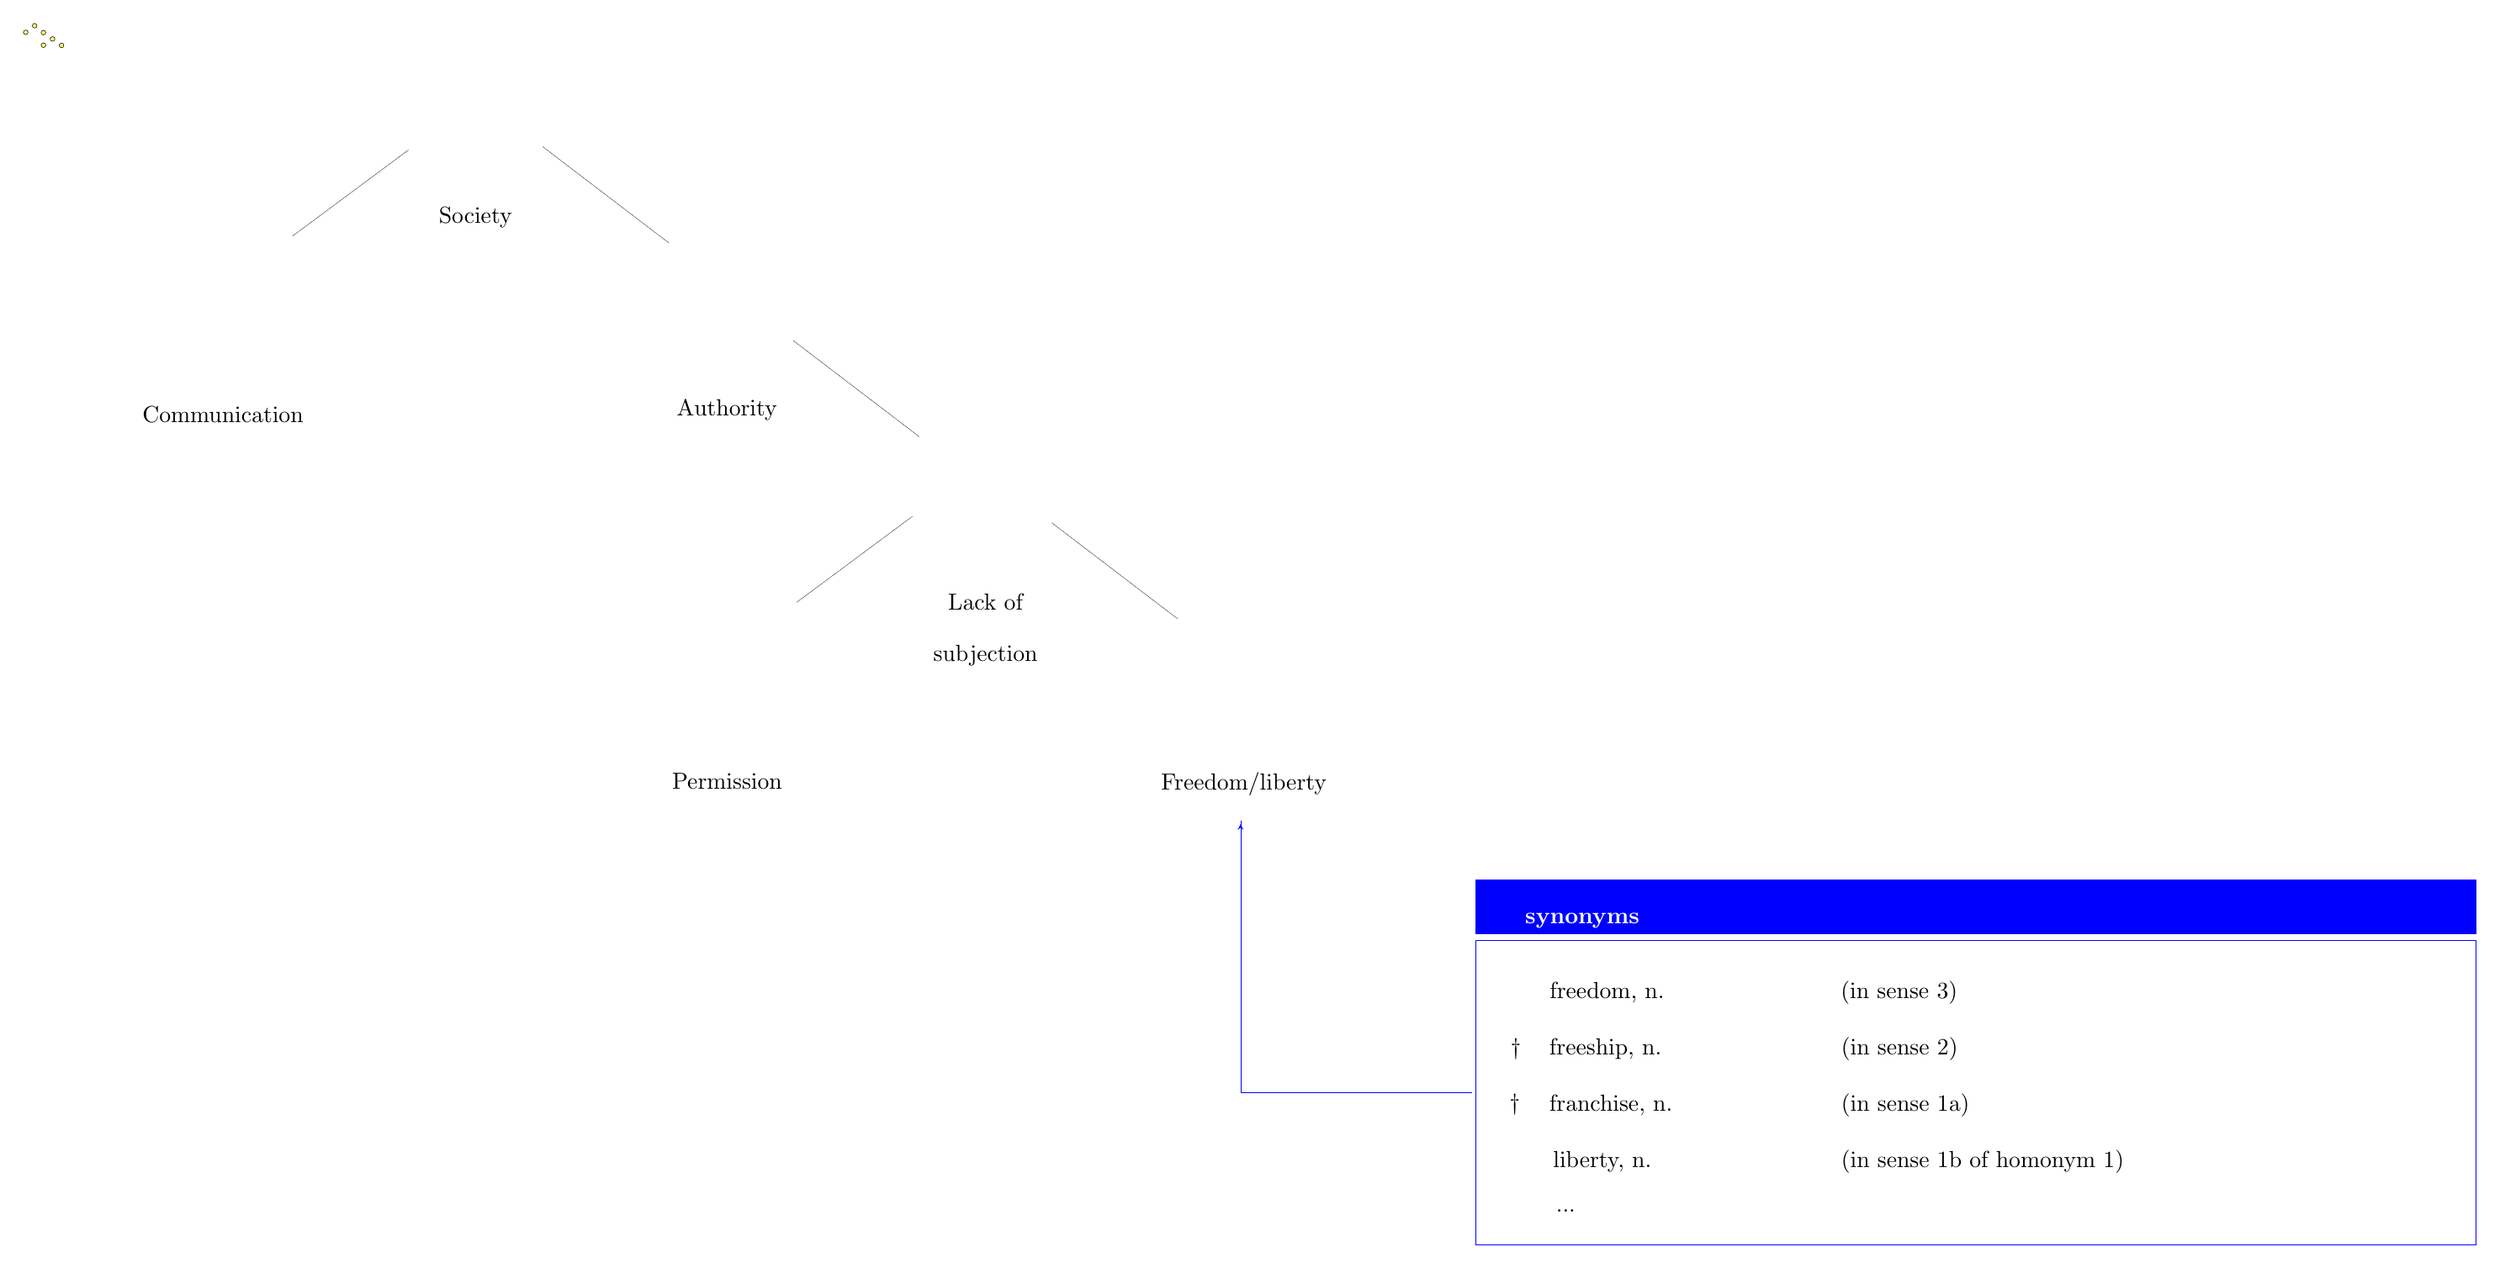
\begin{tikzpicture}
\pgftransformxscale{1.000000}
\pgftransformyscale{-1.000000}
\definecolor{dialinecolor}{rgb}{0.000000, 0.000000, 0.000000}
\pgfsetstrokecolor{dialinecolor}
\definecolor{dialinecolor}{rgb}{1.000000, 1.000000, 1.000000}
\pgfsetfillcolor{dialinecolor}
\pgfsetlinewidth{0.100000\du}
\pgfsetdash{}{0pt}
\pgfsetdash{}{0pt}
\pgfsetbuttcap
\pgfsetmiterjoin
\pgfsetlinewidth{0.100000\du}
\pgfsetbuttcap
\pgfsetmiterjoin
\pgfsetdash{}{0pt}
\definecolor{dialinecolor}{rgb}{1.000000, 0.984314, 0.435294}
\pgfsetfillcolor{dialinecolor}
\pgfpathellipse{\pgfpoint{14.600000\du}{6.900000\du}}{\pgfpoint{1.000000\du}{0\du}}{\pgfpoint{0\du}{1.000000\du}}
\pgfusepath{fill}
\definecolor{dialinecolor}{rgb}{0.000000, 0.000000, 0.000000}
\pgfsetstrokecolor{dialinecolor}
\pgfpathellipse{\pgfpoint{14.600000\du}{6.900000\du}}{\pgfpoint{1.000000\du}{0\du}}{\pgfpoint{0\du}{1.000000\du}}
\pgfusepath{stroke}
\pgfsetbuttcap
\pgfsetmiterjoin
\pgfsetdash{}{0pt}
\definecolor{dialinecolor}{rgb}{0.000000, 0.000000, 0.000000}
\pgfsetstrokecolor{dialinecolor}
\pgfpathellipse{\pgfpoint{14.600000\du}{6.900000\du}}{\pgfpoint{1.000000\du}{0\du}}{\pgfpoint{0\du}{1.000000\du}}
\pgfusepath{stroke}
\pgfsetlinewidth{0.100000\du}
\pgfsetdash{}{0pt}
\pgfsetdash{}{0pt}
\pgfsetmiterjoin
\definecolor{dialinecolor}{rgb}{1.000000, 1.000000, 1.000000}
\pgfsetfillcolor{dialinecolor}
% right-hand side of synonym box currently set to 37.100000
\fill (22.000000\du,13.850000\du)--(22.000000\du,18.450000\du)--(37.100000\du,18.450000\du)--(37.100000\du,13.850000\du)--cycle;
\definecolor{dialinecolor}{rgb}{0.000000, 0.000000, 1.000000}
\pgfsetstrokecolor{dialinecolor}
% right-hand side of synonym box currently set to 37.100000
\draw (22.000000\du,13.850000\du)--(22.000000\du,18.450000\du)--(37.100000\du,18.450000\du)--(37.100000\du,13.850000\du)--cycle;
% setfont left to latex
\definecolor{dialinecolor}{rgb}{0.000000, 0.000000, 0.000000}
\pgfsetstrokecolor{dialinecolor}
\node[anchor=west] at (23.050000\du,17.200000\du){liberty, n.};
% setfont left to latex
\definecolor{dialinecolor}{rgb}{0.000000, 0.000000, 0.000000}
\pgfsetstrokecolor{dialinecolor}
\node[anchor=west] at (23.000000\du,14.650000\du){freedom, n.};
\pgfsetlinewidth{0.100000\du}
\pgfsetdash{}{0pt}
\pgfsetdash{}{0pt}
\pgfsetmiterjoin
\pgfsetbuttcap
{
\definecolor{dialinecolor}{rgb}{0.000000, 0.000000, 1.000000}
\pgfsetfillcolor{dialinecolor}
% was here!!!
\pgfsetarrowsend{stealth}
{\pgfsetcornersarced{\pgfpoint{0.000000\du}{0.000000\du}}\definecolor{dialinecolor}{rgb}{0.000000, 0.000000, 1.000000}
\pgfsetstrokecolor{dialinecolor}
\draw (21.949713\du,16.150000\du)--(18.450000\du,16.150000\du)--(18.450000\du,12.100000\du)--(18.450000\du,12.100000\du);
}}
\definecolor{dialinecolor}{rgb}{1.000000, 1.000000, 1.000000}
\pgfsetfillcolor{dialinecolor}
\fill (16.050000\du,13.805000\du)--(16.050000\du,14.550000\du)--(16.050000\du,14.550000\du)--(16.050000\du,13.805000\du)--cycle;
% setfont left to latex
\definecolor{dialinecolor}{rgb}{0.000000, 0.000000, 0.000000}
\pgfsetstrokecolor{dialinecolor}
\node at (16.050000\du,14.400000\du){};
\definecolor{dialinecolor}{rgb}{1.000000, 1.000000, 1.000000}
\pgfsetfillcolor{dialinecolor}
\fill (12.726250\du,8.155000\du)--(12.726250\du,9.700000\du)--(16.473750\du,9.700000\du)--(16.473750\du,8.155000\du)--cycle;
% setfont left to latex
\definecolor{dialinecolor}{rgb}{0.000000, 0.000000, 0.000000}
\pgfsetstrokecolor{dialinecolor}
\node at (14.600000\du,8.750000\du){Lack of };
% setfont left to latex
\definecolor{dialinecolor}{rgb}{0.000000, 0.000000, 0.000000}
\pgfsetstrokecolor{dialinecolor}
\node at (14.600000\du,9.550000\du){subjection};
\pgfsetlinewidth{0.100000\du}
\pgfsetdash{}{0pt}
\pgfsetdash{}{0pt}
\pgfsetbuttcap
\pgfsetmiterjoin
\pgfsetlinewidth{0.100000\du}
\pgfsetbuttcap
\pgfsetmiterjoin
\pgfsetdash{}{0pt}
\definecolor{dialinecolor}{rgb}{1.000000, 0.984314, 0.435294}
\pgfsetfillcolor{dialinecolor}
\pgfpathellipse{\pgfpoint{10.695000\du}{4.150000\du}}{\pgfpoint{1.000000\du}{0\du}}{\pgfpoint{0\du}{1.000000\du}}
\pgfusepath{fill}
\definecolor{dialinecolor}{rgb}{0.000000, 0.000000, 0.000000}
\pgfsetstrokecolor{dialinecolor}
\pgfpathellipse{\pgfpoint{10.695000\du}{4.150000\du}}{\pgfpoint{1.000000\du}{0\du}}{\pgfpoint{0\du}{1.000000\du}}
\pgfusepath{stroke}
\pgfsetbuttcap
\pgfsetmiterjoin
\pgfsetdash{}{0pt}
\definecolor{dialinecolor}{rgb}{0.000000, 0.000000, 0.000000}
\pgfsetstrokecolor{dialinecolor}
\pgfpathellipse{\pgfpoint{10.695000\du}{4.150000\du}}{\pgfpoint{1.000000\du}{0\du}}{\pgfpoint{0\du}{1.000000\du}}
\pgfusepath{stroke}
\pgfsetlinewidth{0.100000\du}
\pgfsetdash{}{0pt}
\pgfsetdash{}{0pt}
\pgfsetbuttcap
\pgfsetmiterjoin
\pgfsetlinewidth{0.100000\du}
\pgfsetbuttcap
\pgfsetmiterjoin
\pgfsetdash{}{0pt}
\definecolor{dialinecolor}{rgb}{1.000000, 0.984314, 0.435294}
\pgfsetfillcolor{dialinecolor}
\pgfpathellipse{\pgfpoint{6.940000\du}{1.200000\du}}{\pgfpoint{1.000000\du}{0\du}}{\pgfpoint{0\du}{1.000000\du}}
\pgfusepath{fill}
\definecolor{dialinecolor}{rgb}{0.000000, 0.000000, 0.000000}
\pgfsetstrokecolor{dialinecolor}
\pgfpathellipse{\pgfpoint{6.940000\du}{1.200000\du}}{\pgfpoint{1.000000\du}{0\du}}{\pgfpoint{0\du}{1.000000\du}}
\pgfusepath{stroke}
\pgfsetbuttcap
\pgfsetmiterjoin
\pgfsetdash{}{0pt}
\definecolor{dialinecolor}{rgb}{0.000000, 0.000000, 0.000000}
\pgfsetstrokecolor{dialinecolor}
\pgfpathellipse{\pgfpoint{6.940000\du}{1.200000\du}}{\pgfpoint{1.000000\du}{0\du}}{\pgfpoint{0\du}{1.000000\du}}
\pgfusepath{stroke}
\definecolor{dialinecolor}{rgb}{1.000000, 1.000000, 1.000000}
\pgfsetfillcolor{dialinecolor}
\fill (8.991250\du,5.250000\du)--(8.991250\du,5.995000\du)--(12.398750\du,5.995000\du)--(12.398750\du,5.250000\du)--cycle;
% setfont left to latex
\definecolor{dialinecolor}{rgb}{0.000000, 0.000000, 0.000000}
\pgfsetstrokecolor{dialinecolor}
\node at (10.695000\du,5.845000\du){Authority};
\definecolor{dialinecolor}{rgb}{1.000000, 1.000000, 1.000000}
\pgfsetfillcolor{dialinecolor}
\fill (5.570000\du,2.350000\du)--(5.570000\du,3.095000\du)--(8.227500\du,3.095000\du)--(8.227500\du,2.350000\du)--cycle;
% setfont left to latex
\definecolor{dialinecolor}{rgb}{0.000000, 0.000000, 0.000000}
\pgfsetstrokecolor{dialinecolor}
\node at (6.898750\du,2.945000\du){Society};
\pgfsetlinewidth{0.100000\du}
\pgfsetdash{}{0pt}
\pgfsetdash{}{0pt}
\pgfsetbuttcap
{
\definecolor{dialinecolor}{rgb}{0.000000, 0.000000, 0.000000}
\pgfsetfillcolor{dialinecolor}
% was here!!!
\definecolor{dialinecolor}{rgb}{0.000000, 0.000000, 0.000000}
\pgfsetstrokecolor{dialinecolor}
\draw (13.600000\du,6.250000\du)--(11.700000\du,4.800000\du);
}
\pgfsetlinewidth{0.100000\du}
\pgfsetdash{}{0pt}
\pgfsetdash{}{0pt}
\pgfsetbuttcap
{
\definecolor{dialinecolor}{rgb}{0.000000, 0.000000, 0.000000}
\pgfsetfillcolor{dialinecolor}
% was here!!!
\definecolor{dialinecolor}{rgb}{0.000000, 0.000000, 0.000000}
\pgfsetstrokecolor{dialinecolor}
\draw (9.815080\du,3.320080\du)--(7.915080\du,1.870080\du);
}
\pgfsetlinewidth{0.100000\du}
\pgfsetdash{}{0pt}
\pgfsetdash{}{0pt}
\pgfsetmiterjoin
\definecolor{dialinecolor}{rgb}{0.000000, 0.000000, 1.000000}
\pgfsetfillcolor{dialinecolor}
% right-hand side of synonym box currently set to 37.100000
\fill (21.997400\du,12.943200\du)--(21.997400\du,13.755370\du)--(37.100000\du,13.755370\du)--(37.100000\du,12.943200\du)--cycle;
\definecolor{dialinecolor}{rgb}{0.000000, 0.000000, 1.000000}
\pgfsetstrokecolor{dialinecolor}
% right-hand side of synonym box currently set to 37.100000
\draw (21.997400\du,12.943200\du)--(21.997400\du,13.755370\du)--(37.100000\du,13.755370\du)--(37.100000\du,12.943200\du)--cycle;
% setfont left to latex
\definecolor{dialinecolor}{rgb}{1.000000, 1.000000, 1.000000}
\pgfsetstrokecolor{dialinecolor}
\node[anchor=west,white] at (22.629800\du,13.562800\du){\textbf{\textcolor{white}{synonyms}}};
\pgfsetlinewidth{0.100000\du}
\pgfsetdash{}{0pt}
\pgfsetdash{}{0pt}
\pgfsetbuttcap
\pgfsetmiterjoin
\pgfsetlinewidth{0.100000\du}
\pgfsetbuttcap
\pgfsetmiterjoin
\pgfsetdash{}{0pt}
\definecolor{dialinecolor}{rgb}{1.000000, 0.984314, 0.435294}
\pgfsetfillcolor{dialinecolor}
\pgfpathellipse{\pgfpoint{18.500000\du}{9.650000\du}}{\pgfpoint{1.000000\du}{0\du}}{\pgfpoint{0\du}{1.000000\du}}
\pgfusepath{fill}
\definecolor{dialinecolor}{rgb}{0.000000, 0.000000, 0.000000}
\pgfsetstrokecolor{dialinecolor}
\pgfpathellipse{\pgfpoint{18.500000\du}{9.650000\du}}{\pgfpoint{1.000000\du}{0\du}}{\pgfpoint{0\du}{1.000000\du}}
\pgfusepath{stroke}
\pgfsetbuttcap
\pgfsetmiterjoin
\pgfsetdash{}{0pt}
\definecolor{dialinecolor}{rgb}{0.000000, 0.000000, 0.000000}
\pgfsetstrokecolor{dialinecolor}
\pgfpathellipse{\pgfpoint{18.500000\du}{9.650000\du}}{\pgfpoint{1.000000\du}{0\du}}{\pgfpoint{0\du}{1.000000\du}}
\pgfusepath{stroke}
\definecolor{dialinecolor}{rgb}{1.000000, 1.000000, 1.000000}
\pgfsetfillcolor{dialinecolor}
\fill (15.603750\du,10.905000\du)--(15.603750\du,11.650000\du)--(21.396250\du,11.650000\du)--(21.396250\du,10.905000\du)--cycle;
% setfont left to latex
\definecolor{dialinecolor}{rgb}{0.000000, 0.000000, 0.000000}
\pgfsetstrokecolor{dialinecolor}
\node at (18.500000\du,11.500000\du){Freedom/liberty};
\pgfsetlinewidth{0.100000\du}
\pgfsetdash{}{0pt}
\pgfsetdash{}{0pt}
\pgfsetbuttcap
{
\definecolor{dialinecolor}{rgb}{0.000000, 0.000000, 0.000000}
\pgfsetfillcolor{dialinecolor}
% was here!!!
\definecolor{dialinecolor}{rgb}{0.000000, 0.000000, 0.000000}
\pgfsetstrokecolor{dialinecolor}
\draw (17.500000\du,9.000000\du)--(15.600000\du,7.550000\du);
}
% setfont left to latex
\definecolor{dialinecolor}{rgb}{0.000000, 0.000000, 0.000000}
\pgfsetstrokecolor{dialinecolor}
\node[anchor=west] at (22.995000\du,15.495000\du){freeship, n.};
% setfont left to latex
\definecolor{dialinecolor}{rgb}{0.000000, 0.000000, 0.000000}
\pgfsetstrokecolor{dialinecolor}
\node[anchor=west] at (22.995000\du,16.345000\du){franchise, n.};
% setfont left to latex
\definecolor{dialinecolor}{rgb}{0.000000, 0.000000, 0.000000}
\pgfsetstrokecolor{dialinecolor}
\node[anchor=west] at (23.095000\du,17.945000\du){...};
% setfont left to latex
\definecolor{dialinecolor}{rgb}{0.000000, 0.000000, 0.000000}
\pgfsetstrokecolor{dialinecolor}
\node[anchor=west] at (27.395000\du,14.645000\du){(in sense 3)};
\pgfsetlinewidth{0.100000\du}
\pgfsetdash{}{0pt}
\pgfsetdash{}{0pt}
\pgfsetbuttcap
{
\definecolor{dialinecolor}{rgb}{0.000000, 0.000000, 0.000000}
\pgfsetfillcolor{dialinecolor}
% was here!!!
\definecolor{dialinecolor}{rgb}{0.000000, 0.000000, 0.000000}
\pgfsetstrokecolor{dialinecolor}
\draw (13.500000\du,7.450000\du)--(11.750000\du,8.750000\du);
}
\pgfsetlinewidth{0.100000\du}
\pgfsetdash{}{0pt}
\pgfsetdash{}{0pt}
\pgfsetbuttcap
\pgfsetmiterjoin
\pgfsetlinewidth{0.100000\du}
\pgfsetbuttcap
\pgfsetmiterjoin
\pgfsetdash{}{0pt}
\definecolor{dialinecolor}{rgb}{1.000000, 0.984314, 0.435294}
\pgfsetfillcolor{dialinecolor}
\pgfpathellipse{\pgfpoint{10.715080\du}{9.570080\du}}{\pgfpoint{1.000000\du}{0\du}}{\pgfpoint{0\du}{1.000000\du}}
\pgfusepath{fill}
\definecolor{dialinecolor}{rgb}{0.000000, 0.000000, 0.000000}
\pgfsetstrokecolor{dialinecolor}
\pgfpathellipse{\pgfpoint{10.715080\du}{9.570080\du}}{\pgfpoint{1.000000\du}{0\du}}{\pgfpoint{0\du}{1.000000\du}}
\pgfusepath{stroke}
\pgfsetbuttcap
\pgfsetmiterjoin
\pgfsetdash{}{0pt}
\definecolor{dialinecolor}{rgb}{0.000000, 0.000000, 0.000000}
\pgfsetstrokecolor{dialinecolor}
\pgfpathellipse{\pgfpoint{10.715080\du}{9.570080\du}}{\pgfpoint{1.000000\du}{0\du}}{\pgfpoint{0\du}{1.000000\du}}
\pgfusepath{stroke}
\definecolor{dialinecolor}{rgb}{1.000000, 1.000000, 1.000000}
\pgfsetfillcolor{dialinecolor}
\fill (8.708750\du,10.855000\du)--(8.708750\du,11.600000\du)--(12.691250\du,11.600000\du)--(12.691250\du,10.855000\du)--cycle;
% setfont left to latex
\definecolor{dialinecolor}{rgb}{0.000000, 0.000000, 0.000000}
\pgfsetstrokecolor{dialinecolor}
\node at (10.700000\du,11.450000\du){Permission};
\pgfsetlinewidth{0.100000\du}
\pgfsetdash{}{0pt}
\pgfsetdash{}{0pt}
\pgfsetbuttcap
{
\definecolor{dialinecolor}{rgb}{0.000000, 0.000000, 0.000000}
\pgfsetfillcolor{dialinecolor}
% was here!!!
\definecolor{dialinecolor}{rgb}{0.000000, 0.000000, 0.000000}
\pgfsetstrokecolor{dialinecolor}
\draw (5.886250\du,1.919950\du)--(4.136250\du,3.219950\du);
}
\pgfsetlinewidth{0.100000\du}
\pgfsetdash{}{0pt}
\pgfsetdash{}{0pt}
\pgfsetbuttcap
\pgfsetmiterjoin
\pgfsetlinewidth{0.100000\du}
\pgfsetbuttcap
\pgfsetmiterjoin
\pgfsetdash{}{0pt}
\definecolor{dialinecolor}{rgb}{1.000000, 0.984314, 0.435294}
\pgfsetfillcolor{dialinecolor}
\pgfpathellipse{\pgfpoint{3.101330\du}{4.040030\du}}{\pgfpoint{1.000000\du}{0\du}}{\pgfpoint{0\du}{1.000000\du}}
\pgfusepath{fill}
\definecolor{dialinecolor}{rgb}{0.000000, 0.000000, 0.000000}
\pgfsetstrokecolor{dialinecolor}
\pgfpathellipse{\pgfpoint{3.101330\du}{4.040030\du}}{\pgfpoint{1.000000\du}{0\du}}{\pgfpoint{0\du}{1.000000\du}}
\pgfusepath{stroke}
\pgfsetbuttcap
\pgfsetmiterjoin
\pgfsetdash{}{0pt}
\definecolor{dialinecolor}{rgb}{0.000000, 0.000000, 0.000000}
\pgfsetstrokecolor{dialinecolor}
\pgfpathellipse{\pgfpoint{3.101330\du}{4.040030\du}}{\pgfpoint{1.000000\du}{0\du}}{\pgfpoint{0\du}{1.000000\du}}
\pgfusepath{stroke}
\definecolor{dialinecolor}{rgb}{1.000000, 1.000000, 1.000000}
\pgfsetfillcolor{dialinecolor}
\fill (0.282500\du,5.324950\du)--(0.282500\du,6.069950\du)--(5.890000\du,6.069950\du)--(5.890000\du,5.324950\du)--cycle;
% setfont left to latex
\definecolor{dialinecolor}{rgb}{0.000000, 0.000000, 0.000000}
\pgfsetstrokecolor{dialinecolor}
\node at (3.086250\du,5.919950\du){Communication};
% setfont left to latex
\definecolor{dialinecolor}{rgb}{0.000000, 0.000000, 0.000000}
\pgfsetstrokecolor{dialinecolor}
\node[anchor=west] at (27.400000\du,15.500000\du){(in sense 2)};
% setfont left to latex
\definecolor{dialinecolor}{rgb}{0.000000, 0.000000, 0.000000}
\pgfsetstrokecolor{dialinecolor}
\node[anchor=west] at (27.400000\du,16.350000\du){(in sense 1a)};
% setfont left to latex
\definecolor{dialinecolor}{rgb}{0.000000, 0.000000, 0.000000}
\pgfsetstrokecolor{dialinecolor}
\node[anchor=west] at (27.400000\du,17.200000\du){(in sense 1b of homonym 1)};
% setfont left to latex
\definecolor{dialinecolor}{rgb}{0.000000, 0.000000, 0.000000}
\pgfsetstrokecolor{dialinecolor}
\node[anchor=west] at (22.410000\du,15.495000\du){$\dagger$};
% setfont left to latex
\definecolor{dialinecolor}{rgb}{0.000000, 0.000000, 0.000000}
\pgfsetstrokecolor{dialinecolor}
\node[anchor=west] at (22.395000\du,16.340000\du){$\dagger$};
\end{tikzpicture}

%            \includesvg[inkscapelatex=false,width=\textwidth]{Stolk_thes-content/fig/Content-parts.svg}
		}
	}
	\caption[]{\label{fig:Stolk_thes-content:Content-parts} Three logical components of a thesaurus, as found in \textit{HTE2}.}
\end{figure} 

\begin{figure}[htbp]
	\framebox[\textwidth]{
		\scalebox{0.65}[0.65]{
		    % Graphic for TeX using PGF
% Title: C:\Users\Sander\Documents\Dropbox\PhD\images\legend.dia
% Creator: Dia v0.97.2
% CreationDate: Wed Jan 02 16:12:26 2019
% For: Sander
% \usepackage{tikz}
% The following commands are not supported in PSTricks at present
% We define them conditionally, so when they are implemented,
% this pgf file will use them.
\ifx\du\undefined
  \newlength{\du}
\fi
\setlength{\du}{15\unitlength}
\begin{tikzpicture}
\pgftransformxscale{1.000000}
\pgftransformyscale{-1.000000}
\definecolor{dialinecolor}{rgb}{0.000000, 0.000000, 0.000000}
\pgfsetstrokecolor{dialinecolor}
\definecolor{dialinecolor}{rgb}{1.000000, 1.000000, 1.000000}
\pgfsetfillcolor{dialinecolor}
\pgfsetlinewidth{0.100000\du}
\pgfsetdash{}{0pt}
\pgfsetdash{}{0pt}
\pgfsetmiterjoin
\pgfsetbuttcap
{
\definecolor{dialinecolor}{rgb}{0.000000, 0.000000, 1.000000}
\pgfsetfillcolor{dialinecolor}
% was here!!!
\pgfsetarrowsend{stealth}
{\pgfsetcornersarced{\pgfpoint{0.000000\du}{0.000000\du}}\definecolor{dialinecolor}{rgb}{0.000000, 0.000000, 1.000000}
\pgfsetstrokecolor{dialinecolor}
\draw (2.050000\du,4.950000\du)--(1.195810\du,4.950000\du)--(1.195810\du,3.100000\du)--(1.195810\du,3.100000\du);
}}
\pgfsetlinewidth{0.100000\du}
\pgfsetdash{}{0pt}
\pgfsetdash{}{0pt}
\pgfsetbuttcap
\pgfsetmiterjoin
\pgfsetlinewidth{0.100000\du}
\pgfsetbuttcap
\pgfsetmiterjoin
\pgfsetdash{}{0pt}
\definecolor{dialinecolor}{rgb}{1.000000, 0.984314, 0.435294}
\pgfsetfillcolor{dialinecolor}
\pgfpathellipse{\pgfpoint{1.190000\du}{1.200000\du}}{\pgfpoint{1.000000\du}{0\du}}{\pgfpoint{0\du}{1.000000\du}}
\pgfusepath{fill}
\definecolor{dialinecolor}{rgb}{0.000000, 0.000000, 0.000000}
\pgfsetstrokecolor{dialinecolor}
\pgfpathellipse{\pgfpoint{1.190000\du}{1.200000\du}}{\pgfpoint{1.000000\du}{0\du}}{\pgfpoint{0\du}{1.000000\du}}
\pgfusepath{stroke}
\pgfsetbuttcap
\pgfsetmiterjoin
\pgfsetdash{}{0pt}
\definecolor{dialinecolor}{rgb}{0.000000, 0.000000, 0.000000}
\pgfsetstrokecolor{dialinecolor}
\pgfpathellipse{\pgfpoint{1.190000\du}{1.200000\du}}{\pgfpoint{1.000000\du}{0\du}}{\pgfpoint{0\du}{1.000000\du}}
\pgfusepath{stroke}
\definecolor{dialinecolor}{rgb}{1.000000, 1.000000, 1.000000}
\pgfsetfillcolor{dialinecolor}
\fill (3.898750\du,0.707500\du)--(3.898750\du,1.695000\du)--(8.493750\du,1.695000\du)--(8.493750\du,0.707500\du)--cycle;
% setfont left to latex
\definecolor{dialinecolor}{rgb}{0.000000, 0.000000, 0.000000}
\pgfsetstrokecolor{dialinecolor}
\node[anchor=west] at (3.898750\du,1.495000\du){A category};
\definecolor{dialinecolor}{rgb}{1.000000, 1.000000, 1.000000}
\pgfsetfillcolor{dialinecolor}
\fill (3.845000\du,3.550000\du)--(3.845000\du,4.537500\du)--(14.302500\du,4.537500\du)--(14.302500\du,3.550000\du)--cycle;
% setfont left to latex
\definecolor{dialinecolor}{rgb}{0.000000, 0.000000, 0.000000}
\pgfsetstrokecolor{dialinecolor}
\node[anchor=west] at (3.845000\du,4.337500\du){Categorization of senses};
\pgfsetlinewidth{0.100000\du}
\pgfsetdash{}{0pt}
\pgfsetdash{}{0pt}
\pgfsetmiterjoin
\definecolor{dialinecolor}{rgb}{1.000000, 1.000000, 1.000000}
\pgfsetfillcolor{dialinecolor}
\fill (17.895000\du,0.300000\du)--(17.895000\du,2.000000\du)--(19.800000\du,2.000000\du)--(19.800000\du,0.300000\du)--cycle;
\definecolor{dialinecolor}{rgb}{0.000000, 0.000000, 1.000000}
\pgfsetstrokecolor{dialinecolor}
\draw (17.895000\du,0.300000\du)--(17.895000\du,2.000000\du)--(19.800000\du,2.000000\du)--(19.800000\du,0.300000\du)--cycle;
\definecolor{dialinecolor}{rgb}{1.000000, 1.000000, 1.000000}
\pgfsetfillcolor{dialinecolor}
\fill (21.245000\du,0.600000\du)--(21.245000\du,1.587500\du)--(27.605000\du,1.587500\du)--(27.605000\du,0.600000\du)--cycle;
% setfont left to latex
\definecolor{dialinecolor}{rgb}{0.000000, 0.000000, 0.000000}
\pgfsetstrokecolor{dialinecolor}
\node[anchor=west] at (21.245000\du,1.387500\du){A list of senses};
\pgfsetlinewidth{0.100000\du}
\pgfsetdash{}{0pt}
\pgfsetdash{}{0pt}
\pgfsetmiterjoin
\definecolor{dialinecolor}{rgb}{1.000000, 1.000000, 1.000000}
\pgfsetfillcolor{dialinecolor}
\fill (17.945000\du,3.250000\du)--(17.945000\du,4.950000\du)--(19.850000\du,4.950000\du)--(19.850000\du,3.250000\du)--cycle;
\definecolor{dialinecolor}{rgb}{0.000000, 0.000000, 1.000000}
\pgfsetstrokecolor{dialinecolor}
\draw (17.945000\du,3.250000\du)--(17.945000\du,4.950000\du)--(19.850000\du,4.950000\du)--(19.850000\du,3.250000\du)--cycle;
\pgfsetlinewidth{0.100000\du}
\pgfsetdash{}{0pt}
\pgfsetdash{}{0pt}
\pgfsetmiterjoin
\definecolor{dialinecolor}{rgb}{0.000000, 0.000000, 1.000000}
\pgfsetfillcolor{dialinecolor}
\fill (17.945000\du,3.250000\du)--(17.945000\du,3.800000\du)--(19.850000\du,3.800000\du)--(19.850000\du,3.250000\du)--cycle;
\definecolor{dialinecolor}{rgb}{0.000000, 0.000000, 1.000000}
\pgfsetstrokecolor{dialinecolor}
\draw (17.945000\du,3.250000\du)--(17.945000\du,3.800000\du)--(19.850000\du,3.800000\du)--(19.850000\du,3.250000\du)--cycle;
\definecolor{dialinecolor}{rgb}{1.000000, 1.000000, 1.000000}
\pgfsetfillcolor{dialinecolor}
\fill (21.245000\du,3.500000\du)--(21.245000\du,4.487500\du)--(33.237500\du,4.487500\du)--(33.237500\du,3.500000\du)--cycle;
% setfont left to latex
\definecolor{dialinecolor}{rgb}{0.000000, 0.000000, 0.000000}
\pgfsetstrokecolor{dialinecolor}
\node[anchor=west] at (21.245000\du,4.287500\du){A list of synonymous senses};
% setfont left to latex
\definecolor{dialinecolor}{rgb}{1.000000, 1.000000, 1.000000}
\pgfsetstrokecolor{dialinecolor}
\node[text=white] at (18.897500\du,3.650000\du){syno.};
\end{tikzpicture}

		}
	}
	\caption[]{\label{fig:Stolk_thes-content:legend} Legend.}
\end{figure} 

\section{Topical system}
\label{sect:Stolk_thes-content:TopicalSystem}
Dictionaries commonly employ an alphabetical ordering of their items. Thesauri, in contrast, organize their items according to their meaning through a topical structure. This overarching structure offers users generic meanings as a starting point, which branch out to meanings increasingly specific. Once users locate the meaning that they are interested in, they are presented with the words or phrases that express that meaning. This overarching system thus allows the thesaurus user to move from meaning to lexical item.

Topical systems in thesauri go by different names. Some thesauri, including \textit{LSM}, \textit{DSSPIEL}, and the paper editions of \textit{TOE}, refer to their overarching system as the classification system. Others, including \textit{HTE}, \textit{HTS}, \textit{ScT}, and the electronic edition of \textit{TOE}, position their topical structure as consisting of categories rather than classes, suggesting that their lexis has been categorized rather than classified. The terms \textit{classification} and \textit{categorization} are often thought to be synonymous and, as a result, ``literature on categorization is riddled with passages where the terms [..] are used indiscriminately''.\footnote{Jacob, `Classification and Categorization%: A Difference that Makes a Difference
', %\textit{Library Trends} 52.3 (2004), 515–40 (
p. 527.} In fact, the lack of distinction between \textit{class/classification} and \textit{category/categorization} can be found even in the entry on thesauri in the \textit{Encyclopedia of Language and Linguistics}, which contains a paragraph that speaks of categories in a classification system.\footnote{Hartmann, \textit{Encyclopedia of Language and Linguistics}%, 2nd edn, ed. K. Brown (Oxford, 2006)
, s.v. `Thesauruses'.} Nevertheless, there are differences worth noting.

Although classification and categorization are both means to group items, a classification provides the more rigid structure of the two.\footnote{Jacob, `Classification and Categorization', pp. 527–31.} The criteria for assigning items to a particular class are predetermined principles that ensure that the classes are mutually-exclusive and non-overlapping. In other words, an item can be assigned to only one specific branch in a classification system. Categories, by contrast, are formed based on context or perceived similarity rather than on predetermined principles. Their boundaries can be ``fuzzy'': some items may be considered better representative members of a category than others. Which items are assigned to a category and which ones are not therefore remains relatively flexible. Items that are categorized can belong to multiple groups, possibly even located in different branches of a hierarchy (if indeed categories are positioned within a hierarchy). The flexibility that categorization offers over classification is deemed ``essential'' for historical semantics in particular, according to the editors of \textit{HTE}.\footnote{\textit{HTE1}, p. xix. The fact that categorized items may differ in how well they reflect the grouping to which they are assigned is in line with what is known as the prototype theory, one of the more recent development in semantics. For an introduction to prototype theory, see Taylor, \textit{Encyclopedia of Language and Linguistics}, %2nd edn, ed. K. Brown (Oxford, 2006), 
s.v. `Prototype Semantics'.}  As a consequence, the terms \textit{category} and \textit{categorization} appear more suitable for historical language thesauri than \textit{class} and \textit{classification}. The former are therefore used in the remainder of this study.

The logic behind the topical system and its categories tends to be the ``central question'' for reviewers of thesauri.\footnote{Diller, Review of \textit{HTE1}, %\textit{Anglia} 128.2 (2010), 319–23 (
p. 321.} Manfred Görlach, for instance, has expressed his disappointment in finding in-depth discussion on this matter absent from \textit{TOE1}.\footnote{Görlach, Review of \textit{TOE1}, %\textit{Anglia} 116.3 (1998), 398–401 (
p. 398.} Görlach is not alone in criticizing the logic applied by editors (regardless of whether it is made explicit or not) and the resulting topical system.\footnote{See, for instance, Dance, Review of \textit{TOE1}, p. 312.} Such criticism did not catch the creators of the discussed thesauri unaware, however.\footnote{In the foreword or afterword of thesauri, editors typically convey their awareness that the fashioned topical system is only a best attempt and may well find disagreement with others (see \textit{DSSPIEL}, p. xiii; \textit{ShT}, p. viii; \textit{TOE2}, pp. xxxv–xxxvi; \textit{HTE1}, p. xix).} In fact, both creators and reviewers are conscious of the fact that, due to the subjective choices involved in constructing a topical system, it is unlikely that one can be formed that will satisfy every user.\footnote{For creators, see \textit{DSSPIEL}, p. xiii; \textit{ShT}, pp. viii–ix; \textit{TOE2}, pp. xxxv–xxxvi; \textit{HTE1}, p. xix; \textit{LSM}, p. 22.
For reviewers, see Diller, Review of \textit{HTE1}, p. 322; Peters, Review of \textit{LSM}, %\textit{Anglia} 120.3 (2003), 399–401 (
p. 400.} 

Andreas Fischer has explained the necessity of subjective choices in fashioning a thesaurus. The first reason, he contends, is that any fashioned topical system will be influenced by the ``[c]ultural conceptions and practices'' of its creators.\footnote{Fischer, `The Notional Structure of Thesauruses', %in \textit{Categorization in the History of English}, eds. C. J. Kay and J. J. Smith, \textit{Amsterdam Studies in the Theory and History of Linguistic Science} 4.261 (Amsterdam, 2004), pp. 41–58 (
p. 55.} The second reason is that ``human beings will see most concepts as belonging to several categories'' whereas thesauri typically limit the number of categories in order to achieve clarity and brevity.\footnote{Ibid., %in \textit{Categorization in the History of English}, eds. C. J. Kay and J. J. Smith, \textit{Amsterdam Studies in the Theory and History of Linguistic Science} 4.261 (Amsterdam, 2004), pp. 41–58 (
p. 55; see also Kay, `When Ignorance is Wisdom%: Some Day-to-Day Problems of Classification
', %in \textit{Categorization in the History of English}, eds. C. J. Kay and J. J. Smith, \textit{Amsterdam Studies in the Theory and History of Linguistic Science} 4.261 (Amsterdam, 2004), pp. 59–69 (
pp. 66–7.} 
Animals, as Fischer points out, can be allocated in the topical system of a thesaurus under categories of ``domestic or wild, or they can be distinguished according to what they eat''.\footnote{Fischer, `The Notional Structure of Thesauruses', p. 55.} 
Based on these premises, Hans-Jürgen Diller convincingly argues that ``[t]here is no one right classification [or categorization]; there are only more and less useful ones''.\footnote{Diller, Review of \textit{HTE1}, p. 322.} Of course, its usefulness will depend on the context in (or perhaps, rather, the purpose for) which the thesaurus and its topical structure is to be used. The following subsections address three aspects of topical systems: their structure and constituents (i.e., categories), co-ordination of these constituents, and their identification.

\subsection{Structure of topical systems and their categories}
%Topical systems in thesauri can vary widely, due to the lexis that they organize and due to inherently subjective choices in fashioning the overarching topical system. %Consequently, analysing which categories they contain exactly will not yield an understanding of historical language thesauri in general. A more sensible approach, taken in this section, is to review the characteristics, or structuring, of categories and of the topical systems they belong to as a whole.

The topical system of a thesaurus, which enables users to move from meaning to lexical items that convey that meaning, consists of categories that are placed in a hierarchical structure. This overarching structure, which is used to organize words and phrases, is not unlike the taxonomies of animals and plants created by the eighteenth-century biologist Carl Linnaeus (1707-1778) and later expanded by the zoologist Georges Cuvier (1769-1832).\footnote{Faria, `Georges Cuvier et le premier paradigme de la paléontologie'%, \textit{Revue de Paléobiologie} 32.2 (2013), 297–302
.} 
% NOTE TO SELF:
% The taxonomy has also been called ``the tree of life''. See BBC documentary by Attenborough (https://en.wikipedia.org/wiki/Charles_Darwin_and_the_Tree_of_Life), BBC news articles (http://www.bbc.com/news/science-environment-38585325) and the classification tree updated by scientists in an open source project (http://opentreeoflife.org , news article http://www.independent.co.uk/news/science/scientists-release-complete-tree-of-life-which-shows-how-23-million-species-are-related-10511433.html )
In these tree-like structures, the most generic or abstract concepts are used as roots, which branch out to concepts increasingly specific in meaning. The concepts lower down in the taxonomy are said to be subordinate to the more abstract ones they branch from.\footnote{%J. I. 
Saeed, \textit{Semantics}, %3rd edn, \textit{Introducing Linguistics 2} (Oxford, 2009), 
p. 68.} The ones from which they branch, in turn, are their superordinates (see Figure \ref{fig:Stolk_thes-content:HTE-ts-explained}).

\begin{figure}[h]
	\framebox[\textwidth]{
		\scalebox{0.65}[0.65]{
		    % Graphic for TeX using PGF
% Title: C:\Users\Sander\Documents\Dropbox\PhD\images\Content-part-TopicalSystem (explained).dia
% Creator: Dia v0.97.2
% CreationDate: Wed Apr 13 17:43:52 2022
% For: Sander
% \usepackage{tikz}
% The following commands are not supported in PSTricks at present
% We define them conditionally, so when they are implemented,
% this pgf file will use them.
\ifx\du\undefined
  \newlength{\du}
\fi
\setlength{\du}{15\unitlength}
\begin{tikzpicture}
\pgftransformxscale{1.000000}
\pgftransformyscale{-1.000000}
\definecolor{dialinecolor}{rgb}{0.000000, 0.000000, 0.000000}
\pgfsetstrokecolor{dialinecolor}
\definecolor{dialinecolor}{rgb}{1.000000, 1.000000, 1.000000}
\pgfsetfillcolor{dialinecolor}
\pgfsetlinewidth{0.100000\du}
\pgfsetdash{}{0pt}
\pgfsetdash{}{0pt}
\pgfsetbuttcap
\pgfsetmiterjoin
\pgfsetlinewidth{0.100000\du}
\pgfsetbuttcap
\pgfsetmiterjoin
\pgfsetdash{}{0pt}
\definecolor{dialinecolor}{rgb}{1.000000, 0.984314, 0.435294}
\pgfsetfillcolor{dialinecolor}
\pgfpathellipse{\pgfpoint{14.600000\du}{6.900000\du}}{\pgfpoint{1.000000\du}{0\du}}{\pgfpoint{0\du}{1.000000\du}}
\pgfusepath{fill}
\definecolor{dialinecolor}{rgb}{0.000000, 0.000000, 0.000000}
\pgfsetstrokecolor{dialinecolor}
\pgfpathellipse{\pgfpoint{14.600000\du}{6.900000\du}}{\pgfpoint{1.000000\du}{0\du}}{\pgfpoint{0\du}{1.000000\du}}
\pgfusepath{stroke}
\pgfsetbuttcap
\pgfsetmiterjoin
\pgfsetdash{}{0pt}
\definecolor{dialinecolor}{rgb}{0.000000, 0.000000, 0.000000}
\pgfsetstrokecolor{dialinecolor}
\pgfpathellipse{\pgfpoint{14.600000\du}{6.900000\du}}{\pgfpoint{1.000000\du}{0\du}}{\pgfpoint{0\du}{1.000000\du}}
\pgfusepath{stroke}
\definecolor{dialinecolor}{rgb}{1.000000, 1.000000, 1.000000}
\pgfsetfillcolor{dialinecolor}
\fill (16.050000\du,13.805000\du)--(16.050000\du,14.550000\du)--(16.050000\du,14.550000\du)--(16.050000\du,13.805000\du)--cycle;
% setfont left to latex
\definecolor{dialinecolor}{rgb}{0.000000, 0.000000, 0.000000}
\pgfsetstrokecolor{dialinecolor}
\node at (16.050000\du,14.400000\du){};
\definecolor{dialinecolor}{rgb}{1.000000, 1.000000, 1.000000}
\pgfsetfillcolor{dialinecolor}
\fill (12.726250\du,8.155000\du)--(12.726250\du,9.700000\du)--(16.473750\du,9.700000\du)--(16.473750\du,8.155000\du)--cycle;
% setfont left to latex
\definecolor{dialinecolor}{rgb}{0.000000, 0.000000, 0.000000}
\pgfsetstrokecolor{dialinecolor}
\node at (14.600000\du,8.750000\du){Lack of };
% setfont left to latex
\definecolor{dialinecolor}{rgb}{0.000000, 0.000000, 0.000000}
\pgfsetstrokecolor{dialinecolor}
\node at (14.600000\du,9.550000\du){subjection};
\pgfsetlinewidth{0.100000\du}
\pgfsetdash{}{0pt}
\pgfsetdash{}{0pt}
\pgfsetbuttcap
\pgfsetmiterjoin
\pgfsetlinewidth{0.100000\du}
\pgfsetbuttcap
\pgfsetmiterjoin
\pgfsetdash{}{0pt}
\definecolor{dialinecolor}{rgb}{1.000000, 0.984314, 0.435294}
\pgfsetfillcolor{dialinecolor}
\pgfpathellipse{\pgfpoint{10.695000\du}{4.150000\du}}{\pgfpoint{1.000000\du}{0\du}}{\pgfpoint{0\du}{1.000000\du}}
\pgfusepath{fill}
\definecolor{dialinecolor}{rgb}{0.000000, 0.000000, 0.000000}
\pgfsetstrokecolor{dialinecolor}
\pgfpathellipse{\pgfpoint{10.695000\du}{4.150000\du}}{\pgfpoint{1.000000\du}{0\du}}{\pgfpoint{0\du}{1.000000\du}}
\pgfusepath{stroke}
\pgfsetbuttcap
\pgfsetmiterjoin
\pgfsetdash{}{0pt}
\definecolor{dialinecolor}{rgb}{0.000000, 0.000000, 0.000000}
\pgfsetstrokecolor{dialinecolor}
\pgfpathellipse{\pgfpoint{10.695000\du}{4.150000\du}}{\pgfpoint{1.000000\du}{0\du}}{\pgfpoint{0\du}{1.000000\du}}
\pgfusepath{stroke}
\pgfsetlinewidth{0.100000\du}
\pgfsetdash{}{0pt}
\pgfsetdash{}{0pt}
\pgfsetbuttcap
\pgfsetmiterjoin
\pgfsetlinewidth{0.100000\du}
\pgfsetbuttcap
\pgfsetmiterjoin
\pgfsetdash{}{0pt}
\definecolor{dialinecolor}{rgb}{1.000000, 0.984314, 0.435294}
\pgfsetfillcolor{dialinecolor}
\pgfpathellipse{\pgfpoint{6.940000\du}{1.200000\du}}{\pgfpoint{1.000000\du}{0\du}}{\pgfpoint{0\du}{1.000000\du}}
\pgfusepath{fill}
\definecolor{dialinecolor}{rgb}{0.000000, 0.000000, 0.000000}
\pgfsetstrokecolor{dialinecolor}
\pgfpathellipse{\pgfpoint{6.940000\du}{1.200000\du}}{\pgfpoint{1.000000\du}{0\du}}{\pgfpoint{0\du}{1.000000\du}}
\pgfusepath{stroke}
\pgfsetbuttcap
\pgfsetmiterjoin
\pgfsetdash{}{0pt}
\definecolor{dialinecolor}{rgb}{0.000000, 0.000000, 0.000000}
\pgfsetstrokecolor{dialinecolor}
\pgfpathellipse{\pgfpoint{6.940000\du}{1.200000\du}}{\pgfpoint{1.000000\du}{0\du}}{\pgfpoint{0\du}{1.000000\du}}
\pgfusepath{stroke}
\definecolor{dialinecolor}{rgb}{1.000000, 1.000000, 1.000000}
\pgfsetfillcolor{dialinecolor}
\fill (8.991250\du,5.250000\du)--(8.991250\du,5.995000\du)--(12.398750\du,5.995000\du)--(12.398750\du,5.250000\du)--cycle;
% setfont left to latex
\definecolor{dialinecolor}{rgb}{0.000000, 0.000000, 0.000000}
\pgfsetstrokecolor{dialinecolor}
\node at (10.695000\du,5.845000\du){Authority};
\definecolor{dialinecolor}{rgb}{1.000000, 1.000000, 1.000000}
\pgfsetfillcolor{dialinecolor}
\fill (5.570000\du,2.350000\du)--(5.570000\du,3.095000\du)--(8.227500\du,3.095000\du)--(8.227500\du,2.350000\du)--cycle;
% setfont left to latex
\definecolor{dialinecolor}{rgb}{0.000000, 0.000000, 0.000000}
\pgfsetstrokecolor{dialinecolor}
\node at (6.898750\du,2.945000\du){Society};
\pgfsetlinewidth{0.100000\du}
\pgfsetdash{}{0pt}
\pgfsetdash{}{0pt}
\pgfsetbuttcap
{
\definecolor{dialinecolor}{rgb}{0.000000, 0.000000, 0.000000}
\pgfsetfillcolor{dialinecolor}
% was here!!!
\definecolor{dialinecolor}{rgb}{0.000000, 0.000000, 0.000000}
\pgfsetstrokecolor{dialinecolor}
\draw (13.600000\du,6.250000\du)--(11.700000\du,4.800000\du);
}
\pgfsetlinewidth{0.100000\du}
\pgfsetdash{}{0pt}
\pgfsetdash{}{0pt}
\pgfsetbuttcap
{
\definecolor{dialinecolor}{rgb}{0.000000, 0.000000, 0.000000}
\pgfsetfillcolor{dialinecolor}
% was here!!!
\definecolor{dialinecolor}{rgb}{0.000000, 0.000000, 0.000000}
\pgfsetstrokecolor{dialinecolor}
\draw (9.815080\du,3.320080\du)--(7.915080\du,1.870080\du);
}
\pgfsetlinewidth{0.100000\du}
\pgfsetdash{}{0pt}
\pgfsetdash{}{0pt}
\pgfsetbuttcap
\pgfsetmiterjoin
\pgfsetlinewidth{0.100000\du}
\pgfsetbuttcap
\pgfsetmiterjoin
\pgfsetdash{}{0pt}
\definecolor{dialinecolor}{rgb}{1.000000, 0.984314, 0.435294}
\pgfsetfillcolor{dialinecolor}
\pgfpathellipse{\pgfpoint{18.500000\du}{9.650000\du}}{\pgfpoint{1.000000\du}{0\du}}{\pgfpoint{0\du}{1.000000\du}}
\pgfusepath{fill}
\definecolor{dialinecolor}{rgb}{0.000000, 0.000000, 0.000000}
\pgfsetstrokecolor{dialinecolor}
\pgfpathellipse{\pgfpoint{18.500000\du}{9.650000\du}}{\pgfpoint{1.000000\du}{0\du}}{\pgfpoint{0\du}{1.000000\du}}
\pgfusepath{stroke}
\pgfsetbuttcap
\pgfsetmiterjoin
\pgfsetdash{}{0pt}
\definecolor{dialinecolor}{rgb}{0.000000, 0.000000, 0.000000}
\pgfsetstrokecolor{dialinecolor}
\pgfpathellipse{\pgfpoint{18.500000\du}{9.650000\du}}{\pgfpoint{1.000000\du}{0\du}}{\pgfpoint{0\du}{1.000000\du}}
\pgfusepath{stroke}
\definecolor{dialinecolor}{rgb}{1.000000, 1.000000, 1.000000}
\pgfsetfillcolor{dialinecolor}
\fill (15.603750\du,10.905000\du)--(15.603750\du,11.650000\du)--(21.396250\du,11.650000\du)--(21.396250\du,10.905000\du)--cycle;
% setfont left to latex
\definecolor{dialinecolor}{rgb}{0.000000, 0.000000, 0.000000}
\pgfsetstrokecolor{dialinecolor}
\node at (18.500000\du,11.500000\du){Freedom/liberty};
\pgfsetlinewidth{0.100000\du}
\pgfsetdash{}{0pt}
\pgfsetdash{}{0pt}
\pgfsetbuttcap
{
\definecolor{dialinecolor}{rgb}{0.000000, 0.000000, 0.000000}
\pgfsetfillcolor{dialinecolor}
% was here!!!
\definecolor{dialinecolor}{rgb}{0.000000, 0.000000, 0.000000}
\pgfsetstrokecolor{dialinecolor}
\draw (17.500000\du,9.000000\du)--(15.600000\du,7.550000\du);
}
\pgfsetlinewidth{0.100000\du}
\pgfsetdash{}{0pt}
\pgfsetdash{}{0pt}
\pgfsetbuttcap
{
\definecolor{dialinecolor}{rgb}{0.000000, 0.000000, 0.000000}
\pgfsetfillcolor{dialinecolor}
% was here!!!
\definecolor{dialinecolor}{rgb}{0.000000, 0.000000, 0.000000}
\pgfsetstrokecolor{dialinecolor}
\draw (13.500000\du,7.450000\du)--(11.750000\du,8.750000\du);
}
\pgfsetlinewidth{0.100000\du}
\pgfsetdash{}{0pt}
\pgfsetdash{}{0pt}
\pgfsetbuttcap
\pgfsetmiterjoin
\pgfsetlinewidth{0.100000\du}
\pgfsetbuttcap
\pgfsetmiterjoin
\pgfsetdash{}{0pt}
\definecolor{dialinecolor}{rgb}{1.000000, 0.984314, 0.435294}
\pgfsetfillcolor{dialinecolor}
\pgfpathellipse{\pgfpoint{10.715080\du}{9.570080\du}}{\pgfpoint{1.000000\du}{0\du}}{\pgfpoint{0\du}{1.000000\du}}
\pgfusepath{fill}
\definecolor{dialinecolor}{rgb}{0.000000, 0.000000, 0.000000}
\pgfsetstrokecolor{dialinecolor}
\pgfpathellipse{\pgfpoint{10.715080\du}{9.570080\du}}{\pgfpoint{1.000000\du}{0\du}}{\pgfpoint{0\du}{1.000000\du}}
\pgfusepath{stroke}
\pgfsetbuttcap
\pgfsetmiterjoin
\pgfsetdash{}{0pt}
\definecolor{dialinecolor}{rgb}{0.000000, 0.000000, 0.000000}
\pgfsetstrokecolor{dialinecolor}
\pgfpathellipse{\pgfpoint{10.715080\du}{9.570080\du}}{\pgfpoint{1.000000\du}{0\du}}{\pgfpoint{0\du}{1.000000\du}}
\pgfusepath{stroke}
\definecolor{dialinecolor}{rgb}{1.000000, 1.000000, 1.000000}
\pgfsetfillcolor{dialinecolor}
\fill (8.708750\du,10.855000\du)--(8.708750\du,11.600000\du)--(12.691250\du,11.600000\du)--(12.691250\du,10.855000\du)--cycle;
% setfont left to latex
\definecolor{dialinecolor}{rgb}{0.000000, 0.000000, 0.000000}
\pgfsetstrokecolor{dialinecolor}
\node at (10.700000\du,11.450000\du){Permission};
\pgfsetlinewidth{0.100000\du}
\pgfsetdash{}{0pt}
\pgfsetdash{}{0pt}
\pgfsetbuttcap
{
\definecolor{dialinecolor}{rgb}{0.000000, 0.000000, 0.000000}
\pgfsetfillcolor{dialinecolor}
% was here!!!
\definecolor{dialinecolor}{rgb}{0.000000, 0.000000, 0.000000}
\pgfsetstrokecolor{dialinecolor}
\draw (5.886250\du,1.919950\du)--(4.136250\du,3.219950\du);
}
\pgfsetlinewidth{0.100000\du}
\pgfsetdash{}{0pt}
\pgfsetdash{}{0pt}
\pgfsetbuttcap
\pgfsetmiterjoin
\pgfsetlinewidth{0.100000\du}
\pgfsetbuttcap
\pgfsetmiterjoin
\pgfsetdash{}{0pt}
\definecolor{dialinecolor}{rgb}{1.000000, 0.984314, 0.435294}
\pgfsetfillcolor{dialinecolor}
\pgfpathellipse{\pgfpoint{3.101330\du}{4.040030\du}}{\pgfpoint{1.000000\du}{0\du}}{\pgfpoint{0\du}{1.000000\du}}
\pgfusepath{fill}
\definecolor{dialinecolor}{rgb}{0.000000, 0.000000, 0.000000}
\pgfsetstrokecolor{dialinecolor}
\pgfpathellipse{\pgfpoint{3.101330\du}{4.040030\du}}{\pgfpoint{1.000000\du}{0\du}}{\pgfpoint{0\du}{1.000000\du}}
\pgfusepath{stroke}
\pgfsetbuttcap
\pgfsetmiterjoin
\pgfsetdash{}{0pt}
\definecolor{dialinecolor}{rgb}{0.000000, 0.000000, 0.000000}
\pgfsetstrokecolor{dialinecolor}
\pgfpathellipse{\pgfpoint{3.101330\du}{4.040030\du}}{\pgfpoint{1.000000\du}{0\du}}{\pgfpoint{0\du}{1.000000\du}}
\pgfusepath{stroke}
\definecolor{dialinecolor}{rgb}{1.000000, 1.000000, 1.000000}
\pgfsetfillcolor{dialinecolor}
\fill (0.282500\du,5.324950\du)--(0.282500\du,6.069950\du)--(5.890000\du,6.069950\du)--(5.890000\du,5.324950\du)--cycle;
% setfont left to latex
\definecolor{dialinecolor}{rgb}{0.000000, 0.000000, 0.000000}
\pgfsetstrokecolor{dialinecolor}
\node at (3.086250\du,5.919950\du){Communication};
\pgfsetlinewidth{0.100000\du}
\pgfsetdash{}{0pt}
\pgfsetdash{}{0pt}
\pgfsetbuttcap
{
\definecolor{dialinecolor}{rgb}{0.000000, 0.000000, 1.000000}
\pgfsetfillcolor{dialinecolor}
% was here!!!
\pgfsetarrowsstart{stealth}
\definecolor{dialinecolor}{rgb}{0.000000, 0.000000, 1.000000}
\pgfsetstrokecolor{dialinecolor}
% HERE
\pgfpathmoveto{\pgfpoint{19.049833\du}{8.450136\du}}
\pgfpatharc{51}{-153}{2.386205\du and 2.386205\du}
\pgfusepath{stroke}
}
\definecolor{dialinecolor}{rgb}{1.000000, 1.000000, 1.000000}
\pgfsetfillcolor{dialinecolor}
\fill (17.486250\du,5.005000\du)--(17.486250\du,6.550000\du)--(21.313750\du,6.550000\du)--(21.313750\du,5.005000\du)--cycle;
% setfont left to latex
\definecolor{dialinecolor}{rgb}{0.000000, 0.000000, 1.000000}
\pgfsetstrokecolor{dialinecolor}
\node at (19.400000\du,5.600000\du){has};
% setfont left to latex
\definecolor{dialinecolor}{rgb}{0.000000, 0.000000, 1.000000}
\pgfsetstrokecolor{dialinecolor}
\node at (19.400000\du,6.400000\du){subordinate};
\pgfsetlinewidth{0.100000\du}
\pgfsetdash{}{0pt}
\pgfsetdash{}{0pt}
\pgfsetbuttcap
{
\definecolor{dialinecolor}{rgb}{0.000000, 0.000000, 1.000000}
\pgfsetfillcolor{dialinecolor}
% was here!!!
\pgfsetarrowsend{stealth}
\definecolor{dialinecolor}{rgb}{0.000000, 0.000000, 1.000000}
\pgfsetstrokecolor{dialinecolor}
\pgfpathmoveto{\pgfpoint{19.899693\du}{9.400088\du}}
\pgfpatharc{74}{-172}{3.822836\du and 3.822836\du}
\pgfusepath{stroke}
}
\definecolor{dialinecolor}{rgb}{1.000000, 1.000000, 1.000000}
\pgfsetfillcolor{dialinecolor}
\fill (19.752500\du,2.800000\du)--(19.752500\du,4.345000\du)--(24.237500\du,4.345000\du)--(24.237500\du,2.800000\du)--cycle;
% setfont left to latex
\definecolor{dialinecolor}{rgb}{0.000000, 0.000000, 1.000000}
\pgfsetstrokecolor{dialinecolor}
\node at (21.995000\du,3.395000\du){has};
% setfont left to latex
\definecolor{dialinecolor}{rgb}{0.000000, 0.000000, 1.000000}
\pgfsetstrokecolor{dialinecolor}
\node at (21.995000\du,4.195000\du){superordinate};
\end{tikzpicture}

		}
	}
	\caption[]{\label{fig:Stolk_thes-content:HTE-ts-explained} Sample of the topical system of \textit{HTE3}.}
\end{figure}

%The height and width of this tree, as it were, have been used as distinguishing features in naming the type of topical system.\footnote{Kay and Alexander, `Diachronic and Synchronic Thesauruses', p. 370.} Thesauri that employ a topical system that remains relatively abstract and includes large numbers of items (possibly grouped in smaller sets of synonyms) in the same category are said to be cumulative. Figuratively speaking, such systems resemble a wide tree. A thesaurus that instead specializes its categories up to the point that relatively few items are found positioned at each category is said to be distinctive. The topical system resembles a tall tree in such cases. A well-known example of the former is \textit{Roget's}. Amongst the historical language thesauri, \textit{ShT}, \textit{ScT}, and \textit{DSSPIEL} would classify as cumulative. The distinctive ones are \textit{LSM}, \textit{TOE}, \textit{HTE}, \textit{HTS}, and \textit{BTH}.

A number of the historical language thesauri 
%The majority of historical language thesauri that are considered distinctive -- i.e., those of which their topical system captures fine-grained distinctions as opposed to only coarse ones -- 
distinguish \textit{types} of categories in their topical system.\footnote{Such distinctions are found in historical language thesauri of which their topical system captures fine-grained distinctions as opposed to only coarse ones and are, as a result, labelled distinctive: \textit{LSM}, \textit{TOE}, \textit{HTE}, \textit{HTS}, and \textit{BTH}. All but the latter distinguish types of categories. Chapter 3 describes such distinctions of category types in more detail in section \ref{sect:Stolk_thes-digital-form:semweb-topicalsystem}. Thesauri that do not classify as distinctive are labelled cumulative. See Kay and Alexander, `Diachronic and Synchronic Thesauruses', p. 370.} 
% NOTE TO SELF: 
% Linnaeus taxonomy already had different types of categories as well! (family, genus, etc.) See also p.12 of https://books.google.nl/books?id=S4LxB9MRdzMC&pg=PA12&lpg=PA12&dq=%22tree+of+life%22+linnaeus&source=bl&ots=TWjDWJc5XZ&sig=GXKlctxG0ZV3BRGtkUOEnWfNSrg&hl=en&sa=X&ved=0ahUKEwiMioXQ98TRAhVIvRoKHWb4D0A4ChDoAQg0MAU#v=onepage&q=%22tree%20of%20life%22%20linnaeus&f=false .
The print editions of \textit{TOE}, for example, distinguish between categories deserving of a numbered identification, and those that do not. To illustrate, the first two categories shown in TOE2, presented in Figure \ref{fig:1.A:TOE2:thesaurus} in \hyperref[Appendix1.A]{Appendix 1.A}, are the numbered category ``01 Earth, world'' and the unnumbered category ``As God's creation''. 
Whether a category belongs to the one or the other variant in \textit{TOE} ``depends partly on perception of the taxonomy and partly on how many words it [the category in question] contains''.\footnote{\textit{TOE2}, p. xxxiii.} In other words, there is no true distinction between the different types of categories other than that numbered ones tend to portray larger semantic distances between a superordinate-subordinate pair than unnumbered categories in their vicinity do. Although the current electronic edition of \textit{TOE} supplies these previously unnumbered categories, too, with an identification number (e.g., ``01|01 As God's creation''), the two types of categories remain distinguished from each other in presentation and manner of reference (see the separate section of ``subcategories'' in Figure \ref{fig:1.A:TOE4:thesaurus}), in the panel on the right, in \hyperref[Appendix1.A]{Appendix 1.A}). Similar distinctions between types of categories are found in \textit{HTE}, \textit{HTS}, and \textit{LSM}. Before detailing the manner in which different types of categories are recognised in historical language thesauri (section \ref{sect:Stolk_thes-content:categories-id}), the chapter will discuss the order of co-ordinate categories in the topical system.
%That such distinctions are found in the distinctive and not the cumulative historical language thesauri can be explained. It is \textit{subordinate} categories -- and not \textit{coordinate} categories -- that benefit from these distinctions, and the levels of category subordination are (by definition) far greater in distinctive thesauri.  % REVIEWER: Exemplify.


\subsection{Order of co-ordinate categories}
A category can have multiple, co-ordinate subordinate categories. In Figure \ref{fig:Stolk_thes-content:HTE-ts-explained}, for example, the categories ``Permission'' and ``Freedom/liberty'' are co-ordinate --- both subordinate to the category ``Lack of subjection''.
The order in which such co-ordinate categories are presented in historical language thesauri depends on various factors. To illustrate, \textit{TOE} maintains an order based on meaning, where possible, such as from ``Head'' to ``Tail'' for animal parts.\footnote{\textit{TOE2}, p. xxxv.} If no such order is apparent, the thesaurus resorts to an alphabetical order.\footnote{\textit{TOE2}, p. xxxv.} \textit{LSM}, similarly, displays an order based on meaning in parts of its topical system. Its Love section ``is divided mainly by types of love and degrees of intensity'',\footnote{\textit{LSM}, p. 22.} resulting in categories under ``Types of Kissing'' to be ordered from ``Saluting'' and ``Pecking'' to, at the end of the scale, ``French-Kissing''. In its section on Marriage, female categories are listed before male ones, as the editor considers that ``[i]t would be strange, for instance, to list male prostitutes before female, or husbands before wives''.\footnote{\textit{LSM}, p. 23.} Whether this line of thinking is influenced by the cultural conceptions of the past (associated with the lexis in this thesaurus) or those of the editor is left unmentioned. More importantly, in the present context, it is evident that editors may occasionally deem a particular order of co-ordinate categories desirable for users --- one that may well be subjective.

Co-ordinate categories in historical language thesauri may not only be ordered based on their meaning but also on grammatical features. \textit{HTE}, \textit{HTS}, and \textit{LSM}, for instance, differentiate between parts of speech in their topical systems. These categories tend to follow a fixed sequence. In \textit{HTE}, the order adhered to is the following: noun, adjective, adverb, verb, phrase, interjection, conjunction, preposition.\footnote{\textit{HTE1}, p. xxii.} This order is typically found in \textit{LSM} as well. Here, though, the order may be adjusted in some locations of the topical system. 
%, as ``a pre-established order can impose unnatural relationships'' on the categorized items.\footnote{\textit{LSM}, p. 26.}
Thus, under ``L/01.06 Self-Love'', one finds the category ``pert. to narcissism/a narcissist'' for adjectives preceding ``falling in love with sme/sth of one's own creation'' for nouns. The editor of \textit{LSM} states that any deviations found in the thesaurus are ``based on the earliest citation date, the relative number of terms for each part of speech, and the ease of defining words in terms of one other''.\footnote{\textit{LSM}, p. 26.} For categories, too, then, editors may on occasion desire to impose an ordering other than the default. %The third and last aspect of topical systems discussed in the chapter is the identification of its categories.

\subsection{Identification of categories}
\label{sect:Stolk_thes-content:categories-id}

Categories in historical language thesauri are typically identified through a name preceded by a number or string that codifies that category's location in the thesaurus. The exact identification format employed for a category depends largely on the \emph{type} of category and its position in the topical system, as will become evident in this section. Table \ref{table:Stolk_thes-content:LSM-pert} illustrates the identification system employed in many of the historical language thesauri with an example taken from \textit{LSM}.

\begin{table}[ht]
	\normalsize
	\center
	\setlength\tabcolsep{0.65em}
	\begin{tabular}{|p{8.2cm}|>{\columncolor[gray]{0.95}}p{4.1cm}|}
	\hline
	L~~Love & \\
    \hspace*{0.35cm}L.03~~Friend & \\
    \hspace*{0.70cm}L.03.02~~Companion & \multirow{-3}{*}{\textit{Category type I}} \\

    \hline
    \hspace*{1.05cm}L.03.02/01~~Types of Companion & \\
    \hspace*{1.40cm}L.03.02/01.01~~Travelling Companion & \multirow{-2}{*}{\textit{Category type II}} \\

    \hline
    \hspace*{1.75cm}a travelling companion & \\
    \hspace*{2.10cm}.pert. to a travelling companion & \multirow{-2}{*}{\textit{Category type III}} \\

    \hline
    \hspace*{2.45cm}adj & \\
    \hspace*{2.45cm}adv & \multirow{-2}{*}{\textit{Category type IV / PoS}} \\

    \hline
	\end{tabular}
	\caption{Hierarchy and category types of adjectives in \textit{LSM} ``pert[aining] to a travelling companion''.\label{table:Stolk_thes-content:LSM-pert}}
\end{table}

As Table \ref{table:Stolk_thes-content:LSM-pert} shows, \textit{LSM} distinguishes four types of categories. 
Categories of type I are identified by a name and a string that codifies the location in the hierarchy. For example, the string ``L.03.02'' used to identify the ``Companion'' category indicates that this category is the second one subordinate to the third (``Friend'') of the top category L (``Love'').\footnote{\textit{LSM}, p. 21.} 

Categories of type II in \textit{LSM} are indicated by a similar system, but a forward slash in the string (separating categories of type I and type II) indicates that these subordinate categories are semantically closer to their superordinate category than subordinate categories of type I. For this reason of semantic proximity, the printed thesaurus presents categories of type II (e.g., ``L.03.02/01 Types of Companion'') directly after their superordinate category (e.g., ``L.03.02 Companion''). Subordinate categories of type I (e.g., ``L.03.02.01 Acquaintance'') follow after those of type II.

Besides categories identified in \textit{LSM} via a string codifying their exact location in the hierarchy, the thesaurus also contains categories that are not identified in such a manner. \textit{LSM} categories of type III (in Table \ref{table:Stolk_thes-content:LSM-pert} by the names of ``a travelling companion'' and ``pert. to a travelling companion'') are identified only by a name or sense definition. To indicate hierarchical relations between categories of this type, \textit{LSM} employs a ``system of indented points''.\footnote{\textit{LSM}, p. 26.} A category name visually preceded by a point is subordinate to the first category listed above it that is preceded by one fewer. In Table \ref{table:Stolk_thes-content:LSM-pert}, the category ``pert. to a travelling companion'', which is preceded by a single point, is subordinate to the category ``a travelling companion'', which is preceded by no point at all.\footnote{The editor of \textit{LSM} considers categories of type III not to be categories in the topical system, but instead sets of synonyms identified by a definition positioned within such categories (\textit{LSM}, pp. 25–6). The hierarchy between these groups, however, form a taxonomy based on meaning, characteristic of categories within a topical system.}
Lastly, \textit{LSM} type IV categories state the part of speech.


The number of category types, and the identification system in place, may differ from thesaurus to thesaurus. 
\textit{LSM} is certainly not the only historical language thesaurus that codifies the location of a category in a string. In fact, all historical language thesauri covered in the chapter employ such a system. This practice suggests that users are thought to benefit from references to categories that, to some degree, include information on the context of the topical system. Additionally, all of the historical language thesauri that distinguish types of categories convey these distinctions in the codified string through special delimiters (such as a forward slash). Although these identification systems emphasize the hierarchical structure, they are not without drawbacks. The resulting identification strings can be rather lengthy --- especially in large, distinctive thesauri, such as \textit{HTE}. As a result, reviewers have dubbed these strings ``off-putting'', ``unwieldy'', and ``impossible to hold in one's head for more than a few seconds without re-checking in the text''.\footnote{Coleman, Review of \textit{HTE1}, %\textit{Word Structure} 6.2 (2013), 201–13 (
p. 206; Görlach, Review of \textit{HTE1}, %\textit{English Language and Linguistics} 15.1 (2011), 193–7 (
p. 195; Brewer, Review of \textit{HTE1}, %\textit{The Review of English Studies} 61.252 (2010), 801–5 (
p. 804.} Of course, this last remark may indicate that the criticism holds more so for print editions of thesauri rather than digital ones, in which it is not necessary to remember the entire string, as it can be copied, bookmarked, or provided as hyperlink to the corresponding section in the thesaurus.

Use of indented points in the identification system, such as with category type III in \textit{LSM}, is also found within the print editions of \textit{TOE}. There, indented points are used with the second of its two category types. This system has been replaced in its electronic editions, which favour an identification system that codifies the precise location in a string for both its category types (see Table \ref{table:Stolk_thes-content:TOE-free}). Although these newer \textit{TOE} editions do not clarify the reasoning behind the change, one may assume its intention has been to unify the referencing system for all categories and that, in the digital editions, there is more visual space available than in the paper editions to present numbers for all categories.

\begin{table}[ht]
	\normalsize
	\center
	\setlength\tabcolsep{0.65em}
	\begin{tabular}{|p{9.2cm}|>{\columncolor[gray]{0.95}}p{3.1cm}|}
	\hline
	12 (n.)~~Power, might & \\
    \hspace*{0.35cm}12.01 (n.)~~Power, control, sway & \\
    \hspace*{0.70cm}12.01.01 (n.)~~Authority & \\
    \hspace*{1.05cm}12.01.01.10 (n.)~~Freedom, being free &
    \multirow{-4}{*}{\textit{Category type I}} \\

    \hline

    \hspace*{1.40cm}12.01.01.10|07 (adj.)~~Free, not in bondage & \\
    \hspace*{1.75cm}12.01.01.10|07.01 (adj.)~~Free to go &
    \multirow{-2}{*}{\textit{Category type II}} \\

    \hline
	\end{tabular}
	\caption{Hierarchy and category types of \textit{TOE4} ``Free to go''.\label{table:Stolk_thes-content:TOE-free}}
\end{table}

In addition to differences in their numbered identification, thesauri can also differentiate in how they incorporate part of speech. Whereas in \textit{LSM}, type IV categories state the part of speech only, other historical language thesauri may integrate this information in the name of the category, too. This practice is found in both \textit{HTE} and \textit{HTS}. Thus, we find in \textit{HTE1} the categories ``01 (n) The world'' and ``01 (adv) Earthly'', which are the nominal and adverbial part of speech categories subordinate to the first top category of the thesaurus. Moreover, these thesauri show that part of speech categories do not necessarily need to be positioned as the lowest level of categories for which no further subordination is possible: Both \textit{HTE} and \textit{HTS} employ part of speech categories as their second type of category and allow subordination by a third type of category (see Table \ref{table:Stolk_thes-content:HTE-jointly}).\footnote{It may be worth noting that \textit{HTE3} appears to position its part of speech identification in what could be considered an odd position. The category on nylon, for instance, is said to require citing through the reference ``01.08.01.09|01.03 (n) Man-made textiles :: synthetic :: nylon''. Considering that the part of speech category is located earlier in the classification system though, something alike the following would be more accurate (albeit by some perhaps considered visually less attractive) for a codified location string: ``01.08.01.09 (n)|01.03''.} 

\begin{table}[ht]
	\normalsize
	\center
	\setlength\tabcolsep{0.65em}
	\begin{tabular}{|p{9.2cm}|>{\columncolor[gray]{0.95}}p{3.1cm}|}
	\hline
	03~~Society & \\
    \hspace*{0.35cm}03.04~~Authority & \\
    \hspace*{0.70cm}03.04.01~~Power &
    \multirow{-3}{*}{\textit{Category type I}} \\
    
    \hline
    
    \hspace*{1.05cm}03.04.01 (adj.)~~Powerful/mighty &
    \multirow{-1}{*}{\textit{Category type II}} \\

    \hline

    \hspace*{1.40cm}03.04.01|03 (adj.)~~All-powerful & \\
    \hspace*{1.75cm}03.04.01|03.01 (adj.)~~Jointly &
    \multirow{-2}{*}{\textit{Category type III}} \\

    \hline
	\end{tabular}
	\caption{Hierarchy and category types of \textit{HTE3} ``Jointly (all-powerful)''.\label{table:Stolk_thes-content:HTE-jointly}}
\end{table}

To summarize, historical language thesauri identify categories through a system that incorporates their position in the topical system. The exact identification mechanism can differ between thesauri. Those thesauri that distinguish multiple types of categories foreground these differences in the identification system (e.g., through a forward slash or pipe separating two types of categories). For thesauri in which all lexical items positioned at a category share their part of speech, this property may be presented at the category instead of at the lexical sense, reflected by the category name, and incorporated in the identification string.


\section{Lexical senses}
\label{sect:Stolk_thes-content:LexicalSenses}

The topical system of a thesaurus categorizes elements referred to as lexical senses. These elements are more specific in nature than words or phrases, known as lexemes. By drawing on an example from \textit{ShT}, this section aims to clarify what lexical senses are and that it is indeed these elements, and not lexemes, that are categorized. Consider the \textit{ShT} category ``01.02 sky'', under which one finds the following item printed:\footnote{Information on lexical senses or their lexemes, such as the part of speech, may be presented at the category instead (or posited as a category of its own) if the information applies to all items in that category. This condition is not met in \textit{ShT} for the part of speech of lexical senses positioned at a given category.}
\begin{quotation} \noindent
    heaven, n.
\end{quotation}
The head-form ``heaven'' in this example is similar in appearance to a headword, or lemma, found in typical dictionaries, which suggests that lexemes are categorized by thesauri. The fictitious dictionary entry below, however, demonstrates otherwise.
\begin{quotation} \noindent
	\textbf{heaven}, n. 1) abode of one or more gods 2) the sky
\end{quotation}
It is evident that the ``heaven, n.'' entry in \textit{ShT}, found in the category ``01.02 sky'', represents the lexeme \textit{heaven} in not all of its senses listed above but in only the second sense. Werner Hüllen, who has thoroughly researched the topical tradition of thesauri, acknowledges that items in thesauri indeed represent senses of lexemes rather than lexemes in their entirety: 
\begin{quotation} \noindent
    Strictly speaking, topical dictionaries [i.e., thesauri] have no headwords but head-forms as linguistic dummies for their meanings [i.e., senses]. Admittedly, a highly developed linguistic awareness is needed to keep this difference in mind when using a topical dictionary. Hence the humorous criticism that in order to work with such dictionaries you must be so highly educated that you do not need to consult a dictionary at all.\footnote{Hüllen, \textit{English Dictionaries, 800-1700}%: The Topical Tradition (Oxford, 1999)
    , p. 13.}
\end{quotation}
This claim is strengthened by the fact that the type of synonymy indicated by thesauri is a relation between senses and not between lexemes or word-forms, as will become clear in section \ref{sect:Stolk_thes-content:Synonymy}.

Confirmation that thesauri categorize lexical senses can be found in the electronic edition of \textit{HTE} that has been incorporated into \textit{OED Online} (i.e., \textit{HTE2}). This particular edition of \textit{HTE} takes advantage of both the topical structure of the thesaurus and the full dictionary entries of the \textit{OED}. This set-up -- unique amongst the historical language thesauri analysed -- allows for a closer investigation of the relation between a thesaurus and entries in a dictionary. Dictionary entries in \textit{OED Online} refer to thesaurus categories at each lexical sense separately (see Figure \ref{fig:Stolk_thes-content:OED-sv-liberty-n1}). Conversely, the thesaurus categories in this edition list the senses they contain and provide hyperlinks not simply to dictionary entries but to specific senses \textit{within} these entries (see Figure \ref{fig:Stolk_thes-content:HTE2-cat-civilliberty}). As such, it is evident that \textit{HTE} indeed categorizes senses of lexemes, and not lexemes as a whole.\footnote{This conclusion is supported by the fact that the \textit{OED} labels usage features per sense, and that \textit{HTE} has picked up these labels for its categorized lexis, presenting these at each head-form in both the paper and stand-alone electronic edition. The head-forms in this thesaurus, therefore, must indeed represent senses.} The following subsections discuss the structure, co-ordination, and identification of these lexical senses in historical language thesauri.



% insert Figure 4: Dictionary entry liberty, n.1 in the OED Online (3rd ed). The message in the box on the right titled Thesaurus shows that sense 1a is assigned to two categories of the historical language thesaurus.

\begin{figure}[htb]
    \centering
	\framebox[\textwidth]{
		\scalebox{0.38}[0.38]{
			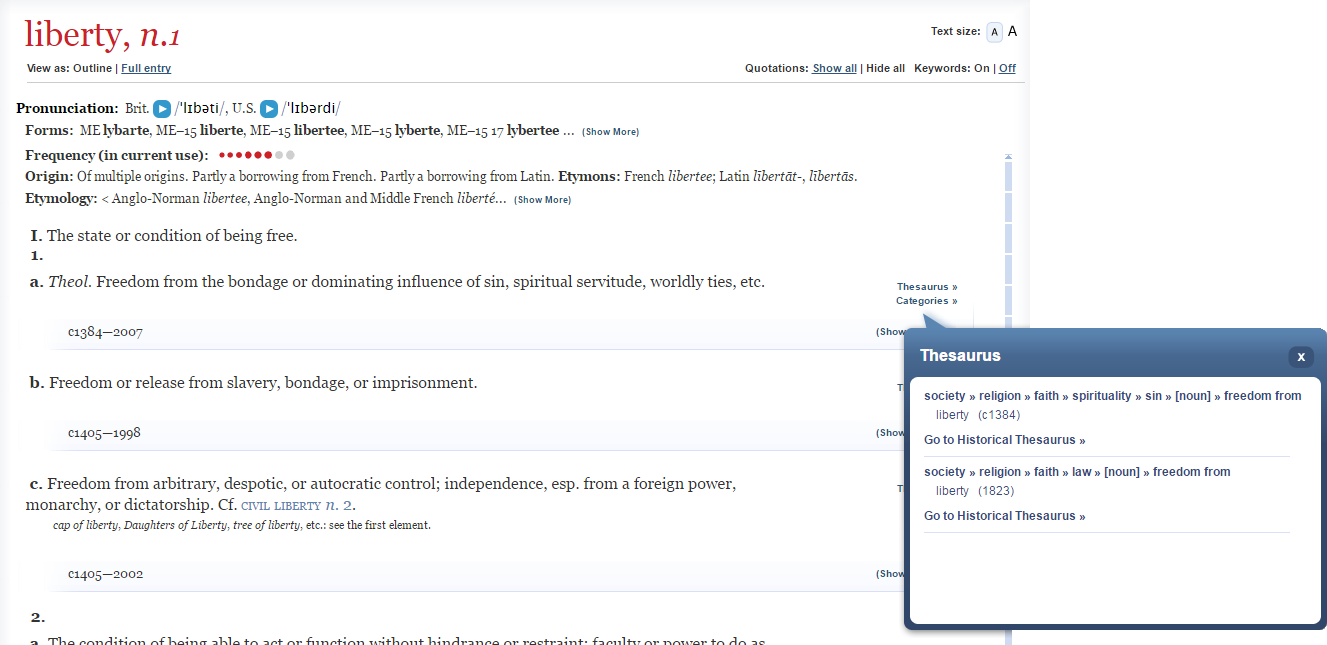
\includegraphics{Stolk_thes-content/fig/OED-sv-liberty-n1}
		}
	}
	\caption[]{\label{fig:Stolk_thes-content:OED-sv-liberty-n1} Entry `liberty, n.1' in \textit{OED Online} (3rd edn). A pop-up window, on the right, indicates that sense 1a is assigned to two categories of the historical language thesaurus \textit{HTE2}.}
\end{figure} 

% insert Figure 5: The category ``civil liberty'' in HTE2. Two senses of the lexeme liberty are included in this category. The first of these links to sense 1c of dictionary entry liberty, n.1; the second to sense 2c.

\begin{figure}[htb]
    \centering
	\framebox[0.8\textwidth]{
		\scalebox{0.7}[0.7]{
			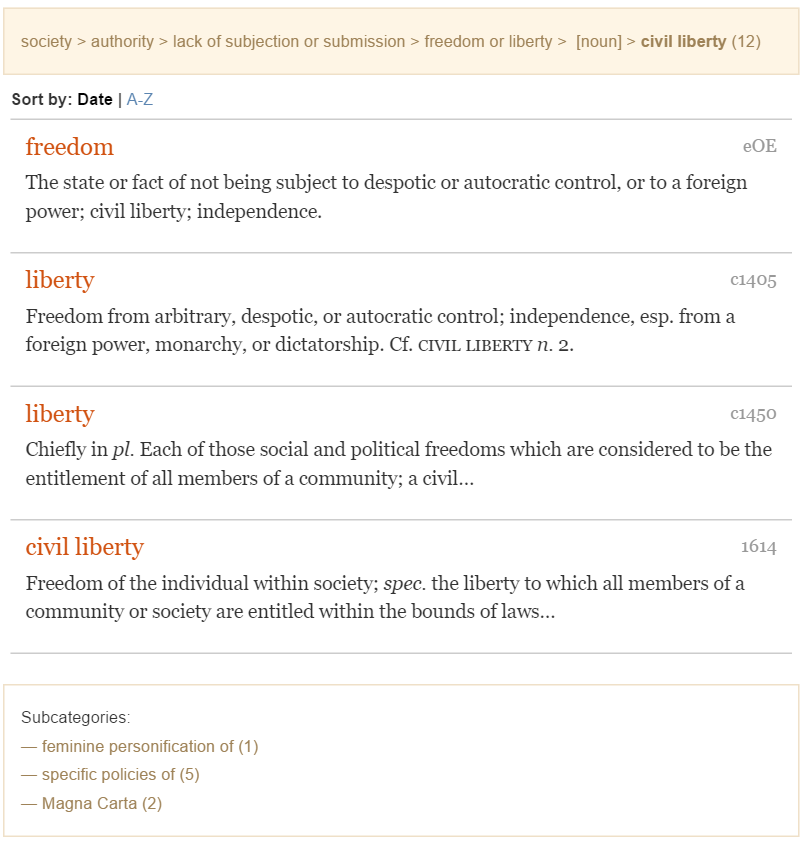
\includegraphics{Stolk_thes-content/fig/HTE2-cat-civilliberty.png}
		}
	}
	\caption[]{\label{fig:Stolk_thes-content:HTE2-cat-civilliberty} The category ``civil liberty'' in \textit{HTE2}. Two senses of \textit{liberty} are included in this category. The first of these links to sense 1c of \textit{OED Online} entry `liberty, n.1'; the second to sense 2c.}
\end{figure} 

\subsection{Structure of lexical senses}
For any lexicographical work, including thesauri, the question of which information is provided per lexical sense depends on the audience and purpose of the work as its editors perceived it.\footnote{%B. T. S. Atkins and M. Rundell,
Atikins and Rundell, \textit{The Oxford Guide to Practical Lexicography}% (Oxford, 2008)
, p. 200.} The structure of senses in ordinary dictionaries, for instance, typically includes the part of speech, definition, and possibly a number of other components, such as quotations and meta language indicating register or regional use.\footnote{%B. T. S. Atkins and M. Rundell,
%Atikins and Rundell, \textit{The Oxford Guide to Practical Lexicography}
% (Oxford, 2008) %IBID
Ibid., pp. 200-57.} These components aid in clarifying the unknown: the meaning and usage of a certain word or phrase. For thesauri, the unknown is not the meaning, which is captured in the topical system, but the words or phrases that express that meaning. Hence thesauri often omit definitions for their senses; information on their meaning is already indicated (to a certain degree) through their placement in the overarching hierarchy.\footnote{\textit{TOE2}, p.xxxiii; \textit{HTE1}, p. xxii.} Moreover, any additional information per lexical sense, such as etymology or register, may already be captured in other reference works and is sometimes considered superfluous in thesauri.\footnote{\textit{ShT}, p. x; \textit{ScT}, p. xv.} 
%Indeed, if a thesaurus presents any additional information for its lexical senses, it is meant to make the thesaurus more useful for the targeted purpose and audience. 
Nevertheless, the historical language thesauri analysed in the chapter all include such additional information (such as part of speech in \textit{ShT} and use restricted to poetic texts in \textit{TOE}), which may be attributed to their purpose of acquainting users with words and phrases from a historical context rather than a contemporary one with which they may be more familiar. What additional information is present, and in which of these thesauri, will be discussed shortly.

The order of components presented for a lexical sense typically adheres to a strict sequence in lexicographic works.\footnote{Atkins and Rundell, \textit{The Oxford Guide to Practical Lexicography}, pp. 200–57.} The order decided upon by editors, which may vary between such works, is mainly intended to present the user of the resource with information in a structured and consistent manner. Through such a sequence, and through visual clues to distinguish the components, users are aided in recognising the information presented and in locating the elements in which they are interested. %Looking up specific information becomes easier when contents are organised according to a sensible system.
Although each historical language thesaurus edition may adhere to its own sequence of components, the works analysed here tend to start with a form of the lexical item (its head-form), followed by the part of speech and, if such components are included, the definition, usage features, and lastly external references. 
%The components included in these thesauri -- i.e., part of speech, definition, language, usage features, and external references -- are discussed in the following subsections.
These components are discussed, separately, in the following subsections.


\subsubsection{Part of speech}
The majority of the historical language thesauri analysed explicitly state the part of speech for their lexical senses. This information is presented either per sense separately (\textit{ShT}, \textit{ScT}, \textit{BTH}) or, more often, per category or set that groups lexical senses (\textit{LSM}, \textit{HTS}, all editions of \textit{HTE}, and the electronic editions of \textit{TOE}). The remaining thesauri leave it to the user to infer the part of speech of lexical senses from the meaning indicated by the names of the categories (\textit{DSSPIEL}, print editions of \textit{TOE}). In these last-mentioned thesauri, the part of speech is explicitly indicated only under special circumstances, such as when the editor considers the part of speech to be unclear from the context. To illustrate, words located under \textit{DSSPIEL} category ``1.85 \textit{Burn}'' are explicitly labelled as verbs in order to ensure they are not interpreted as nouns. It should be noted that the indication of a part of speech for a lexical sense also holds, of course, for the lexeme to which that sense is attributed. 

\subsubsection{Definition}
A definition for lexical senses is another component found amongst the historical language thesauri of Scots and English.
As thesauri already indicate the meaning of lexical senses through their placement in the topical system, definitions are often omitted in the structure of the lexical sense. In fact, the only thesauri analysed that contain such definitions for each of their lexical senses (again, beyond the definitions that can be construed using the topical system) are those covering the Scottish lexis: \textit{ScT} and \textit{HTS}. In her review of \textit{ScT}, Betty Kirkpatrick explains the need for the definitions for these particular thesauri:
\begin{quotation} \noindent
There are innovations in the Scots Thesaurus. Unlike other thesauruses it has definitions. This is not only essential for people from outside Scotland but for many Scots living in Scotland who need to be acquainted or re-acquainted with their native tongue.\footnote{%B. 
Kirkpatrick, Review of \textit{ScT}, %\textit{International Journal of Lexicography} 5.4 (1992), 305–9 (
p. 306.}
\end{quotation}
Here, therefore, the inclusion of definitions is warranted by the intended audience for these thesauri. The need to know what a word exactly means is deemed important enough for its inclusion as opposed to assuming that users are already aware of the distinctions between related or synonymous words, are not interested in such information, or are willing to consult other reference works. For the majority of the historical language thesauri analysed in this chapter, users are indeed encouraged to consult other sources for exact definitions (as well as for other components) when the need for such information arises.\footnote{\textit{ShT} dubs existing dictionaries ``indispensible companions to the present work'' (p. x). \textit{HTE} encourages the user to ``return to the \textit{OED} and gather fresh information'' on lexical senses (\textit{HTE1}, p. xiv). \textit{TOE} informs its users of the general need for dictionaries next to thesauri: ``Compared with a dictionary, any thesaurus is somewhat of a blunt instrument, sacrificing semantic or grammatical specificity to breadth of conceptual coverage.'' (\textit{TOE2}, p. xxxv). 
%It is therefore unsurprising that \textit{TOE3}, the electronic edition of \textit{TOE}, provides the means to search for its categorized items in digital Old English dictionaries available online.
}

\subsubsection{Language}
The language of a lexical sense is indicated explicitly in only two of the historical language thesauri analysed. The component is found in \textit{DSSPIEL} and \textit{BTH}, multilingual thesauri fashioned specifically for the purpose of contrasting words from multiple languages that denote the same concept (Indo-European languages, in the case of \textit{DSSPIEL}; Anglo-Norman and Middle English in \textit{BTH}). \textit{ShT}, too, may be considered a multilingual thesaurus, as its editor has opted not to confine the thesaurus to Shakespeare's attested English lexis only. The ``foreign words'' found in Shakespeare's works, far fewer in number than the English ones, ``are normally those in foreign-language contexts only''.\footnote{\textit{ShT}, p. xiii.} That is to say, characters in a play may be French or Italian and converse in their native tongues. The play \textit{Henry V}, for instance, contains a scene in which the French princess Catherine tries to learn a number of English words from her maid.\footnote{Shakespeare, \textit{Henry V}, %ed. J. D. Mardock, Broadview Internet Shakespeare Editions (Peterborough, Ontario 2014), 3.4. 
pp. 140–2.} The conversation is performed entirely in French, apart from those words that are being taught, of course. To indicate this distinction in language in Shakespearian vocabulary, \textit{ShT} marks foreign words with a label (`lat.' for Latin, `fr.' for French, and `it.' for Italian). The other thesauri analysed deal with the lexis from what is considered a single language, albeit with varying dialects or variants. An explicit reminder of the language at every lexical sense contained within is, understandably, deemed unwarranted by their editors.

\subsubsection{Usage features}

Information on usage and distribution is, according to the editor of \textit{LSM}, ``not normally included'' in the structure of lexical senses in thesauri.\footnote{\textit{LSM}, p. 5.} In contrast, historical language thesauri appear to be an exception to this rule: five out of the eight analysed include information on usage features. One must conclude, therefore, that users of historical language thesauri are thought to require, or rather desire, more information on the included lexical senses than users of most contemporary thesauri do. Of course, historical lexis may take on forms that are significantly different from contemporary ones or may have undergone significant changes in their meaning or use --- changes that are worth pointing out to users of historical language thesauri through, amongst others, indications of usage features.

\hyperref[Appendix1.B]{Appendix 1.B} provides an overview of which kinds of usage information are conveyed systematically in the historical language thesauri analysed. These include indications of restricted use of a given word or phrase to a specific genre, region, dialect, or medium. Most of these features are indicated through labels (e.g., `poetic' for words specific to poetic diction). In contrast, diachronic usage features are captured in \textit{LSM} and \textit{HTE} through dates of currency instead. Here, a label is used solely for the historical period of Old English (abbreviated to `OE'), since exact dating of texts and language use for this early medieval period is not as straightforward as for later periods of English. %Presentations of usage features may, unfortunately, obfuscate whether these features are specific to a lexical sense, apply to the lexeme in its entirety, or are attributed to both.

\subsubsection{External reference}
\label{sect:Stolk_thes-content:ExternalReference}

The final component found in historical language thesauri of Scots and English is an external reference. In fact, the majority of the historical language thesauri advise the user to pick up additional reference works for further or more detailed information on their included lexis. Many of these thesauri have taken dictionaries as the source of their information, which entails that references to the source material can be maintained during the editorial process. In cases where not all information from a source dictionary is transferred to the resulting thesaurus, references to the source material can offer users valuable insights beyond information the thesaurus editors deem to warrant including directly. To illustrate, \textit{HTE} abandons indications of etymology found in the \textit{OED}.

The form in which external references are made differs between print and electronic editions of the thesauri analysed. Print editions typically refer the user to a source dictionary in the introduction. Providing an external reference per lexical sense instead would offer little to no additional benefit, as it requires the reader to manually access the contents of the external reference work and locate the sense in question. Digital editions of thesauri, in contrast, are capable of facilitating the user in this process. In these editions, references can be offered by hyperlinks that lead the user to specific locations in other digital bodies. Such efficient links are available in the electronic editions of \textit{TOE}, \textit{HTE}, and \textit{HTS}. Hyperlinks per lexical sense refer the user in these cases to either the exact corresponding item in the source dictionary (with \textit{HTS} and \textit{HTE2}) or to a search for the item using the search engine of an external digital body (with \textit{TOE4} and \textit{HTE3}). Of course, external references need not only lead to dictionaries. 

%Lexical senses captured in historical language thesauri can be viewed in contexts other than source dictionaries, too. 
\textit{TOE4} offers the user external references to University of Toronto's \textit{Dictionary of Old English Web Corpus}. These references allow the user to automatically search for attestations of a word or phrase from \textit{TOE} (with that particular spelling) amongst Old English texts that have come down to us, effectively offering insights into the contexts in which the item is known to have been used. %Other external references, such as to specialized fields of research on the lexical senses, would also be possible in a digital setting and certainly an advantage for those users who are looking to learn more about a lexical sense, or a set thereof, in existing linguistic or literary contexts.
Having discussed this final component and thereby the structure of lexical senses in their entirety, I turn to other aspects of these items found in historical language thesauri: their order when co-ordinated and, afterwards, their identification.


\subsection{Order of co-ordinate lexical senses}

Co-ordinate lexical senses in historical language thesauri, i.e., senses located at the same thesaurus category, 
are displayed in a systematic order. This order, as Kay and Alexander observe, appears to depend on the availability of diachronic usage information:
\begin{quotation} \noindent
  Within the macrostructure, historical language thesauruses which regard their data as belonging to a single period will usually display synonyms in alphabetically organized lists. Those with a diachronic spread will order lists chronologically, or will compromise by including some information about dates of use within an alphabetical list, as \textit{The Scots Thesaurus} (1990) does.\footnote{Kay and Alexander, `Diachronic and Synchronic Thesauruses', p. 372.} 
\end{quotation}
Indeed, the historical language thesauri that include diachronic usage information in a detailed manner (i.e., \textit{LSM} and \textit{HTE}) order their senses chronologically.\footnote{\textit{LSM}, p. 15; \textit{HTE1}, p. ix.} \textit{ScT}, as noted, employs an alphabetical ordering instead. Diachronic usage information in \textit{ScT} is rather limited, effectively dividing senses into those that are considered obsolete and those that are not. An ordering based on this rather coarse distinction would still require co-ordinate lexical senses to be organized within these two groups. In lieu of a better alternative, the otherwise meaningless alphabetic ordering can always be employed to order senses. In fact, it should be noted that both \textit{LSM} and \textit{HTE} indeed fall back on alphabetical ordering for co-ordinate senses that have identical diachronic usage information.\footnote{\textit{LSM}, p. 28; \textit{HTE1}, p. xxiii.}

Although most historical language thesauri without diachronic usage information employ an alphabetical ordering of co-ordinate lexical senses, not all of them can be said to do so. An alphabetical ordering is applied in \textit{ScT}, \textit{ShT}, \textit{TOE}, and \textit{HTS}.\footnote{It should be noted that the alphabetical ordering might be on a particular form of the categorized items. In \textit{TOE3}, for instance, the category ``01|01 (n) Earth, world :: As God's creation'' contains \textit{gesceaft}, which is found after \textit{sǣ} and \textit{eorþe}. The reason for this ordering is that some Old English words are found in texts both with and without the \textit{ge}- prefix, and that therefore some lexicographical bodies ignore this prefix in their alphabetical ordering (see, for instance, \textit{DOE}).} These are thesauri that capture the lexis of a single language or, in the case of \textit{ShT}, at least for the majority of its items. In contrast, the multilingual thesaurus \textit{DSSPIEL} presents the items in three columns based on their language.\footnote{\textit{DSSPIEL} does not make this order or the reason behind it explicit, suggesting the order is considered logical enough to the readers interested in the comparative linguistics with which the book is concerned.} The first column displays the synonyms for a particular concept taken from Hellenic languages, then those from Italic languages, followed by Celtic ones. The second column displays the lexical senses taken from Germanic languages. The third and last column those of Balto-Slavic and afterwards Indo-Iranian languages. Within these groups, too, the order of the languages is set. For the Germanic ones, for instance, Gothic is followed by Old Norse, Danish, Swedish, Old English, Middle English, New English, Dutch, Old High German, Middle High German, and lastly, New German.\footnote{These are the names for the languages as adopted by \textit{DSSPIEL} (see pp. 1–2).} Here it is possible to see that the order is again based on more than simply chance or the alphabet, as younger variants of a language are preceded by older ones (e.g., New English is preceded by Old and Middle English). In short, the order of lexical senses in a historical language thesaurus can depend on any piece of information associated with them --- not limited to diachronic information. This finding suggests that other information, too, such as diatopic usage information, could be used to order lexical senses in historical language thesauri yet to be developed.

As the above discussion has shown, the order of co-ordinate lexical senses is based on explicit information captured for each sense. Any ordering found in the historical language thesauri analysed does not present new information on the lexical senses or provides a better understanding of how these co-ordinate items relate to one another. Instead, the applied order ensures that users can expect to find an item in a position governed by a system that is -- or rather, should be -- easily grasped.

\subsection{Identification of lexical senses}

Dictionaries and thesauri, both lexicographic works, tend to employ a different identification mechanism for their lexical senses.
%The identification of lexical senses in a thesaurus may differ from that in a typical dictionary, 
The dictionary \textit{OED Online}, for instance, contains the following senses for the adjective \textit{politely}.
\begin{quotation} \noindent
\textbf{politely, \textit{adv}. †1.} Smoothly. Obs. 1598--1730  \textbf{2.} In a polished or refined manner; elegantly. Now rare. 1624--1868  \textbf{3}. Courteously; with good manners; with consideration for the feelings of others. 1748--1993 \footnote{\textit{OED Online}, 3rd edn, s.v. `politely, adv.'. %Accessed on October 18, 2016.
}
\end{quotation}
A reference to one of these three senses typically includes both the headword and the code that identifies the sense within this particular grouping, for example: \textit{OED Online}, 3rd edn, s.v. `politely, adv.', sense 3. In the case of thesauri, this practice can only be applied effectively if they maintain a relation between lexical senses and their lexemes. Only \textit{HTE2}, out of the eight historical language thesauri, does so. Consequentially, lexical senses in thesauri often have to be identified in a manner different from that found in typical dictionaries and utilize the topical system in which senses are positioned.

Lexical senses in a thesaurus are spread across its topical system. Senses that in a dictionary would have been grouped under the same headword may well be found at different locations in a thesaurus. The head-form that identifies such a sense, acting for it as a ``linguistic dummy'', is therefore useful for clear identification only in the context of the category in which that sense is found. References that would include only the head-form of a lexical sense tend to be ambiguous as a result. Referring to ``light'', for instance, is not sufficient to determine whether its sense categorized as ``lamp'' is meant or that as ``relatively small in weight''. The position of a lexical sense in the topical system is therefore, in the majority of historical language thesauri, highly relevant for proper identification. To illustrate, the sense of \textit{franchise} as shown in Figure \ref{fig:Stolk_thes-content:Content-parts} could be identified by referring to ``\textit{franchise} as found in 03.04.10.03 n. Freedom/liberty''.
(The identification and referencing to categories in the topical system has been treated earlier, in section \ref{sect:Stolk_thes-content:categories-id}). 

In some of the historical language thesauri, the head-form along with the location in the topical system is insufficient to refer to a single sense unambiguously. The \textit{ScT} category ``15.6.13 Anger'', for instance, contains the following entry:
\begin{quotation} \noindent
	\textbf{scunner} \textbf{1} a nuisance. \textbf{2} a troublesome person.
\end{quotation}
Here, the grouping of senses is similar to that found in typical dictionaries. Hence there is the need for including the number that identifies a specific sense within the grouping, too, in references to a lexical sense. The location in the topical system remains relevant even in cases like \textit{ScT}, which appear at first glance to resemble a dictionary in terms of its identification and grouping system. The groupings of senses based on head-form and number are guaranteed to be unique only per category. Thus, one finds the head-form ``able'' in \textit{ShT} without any further sense division in both category ``9.1.1 General'', in the sense of being physically fit, and in ``10.4 Eating and drinking'', in the sense of having an appetite. Only their definition and locations in the topical system can be used to distinguish the two senses. In short, the identification of lexical senses in a thesaurus typically consists of a head-form and perhaps further identification within a group. However, these identifications are not necessarily unique throughout the thesaurus and references should therefore include the position of such senses in the overarching topical system. 
%With the structure, co-ordination, and identification of lexical senses covered, I now move on to the third main component found in many thesauri: synonymy.

\section{Synonymy}
\label{sect:Stolk_thes-content:Synonymy}

The overarching topical system of a thesaurus provides a structure for words and phrases in their various senses. %Users are thus able to move from the known to the unknown: from meaning to words or phrases that express this meaning.\footnote{Hüllen, \textit{A History of Roget's Thesaurus}, pp. 282–3.} 
Senses grouped by thesaurus categories are, per definition, sets with a similar or related meaning. With most historical language thesauri this chapter covers -- but not all -- such sets indicate an even stronger semantic tie: one of synonymy. The words \textit{start}, \textit{begin}, and \textit{commence}, for instance, can be considered synonymous, since they denote the same concept. In which cases words or phrases are deemed synonymous depends on the definition of the relation to which is adhered.

The semantic relation of synonymy has four prominent definitions in linguistics. Arranged from most to least restrictive, these various types of synonymy are called absolute, perfect, cognitive, and near-synonymy (see Table \ref{table:Stolk_thes-content:synonymy-def}). The most restrictive of these, absolute synonymy, requires lexemes to have the same meaning and use for all their senses. Whether this strictest variant of synonymy truly exists is debatable. Words or phrases may not only differ in the meanings they carry but also in some other aspects, such as their connotation, register, or frequency in use.\footnote{Murphy, \textit{Encyclopedia of Language and Linguistics}, %2nd edn, ed. K. Brown (Oxford, 2006), 
s.v. `Synonymy'.} The other three definitions consider synonymy to be a relation between lexical senses instead of lexemes in all their senses. Perfect synonymy of two lexical senses requires them to be the same in meaning and use regardless of the context in which they are used. Cognitive synonymy stipulates that senses need to be the same in meaning apart from any possible variation in usage between them. The least restrictive definition, that of near-synonymy, calls for a similarity of meaning and requires two senses to be substitutable only in specific contexts. 

\begin{table}[h!]
    \centering
    \small
    { \RaggedRight
    \begin{tabular}{lll}
    \toprule
        \textbf{Relation} & \textbf{Between} & \textbf{Example} \\
    \midrule
Absolute synonymy  & lexemes  & \textit{anyone}=\textit{anybody} \\
Perfect synonymy   & lexical senses & \textit{crucifer}=\textit{brassica} (`cabbage') \\
Cognitive synonymy & lexical senses & \textit{peritonsillar abscess}=\textit{quinsy} (`illness') \\
Near-synonymy      & lexical senses & \textit{to pacify}=\textit{to placate} (`to calm') \\
    \midrule
    \end{tabular}
    }
    \caption[]{\label{table:Stolk_thes-content:synonymy-def}Examples of different definitions of synonymy.\protect\footnotemark}
\end{table}
\footnotetext{Based on Murphy, `Meaning Relations in Dictionaries%: Hyponymy, Meronymy, Synonymy, Antonymy, and Contrast
    ', %in \textit{The Oxford Handbook of Lexicography}, ed. P. Durkin (Oxford, 2016), pp. 439–56 (
    pp. 447–8.}

Not every thesaurus indicates relations of synonymy according to even the most forgiving of definitions. \textit{ShT} and \textit{ScT}, for instance, omit such indications. To illustrate, \textit{ScT} contains the category ``6.2.3 Shipping, navigation'' in which the noun \textit{spulyie} and the verb \textit{stell} are adjacent entries. The sense of the former is indicated as ``jetsam, anything cast ashore''; the latter as ``load (a ship) evenly, trim the cargo in (a ship)''. These two senses can hardly be considered interchangeable; even the parts of speech of the items differ.\footnote{Synonymous lexical items are typically thought, in order to be interchangeable, to require a shared part of speech (Murphy, `Meaning Relations in Dictionaries', p. 439). Be that as it may, some scholars ``claim that synonymy is possible between words belonging to different parts of speech (as between the verb \textit{sleeping} and adjective \textit{asleep})'' (Stanojević, `Cognitive Synonymy: A General Overview', %\textit{Linguistics and Literature} 7.2 (2009), 193–200 [
p. 194.} Adjacency here, therefore, does not indicate synonymy. Similarly, \textit{ShT} positions the verb \textit{overblow} and the noun \textit{sea-storm} alongside each other in category ``01.06 Wind, storm''. These, too, can not be considered synonymous according to any of the four established definitions. In short, grouped items presented at the same location in the topical system of these two thesauri do not indicate anything beyond belonging to the same semantic field.

Although not found in \textit{ShT} and \textit{ScT}, sets of synonyms are present in all the other historical language thesauri analysed: \textit{DSSPIEL}, \textit{TOE}, \textit{LSM}, \textit{HTE}, \textit{HTS}, and \textit{BTH}. The degree to which members of such a set are considered synonyms may vary across these thesauri. \textit{TOE}, for instance, asserts that its grouped items, although they share ``at least one component of meaning'', are to be seen as loosely synonymous only.\footnote{\textit{TOE2}, p. xxxiii.}
\begin{quotation} \noindent
No claim is made that the words assigned to each group are synonyms in any strict sense of the term, i.e. that they are mutually substitutable in all or most contexts. Rather, they are loosely synonymous terms which express the concept defined by the headings, which will itself often be a descriptive phrase rather than a single word.\footnote{\textit{TOE2}%Ibid.
, p. xxxiii.}
\end{quotation}
The introduction in \textit{LSM} contains a similar statement:
\begin{quotation} \noindent
Grouping terms together in a thesaurus, even in a thesaurus as detailed as this, does not imply absolute synonymy. Many scholars doubt whether absolute interchangeability is actually possible [...].\footnote{\textit{LSM}, p.15. Coleman refers to publications by Ullman, Firth, Harris, and Baldinger in which doubts about absolute synonymy are raised.}
\end{quotation}
In light of these statements, it must come as no surprise that the least restrictive form of synonymy, near-synonymy, has been called ``the staple of thesauruses''.\footnote{Murphy, `Meaning Relations in Dictionaries', p. 448.} Lexical senses grouped as synonyms -- or rather, as near-synonyms -- therefore possess a certain degree of interchangeability. 

%\subsection{Structure of sets of synonyms}
%The structure of any group of lexical senses boils down to a matter of membership. That is to say, a group in a thesaurus contains any number of senses that, to a certain extent, overlap. Such groupings are already in place through categories in the overarching topical systems of thesauri. Synonymy between senses, however, indicates a stronger semantic tie than may be the case with categorisation. For those thesauri that contain sets of synonyms -- i.e., \textit{DSSPIEL}, \textit{TOE}, \textit{LSM}, \textit{HTE} \textit{HTS}, and \textit{BTH} -- it is therefore important to understand to what extent, if any, they differentiate in their presentation between sets of synonyms and categories containing lexical senses.


The presence of synonymy is, in editions of the historical language thesauri analysed, not presented differently from the absence of synonymy (or, to be more precise, from omissions of their presence). To illustrate, all senses in \textit{HTE1} positioned in the same category are considered synonyms; those in \textit{ShT} are not claimed to be (and often are not).\footnote{\textit{HTE1}, p. xxv.} 
In thesauri that capture synonymy, therefore, categories can act as sets of synonyms as well as semantic fields. Even so, there are notable differences between the two of which users should be aware.

The first and perhaps most obvious difference between synonym sets and categories representing a semantic field is that the former imply that the relation between its grouped members is one of interchangeability in certain contexts, whereas this is not necessarily the case for members belonging to a category within any given thesaurus. (As mentioned, this lack of interchangeability for grouped items is found in \textit{ShT} and \textit{ScT}.) 

The second difference between synonym sets and categories concerns the membership of lexical senses. Lexical senses located at a particular category are members of that category and any superordinate categories, which can be viewed as generalizations of the semantic field.\footnote{\textit{HTE1}%Ibid.
, p. xviii.} If these same senses are known to be synonymous, that is, part of a synonym set, they are \textit{not} also synonymous with the senses found in those superordinate categories. In Figure \ref{fig:Stolk_thes-content:synset-vs-semfield}, for example, the lexical sense of \textit{freedom} at category ``Freedom/liberty'' is not synonymous  with \textit{command} and the other senses listed at ``Authority''. This sense of \textit{freedom} is, however, categorized as belonging to categories ``Society'', ``Authority'', ``Lack of subjection'', and ``Freedom/liberty''. 
Simply put, the placement of a lexical sense in a thesaurus may posit it as part of a specific synonym set and typically signifies the sense belongs to multiple categories --- one that is the most specific and others that are superordinate. These differences, as shown for \textit{HTE} in the previous paragraph, tend to be left implicit in the presentation of the thesauri, and may be left implicit in the way the lexemes and their senses are stored in the datasets behind electronic editions, too.\footnote{A case in point is \textit{TOE4}, of which the database leaves relations of synonymy implicit (see Chapter 6).}
%Having discussed synonymy, the last of the three main components of thesauri, I continue to examine two information elements present with both the topical system and lexical senses.   
%\footnote{As Chapter 6 of this dissertation shows, \textit{TOE} does not capture lexemes that group senses. The Linguistic Linked Data version of this thesaurus, TOE-LLD, added these items (see Chapter 7).}

\begin{figure}[htbp]
	\framebox[\textwidth]{
		\scalebox{0.65}[0.65]{
		    % Graphic for TeX using PGF
% Title: C:\Users\Sander\Documents\Dropbox\PhD\images\Content-LexicalSense-Membership.dia
% Creator: Dia v0.97.2
% CreationDate: Wed Apr 13 17:53:15 2022
% For: Sander
% \usepackage{tikz}
% The following commands are not supported in PSTricks at present
% We define them conditionally, so when they are implemented,
% this pgf file will use them.
\ifx\du\undefined
  \newlength{\du}
\fi
\setlength{\du}{15\unitlength}
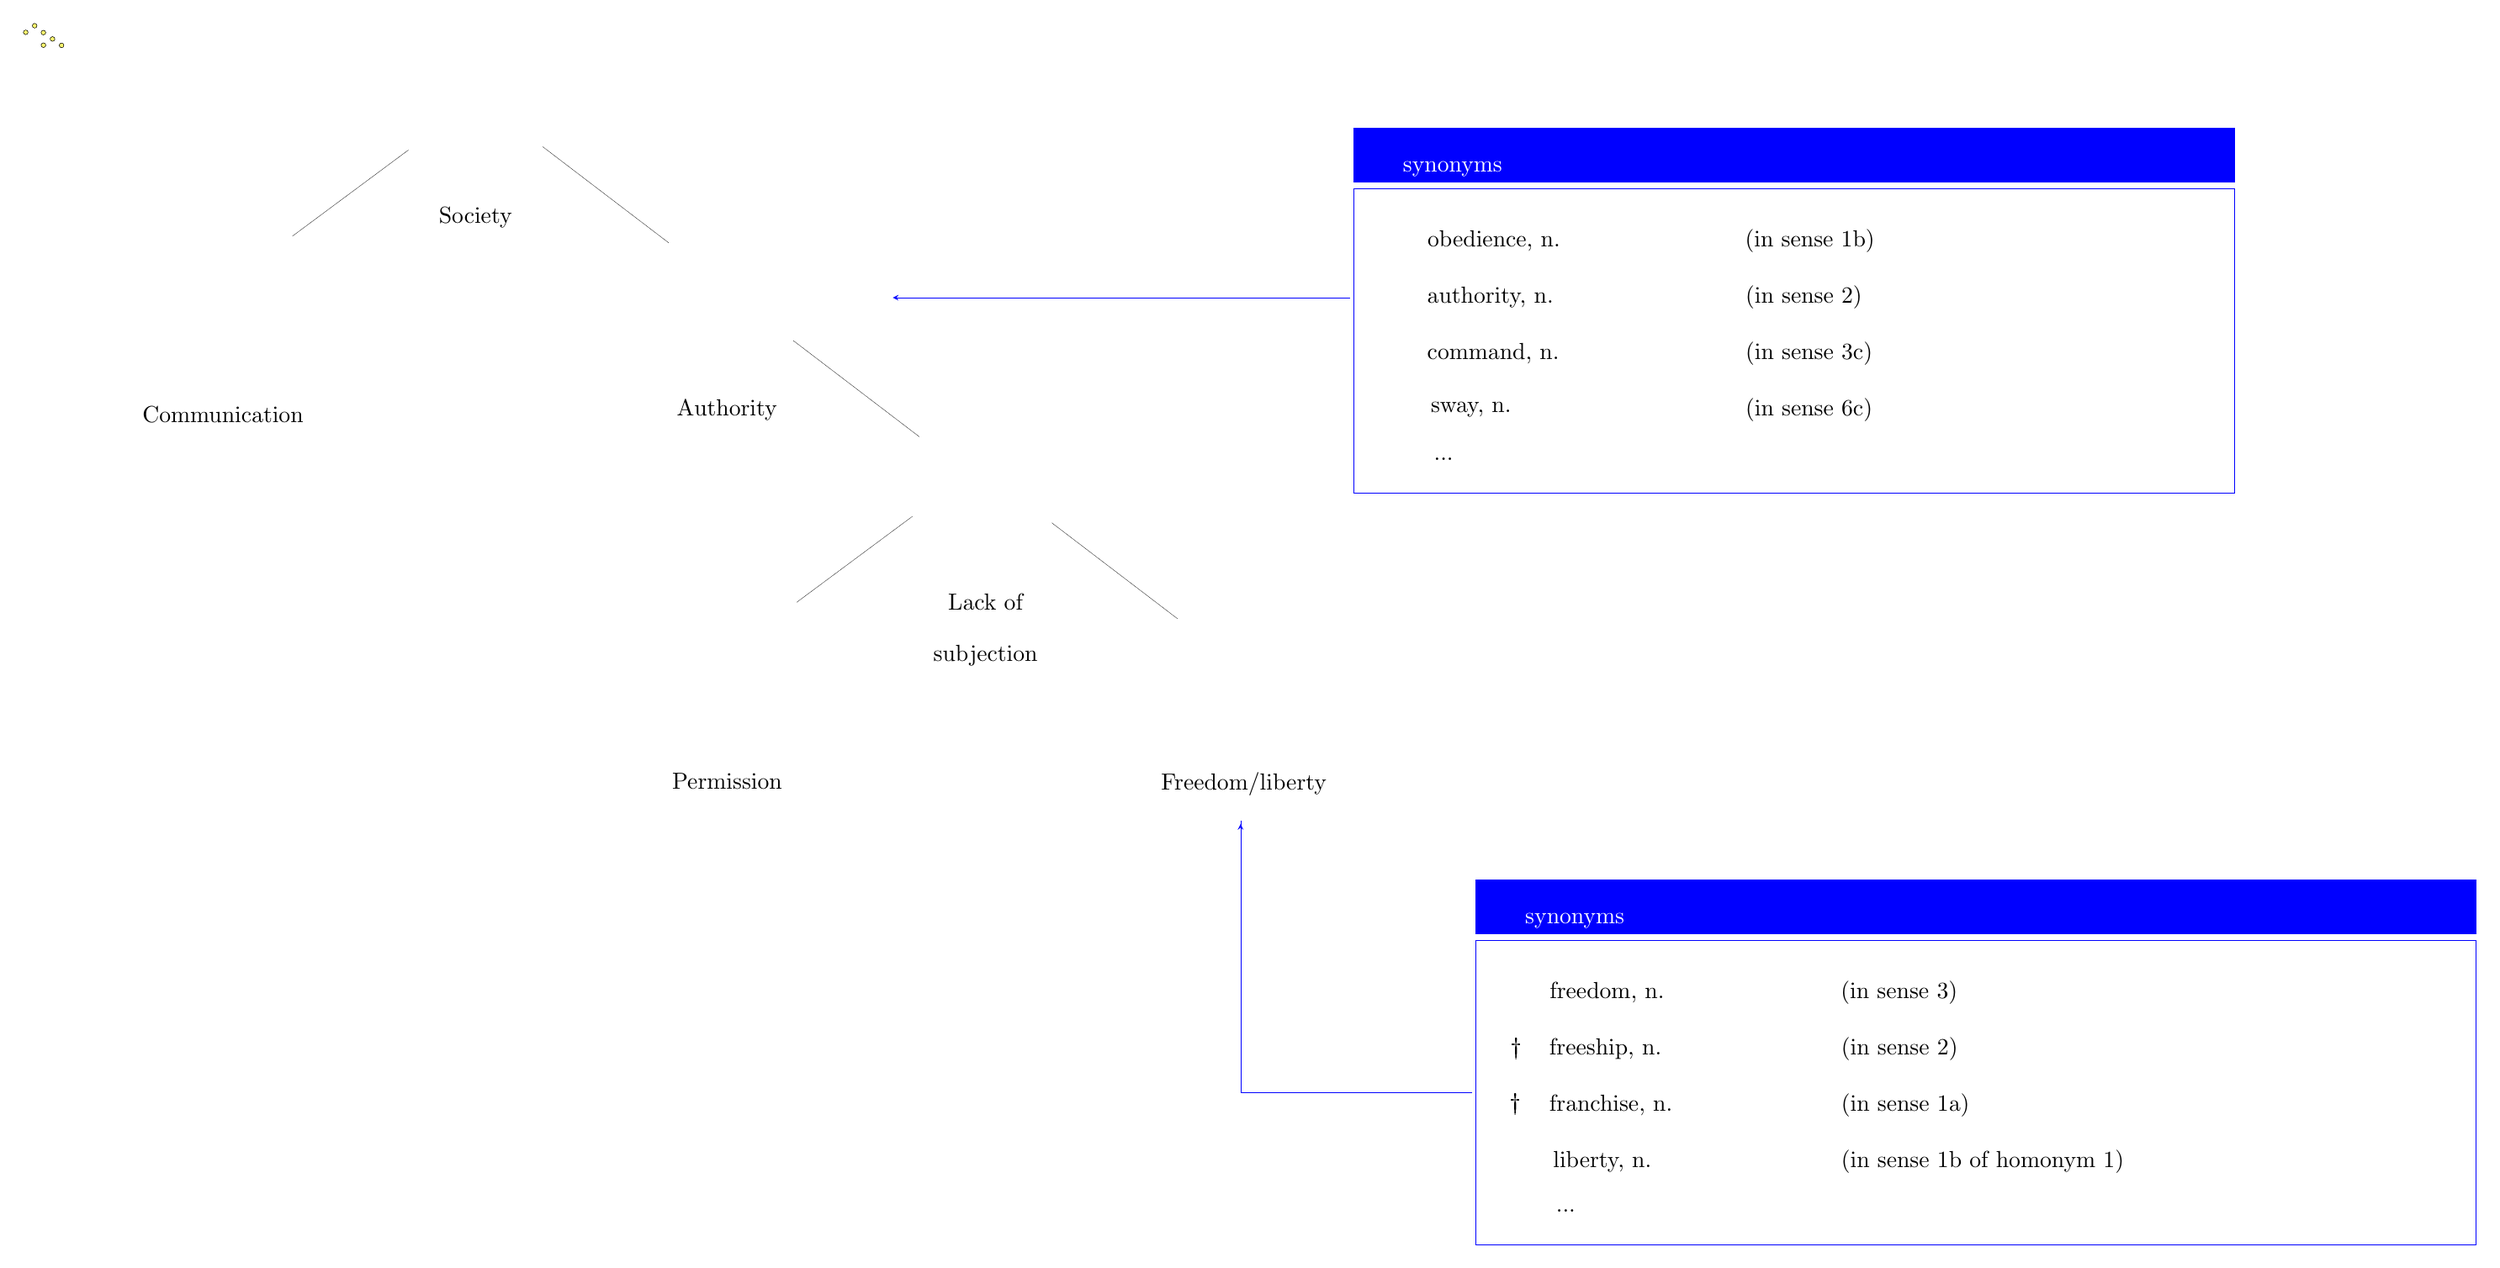
\begin{tikzpicture}
\pgftransformxscale{1.000000}
\pgftransformyscale{-1.000000}
\definecolor{dialinecolor}{rgb}{0.000000, 0.000000, 0.000000}
\pgfsetstrokecolor{dialinecolor}
\definecolor{dialinecolor}{rgb}{1.000000, 1.000000, 1.000000}
\pgfsetfillcolor{dialinecolor}
\pgfsetlinewidth{0.100000\du}
\pgfsetdash{}{0pt}
\pgfsetdash{}{0pt}
\pgfsetbuttcap
\pgfsetmiterjoin
\pgfsetlinewidth{0.100000\du}
\pgfsetbuttcap
\pgfsetmiterjoin
\pgfsetdash{}{0pt}
\definecolor{dialinecolor}{rgb}{1.000000, 0.984314, 0.435294}
\pgfsetfillcolor{dialinecolor}
\pgfpathellipse{\pgfpoint{14.600000\du}{6.900000\du}}{\pgfpoint{1.000000\du}{0\du}}{\pgfpoint{0\du}{1.000000\du}}
\pgfusepath{fill}
\definecolor{dialinecolor}{rgb}{0.000000, 0.000000, 0.000000}
\pgfsetstrokecolor{dialinecolor}
\pgfpathellipse{\pgfpoint{14.600000\du}{6.900000\du}}{\pgfpoint{1.000000\du}{0\du}}{\pgfpoint{0\du}{1.000000\du}}
\pgfusepath{stroke}
\pgfsetbuttcap
\pgfsetmiterjoin
\pgfsetdash{}{0pt}
\definecolor{dialinecolor}{rgb}{0.000000, 0.000000, 0.000000}
\pgfsetstrokecolor{dialinecolor}
\pgfpathellipse{\pgfpoint{14.600000\du}{6.900000\du}}{\pgfpoint{1.000000\du}{0\du}}{\pgfpoint{0\du}{1.000000\du}}
\pgfusepath{stroke}
\pgfsetlinewidth{0.100000\du}
\pgfsetdash{}{0pt}
\pgfsetdash{}{0pt}
\pgfsetmiterjoin
\definecolor{dialinecolor}{rgb}{1.000000, 1.000000, 1.000000}
\pgfsetfillcolor{dialinecolor}
\fill (22.000000\du,13.850000\du)--(22.000000\du,18.450000\du)--(37.100000\du,18.450000\du)--(37.100000\du,13.850000\du)--cycle;
\definecolor{dialinecolor}{rgb}{0.000000, 0.000000, 1.000000}
\pgfsetstrokecolor{dialinecolor}
\draw (22.000000\du,13.850000\du)--(22.000000\du,18.450000\du)--(37.100000\du,18.450000\du)--(37.100000\du,13.850000\du)--cycle;
% setfont left to latex
\definecolor{dialinecolor}{rgb}{0.000000, 0.000000, 0.000000}
\pgfsetstrokecolor{dialinecolor}
\node[anchor=west] at (23.050000\du,17.200000\du){liberty, n.};
% setfont left to latex
\definecolor{dialinecolor}{rgb}{0.000000, 0.000000, 0.000000}
\pgfsetstrokecolor{dialinecolor}
\node[anchor=west] at (23.000000\du,14.650000\du){freedom, n.};
\pgfsetlinewidth{0.100000\du}
\pgfsetdash{}{0pt}
\pgfsetdash{}{0pt}
\pgfsetmiterjoin
\pgfsetbuttcap
{
\definecolor{dialinecolor}{rgb}{0.000000, 0.000000, 1.000000}
\pgfsetfillcolor{dialinecolor}
% was here!!!
\pgfsetarrowsend{stealth}
{\pgfsetcornersarced{\pgfpoint{0.000000\du}{0.000000\du}}\definecolor{dialinecolor}{rgb}{0.000000, 0.000000, 1.000000}
\pgfsetstrokecolor{dialinecolor}
\draw (21.949713\du,16.150000\du)--(18.450000\du,16.150000\du)--(18.450000\du,12.100000\du)--(18.450000\du,12.100000\du);
}}
\definecolor{dialinecolor}{rgb}{1.000000, 1.000000, 1.000000}
\pgfsetfillcolor{dialinecolor}
\fill (16.050000\du,13.805000\du)--(16.050000\du,14.550000\du)--(16.050000\du,14.550000\du)--(16.050000\du,13.805000\du)--cycle;
% setfont left to latex
\definecolor{dialinecolor}{rgb}{0.000000, 0.000000, 0.000000}
\pgfsetstrokecolor{dialinecolor}
\node at (16.050000\du,14.400000\du){};
\definecolor{dialinecolor}{rgb}{1.000000, 1.000000, 1.000000}
\pgfsetfillcolor{dialinecolor}
\fill (12.726250\du,8.155000\du)--(12.726250\du,9.700000\du)--(16.473750\du,9.700000\du)--(16.473750\du,8.155000\du)--cycle;
% setfont left to latex
\definecolor{dialinecolor}{rgb}{0.000000, 0.000000, 0.000000}
\pgfsetstrokecolor{dialinecolor}
\node at (14.600000\du,8.750000\du){Lack of };
% setfont left to latex
\definecolor{dialinecolor}{rgb}{0.000000, 0.000000, 0.000000}
\pgfsetstrokecolor{dialinecolor}
\node at (14.600000\du,9.550000\du){subjection};
\pgfsetlinewidth{0.100000\du}
\pgfsetdash{}{0pt}
\pgfsetdash{}{0pt}
\pgfsetbuttcap
\pgfsetmiterjoin
\pgfsetlinewidth{0.100000\du}
\pgfsetbuttcap
\pgfsetmiterjoin
\pgfsetdash{}{0pt}
\definecolor{dialinecolor}{rgb}{1.000000, 0.984314, 0.435294}
\pgfsetfillcolor{dialinecolor}
\pgfpathellipse{\pgfpoint{10.695000\du}{4.150000\du}}{\pgfpoint{1.000000\du}{0\du}}{\pgfpoint{0\du}{1.000000\du}}
\pgfusepath{fill}
\definecolor{dialinecolor}{rgb}{0.000000, 0.000000, 0.000000}
\pgfsetstrokecolor{dialinecolor}
\pgfpathellipse{\pgfpoint{10.695000\du}{4.150000\du}}{\pgfpoint{1.000000\du}{0\du}}{\pgfpoint{0\du}{1.000000\du}}
\pgfusepath{stroke}
\pgfsetbuttcap
\pgfsetmiterjoin
\pgfsetdash{}{0pt}
\definecolor{dialinecolor}{rgb}{0.000000, 0.000000, 0.000000}
\pgfsetstrokecolor{dialinecolor}
\pgfpathellipse{\pgfpoint{10.695000\du}{4.150000\du}}{\pgfpoint{1.000000\du}{0\du}}{\pgfpoint{0\du}{1.000000\du}}
\pgfusepath{stroke}
\pgfsetlinewidth{0.100000\du}
\pgfsetdash{}{0pt}
\pgfsetdash{}{0pt}
\pgfsetbuttcap
\pgfsetmiterjoin
\pgfsetlinewidth{0.100000\du}
\pgfsetbuttcap
\pgfsetmiterjoin
\pgfsetdash{}{0pt}
\definecolor{dialinecolor}{rgb}{1.000000, 0.984314, 0.435294}
\pgfsetfillcolor{dialinecolor}
\pgfpathellipse{\pgfpoint{6.940000\du}{1.200000\du}}{\pgfpoint{1.000000\du}{0\du}}{\pgfpoint{0\du}{1.000000\du}}
\pgfusepath{fill}
\definecolor{dialinecolor}{rgb}{0.000000, 0.000000, 0.000000}
\pgfsetstrokecolor{dialinecolor}
\pgfpathellipse{\pgfpoint{6.940000\du}{1.200000\du}}{\pgfpoint{1.000000\du}{0\du}}{\pgfpoint{0\du}{1.000000\du}}
\pgfusepath{stroke}
\pgfsetbuttcap
\pgfsetmiterjoin
\pgfsetdash{}{0pt}
\definecolor{dialinecolor}{rgb}{0.000000, 0.000000, 0.000000}
\pgfsetstrokecolor{dialinecolor}
\pgfpathellipse{\pgfpoint{6.940000\du}{1.200000\du}}{\pgfpoint{1.000000\du}{0\du}}{\pgfpoint{0\du}{1.000000\du}}
\pgfusepath{stroke}
\definecolor{dialinecolor}{rgb}{1.000000, 1.000000, 1.000000}
\pgfsetfillcolor{dialinecolor}
\fill (8.991250\du,5.250000\du)--(8.991250\du,5.995000\du)--(12.398750\du,5.995000\du)--(12.398750\du,5.250000\du)--cycle;
% setfont left to latex
\definecolor{dialinecolor}{rgb}{0.000000, 0.000000, 0.000000}
\pgfsetstrokecolor{dialinecolor}
\node at (10.695000\du,5.845000\du){Authority};
\definecolor{dialinecolor}{rgb}{1.000000, 1.000000, 1.000000}
\pgfsetfillcolor{dialinecolor}
\fill (5.570000\du,2.350000\du)--(5.570000\du,3.095000\du)--(8.227500\du,3.095000\du)--(8.227500\du,2.350000\du)--cycle;
% setfont left to latex
\definecolor{dialinecolor}{rgb}{0.000000, 0.000000, 0.000000}
\pgfsetstrokecolor{dialinecolor}
\node at (6.898750\du,2.945000\du){Society};
\pgfsetlinewidth{0.100000\du}
\pgfsetdash{}{0pt}
\pgfsetdash{}{0pt}
\pgfsetbuttcap
{
\definecolor{dialinecolor}{rgb}{0.000000, 0.000000, 0.000000}
\pgfsetfillcolor{dialinecolor}
% was here!!!
\definecolor{dialinecolor}{rgb}{0.000000, 0.000000, 0.000000}
\pgfsetstrokecolor{dialinecolor}
\draw (13.600000\du,6.250000\du)--(11.700000\du,4.800000\du);
}
\pgfsetlinewidth{0.100000\du}
\pgfsetdash{}{0pt}
\pgfsetdash{}{0pt}
\pgfsetbuttcap
{
\definecolor{dialinecolor}{rgb}{0.000000, 0.000000, 0.000000}
\pgfsetfillcolor{dialinecolor}
% was here!!!
\definecolor{dialinecolor}{rgb}{0.000000, 0.000000, 0.000000}
\pgfsetstrokecolor{dialinecolor}
\draw (9.815080\du,3.320080\du)--(7.915080\du,1.870080\du);
}
\pgfsetlinewidth{0.100000\du}
\pgfsetdash{}{0pt}
\pgfsetdash{}{0pt}
\pgfsetmiterjoin
\definecolor{dialinecolor}{rgb}{0.000000, 0.000000, 1.000000}
\pgfsetfillcolor{dialinecolor}
\fill (21.997400\du,12.943200\du)--(21.997400\du,13.755370\du)--(37.100100\du,13.755370\du)--(37.100100\du,12.943200\du)--cycle;
\definecolor{dialinecolor}{rgb}{0.000000, 0.000000, 1.000000}
\pgfsetstrokecolor{dialinecolor}
\draw (21.997400\du,12.943200\du)--(21.997400\du,13.755370\du)--(37.100100\du,13.755370\du)--(37.100100\du,12.943200\du)--cycle;
% setfont left to latex
\definecolor{dialinecolor}{rgb}{1.000000, 1.000000, 1.000000}
\pgfsetstrokecolor{dialinecolor}
\node[anchor=west] at (22.629800\du,13.562800\du){\textcolor{white}{synonyms}};
\pgfsetlinewidth{0.100000\du}
\pgfsetdash{}{0pt}
\pgfsetdash{}{0pt}
\pgfsetbuttcap
\pgfsetmiterjoin
\pgfsetlinewidth{0.100000\du}
\pgfsetbuttcap
\pgfsetmiterjoin
\pgfsetdash{}{0pt}
\definecolor{dialinecolor}{rgb}{1.000000, 0.984314, 0.435294}
\pgfsetfillcolor{dialinecolor}
\pgfpathellipse{\pgfpoint{18.500000\du}{9.650000\du}}{\pgfpoint{1.000000\du}{0\du}}{\pgfpoint{0\du}{1.000000\du}}
\pgfusepath{fill}
\definecolor{dialinecolor}{rgb}{0.000000, 0.000000, 0.000000}
\pgfsetstrokecolor{dialinecolor}
\pgfpathellipse{\pgfpoint{18.500000\du}{9.650000\du}}{\pgfpoint{1.000000\du}{0\du}}{\pgfpoint{0\du}{1.000000\du}}
\pgfusepath{stroke}
\pgfsetbuttcap
\pgfsetmiterjoin
\pgfsetdash{}{0pt}
\definecolor{dialinecolor}{rgb}{0.000000, 0.000000, 0.000000}
\pgfsetstrokecolor{dialinecolor}
\pgfpathellipse{\pgfpoint{18.500000\du}{9.650000\du}}{\pgfpoint{1.000000\du}{0\du}}{\pgfpoint{0\du}{1.000000\du}}
\pgfusepath{stroke}
\definecolor{dialinecolor}{rgb}{1.000000, 1.000000, 1.000000}
\pgfsetfillcolor{dialinecolor}
\fill (15.603750\du,10.905000\du)--(15.603750\du,11.650000\du)--(21.396250\du,11.650000\du)--(21.396250\du,10.905000\du)--cycle;
% setfont left to latex
\definecolor{dialinecolor}{rgb}{0.000000, 0.000000, 0.000000}
\pgfsetstrokecolor{dialinecolor}
\node at (18.500000\du,11.500000\du){Freedom/liberty};
\pgfsetlinewidth{0.100000\du}
\pgfsetdash{}{0pt}
\pgfsetdash{}{0pt}
\pgfsetbuttcap
{
\definecolor{dialinecolor}{rgb}{0.000000, 0.000000, 0.000000}
\pgfsetfillcolor{dialinecolor}
% was here!!!
\definecolor{dialinecolor}{rgb}{0.000000, 0.000000, 0.000000}
\pgfsetstrokecolor{dialinecolor}
\draw (17.500000\du,9.000000\du)--(15.600000\du,7.550000\du);
}
% setfont left to latex
\definecolor{dialinecolor}{rgb}{0.000000, 0.000000, 0.000000}
\pgfsetstrokecolor{dialinecolor}
\node[anchor=west] at (22.995000\du,15.495000\du){freeship, n.};
% setfont left to latex
\definecolor{dialinecolor}{rgb}{0.000000, 0.000000, 0.000000}
\pgfsetstrokecolor{dialinecolor}
\node[anchor=west] at (22.995000\du,16.345000\du){franchise, n.};
% setfont left to latex
\definecolor{dialinecolor}{rgb}{0.000000, 0.000000, 0.000000}
\pgfsetstrokecolor{dialinecolor}
\node[anchor=west] at (23.095000\du,17.945000\du){...};
% setfont left to latex
\definecolor{dialinecolor}{rgb}{0.000000, 0.000000, 0.000000}
\pgfsetstrokecolor{dialinecolor}
\node[anchor=west] at (27.395000\du,14.645000\du){(in sense 3)};
\pgfsetlinewidth{0.100000\du}
\pgfsetdash{}{0pt}
\pgfsetdash{}{0pt}
\pgfsetbuttcap
{
\definecolor{dialinecolor}{rgb}{0.000000, 0.000000, 0.000000}
\pgfsetfillcolor{dialinecolor}
% was here!!!
\definecolor{dialinecolor}{rgb}{0.000000, 0.000000, 0.000000}
\pgfsetstrokecolor{dialinecolor}
\draw (13.500000\du,7.450000\du)--(11.750000\du,8.750000\du);
}
\pgfsetlinewidth{0.100000\du}
\pgfsetdash{}{0pt}
\pgfsetdash{}{0pt}
\pgfsetbuttcap
\pgfsetmiterjoin
\pgfsetlinewidth{0.100000\du}
\pgfsetbuttcap
\pgfsetmiterjoin
\pgfsetdash{}{0pt}
\definecolor{dialinecolor}{rgb}{1.000000, 0.984314, 0.435294}
\pgfsetfillcolor{dialinecolor}
\pgfpathellipse{\pgfpoint{10.715080\du}{9.570080\du}}{\pgfpoint{1.000000\du}{0\du}}{\pgfpoint{0\du}{1.000000\du}}
\pgfusepath{fill}
\definecolor{dialinecolor}{rgb}{0.000000, 0.000000, 0.000000}
\pgfsetstrokecolor{dialinecolor}
\pgfpathellipse{\pgfpoint{10.715080\du}{9.570080\du}}{\pgfpoint{1.000000\du}{0\du}}{\pgfpoint{0\du}{1.000000\du}}
\pgfusepath{stroke}
\pgfsetbuttcap
\pgfsetmiterjoin
\pgfsetdash{}{0pt}
\definecolor{dialinecolor}{rgb}{0.000000, 0.000000, 0.000000}
\pgfsetstrokecolor{dialinecolor}
\pgfpathellipse{\pgfpoint{10.715080\du}{9.570080\du}}{\pgfpoint{1.000000\du}{0\du}}{\pgfpoint{0\du}{1.000000\du}}
\pgfusepath{stroke}
\definecolor{dialinecolor}{rgb}{1.000000, 1.000000, 1.000000}
\pgfsetfillcolor{dialinecolor}
\fill (8.708750\du,10.855000\du)--(8.708750\du,11.600000\du)--(12.691250\du,11.600000\du)--(12.691250\du,10.855000\du)--cycle;
% setfont left to latex
\definecolor{dialinecolor}{rgb}{0.000000, 0.000000, 0.000000}
\pgfsetstrokecolor{dialinecolor}
\node at (10.700000\du,11.450000\du){Permission};
\pgfsetlinewidth{0.100000\du}
\pgfsetdash{}{0pt}
\pgfsetdash{}{0pt}
\pgfsetbuttcap
{
\definecolor{dialinecolor}{rgb}{0.000000, 0.000000, 0.000000}
\pgfsetfillcolor{dialinecolor}
% was here!!!
\definecolor{dialinecolor}{rgb}{0.000000, 0.000000, 0.000000}
\pgfsetstrokecolor{dialinecolor}
\draw (5.886250\du,1.919950\du)--(4.136250\du,3.219950\du);
}
\pgfsetlinewidth{0.100000\du}
\pgfsetdash{}{0pt}
\pgfsetdash{}{0pt}
\pgfsetbuttcap
\pgfsetmiterjoin
\pgfsetlinewidth{0.100000\du}
\pgfsetbuttcap
\pgfsetmiterjoin
\pgfsetdash{}{0pt}
\definecolor{dialinecolor}{rgb}{1.000000, 0.984314, 0.435294}
\pgfsetfillcolor{dialinecolor}
\pgfpathellipse{\pgfpoint{3.101330\du}{4.040030\du}}{\pgfpoint{1.000000\du}{0\du}}{\pgfpoint{0\du}{1.000000\du}}
\pgfusepath{fill}
\definecolor{dialinecolor}{rgb}{0.000000, 0.000000, 0.000000}
\pgfsetstrokecolor{dialinecolor}
\pgfpathellipse{\pgfpoint{3.101330\du}{4.040030\du}}{\pgfpoint{1.000000\du}{0\du}}{\pgfpoint{0\du}{1.000000\du}}
\pgfusepath{stroke}
\pgfsetbuttcap
\pgfsetmiterjoin
\pgfsetdash{}{0pt}
\definecolor{dialinecolor}{rgb}{0.000000, 0.000000, 0.000000}
\pgfsetstrokecolor{dialinecolor}
\pgfpathellipse{\pgfpoint{3.101330\du}{4.040030\du}}{\pgfpoint{1.000000\du}{0\du}}{\pgfpoint{0\du}{1.000000\du}}
\pgfusepath{stroke}
\definecolor{dialinecolor}{rgb}{1.000000, 1.000000, 1.000000}
\pgfsetfillcolor{dialinecolor}
\fill (0.282500\du,5.324950\du)--(0.282500\du,6.069950\du)--(5.890000\du,6.069950\du)--(5.890000\du,5.324950\du)--cycle;
% setfont left to latex
\definecolor{dialinecolor}{rgb}{0.000000, 0.000000, 0.000000}
\pgfsetstrokecolor{dialinecolor}
\node at (3.086250\du,5.919950\du){Communication};
% setfont left to latex
\definecolor{dialinecolor}{rgb}{0.000000, 0.000000, 0.000000}
\pgfsetstrokecolor{dialinecolor}
\node[anchor=west] at (27.400000\du,15.500000\du){(in sense 2)};
% setfont left to latex
\definecolor{dialinecolor}{rgb}{0.000000, 0.000000, 0.000000}
\pgfsetstrokecolor{dialinecolor}
\node[anchor=west] at (27.400000\du,16.350000\du){(in sense 1a)};
% setfont left to latex
\definecolor{dialinecolor}{rgb}{0.000000, 0.000000, 0.000000}
\pgfsetstrokecolor{dialinecolor}
\node[anchor=west] at (27.400000\du,17.200000\du){(in sense 1b of homonym 1)};
\pgfsetlinewidth{0.100000\du}
\pgfsetdash{}{0pt}
\pgfsetdash{}{0pt}
\pgfsetmiterjoin
\definecolor{dialinecolor}{rgb}{1.000000, 1.000000, 1.000000}
\pgfsetfillcolor{dialinecolor}
\fill (20.155000\du,2.496800\du)--(20.155000\du,7.096800\du)--(33.455000\du,7.096800\du)--(33.455000\du,2.496800\du)--cycle;
\definecolor{dialinecolor}{rgb}{0.000000, 0.000000, 1.000000}
\pgfsetstrokecolor{dialinecolor}
\draw (20.155000\du,2.496800\du)--(20.155000\du,7.096800\du)--(33.455000\du,7.096800\du)--(33.455000\du,2.496800\du)--cycle;
% setfont left to latex
\definecolor{dialinecolor}{rgb}{0.000000, 0.000000, 0.000000}
\pgfsetstrokecolor{dialinecolor}
\node[anchor=west] at (21.205000\du,5.846800\du){sway, n.};
% setfont left to latex
\definecolor{dialinecolor}{rgb}{0.000000, 0.000000, 0.000000}
\pgfsetstrokecolor{dialinecolor}
\node[anchor=west] at (21.155000\du,3.296800\du){obedience, n.};
\pgfsetlinewidth{0.100000\du}
\pgfsetdash{}{0pt}
\pgfsetdash{}{0pt}
\pgfsetmiterjoin
\pgfsetbuttcap
{
\definecolor{dialinecolor}{rgb}{0.000000, 0.000000, 1.000000}
\pgfsetfillcolor{dialinecolor}
% was here!!!
\pgfsetarrowsend{stealth}
{\pgfsetcornersarced{\pgfpoint{0.000000\du}{0.000000\du}}\definecolor{dialinecolor}{rgb}{0.000000, 0.000000, 1.000000}
\pgfsetstrokecolor{dialinecolor}
\draw (20.100000\du,4.150000\du)--(16.605000\du,4.150000\du)--(16.605000\du,4.150000\du)--(13.200000\du,4.150000\du);
}}
\definecolor{dialinecolor}{rgb}{1.000000, 1.000000, 1.000000}
\pgfsetfillcolor{dialinecolor}
\fill (15.505000\du,2.451800\du)--(15.505000\du,3.196800\du)--(15.505000\du,3.196800\du)--(15.505000\du,2.451800\du)--cycle;
% setfont left to latex
\definecolor{dialinecolor}{rgb}{0.000000, 0.000000, 0.000000}
\pgfsetstrokecolor{dialinecolor}
\node at (15.505000\du,3.046800\du){};
\pgfsetlinewidth{0.100000\du}
\pgfsetdash{}{0pt}
\pgfsetdash{}{0pt}
\pgfsetmiterjoin
\definecolor{dialinecolor}{rgb}{0.000000, 0.000000, 1.000000}
\pgfsetfillcolor{dialinecolor}
\fill (20.152400\du,1.590000\du)--(20.152400\du,2.402170\du)--(33.455100\du,2.402170\du)--(33.455100\du,1.590000\du)--cycle;
\definecolor{dialinecolor}{rgb}{0.000000, 0.000000, 1.000000}
\pgfsetstrokecolor{dialinecolor}
\draw (20.152400\du,1.590000\du)--(20.152400\du,2.402170\du)--(33.455100\du,2.402170\du)--(33.455100\du,1.590000\du)--cycle;
% setfont left to latex
\definecolor{dialinecolor}{rgb}{1.000000, 1.000000, 1.000000}
\pgfsetstrokecolor{dialinecolor}
\node[anchor=west] at (20.784800\du,2.209600\du){\textcolor{white}{synonyms}};
% setfont left to latex
\definecolor{dialinecolor}{rgb}{0.000000, 0.000000, 0.000000}
\pgfsetstrokecolor{dialinecolor}
\node[anchor=west] at (21.150000\du,4.141800\du){authority, n.};
% setfont left to latex
\definecolor{dialinecolor}{rgb}{0.000000, 0.000000, 0.000000}
\pgfsetstrokecolor{dialinecolor}
\node[anchor=west] at (21.150000\du,4.991800\du){command, n.};
% setfont left to latex
\definecolor{dialinecolor}{rgb}{0.000000, 0.000000, 0.000000}
\pgfsetstrokecolor{dialinecolor}
\node[anchor=west] at (21.250000\du,6.591800\du){...};
% setfont left to latex
\definecolor{dialinecolor}{rgb}{0.000000, 0.000000, 0.000000}
\pgfsetstrokecolor{dialinecolor}
\node[anchor=west] at (25.950000\du,3.291800\du){(in sense 1b)};
% setfont left to latex
\definecolor{dialinecolor}{rgb}{0.000000, 0.000000, 0.000000}
\pgfsetstrokecolor{dialinecolor}
\node[anchor=west] at (25.955000\du,4.146800\du){(in sense 2)};
% setfont left to latex
\definecolor{dialinecolor}{rgb}{0.000000, 0.000000, 0.000000}
\pgfsetstrokecolor{dialinecolor}
\node[anchor=west] at (25.955000\du,4.996800\du){(in sense 3c)};
% setfont left to latex
\definecolor{dialinecolor}{rgb}{0.000000, 0.000000, 0.000000}
\pgfsetstrokecolor{dialinecolor}
\node[anchor=west] at (25.955000\du,5.846800\du){(in sense 6c)};
% setfont left to latex
\definecolor{dialinecolor}{rgb}{0.000000, 0.000000, 0.000000}
\pgfsetstrokecolor{dialinecolor}
\node[anchor=west] at (22.416700\du,15.495700\du){†};
% setfont left to latex
\definecolor{dialinecolor}{rgb}{0.000000, 0.000000, 0.000000}
\pgfsetstrokecolor{dialinecolor}
\node[anchor=west] at (22.401700\du,16.340700\du){†};
\end{tikzpicture}

%            \includesvg[inkscapelatex=false,width=\textwidth]{Stolk_thes-content/fig/Content-parts.svg}
		}
	}
	\caption[]{\label{fig:Stolk_thes-content:synset-vs-semfield}  Membership of lexical senses.
}
\end{figure}


\section{Constituents found across multiple components}
%\section{Constituents of the topical system and lexical senses} % have in common
\label{sect:Stolk_thes-content:CommonConstituents}

Two more constituents, in addition to those described in the previous sections, can be found in the thesauri analysed: cross-references and editorial commentaries.
%These two constituents occur with both the topical system of historical language thesauri and their lexical senses. 
Since these constituents are not confined to a single main component of the thesauri analysed, but occur with both the topical system of historical language thesauri and their lexical senses, they are discussed separately in this section, starting with cross-references.

\subsection{Cross-references}
\label{sect:Stolk_thes-content:CrossReferences}
A number of historical language thesauri contain cross-references in their topical systems, acting as guides to other locations of the taxonomy that are related or deemed relevant. In \textit{TOE4}, for instance, the category ``05.11.03 n Period of time, era, epoch'' contains two cross-references: one to category ``02.01.02.02.02 n Lifetime'' and another to ``02.01.04 n Age''. \textit{LSM} and \textit{ScT}, too, contain cross-references leading the user from one category to another.\footnote{Cross-references are, for instance, found in \textit{ScT} at category ``5.2.3 Rain, mist, snow, frost'' and in \textit{LSM} at ``L/01.05 Family love''.} The need for such cross-references in thesauri appears to arise from subjectivity and ambiguity that are inherent in the act of classification and categorization. Julie Coleman touches upon exactly this matter in her review of \textit{HTE}.
\begin{quotation} \noindent
Boundaries between meanings are not impermeable or permanent. Although the compilers of a historical dictionary will tend to discard ambiguous citations if clearer examples are available, it is undeniable that grey areas exist where it is unclear whether sense 1c or 1d is intended. [...] Roget's son went some way towards dealing with this problem [i.e., of needing to place an item in multiple locations in the thesaurus] by expanding the use of cross-references between sections.\footnote{Coleman, Review of \textit{HTE1}, p. 209.}
\end{quotation}
The importance of cross-references has also been pointed out in reviews of historical language thesauri that lack them, which mention that their addition would be ``very useful'' to users.\footnote{Kay, Review of \textit{ShT}, %\textit{International Journal of Lexicography} 9.1 (1996), 71–6 (
p. 74.}

Cross-references may exist between categories, but they may also be found -- and deemed useful -- between lexical senses. One such an example could be between polysemous senses of the same lexeme. As Haruko Momma points out, these cross-references are facilitated in print editions of historical language thesauri through their index. Their mention of headwords, along with the thesaurus categories that they are located in, allows one to look up metaphorical meanings.
\begin{quotation} \noindent
For example, the first volume [of \textit{TOE} in print, containing the thesaurus proper] shows that Old English has three synonyms for `hand', and the second volume [containing the index] shows that \textit{folm} has the literal meaning alone, whereas \textit{hand} and \textit{mund} have metaphorical meanings each in different semantic fields.\footnote{Momma, Review of \textit{TOE2}, %\textit{Notes and Queries} 50.1 (2003), 79–80 (
p. 80.}
\end{quotation}
Although the index is required for such cross-referencing in the print edition of \textit{TOE}, electronic environments make it possible to search for senses located in other areas of the thesaurus with the click of a button.\footnote{The current digital editions of \textit{TOE} and \textit{HTE} do not yet provide a means to quickly show the location of all polysemous senses of a categorized item without requiring the user to browse to the search engine and entering the word form there manually.} In short, cross-references are, in various forms, present in historical language thesauri.

\subsection{Editorial commentaries}
\label{sect:Stolk_thes-content:EditorialCommentaries}

Some of the thesauri covered in this chapter include editorial commentaries in their content proper. 
To illustrate, \textit{DSSPIEL} provides an introduction per category, including bibliographical references that the reader can look into for further discussion of the lexical senses in the category. \textit{LSM}, too, provides brief introductions and commentaries per category. Remarks per individual sense are provided in footnotes. Such introductions to, and commentaries on, specific sections of the thesaurus have been found most welcome.\footnote{Poultney, Review of \textit{DSSPIEL}, %\textit{The American Journal of Philology} 71.3 (1950), 331–4 (
pp. 331–2; Peters, Review of \textit{LSM}, p. 399.} 

%In contrast, an absence of editorial commentaries is not uncommonly received negatively by scholars.
In contrast, scholars tend to receive an absence of editorial commentaries negatively.
The rationale behind the structure or organisation of the thesaurus, for instance, is missing more often that not.
As mentioned earlier, fashioning a thesaurus involves subjective choices.\footnote{See section \ref{sect:Stolk_thes-content:TopicalSystem}.} Although the result can be perceived in the form of the thesaurus itself, the  rationale behind these choices is not always apparent. Why is this particular lexical sense found here and not  elsewhere in the topical system? Why are co-ordinate  categories presented in this specific order? Such  questions have been posed by scholars reviewing historical language thesauri.\footnote{Coleman, Review of \textit{HTE1}, p. 209; Görlach, Review of \textit{TOE1}, p. 398; Kay, Review of \textit{ShT}, p. 73; Peters, Review of \textit{LSM}, p. 400.} Unfortunately, the  majority of these thesauri do not contain any such  editorial remarks, or at least not on such a specific level, leaving it ``to the reader's intellectual capacities or their creative guesswork to find  explanations''.\footnote{Görlach, Review of \textit{TOE1}, p. 400.}
%Editorial commentaries other than those on the rationale behind the structure or organisation of the thesaurus are present in some of the historical language thesauri. 
Finding editorial commentaries confined to an overall discussion as introduction to the thesaurus proper has left reviewers and users disappointed, desiring to acquire such illuminating information placed within the context of the very categories and entries of the thesaurus.\footnote{Görlach, Review of \textit{TOE1}, p. 400; Diller, Review of \textit{HTE1}, p. 321; Coleman, Review of \textit{HTE1}, p. 209; Peters, Review of \textit{LSM}, p. 400.}
%Editorial remarks and commentaries are, therefore, clearly valued in thesauri. 
Since scholars encourage a higher inclusion of these constituents in the thesaurus proper, editorial remarks and commentaries are clearly valued in thesauri.



\section{Related resources}
\label{sect:Stolk_thes-content:RelatedResources}

Although few thesauri exist that cover a historical language, these lexicographic works have much in common with resources that are more commonplace. 
First, thesauri exist that do not cover a historical language but a contemporary one.\footnote{E.g., \textit{Collins Thesaurus}.} 
Second, semantic field studies, which are often smaller in scope than a thesaurus, not uncommonly adopt the same organizing principles as their larger counterparts.\footnote{E.g., Diller, `Emotions in the English Lexicon'.} %In fact, results of such studies may be incorporated into a thesaurus.\footnote{TODO: Mention studies towards TOE here...}
Third, linguistic resources known as WordNets group sets of synonymous words and position these in formal, as opposed to informal, hierarchies.\footnote{Fellbaum, `WordNet and Wordnets'. In fact, the Open English WordNet is available as Linguistic Linked Data, too (see McCrae, `English WordNet 2020').}  That is to say, WordNets explicitly indicate hyponomy and meronymy in their semantic hierarchies rather than leaving the type of hierarchical relation between grouped words implicit.
Fourth, indexing thesauri consist of one of the main components found in thesauri: the topical system.\footnote{E.g., `NASA Thesaurus' and `Medical Subject Headings RDF'.} These resources may be used to index content other than lexis, such as documents or audiovisual data. 
Lastly, dictionaries that arrange their lexis alphabetically contain many of the same components and their constituents as historical language thesauri do, be it with another organizing principle than a topical system.\footnote{E.g., \textit{OED}.} Indeed, some thesauri have been fashioned through employing existing dictionaries as their source material.\footnote{E.g., \textit{TOE} has drawn from Clark Hall's \textit{A Concise Anglo-Saxon Dictionary} and Bosworth and Toller's \textit{An Anglo-Saxon Dictionary}; \textit{HTE} from \textit{OED}.}
As a result of these similarities between historical language thesauri and other kinds of resources, findings and conclusions on the dissemination of historical language thesauri provided by the dissertation may be relevant in a wider context.


\section{Conclusion}

This chapter has addressed what information components constitute the content of historical language thesauri. Through an analysis of eight such thesauri and of publications and handbooks on both thesauri and lexicography in general, three main components have emerged: (1) the topical system, which is a hierarchy of semantic concepts; (2) lexical senses, which are words or phrases in a specific sense, positioned within the overarching topical system; and, optionally, (3) relations of synonymy, indicated through
groupings of lexical senses. 
For each main component, a discussion of its presentation in thesaurus editions resulted in an overview of its constituents and ascertained what meaning, if any, can be attributed to that manner of their presentation. 
The order in which co-ordinate lexical senses are shown, for instance, has thus been found to convey no additional knowledge to the user. Instead, their co-ordination is based on information on the captured senses themselves (such as diachronic usage information), intended to offer users a familiar structure in which to find the knowledge they seek. 
These insights into the content of historical language thesauri are key in understanding their essence and determining how Web-based dissemination of these lexicographic works, and thesauri in general, can be improved so as to answer to the research needs of scholars in various disciplines.



\section*{References}

\begin{list}{}%
{\leftmargin=0.5in \itemindent=-0.5in}
\setlength{\itemsep}{0pt}
\setlength{\parskip}{0pt}
\setlength{\parsep}{0pt}


%%%%%%%%%%%%% TODO, abbreviations & references

%\item 
%Adamska-Sałaciak, A., Review of \textit{HTE1}, \textit{International Journal of Lexicography} 23.2 (2010), 227–33.

%\item 
%Allan, K., \textit{Metaphor and Metonymy: A Diachronic Approach}, Publications of the Philological Society 42 (Oxford, 2008).

\item % CITED IN CHAPTER
Atkins, B. T. S. and M. Rundell, \textit{The Oxford Guide to Practical Lexicography} (Oxford, 2008).

\item
Bosworth, J. and T. N. Toller, \textit{An Anglo-Saxon Dictionary Based on the Manuscript Collections of the Late Joseph Bosworth} (London, 1898), \textit{Supplement} by T. N. Toller (Oxford, 1921), with \textit{Enlarged Addenda and Corrigenda} by A. Campbell (Oxford, 1972).

%\item 
%Bremmer Jr, R. H., `Treasure Digging in the Old English Lexicon', Review of \textit{TOE2}, \textit{NOWELE} 40 (2002), 109–14.

\item % CITED IN APPENDIX 1.B
Brewer, C., `Authority and Personality in the \textit{Oxford English Dictionary}', \textit{Transactions of the Philological Society} 103.3 (2005), 261–301.

%\item %
%Brewer, C., `Prescriptivism and Descriptivism in the First, Second and Third Editions of \textit{OED}', \textit{English Today} 26.2 (2010), 24–33.

\item % CITED IN CHAPTER
Brewer, C., Review of \textit{HTE1}, \textit{The Review of English Studies} 61.252 (2010), 801–5.

\item % CITED IN APPENDIX 1.B
Brewer, C., `Labelling and Metalanguage', in \textit{The Oxford Handbook of Lexicography}, ed. P. Durkin (Oxford, 2016), pp. 488–500.

\item % CITED IN CHAPTER
\textit{Collins English Thesaurus}, eds. J. Crozier et al. (Glasgow, 2011).

\item % CITED IN CHAPTER
\textit{BTH} = \textit{The Bilingual Thesaurus of Everyday Life in Medieval England}, eds. (Glasgow, 2019). \url{https://thesaurus.ac.uk/bth/}. Accessed: 15 March 2022.

\item % CITED IN CHAPTER
Busse, B., `A Celebration of Words and Ideas: The Stylistic Potential of the \textit{Historical Thesaurus of the Oxford English Dictionary}', Review of \textit{HTE1} and \textit{HTE2}, \textit{Language and Literature} 21.1 (2012), 84–92.

%\item %
%Cavill, P., `Names and Things in Anglo-Saxon and Early Norman England', Review of \textit{TOE1} and \textit{Words, Names and History: Selected Writings of Cecily Clark} ed. by Peter Jackson, Nottingham Medieval Studies 41 (1997), 186–91.

\item % CITED IN CHAPTER
Clark Hall, J. R., \textit{A Concise Anglo-Saxon Dictionary}, 4th edn, with a supplement by H. D. Meritt (Cambridge, 1960).

%\item %
%Coleman, J., \textit{Love, Sex and Marriage: A Historical Thesaurus}, Costerus New Series 118 (Amsterdam, 1999).

\item % CITED IN CHAPTER
Coleman, J., Review of \textit{HTE1}, \textit{Word Structure} 6.2 (2013), 201–13.

\item % CITED IN APPENDIX 1.B
\textit{The Concise Scots Dictionary}, ed. M. Robinson (Aberdeen, 1985).

%\item %
%Conner, P. W., Review of \textit{TOE1}, \textit{Speculum} 73.3 (1998), 887–9.

\item %CITED IN CHAPTER
Cruse, D. A., \textit{Lexical Semantics} (Cambridge, 1986).

%\item %
%Crystal, D., \textit{Words in Time and Place: Exploring Language through} The Historical Thesaurus of the Oxford English Dictionary (Oxford, 2014).

\item %
Dance, R., Review of \textit{TOE1}, \textit{Medium Ævum} 66.2 (1997), 312–13.

%\item %
%\textit{Dictionary of Old English: A to G online}, eds. A. Cameron et al. (Toronto, 2008). \url{http://www.doe.utoronto.ca}. 

\item % CITED IN CHAPTER
Diller, H., `Emotions in the English Lexicon: A Historical Study of a Lexical Field', \textit{English Historical Linguistics 1992: Papers from the 7th International Conference on English Historical Linguistics}, eds. F. Fernandez et al., Current Issues in Linguistic Theory 113 (Amsterdam, 1994), 219–34.

\item % CITED IN CHAPTER 
Diller, H., Review of \textit{HTE1}, \textit{Anglia} 128.2 (2010), 319–23.

\item % CITED IN CHAPTER
\textit{DOE} = \textit{Dictionary of Old English: A to I Online}, eds. A. Cameron et al. (Toronto, 2018). \url{https://tapor.library.utoronto.ca/doe/}.

\item % CITED IN CHAPTER
\textit{DOEC} = \textit{Dictionary of Old English Web Corpus}, eds. A. diPaolo Healey et al. (Toronto, 2009). \url{https://tapor.library.utoronto.ca/doecorpus/}.
%compiled by Antonette diPaolo Healey with John Price Wilkin and Xin Xiang. (Toronto: Dictionary of Old English Project 2009).

\item % CITED IN CHAPTER
\textit{DSSPIEL} = Buck, C. D., \textit{A Dictionary of Selected Synonyms of the Principal Indo-European Languages: A Contribution to the History of Ideas} (Chicago, 1949). 

\item % CITED IN CHAPTER
Faria, F., `Georges Cuvier et le premier paradigme de la paléontologie', \textit{Revue de Paléobiologie} 32.2 (2013), 297–302.

\item % CITED IN CHAPTER
Fischer, A., `The Notional Structure of Thesauruses', in \textit{Categorization in the History of English}, eds. C. J. Kay and J. J. Smith, \textit{Amsterdam Studies in the Theory and History of Linguistic Science} 4.261 (Amsterdam, 2004), pp. 41–58.

\item % CITED IN CHAPTER
Fellbaum, C., `WordNet and Wordnets', in: \textit{Encyclopedia of Language and Linguistics}, 2nd edn, eds. Brown, K. et al. (Oxford, 2005), pp. 665-70.

%\item 
%Gauch Jr, H. G., \textit{Scientific Method in Brief} (Cambridge, 2012).

%\item 
%Gelderen, E. van, Review of \textit{TOE2}, \textit{Studies in Language} 27.1 (2003), 200–3.

\item % CITED IN CHAPTER
Görlach, M., Review of \textit{TOE1}, \textit{Anglia} 116.3 (1998), 398–401.

\item % CITED IN CHAPTER
Görlach, M., Review of \textit{HTE1}, \textit{English Language and Linguistics} 15.1 (2011), 193–7.

\item % CITED IN CHAPTER
Hartmann, R. R. K., \textit{Encyclopedia of Language and Linguistics}, 2nd edn, ed. K. Brown (Oxford, 2006), s.v. `Thesauruses'.

\item % CITED IN APPENDIX 1.B
Hartmann, R. R. K. and G. James, \textit{Dictionary of Lexicography} (London, 1998).

\item % CITED IN APPENDIX 1.B
Hausmann, F. J., `Die Markierung im allgemeinen einsprachigen Wörterbuch: eine Übersicht', in \textit{Wörterbücher: Ein internationales Handbuch zur Lexikographie}, eds. F. J. Hausmann et al. (Berlin, 1989), vol.1, pp. 649–57.

%\item 
%\textit{Historical Thesaurus of the Oxford English Dictionary}, 2 vols., eds. C. Kay et al. (Oxford, 2009).

%\item 
%\textit{Historical Thesaurus of the Oxford English Dictionary}, eds. C. Kay et al. (2010). \url{http://oed.com/thesaurus}.

%\item 
%\textit{The Historical Thesaurus of English}, eds. C. Kay et al. (Glasgow, 2014). \url{http://historicalthesaurus.arts.gla.ac.uk}.

%\item 
%Holmes Jr, U. T., Review of \textit{DSSPIEL}, \textit{Language} 26.3 (1950), 422–7.

\item % CITED IN CHAPTER
\textit{HTE} = \textit{Historical Thesaurus of English}; see \textit{HTE1}, \textit{HTE2}, \textit{HTE3}.

\item % CITED IN CHAPTER
\textit{HTE1} = \textit{Historical Thesaurus of the Oxford English Dictionary}, 2 vols., eds. C. Kay et al. (Oxford, 2009).

\item % CITED IN CHAPTER
\textit{HTE2} = \textit{Historical Thesaurus of the Oxford English Dictionary}, eds. C. Kay et al. (2010). \url{http://oed.com/thesaurus}.

\item % CITED IN CHAPTER
\textit{HTE3} = \textit{The Historical Thesaurus of English}, eds. C. Kay et al. (Glasgow, 2014). \url{http://historicalthesaurus.arts.gla.ac.uk}.

\item % CITED IN CHAPTER
\textit{HTS} = \textit{Historical Thesaurus of Scots}, ed. S. Rennie (Glasgow, 2015). \url{http://scotsthesaurus.org}.

\item % CITED IN CHAPTER
Hüllen, W., \textit{English Dictionaries, 800-1700: The Topical Tradition} (Oxford, 1999).

\item % CITED IN CHAPTER
Hüllen, W., \textit{A History of Roget's} Thesaurus: \textit{Origins, Development, and Design} (Oxford, 2004).

%\item
%Hulme, H., Review of \textit{DSSPIEL}, \textit{The Modern Language Review }47 (1952), 214.

%\item
%Ilson, R. F., `On the Historical Thesaurus of the Oxford English Dictionary', Review of \textit{HTE1}, \textit{International Journal of Lexicography} 24.2 (2011), 241–60.

\item % CITED IN CHAPTER
Jacob, E. K., `Classification and Categorization: A Difference that Makes a Difference', \textit{Library Trends} 52.3 (2004), 515–40.

\item % CITED IN CHAPTER
Kay, C., Review of \textit{ShT}, \textit{International Journal of Lexicography} 9.1 (1996), 71–6.

\item % CITED IN CHAPTER
Kay, C., `When Ignorance is Wisdom: Some Day-to-Day Problems of Classification', in \textit{Categorization in the History of English}, eds. C. J. Kay and J. J. Smith, \textit{Amsterdam Studies in the Theory and History of Linguistic Science} 4.261 (Amsterdam, 2004), pp. 59–69.

%\item 
%Kay, C., `\textit{A Thesaurus of Old English} Online', \textit{Old English Newsletter} 38.3 (2005), 36–40.

\item % CITED IN CHAPTER
Kay, C. and M. Alexander, `Diachronic and Synchronic Thesauruses', in \textit{The Oxford Handbook of Lexicography}, ed. P. Durkin (Oxford, 2016), pp. 367–80.

\item % CITED IN CHAPTER
Kirkpatrick, B., Review of \textit{ScT}, \textit{International Journal of Lexicography} 5.4 (1992), 305–9.

%\item 
%\textit{Learning with the Online }Thesaurus of Old English, eds. C. Hough and C. Kay (Glasgow, 2007). \url{http://oldenglishteaching.arts.gla.ac.uk}.

\item % CITED IN CHAPTER
\textit{LSM} = Coleman, J., \textit{Love, Sex and Marriage: A Historical Thesaurus}, Costerus New Series 118 (Amsterdam, 1999).

%\item 
%McCracken, J., `The Exploitation of Dictionary Data and Metadata', in \textit{The Oxford Handbook of Lexicography}, ed. P. Durkin (Oxford, 2016), pp. 501–14.

\item % CITED IN CHAPTER
McCrae, J. et al., `English WordNet 2020: Improving and Extending a WordNet for English using an Open-Source Methodology', Proceedings of the LREC 2020 Workshop on Multimodal Wordnets, Marseille, 11 May 2020, pp. 14–19. \url{https://aclanthology.org/2020.mmw-1.3.pdf}.

\item % CITED IN CHAPTER   % TODO: should 'Last updated' and 'Accessed' be mentioned here or in footnotes?
`Medical Subject Headings RDF', \textit{U.S. National Library of Medicine}. \url{https://id.nlm.nih.gov/mesh/}. Accessed: 15 March 2022. 

\item % CITED IN CHAPTER
Momma, H., Review of \textit{TOE2}, \textit{Notes and Queries} 50.1 (2003), 79–80.

%\item 
%Mugglestone, L. C., Review of \textit{LSM}, \textit{Medium Ævum} 70.1 (2001), 128–9.

\item % CITED IN CHAPTER
Murphy, M. L., \textit{Encyclopedia of Language and Linguistics}, 2nd edn, ed. K. Brown (Oxford, 2006), s.v. `Synonymy'.

\item % CITED IN CHAPTER
Murphy, M. L., `Meaning Relations in Dictionaries: Hyponymy, Meronymy, Synonymy, Antonymy, and Contrast', in \textit{The Oxford Handbook of Lexicography}, ed. P. Durkin (Oxford, 2016), pp. 439–56.

\item % CITED IN CHAPTER   % TODO: should 'Last updated' and 'Accessed' be mentioned here or in footnotes?
`NASA Thesaurus', \textit{Data.gov}. \url{https://catalog.data.gov/dataset/nasa-thesaurus}. Last updated: 12 November 2020.

\item % CITED IN APPENDIX 1.B
Norri, J., `Regional Labels in Some British and American Dictionaries', \textit{International Journal of Lexicography} 9.1 (1996), 1–29.

%\item 
%Orme, M., Review of \textit{HTE1}, \textit{Library Journal} 134.20 (2009), 132.

%\item 
%\textit{Oxford English Dictionary Online}. \url{http://oed.com}.

%\item 
%\textit{Mapping Metaphor with the Historical Thesaurus} (Glasgow, 2015). \url{http://mappingmetaphor.arts.gla.ac.uk}.

\item % CITED IN CHAPTER?
\textit{OED} = \textit{Oxford English Dictionary}; see \textit{OED1}, \textit{OED2}, \textit{OED3}, \textit{OED Online}.

\item 
\textit{OED1} = 
%Murray, J. A. H., H. Bradley, Sir W. A. Craigie, and C. T. Onions, eds. The Oxford English Dictionary (Oxford: OUP, 1884–1933). 
\textit{The Oxford English Dictionary}, eds. J. A. H. Murray et al. (Oxford, 1884–1933).

%\textit{OED1Supp} %= 
%Burchfield, R. W., ed. Supplement (Oxford: OUP, 1972–86). 

\item 
\textit{OED2} = 
%Simpson, J. A., and E. S. C. Weiner, eds. The Oxford English Dictionary. 2nd edn. (1989). Simpson, J. A., Edmund S. C. Weiner, and M. Proffitt, eds. Additions Series (Oxford: OUP, 1993–97). 
\textit{The Oxford English Dictionary}, eds. J. A. Simpson and E. S. C. Weiner, 2nd edn (Oxford, 1989). 

%Simpson, J. A., ed. The Oxford English Dictionary. 3rd edn (March 2000–). OED Online (Oxford: Oxford University Press, March 2000), http://www.oed.com/.

\item 
\textit{OED3} = 
\textit{The Oxford English Dictionary}, ed. J. A. Simpson. \url{http://oed.com}.

\item % CITED IN CHAPTER
\textit{OED Online}	= \textit{Oxford English Dictionary Online}. \url{http://oed.com}. Accessed: 18 October 2016.

\item % CITED IN CHAPTER
Peters, H., Review of \textit{LSM}, \textit{Anglia} 120.3 (2003), 399–401.

%\item 
%Porck, T., `Growing Old among the Anglo-Saxons: The Cultural Conceptualisation of Old Age in Early Medieval England' (unpublished D.Phil. dissertation, Leiden University, 2016).

\item % CITED IN CHAPTER
Poultney, J. W., Review of \textit{DSSPIEL}, \textit{The American Journal of Philology} 71.3 (1950), 331–4.

%\item
%Pulgram, E., Review of \textit{DSSPIEL}, \textit{The Modern Language Journal} 34.4 (1950), 323–6.

\item % CITED IN APPENDIX 1.B
Randell, D. A. et al., `A Spatial Logic Based on Regions and Connection', Proceedings of the 3rd International Conference on Knowledge Representation and Reasoning, Cambridge, Massachusetts, 25-9 October 1992, pp. 165–76.

\item % CITED IN CHAPTER
Saeed, J. I., \textit{Semantics}, 3rd edn, \textit{Introducing Linguistics} 2 (Oxford, 2009).

%\item 
%\textit{The Scots Thesaurus}, eds. I. Macleod et al. (Aberdeen, 1990).

\item % CITED IN CHAPTER
\textit{ScT} = \textit{The Scots Thesaurus}, eds. I. Macleod et al. (Aberdeen, 1990).

\item % CITED IN CHAPTER
Shakespeare, W., \textit{Henry V}, ed. J. D. Mardock, Broadview Internet Shakespeare Editions (Peterborough, Ontario 2014).

\item % CITED IN CHAPTER
\textit{ShT} = Spevack, M., \textit{A Shakespeare Thesaurus} (Hildesheim, 1993).

%\item 
%Spencer, H. L., Review of \textit{ShT}, \textit{The Review of English Studies} 46.182 (1995), 311.

%\item 
%Spevack, M., \textit{A Shakespeare Thesaurus} (Hildesheim, 1993).

%\item 
%Standop, E., Review of \textit{ShT}, \textit{Anglia} 113 (1995), 411–13.

\item % CITED IN CHAPTER
Stanojević, M., `Cognitive Synonymy: A General Overview', \textit{Linguistics and Literature} 7.2 (2009), 193–200.

%\item 
%Stolk, S. S., `Welcoming the \textit{Thesaurus of Old English Statistics}: \textit{The Thesaurus of Old English} and the Vocabulary of Greetings' (M.Phil. dissertation, Leiden University, 2013). \url{https://hdl.handle.net/1887/31760}.

%\item 
%Sturtevant, E. H., Review of \textit{DSSPIEL}, \textit{Journal of the American Oriental Society} 70.4 (1950), 329–31.

\item % CITED IN CHAPTER
Svensén, B., \textit{A Handbook of Lexicography: The Theory and Practice of Dictionary-Making} (Cambridge, 2009).

\item % CITED IN CHAPTER
Taylor, P. P. G., \textit{Encyclopedia of Language and Linguistics}, 2nd edn, ed. K. Brown (Oxford, 2006), s.v. `Prototype Semantics'.

\item % CITED IN CHAPTER
\textit{TOE} = \textit{A Thesaurus of Old English}; see \textit{TOE1}, \textit{TOE2}, \textit{TOE3}, \textit{TOE4}.

\item % CITED IN CHAPTER
\textit{TOE1} =	\textit{A Thesaurus of Old English}, eds. J. Roberts et al., 2 vols., King's College London Medieval Studies XI (London, 1995). 

\item % CITED IN CHAPTER
\textit{TOE2} = \textit{A Thesaurus of Old English}, eds. J. Roberts et al., 2 vols., Costerus New Series 131, 2nd edn (Amsterdam, 2000).

\item % CITED IN CHAPTER
\textit{TOE3} = \textit{A Thesaurus of Old English}, eds. J. Roberts et al. (Glasgow, 2005). \url{http://libra.englang.arts.gla.ac.uk}. Accessed: 1 February 2013.

\item % CITED IN CHAPTER
\textit{TOE4} = \textit{A Thesaurus of Old English}, eds. J. Roberts et al. (Glasgow, 2015). \url{http://oldenglishthesaurus.arts.gla.ac.uk}. Accessed: 15 March 2022.

%\item 
%\textit{A Thesaurus of Old English}, eds. J. Roberts et al., 2 vols., King's College London Medieval Studies XI (London, 1995).

%\item 
%\textit{A Thesaurus of Old English}, eds. J. Roberts et al., 2 vols., Costerus New Series 131, 2nd edn (Amsterdam, 2000).

%\item 
%\textit{A Thesaurus of Old English}, eds. J. Roberts et al. (Glasgow, 2005). \url{http://libra.englang.arts.gla.ac.uk}.

%\item 
%\textit{A Thesaurus of Old English}, eds. J. Roberts et al. (Glasgow, 2015). \url{http://oldenglishthesaurus.arts.gla.ac.uk}.

\item % CITED IN APPENDIX 1.B
Vrbinc, M. and A. Vrbinc, `Diasystematic Information in the ``Big Five'': A Comparison of Print Dictionaries, CD-ROMS/DVD-ROMS and Online Dictionaries', \textit{Lexikos} 25 (2015), 424–45.

\item % CITED IN CHAPTER
W3C, `HTML \& CSS', \textit{Web Design and Applications}. \url{http://www.w3.org/standards/webdesign/htmlcss}. Accessed: 3 August 2016.

%\item 
%Whatmough, J., Review of \textit{DSSPIEL}, \textit{Classical Philology} 46.1 (1951), 42–5.

%\item 
%Wierzbicka, A., \textit{Understanding Cultures through Their Key Words: English, Russian, Polish, German, and Japanese}, Oxford Studies in Anthropological Linguistics 8 (New York, 1997).


\end{list}




\newpage
\section*{Appendix 1.A:\\Images of historical language thesauri}
\label{Appendix1.A}
\begingroup
\renewcommand{\thefigure}{1.A.\arabic{figure}}
\setcounter{figure}{0}
\renewcommand{\thetable}{1.A.\arabic{table}}
\setcounter{table}{0}

This appendix contains illustrative images of each of the historical language thesauri discussed in Chapter 1. Both an image of the thesaurus proper and its index is provided. For those thesauri that exist in multiple editions, only the latest paper edition and any electronic editions available online are illustrated here.

%% DSSPIEL

\begin{figure}[htbp]
  \centering
    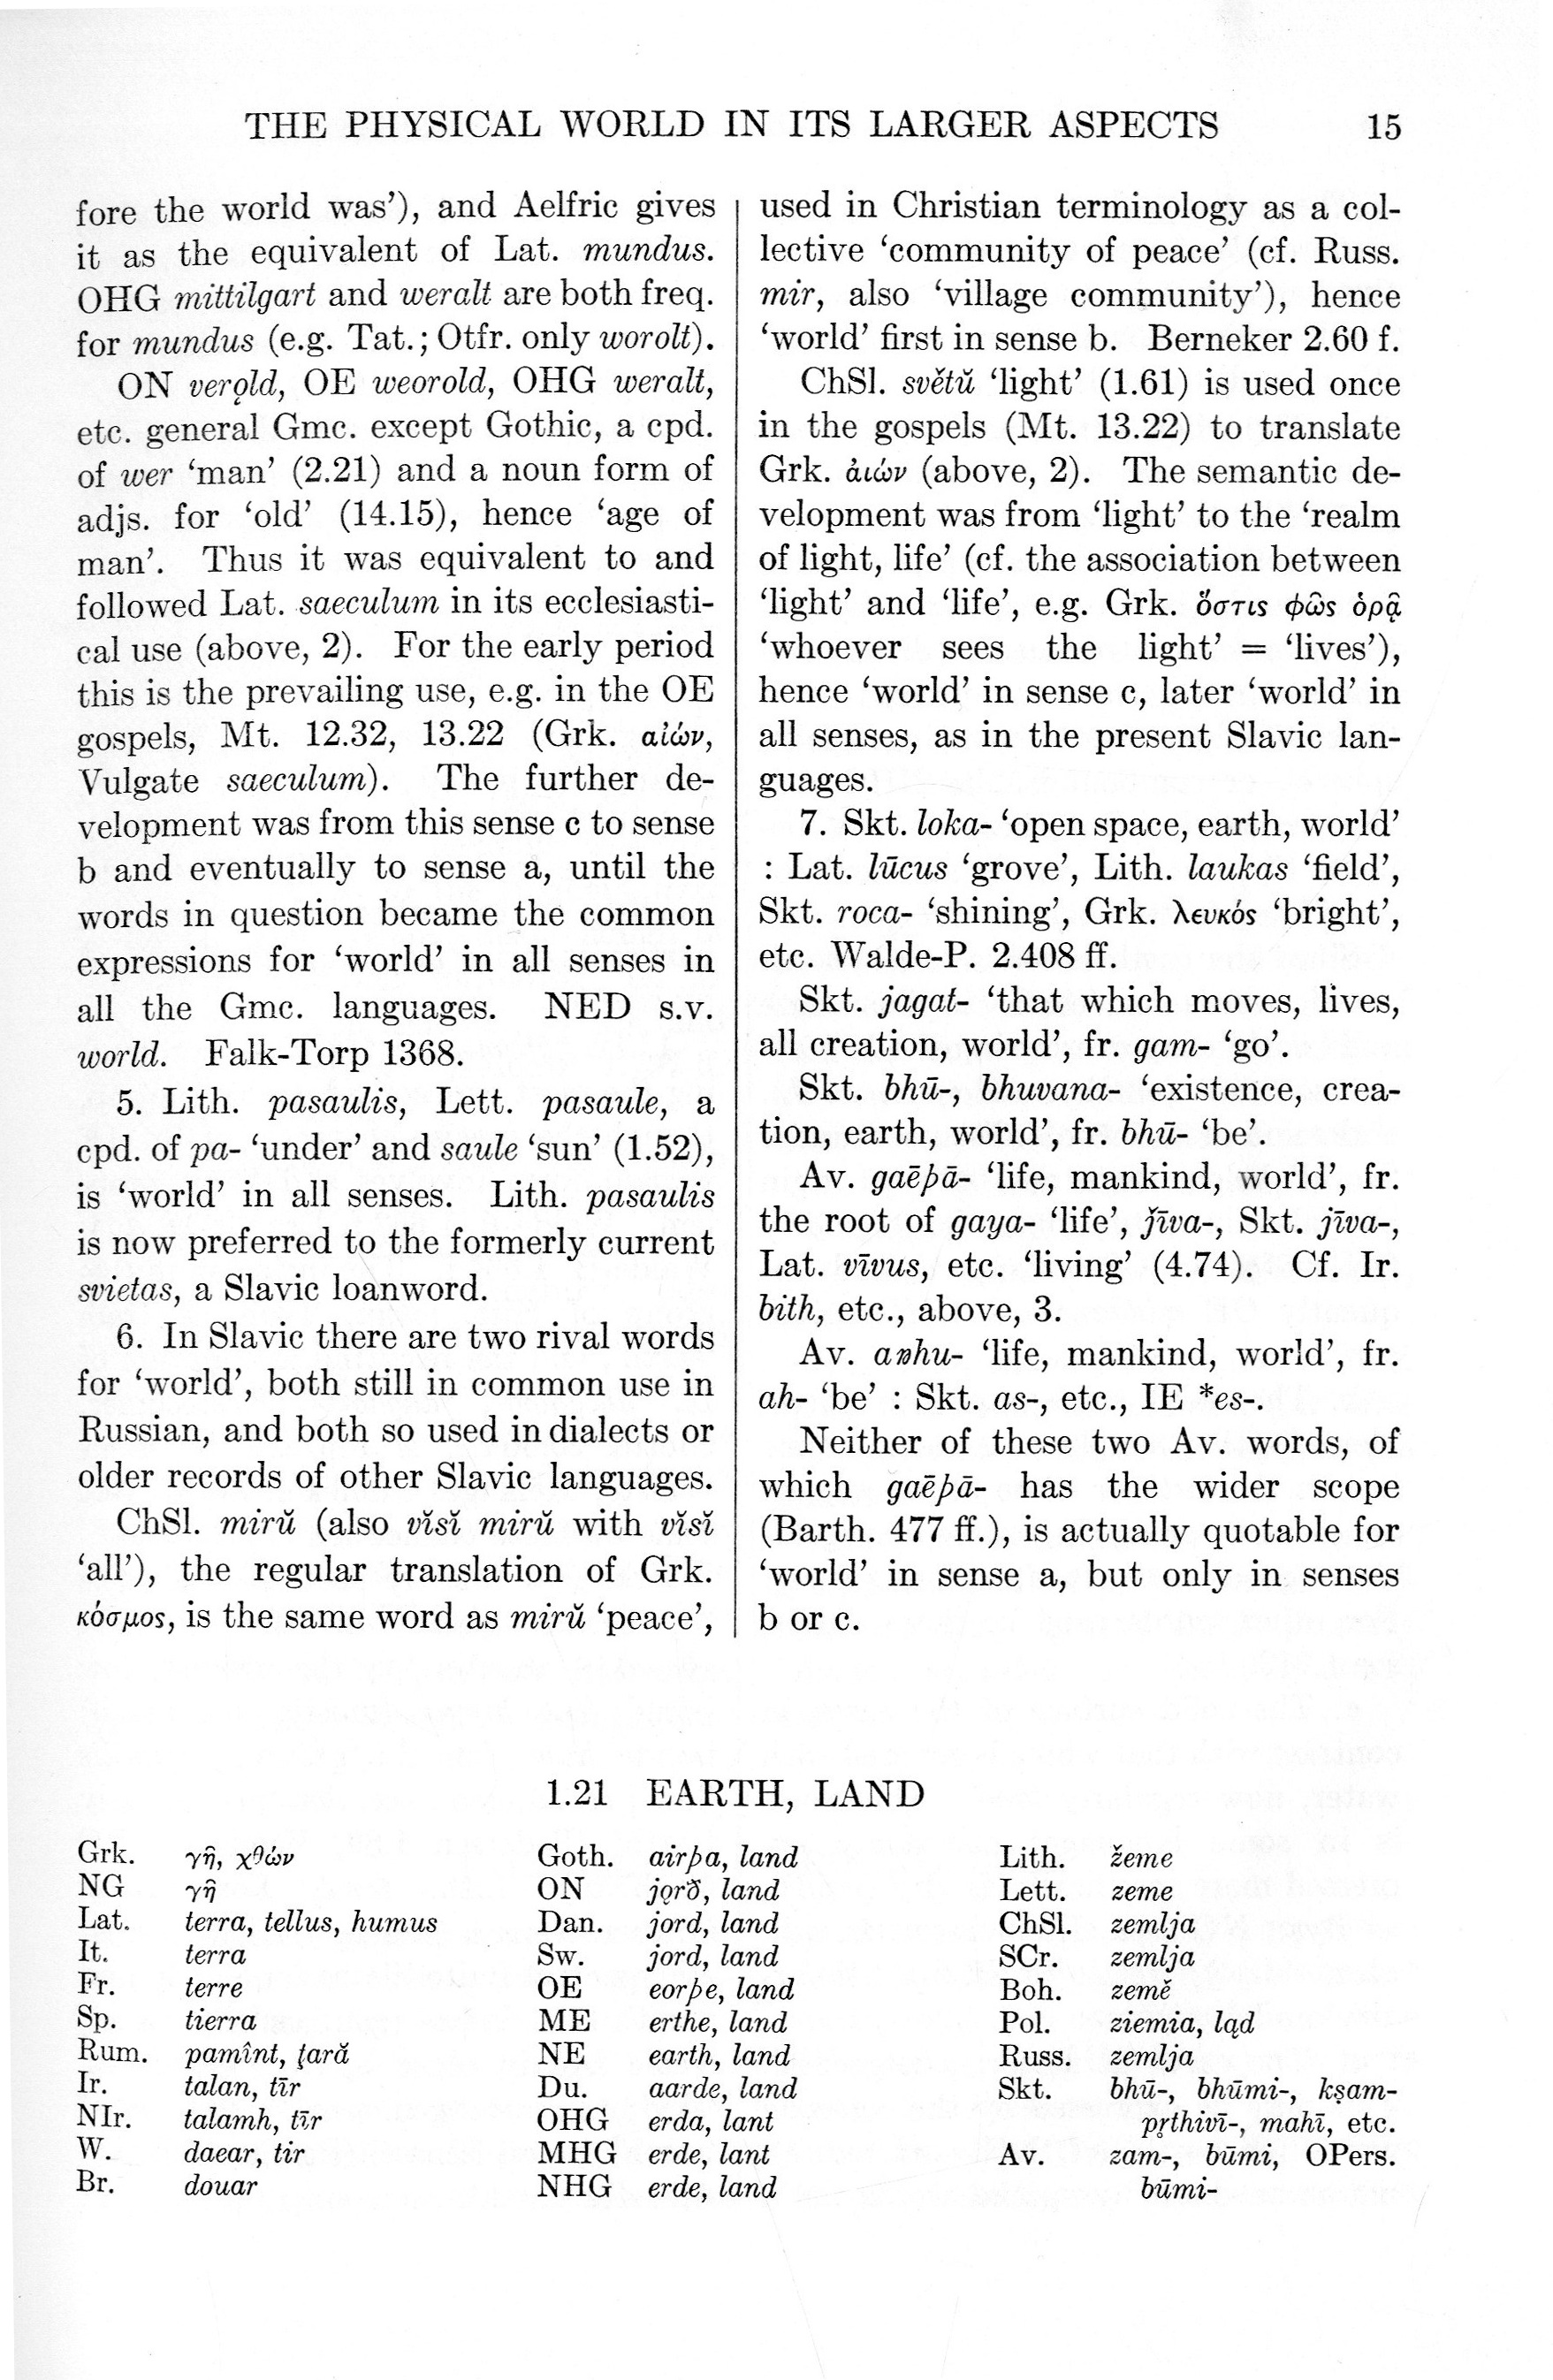
\includegraphics[width=\linewidth]{Stolk_thes-content/fig/thes/DSSPIEL-p0015.jpg}
    \caption{\textit{DSSPIEL} thesaurus, p. 15.}
  \label{fig:1.A:DSSPIEL:thesaurus}
\end{figure}

\begin{figure}[htbp]
  \centering
    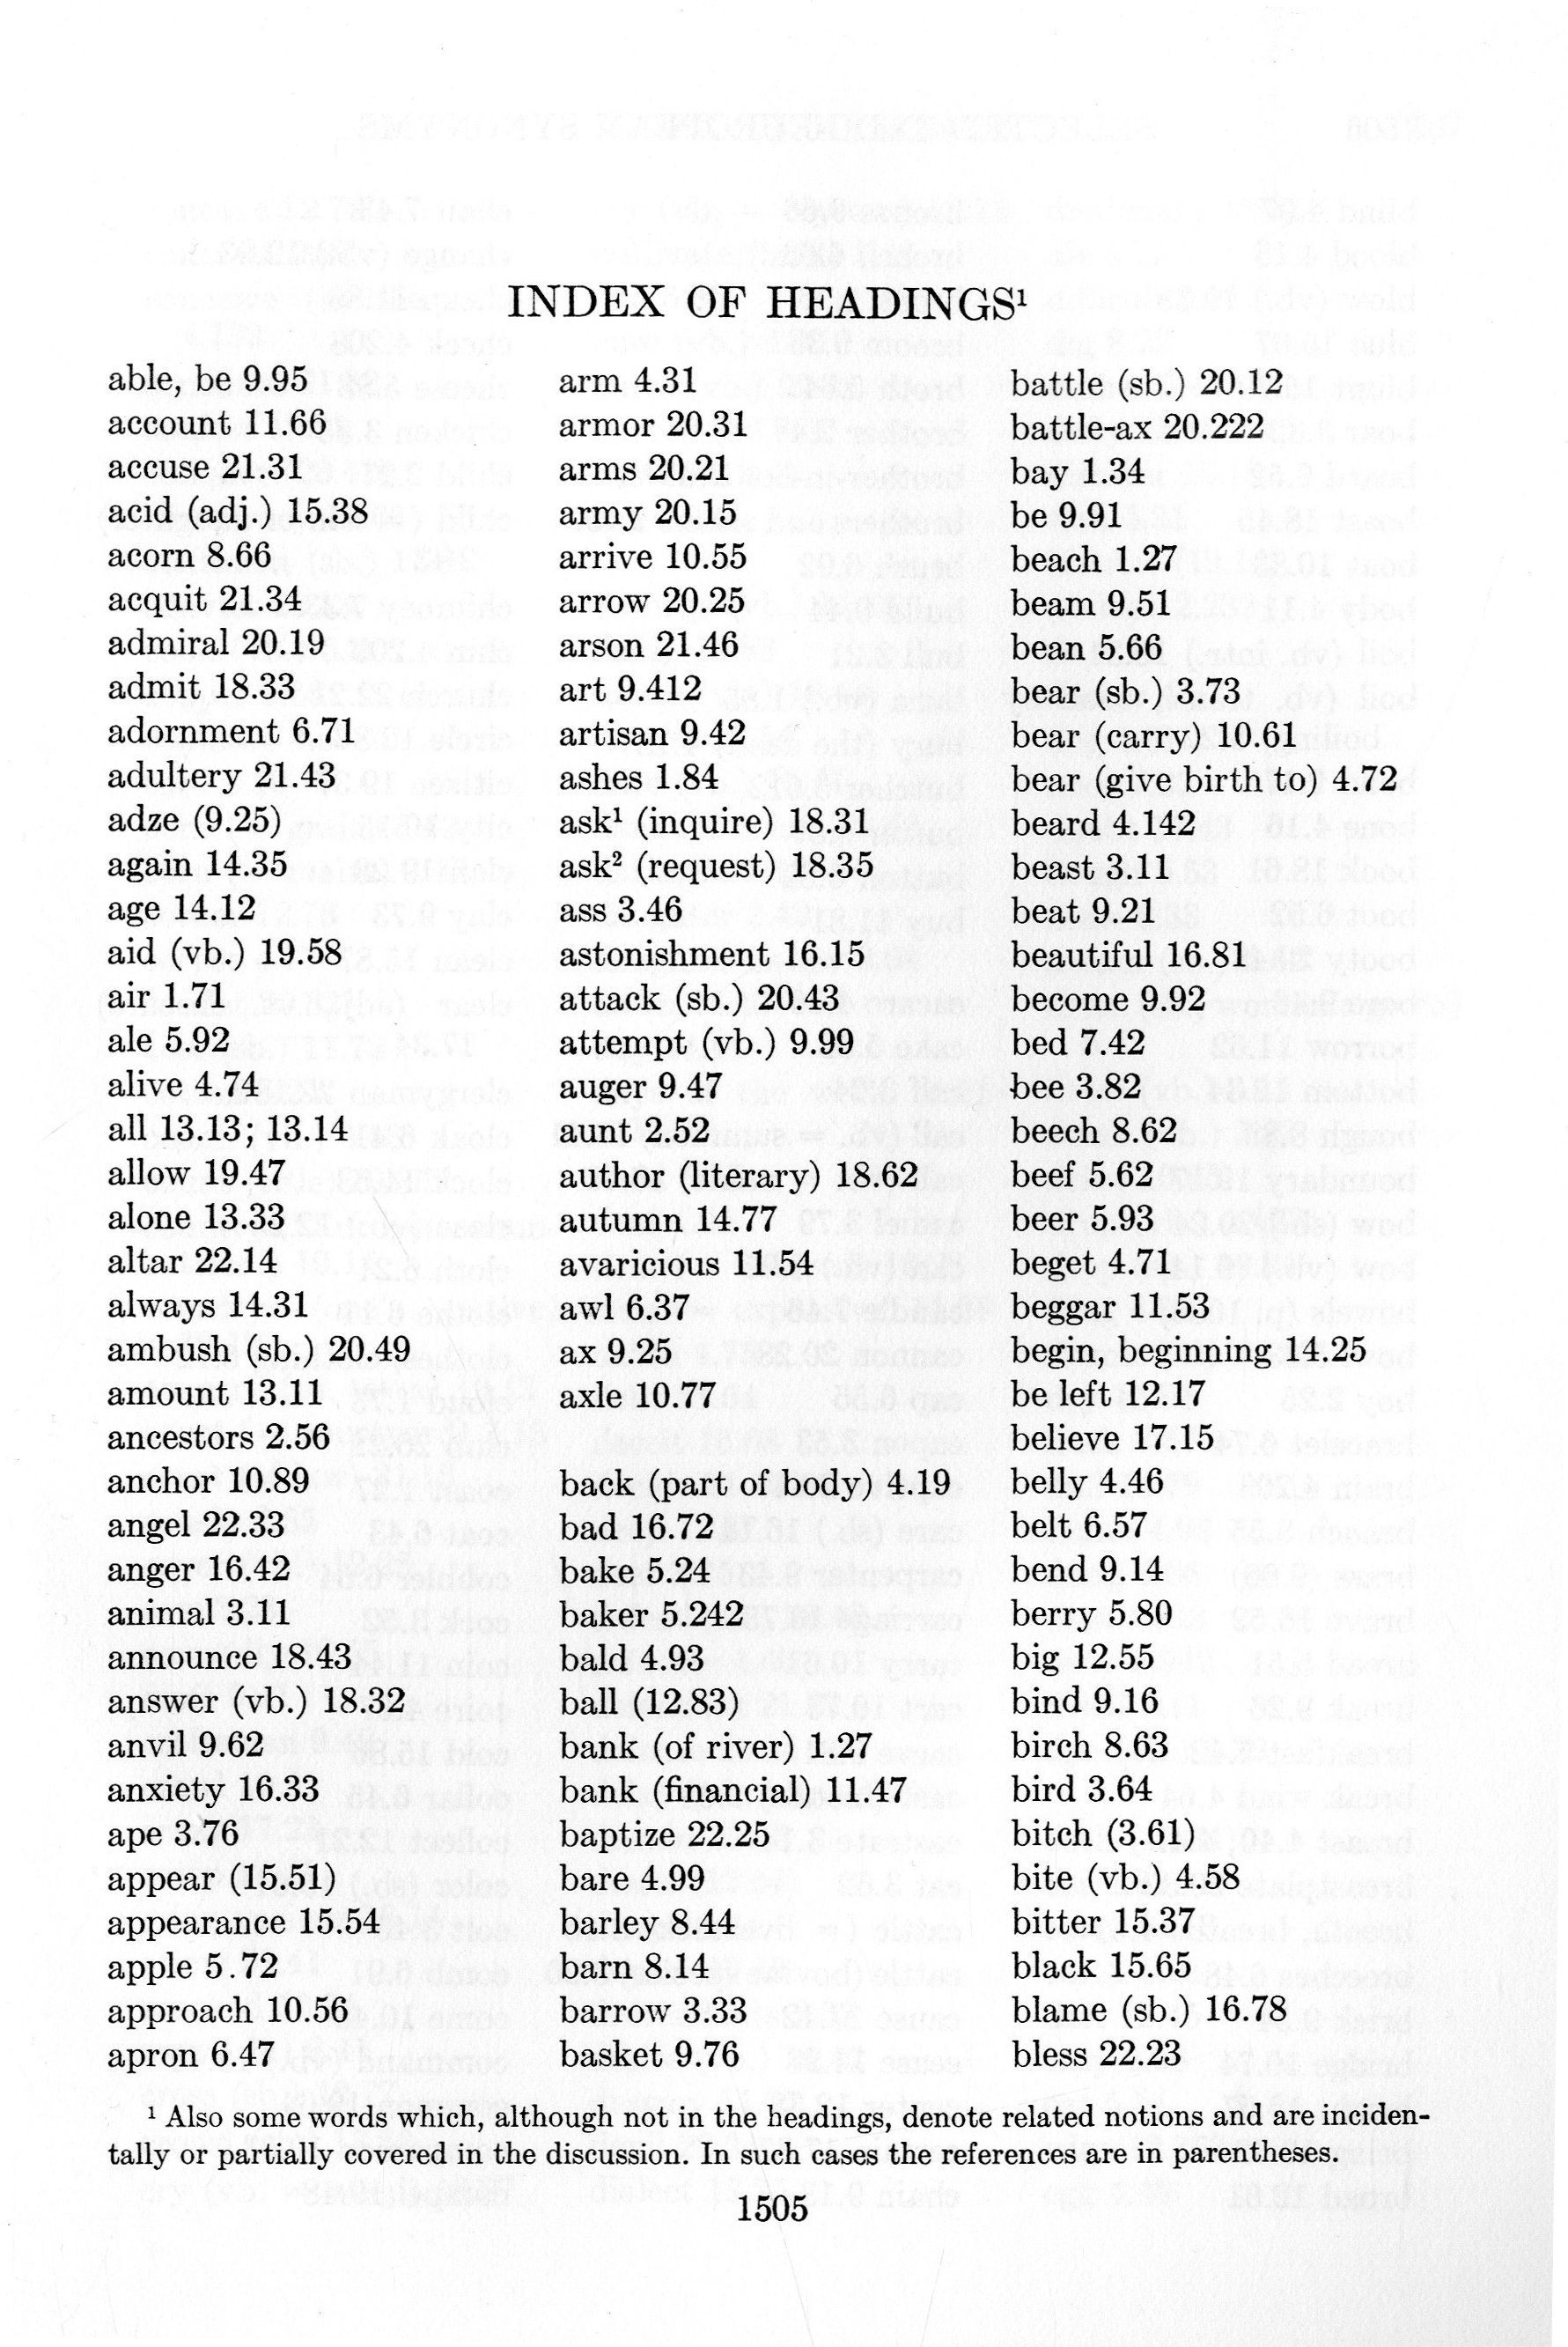
\includegraphics[width=\linewidth]{Stolk_thes-content/fig/thes/DSSPIEL-p1505.jpg}
    \caption{\textit{DSSPIEL} index, p. 1505.}
  \label{fig:1.A:DSSPIEL:index}
\end{figure}

%% ScT

\begin{figure}[htbp]
  \centering
    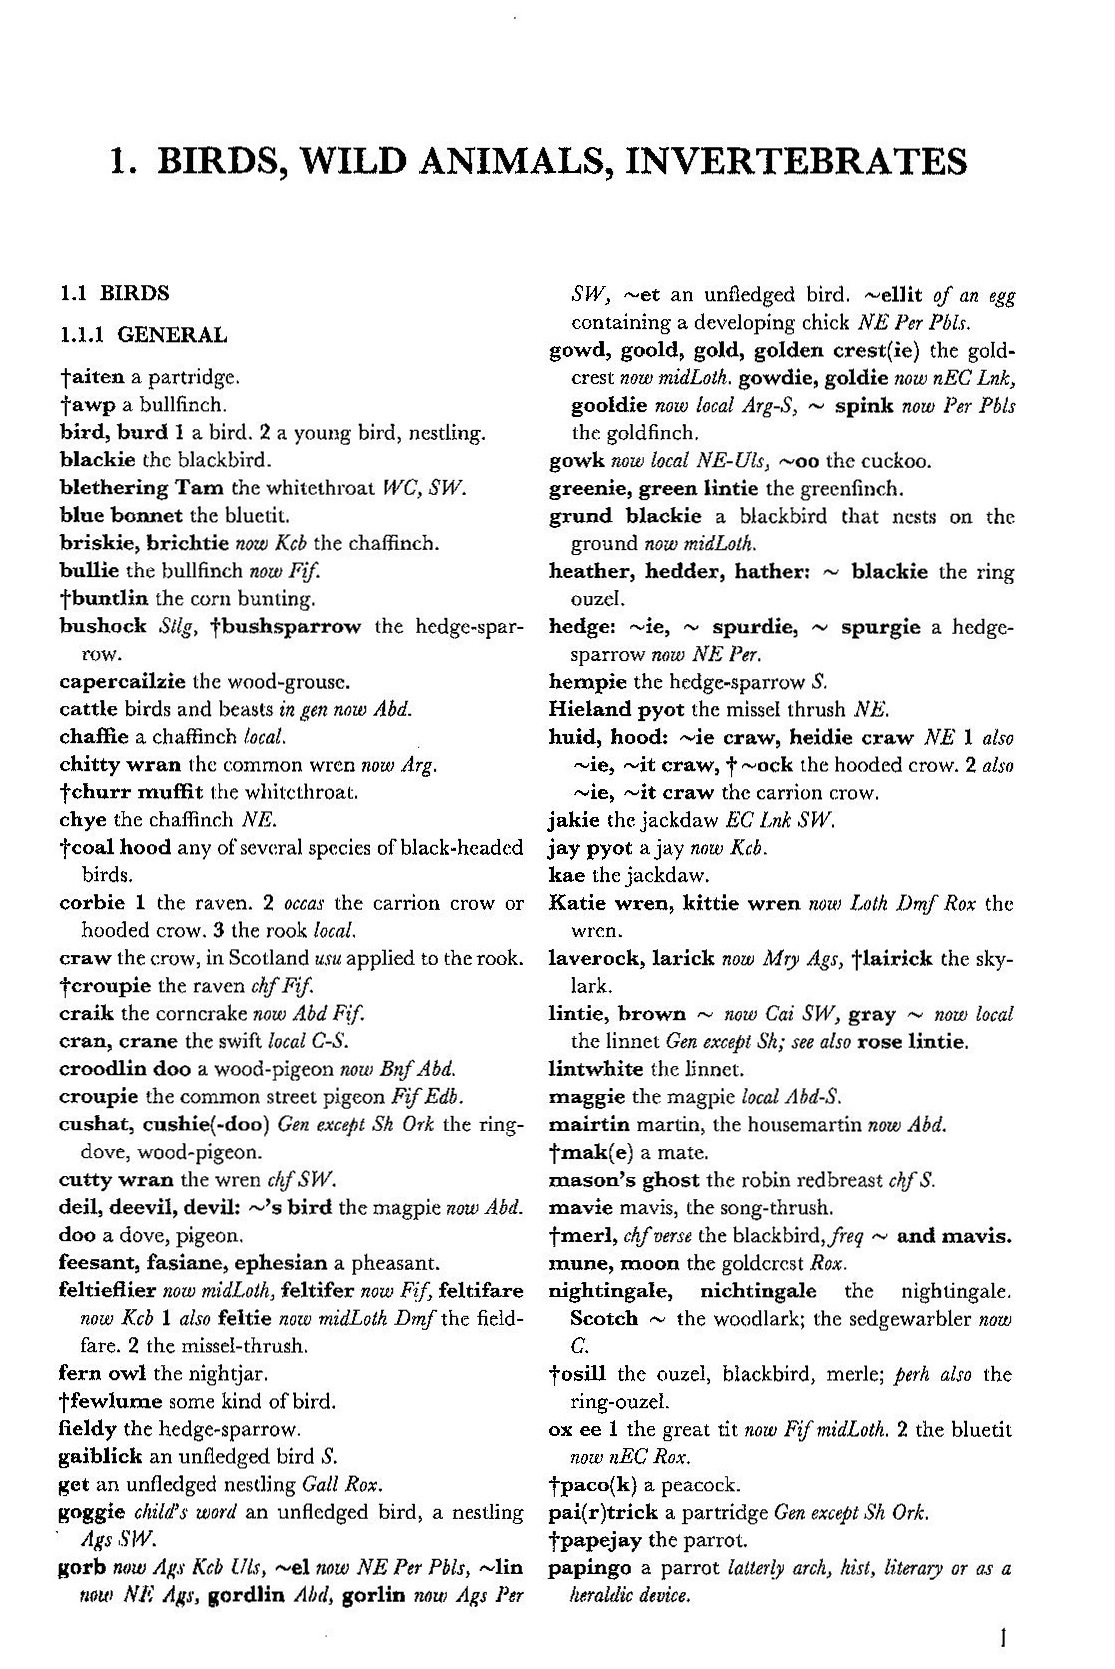
\includegraphics[width=\linewidth]{Stolk_thes-content/fig/thes/ScT-p001.jpg}
  \caption{\textit{ScT} thesaurus, p. 1.}
  \label{fig:1.A:ScT:thesaurus}
\end{figure}

\begin{figure}[htbp]
  \centering
    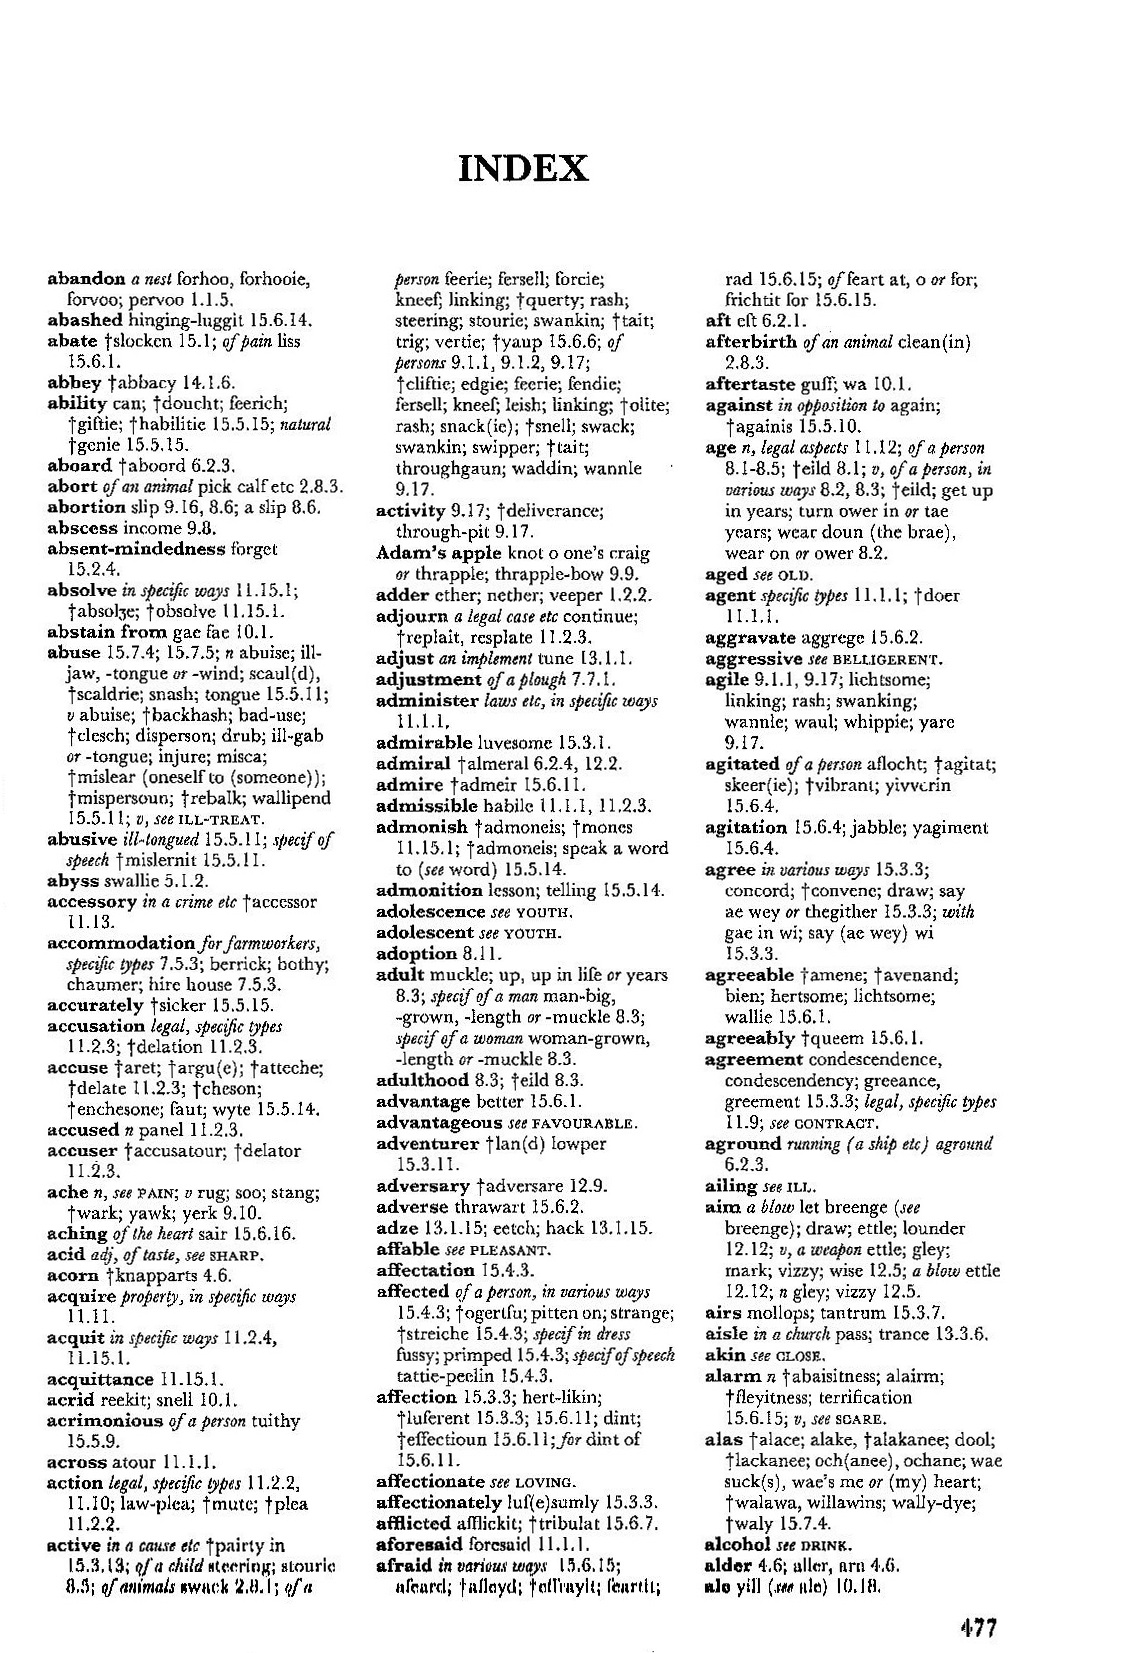
\includegraphics[width=\linewidth]{Stolk_thes-content/fig/thes/ScT-p477.jpg}
  \caption{\textit{ScT} index, p. 477.}
  \label{fig:1.A:ScT:index}
\end{figure}

%% ShT

\begin{figure}[htbp]
  \centering
    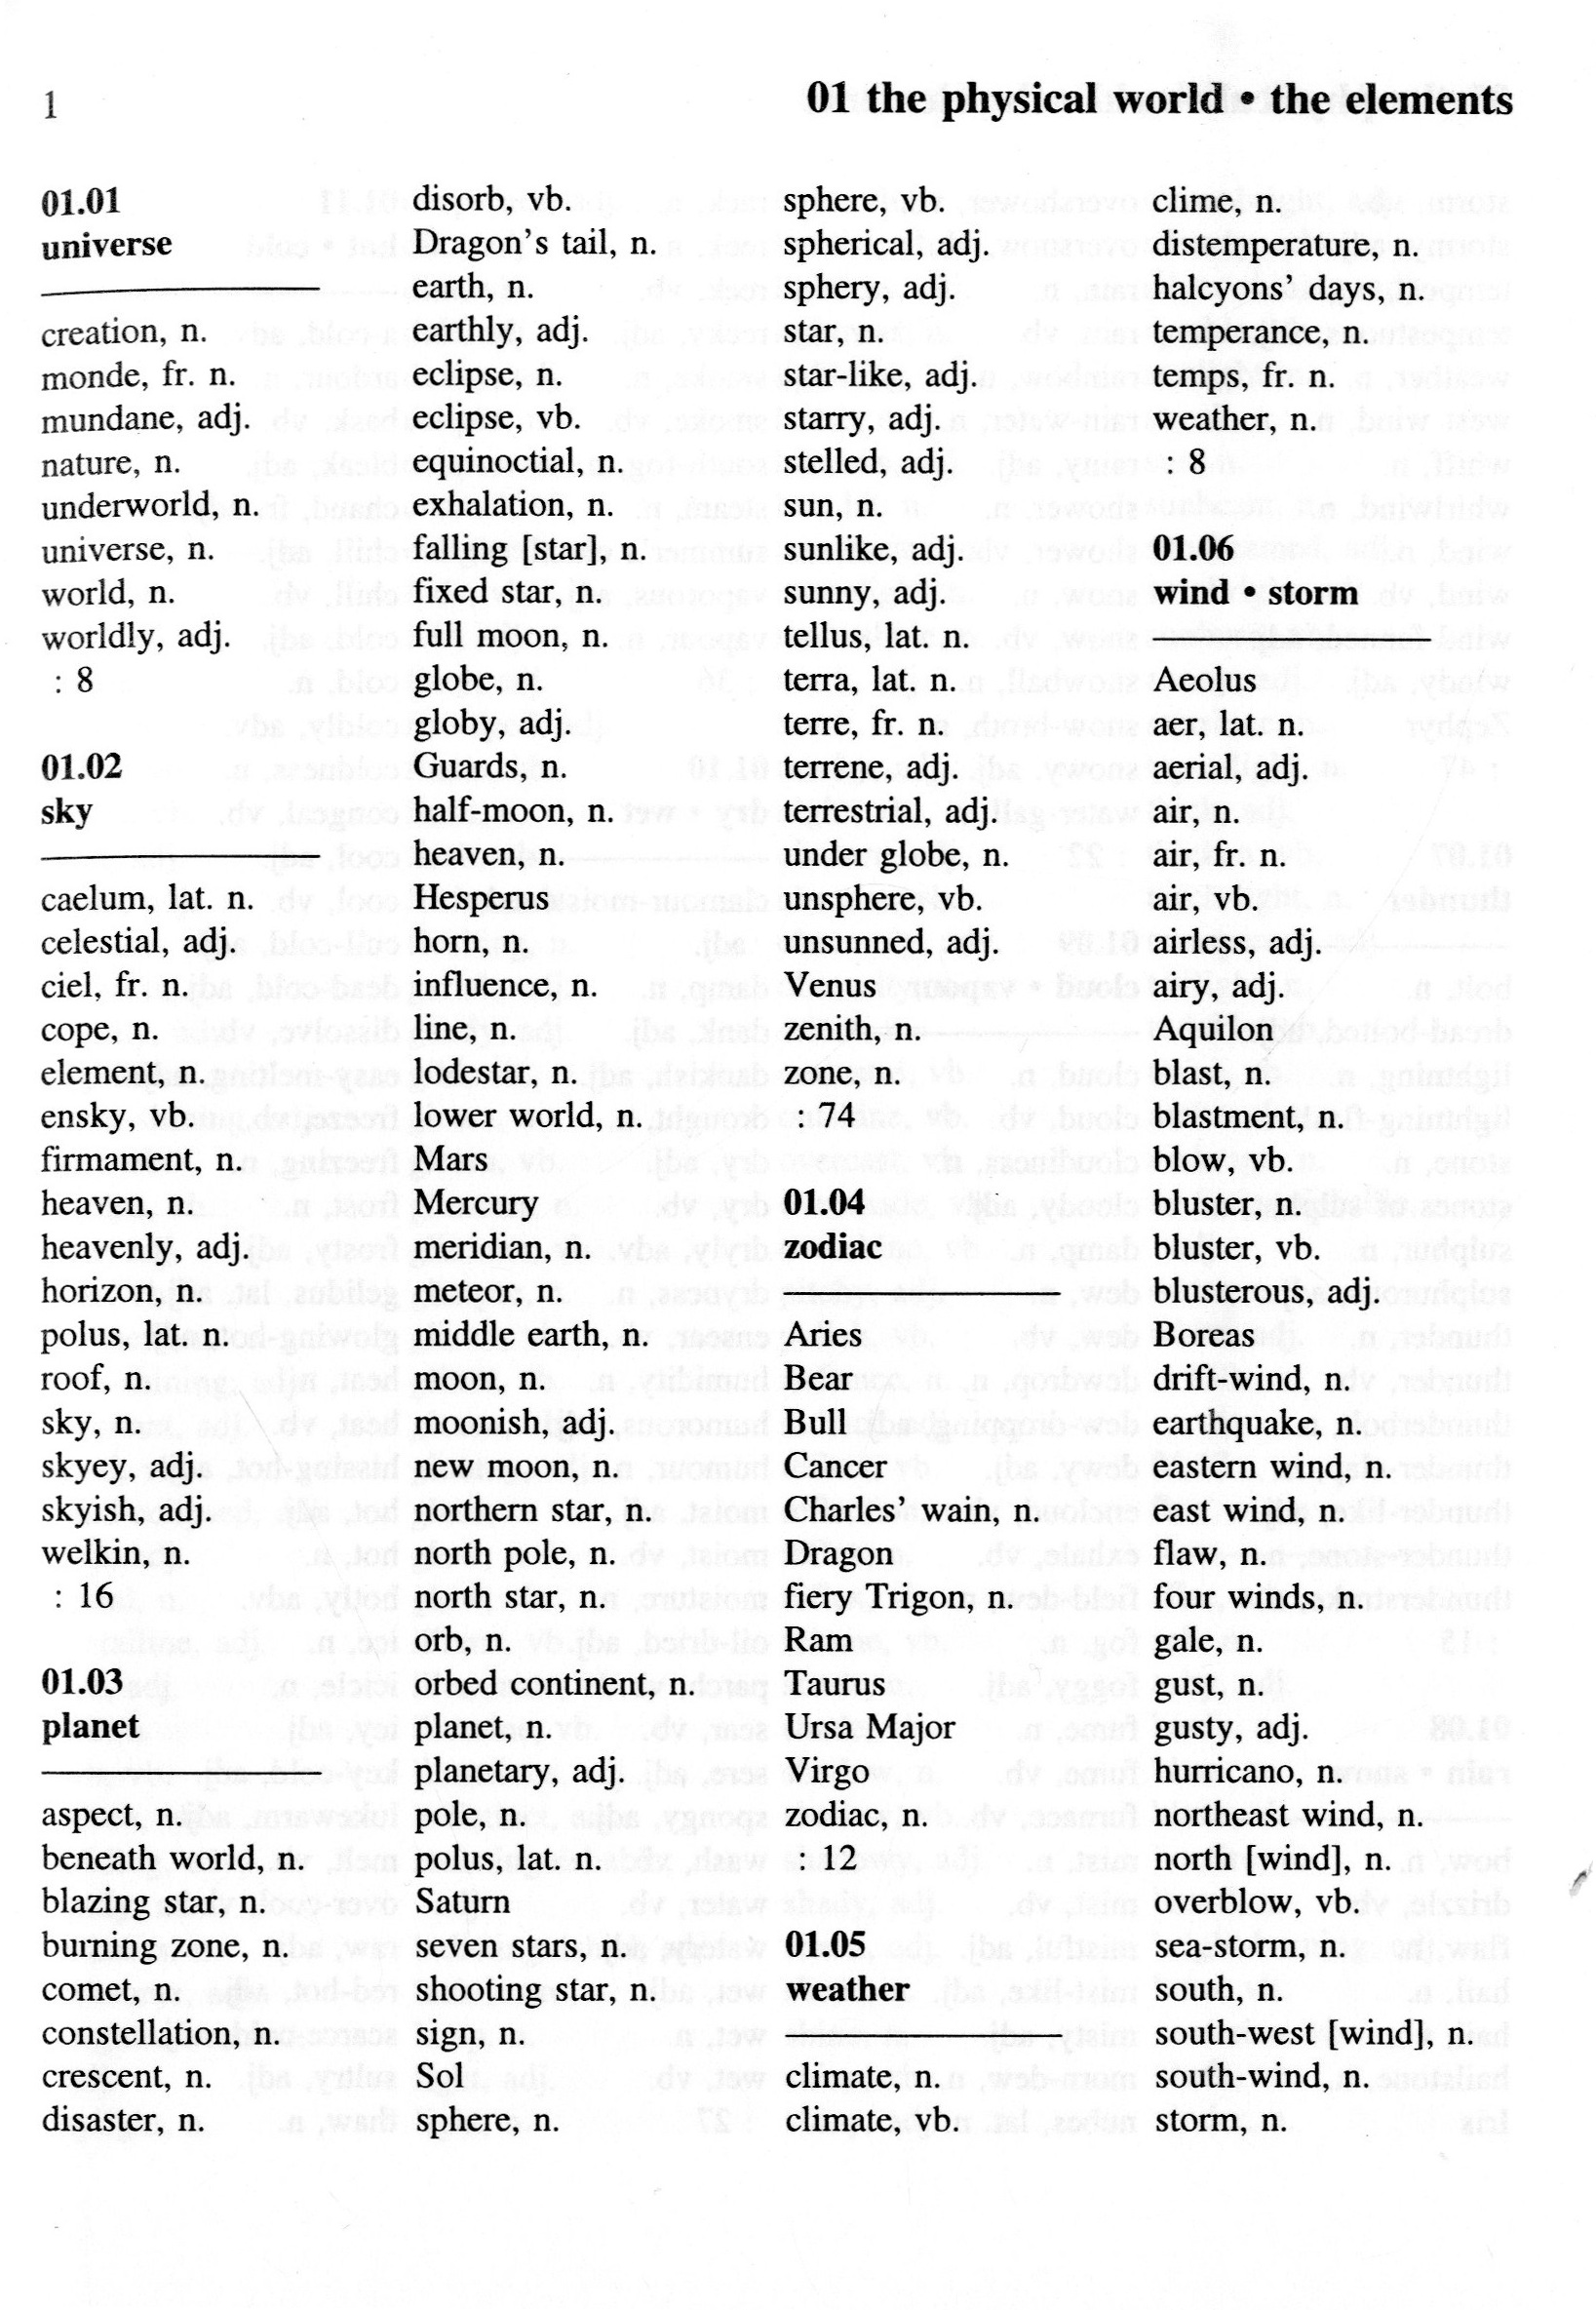
\includegraphics[width=\linewidth]{Stolk_thes-content/fig/thes/ShT-p001.jpg}
  \caption{\textit{ShT} thesaurus, p. 1.}
  \label{fig:1.A:ShT:thesaurus}
\end{figure}

\begin{figure}[htbp]
  \centering
    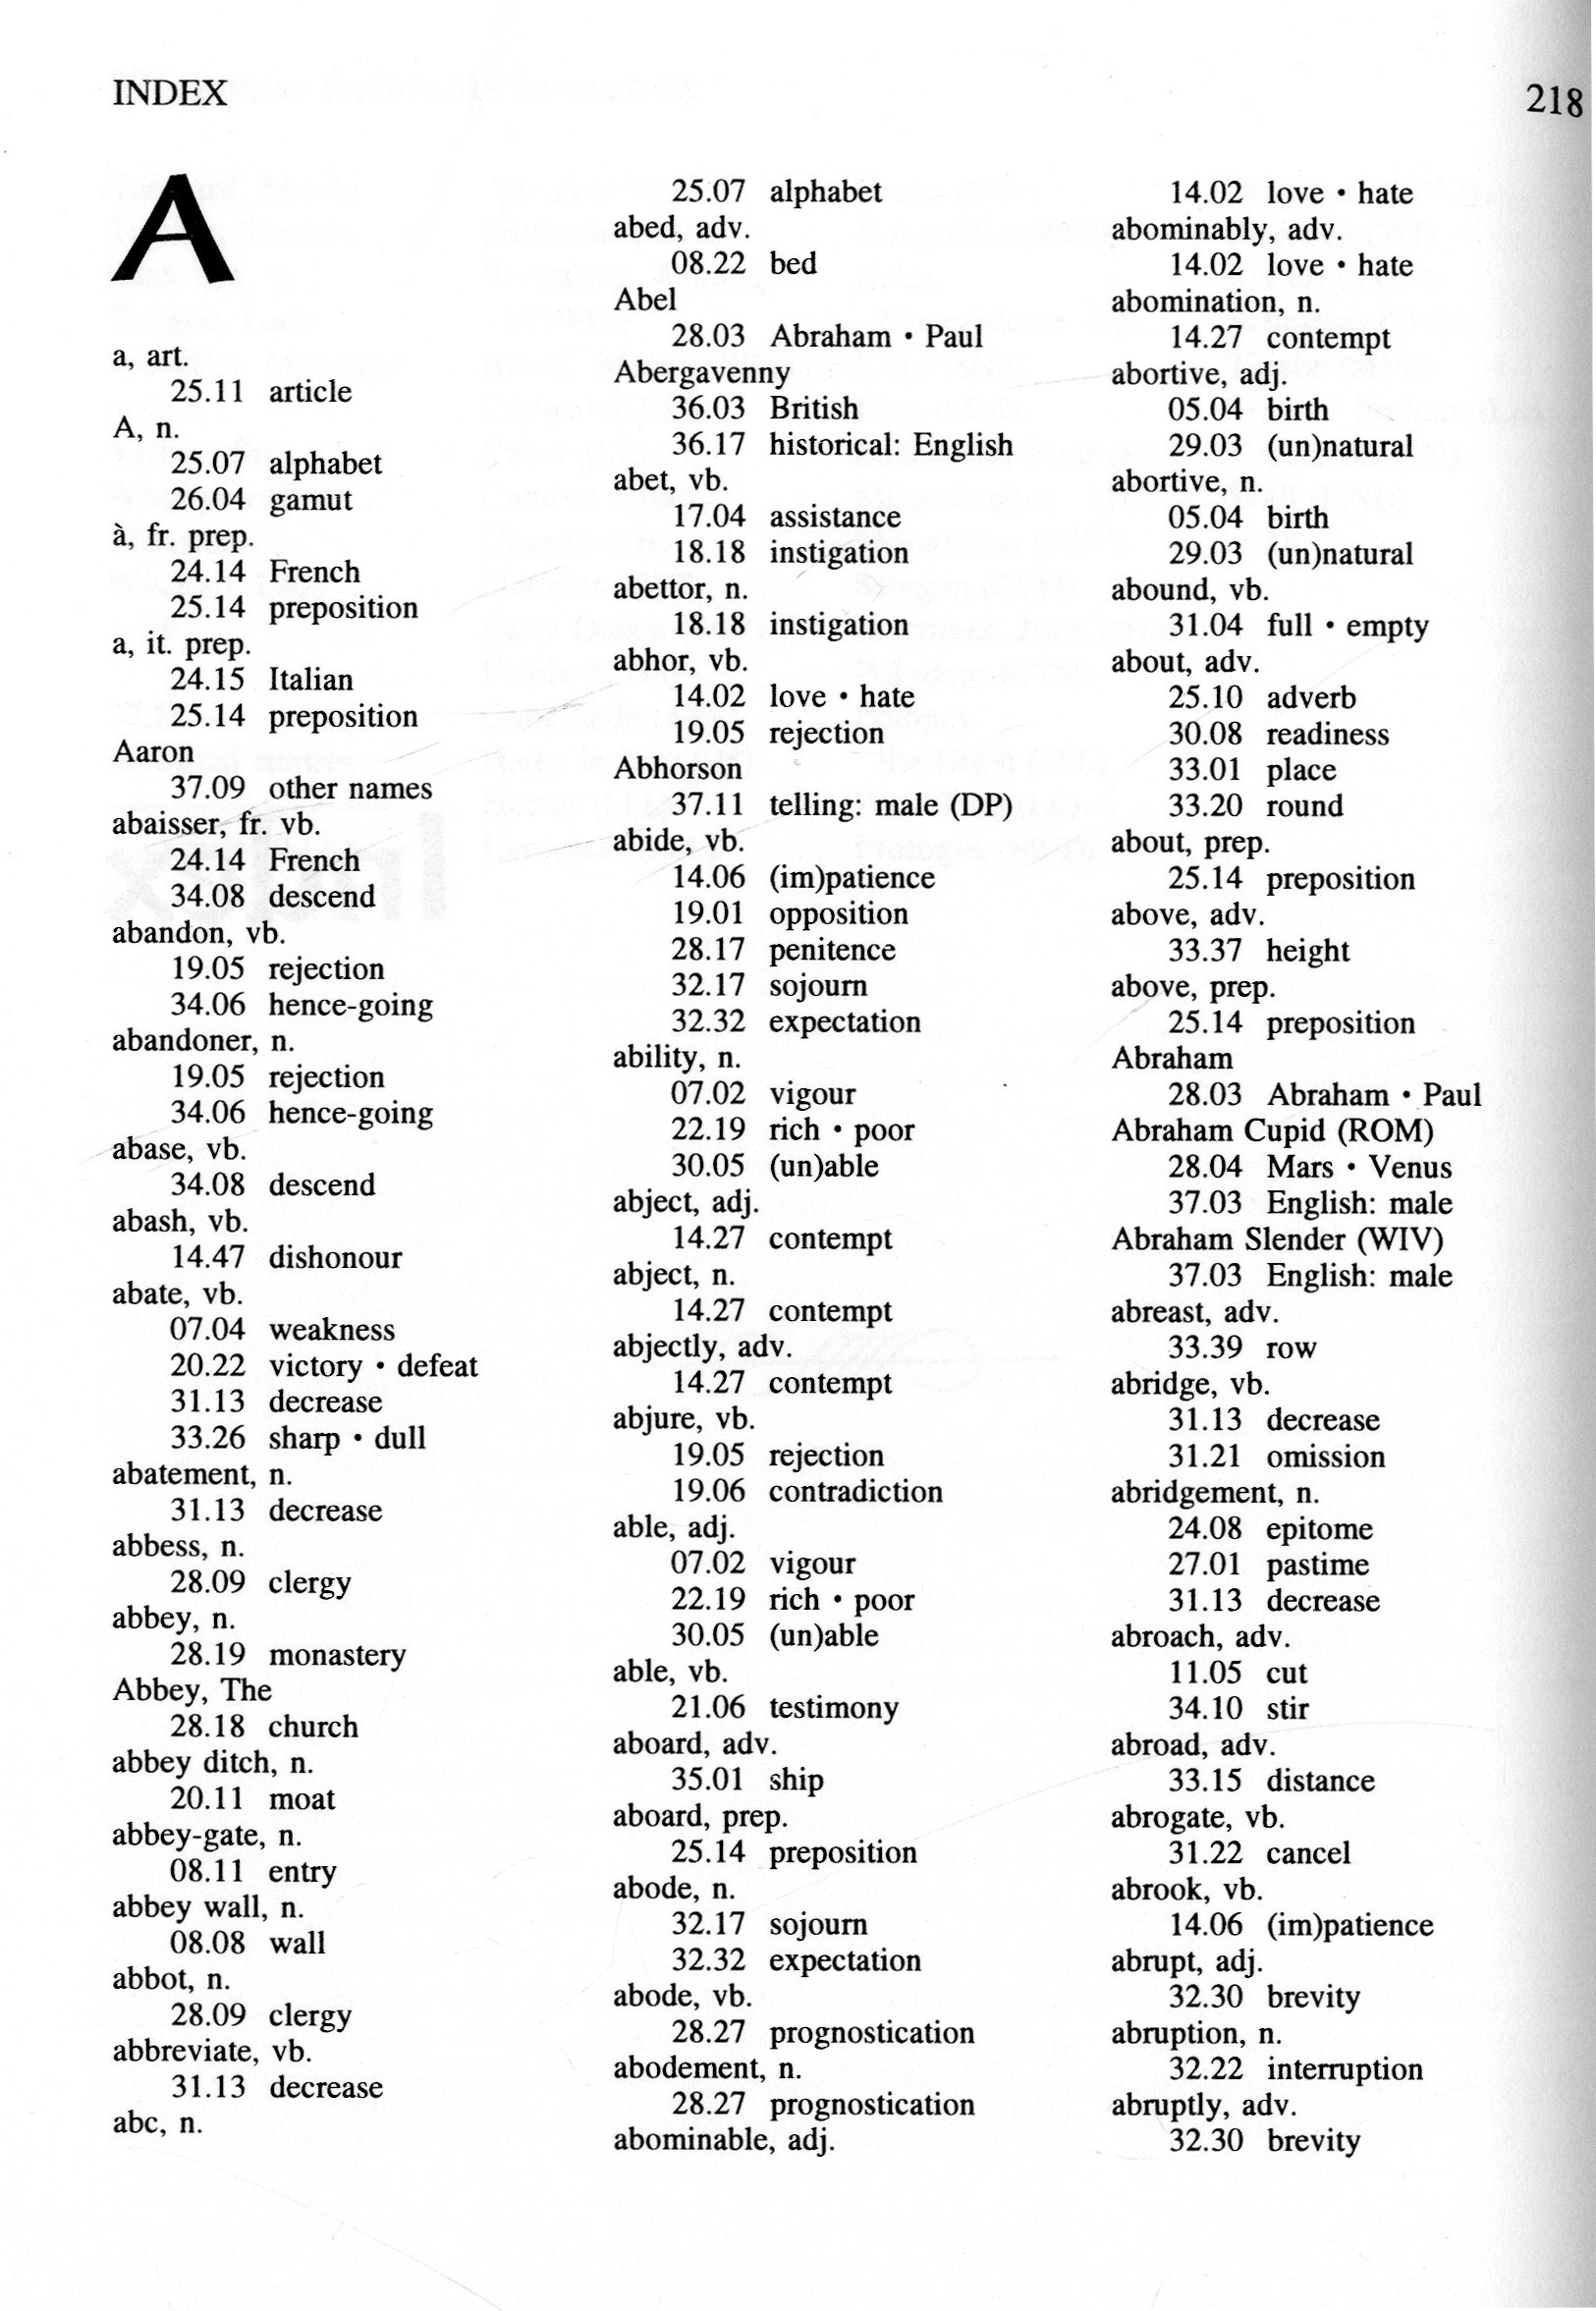
\includegraphics[width=\linewidth]{Stolk_thes-content/fig/thes/ShT-p218.jpg}
  \caption{\textit{ShT} index, p. 218.}
  \label{fig:1.A:ShT:index}
\end{figure}

%% TOE2

\begin{figure}[htbp]
  \centering
    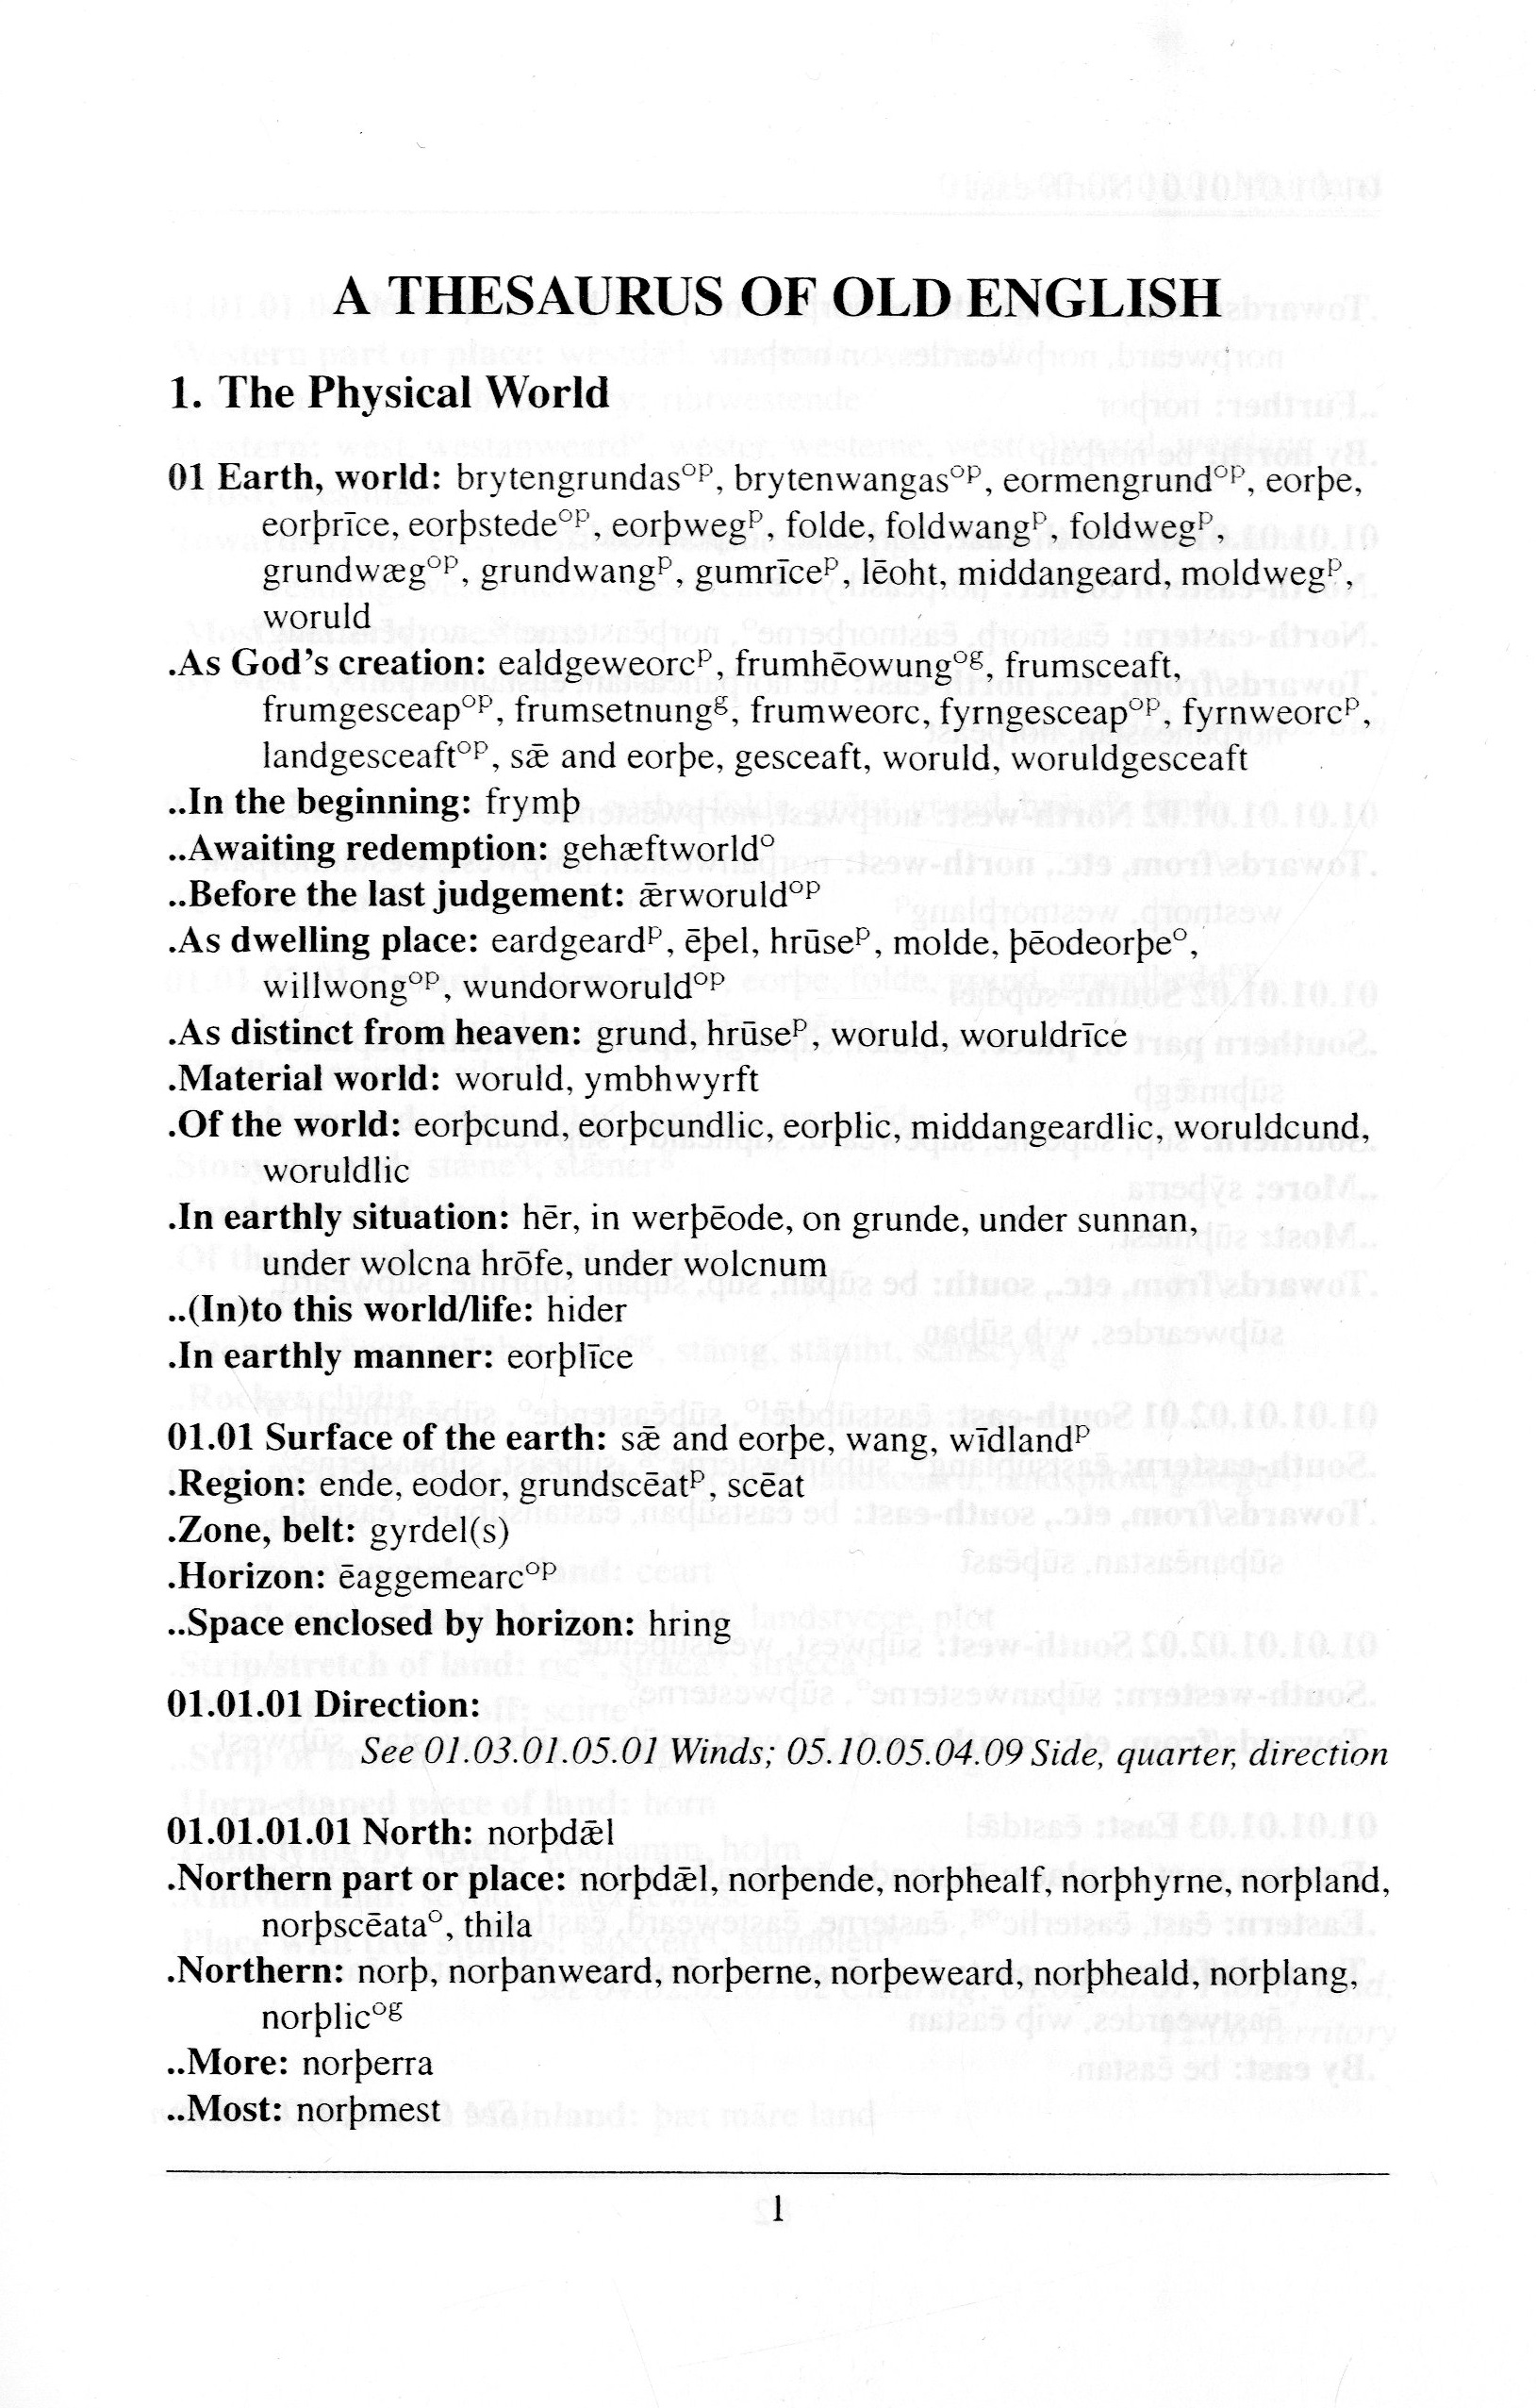
\includegraphics[width=\linewidth]{Stolk_thes-content/fig/thes/TOE2-p001.jpg}
  \caption{\textit{TOE2} thesaurus, p. 1.}
  \label{fig:1.A:TOE2:thesaurus}
\end{figure}

\begin{figure}[htbp]
  \centering
    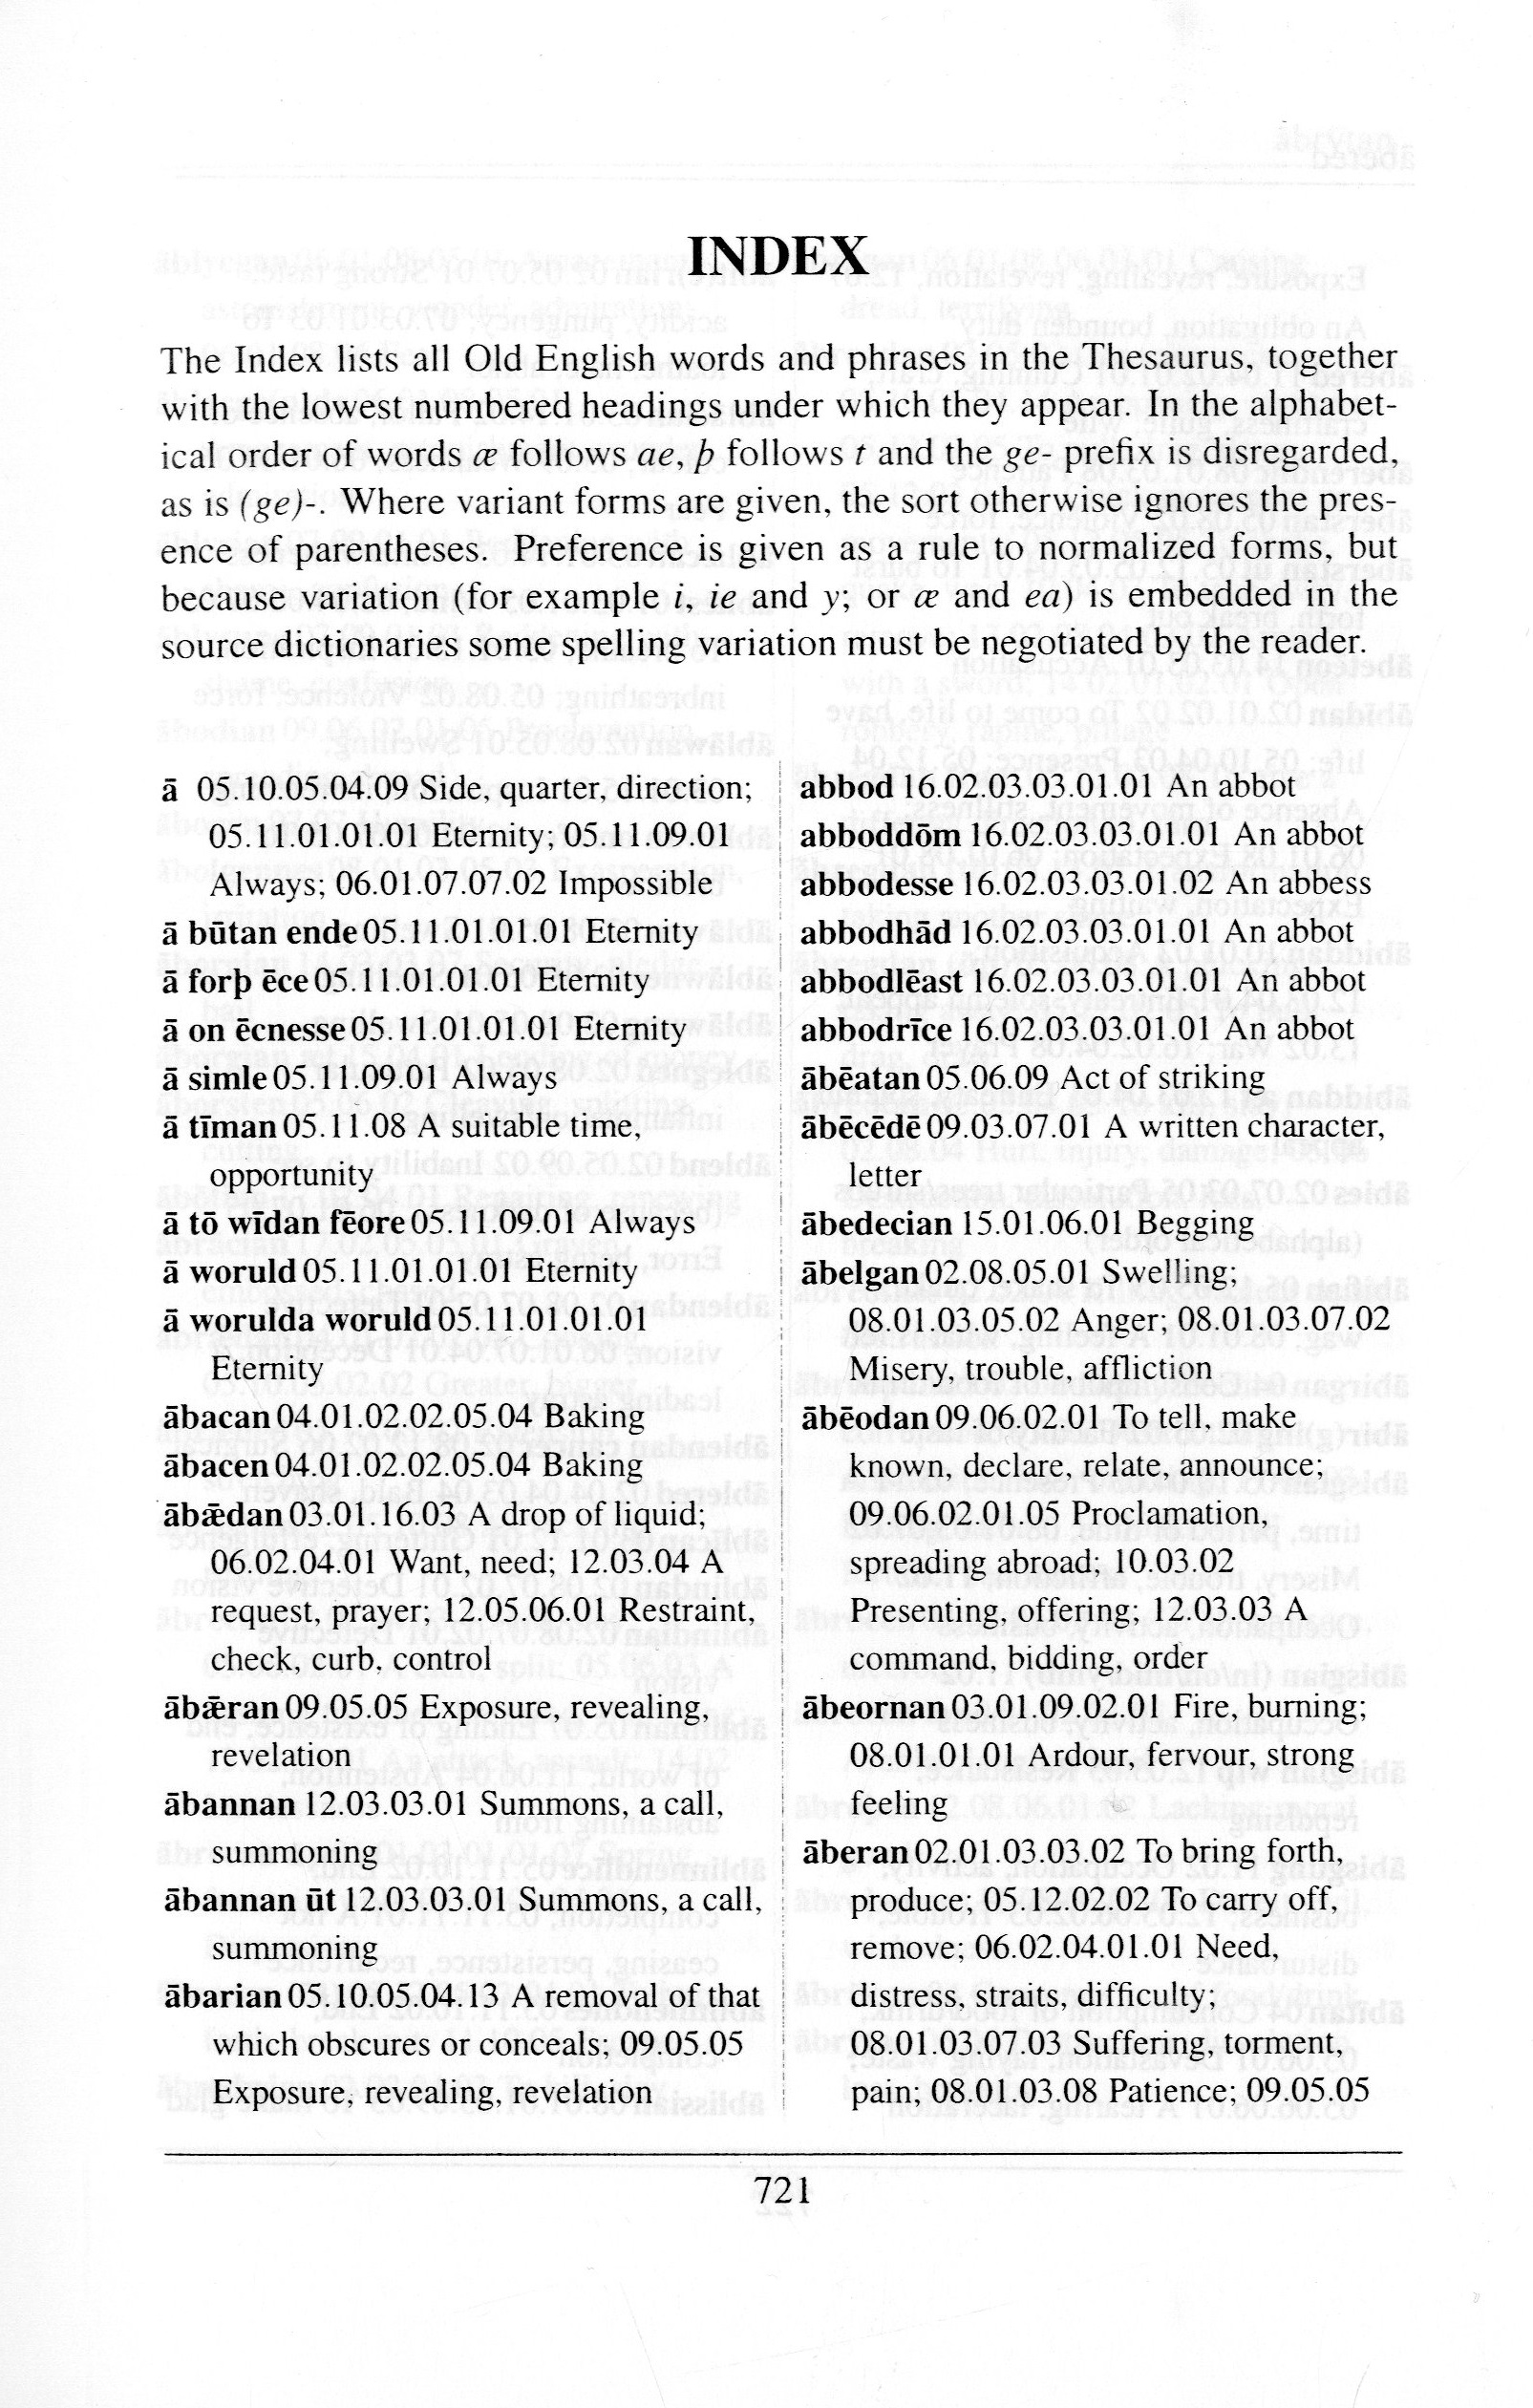
\includegraphics[width=\linewidth]{Stolk_thes-content/fig/thes/TOE2-p721.jpg}
  \caption{\textit{TOE2} index, p. 721.}
  \label{fig:1.A:TOE2:index}
\end{figure}


%% TOE4

\begin{figure}[htbp]
  \centering
    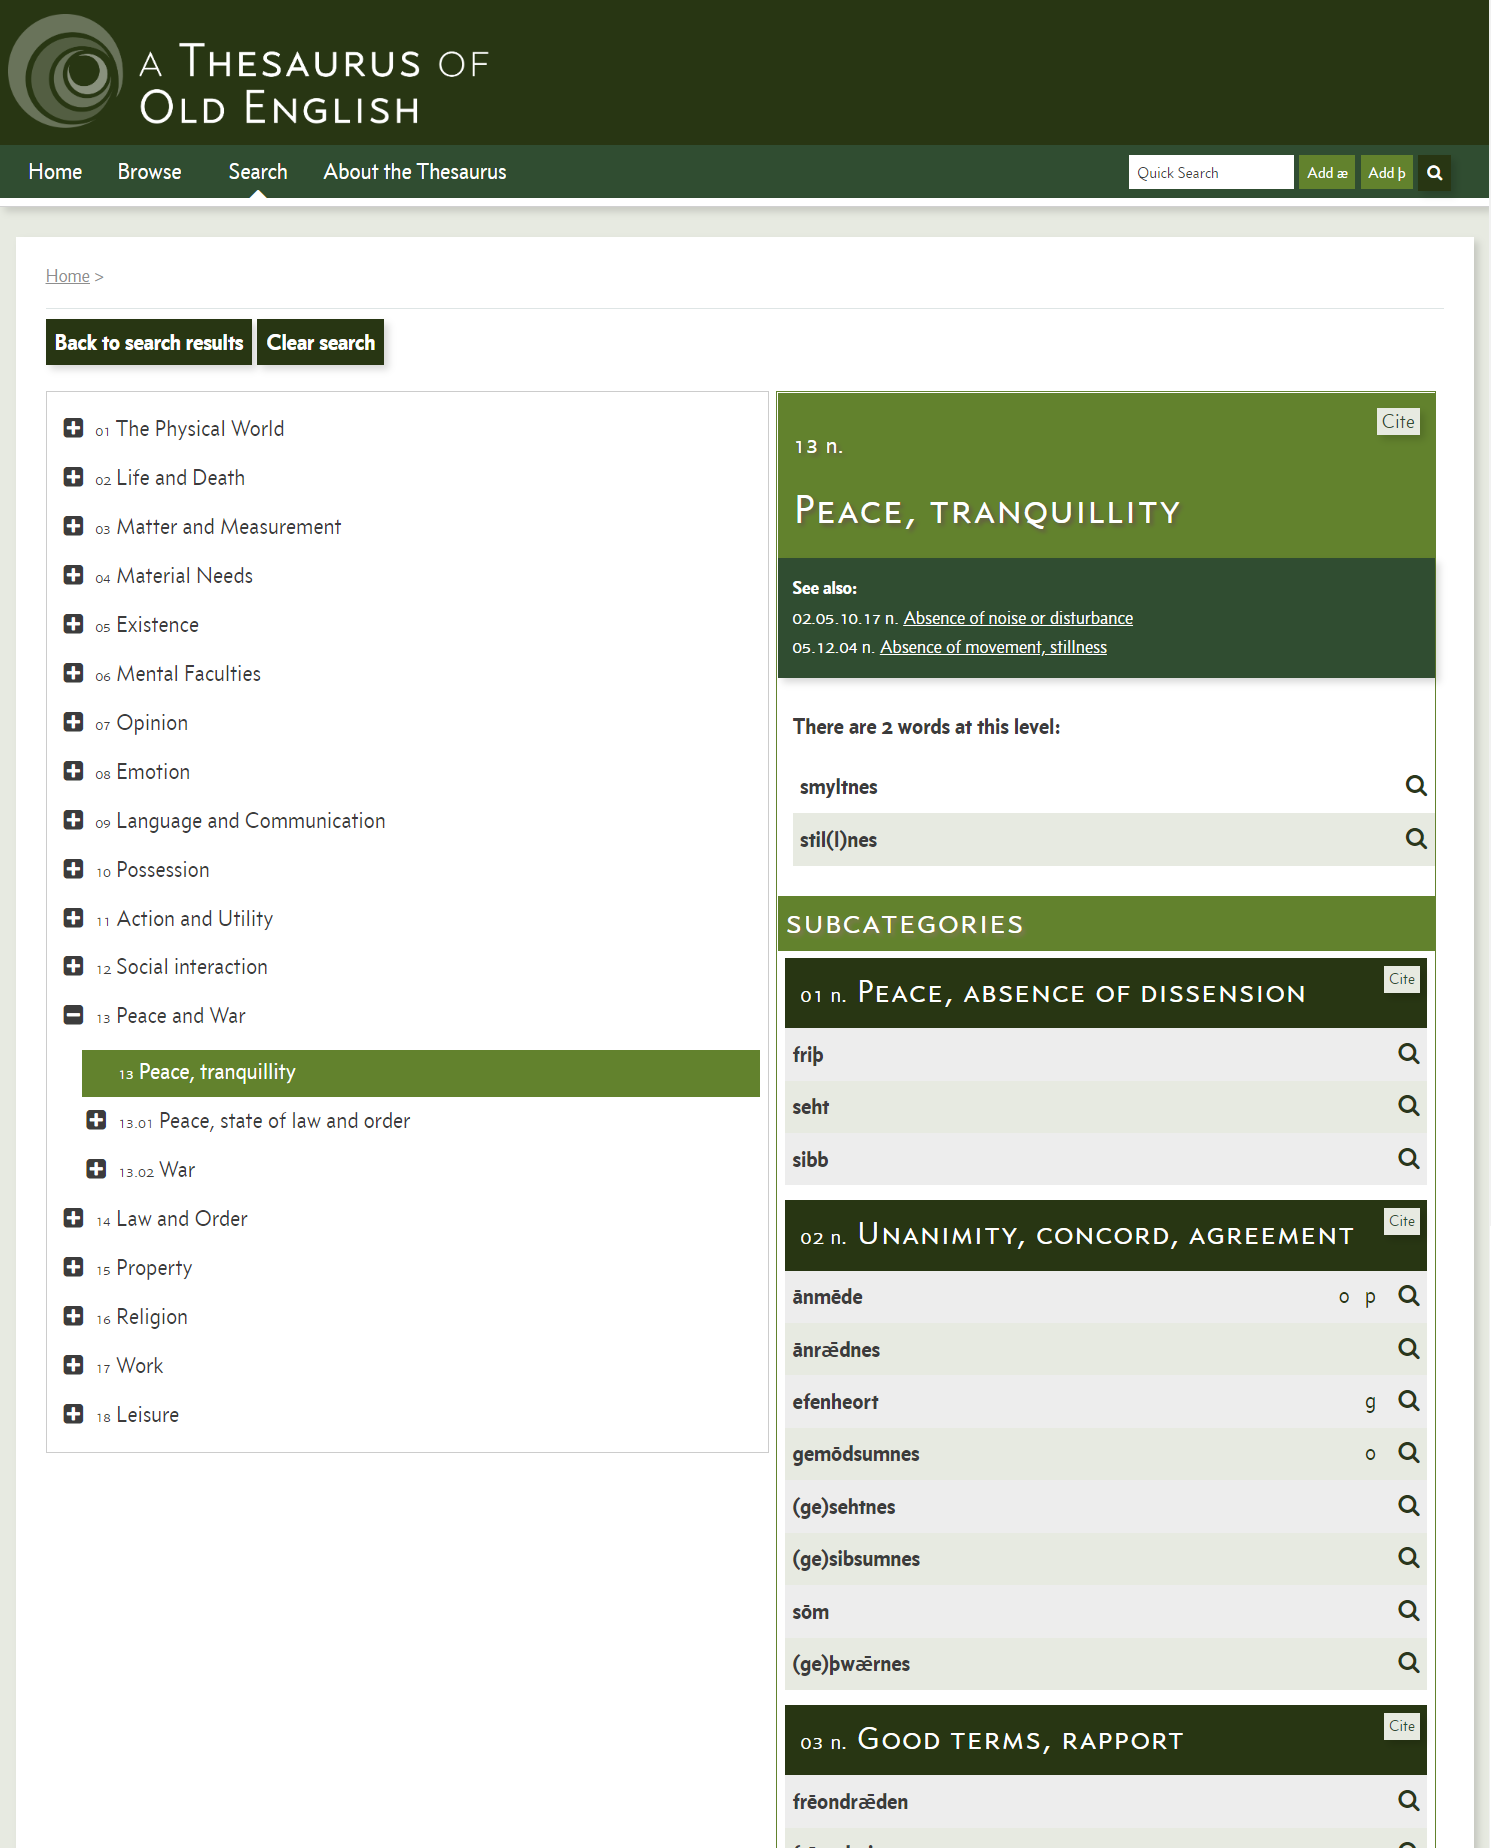
\includegraphics[width=\linewidth]{Stolk_thes-content/fig/thes/TOE4-thesaurus-peacetranquility.png}
  \caption{\textit{TOE4} thesaurus, category ``13 n. Peace, tranquility''.}
  \label{fig:1.A:TOE4:thesaurus}
\end{figure}

\begin{figure}[htbp]
  \centering
    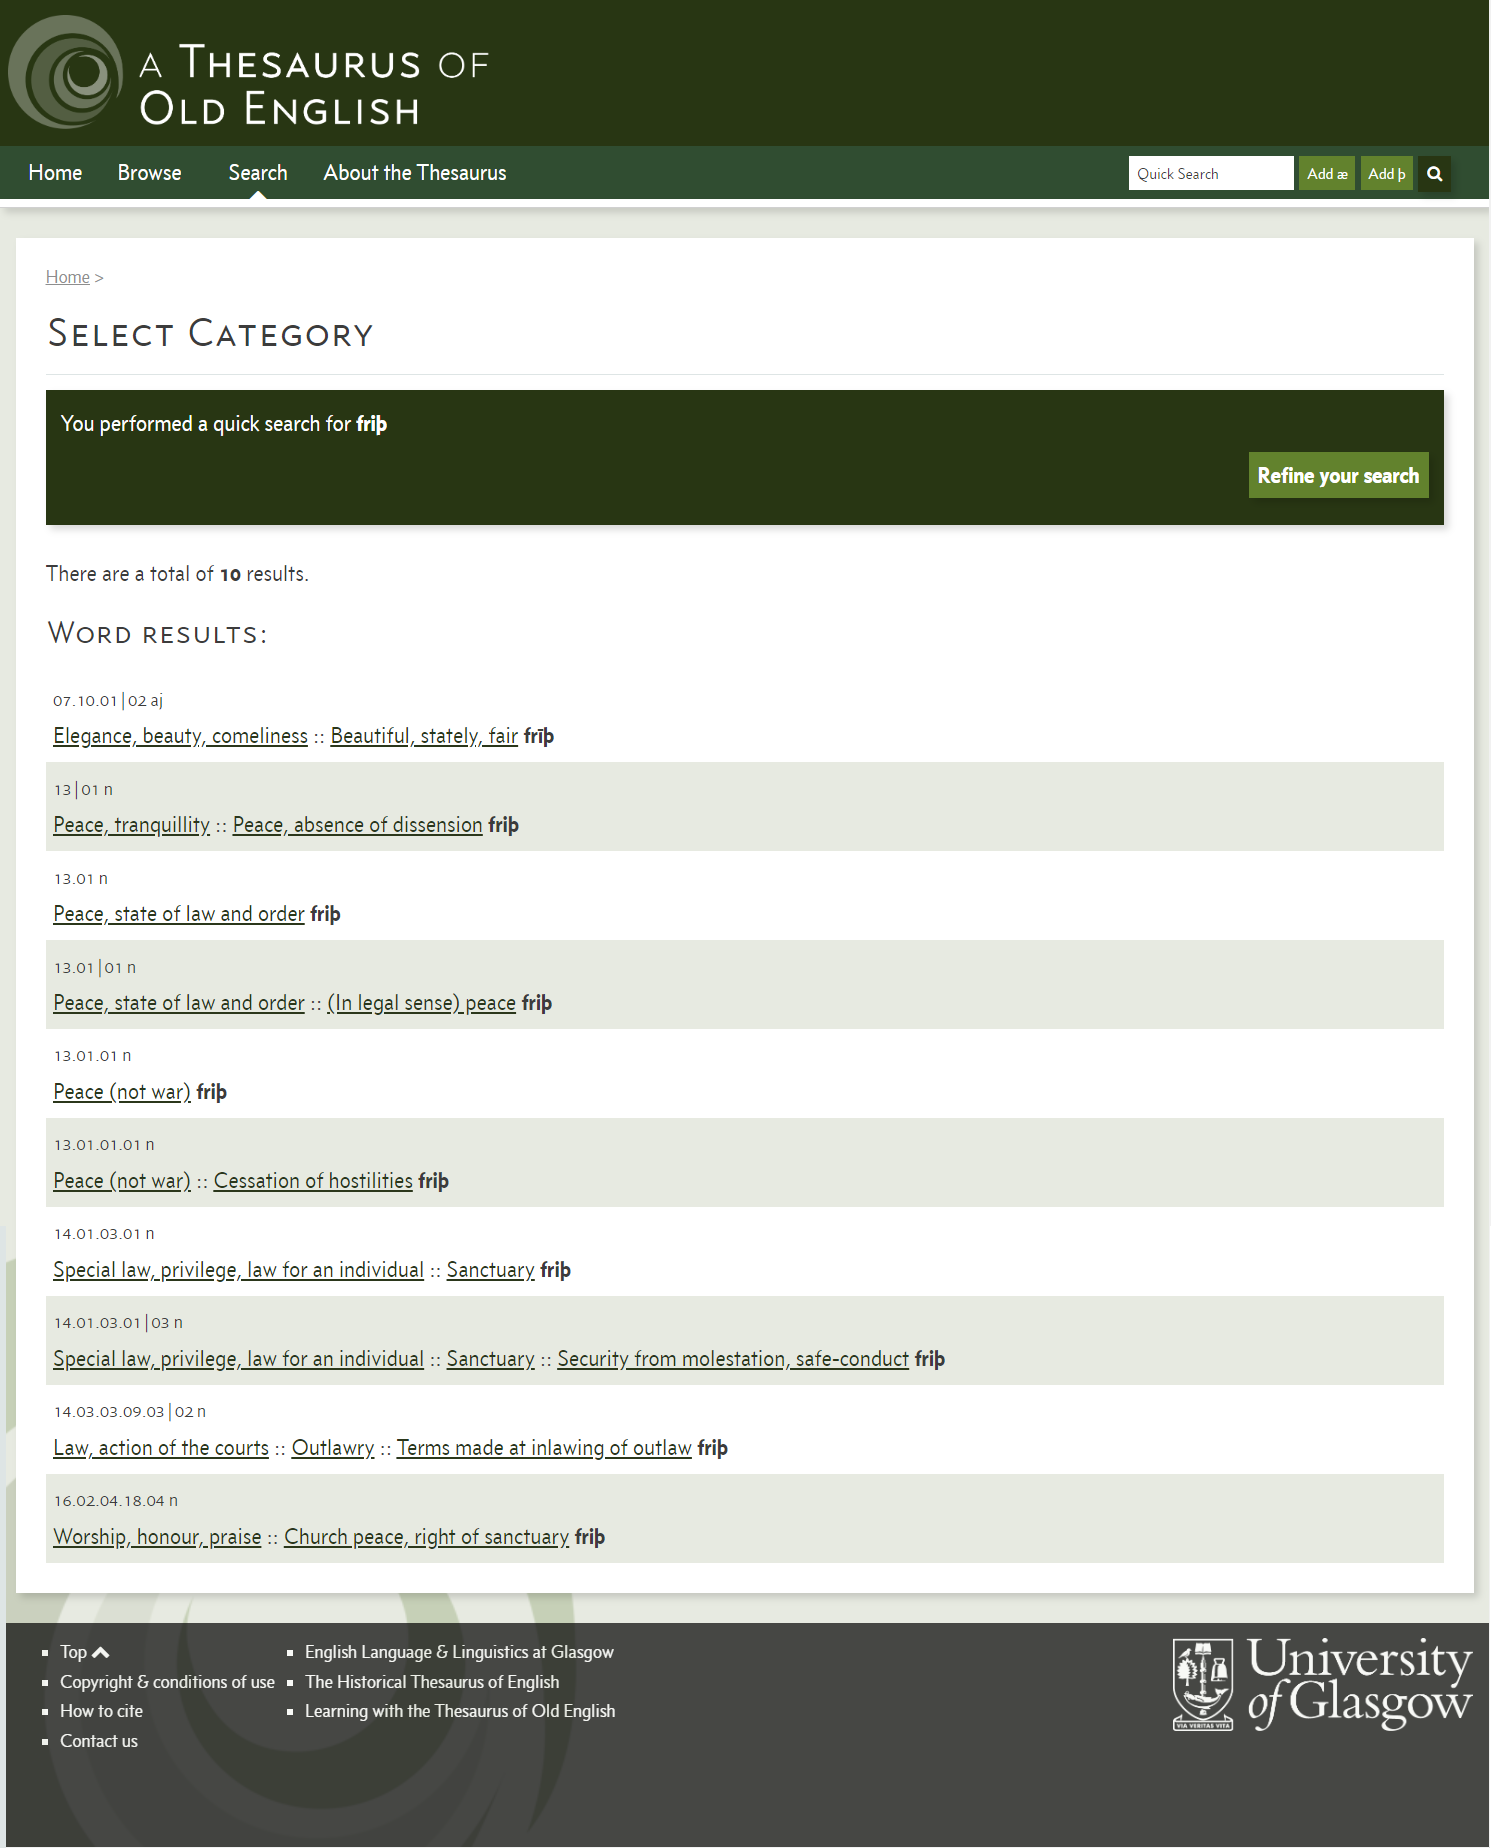
\includegraphics[width=\linewidth]{Stolk_thes-content/fig/thes/TOE4-index-frith.png}
  \caption{\textit{TOE4} index, `friþ'.}
  \label{fig:1.A:TOE4:index}
\end{figure}


%% LSM

\begin{figure}[htbp]
  \centering
    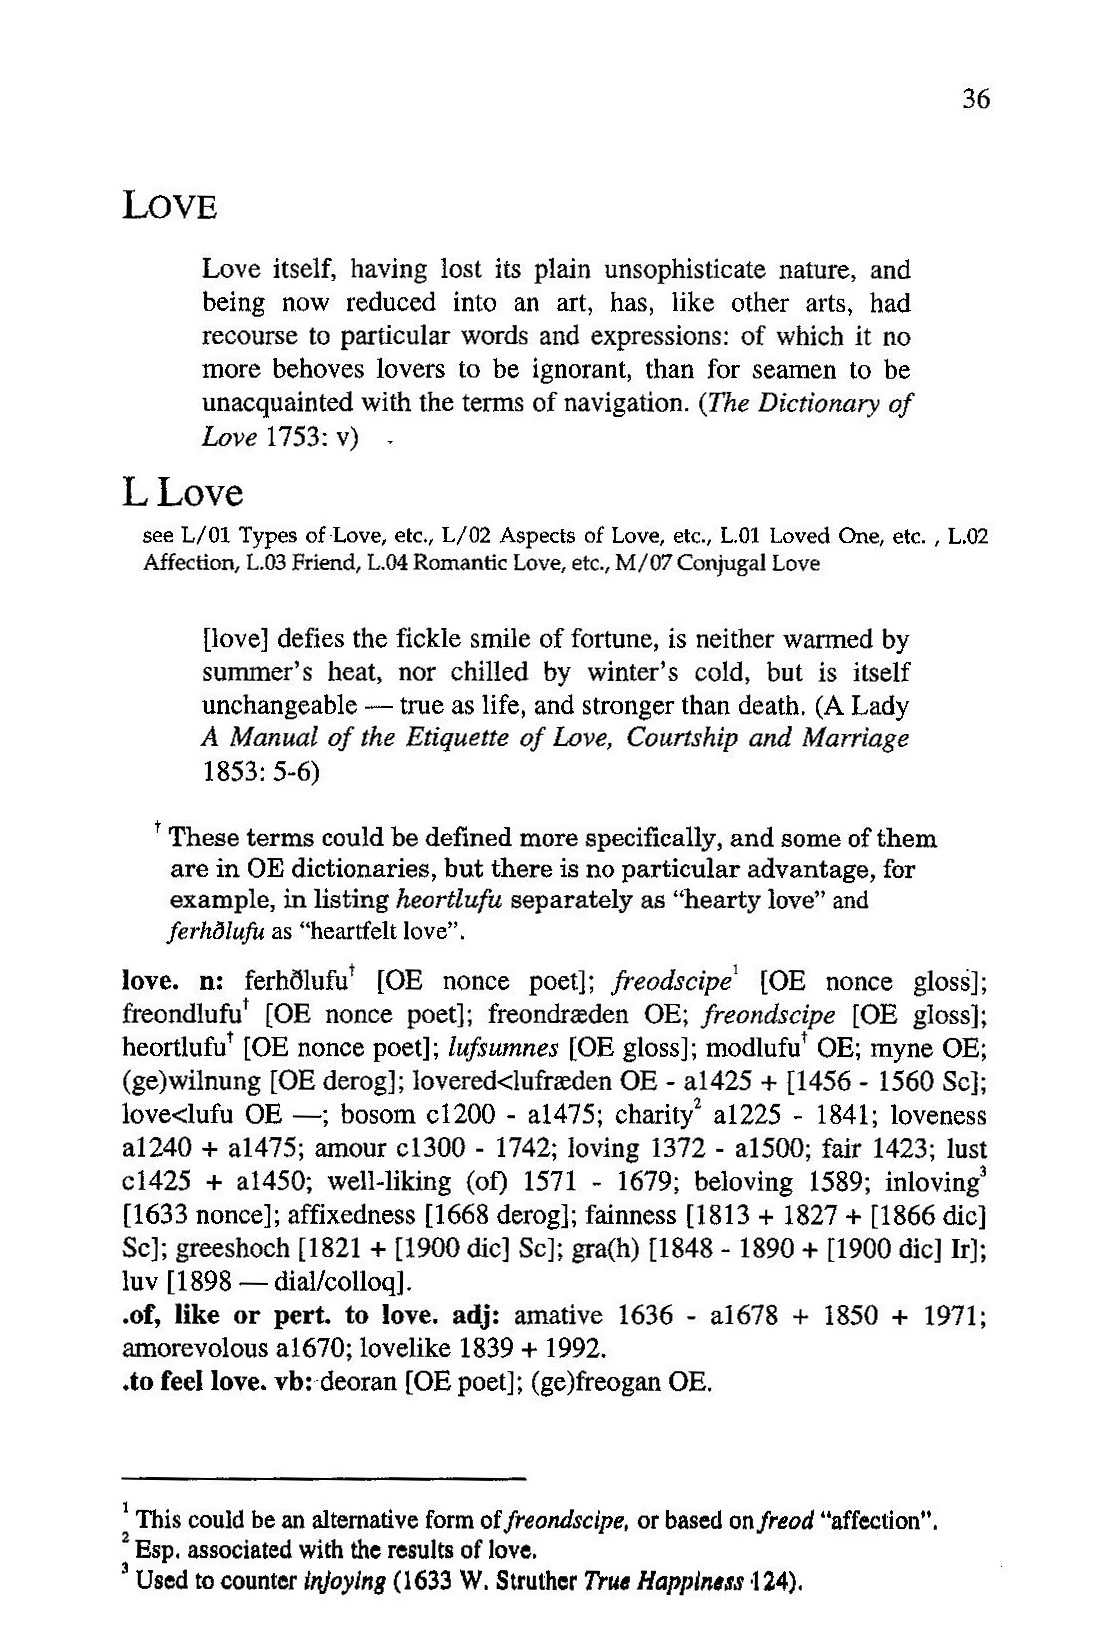
\includegraphics[width=\linewidth]{Stolk_thes-content/fig/thes/LSM-p036.jpg}
  \caption{\textit{LSM} thesaurus, p. 36.}
  \label{fig:1.A:LSM:thesaurus}
\end{figure}

\begin{figure}[htbp]
  \centering
    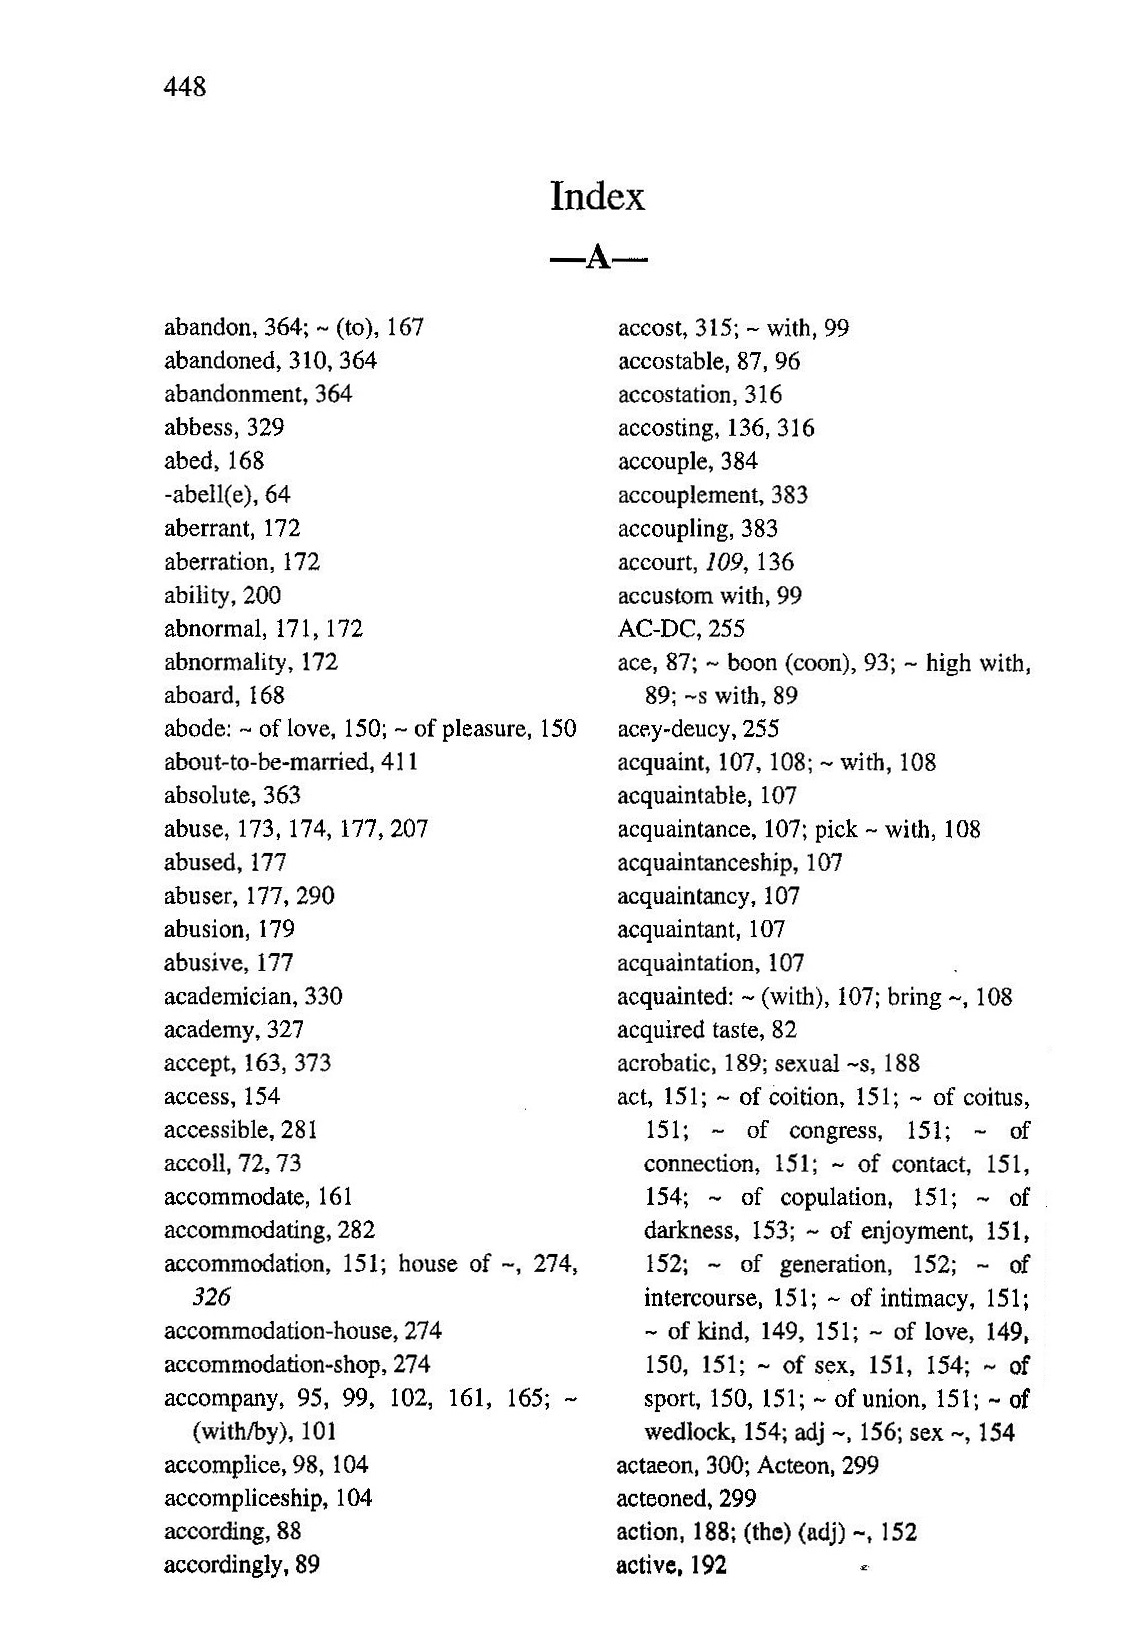
\includegraphics[width=\linewidth]{Stolk_thes-content/fig/thes/LSM-p448.jpg}
  \caption{\textit{LSM} index, p. 448.}
  \label{fig:1.A:LSM:index}
\end{figure}


%% HTE1

\begin{figure}[htbp]
  \centering
    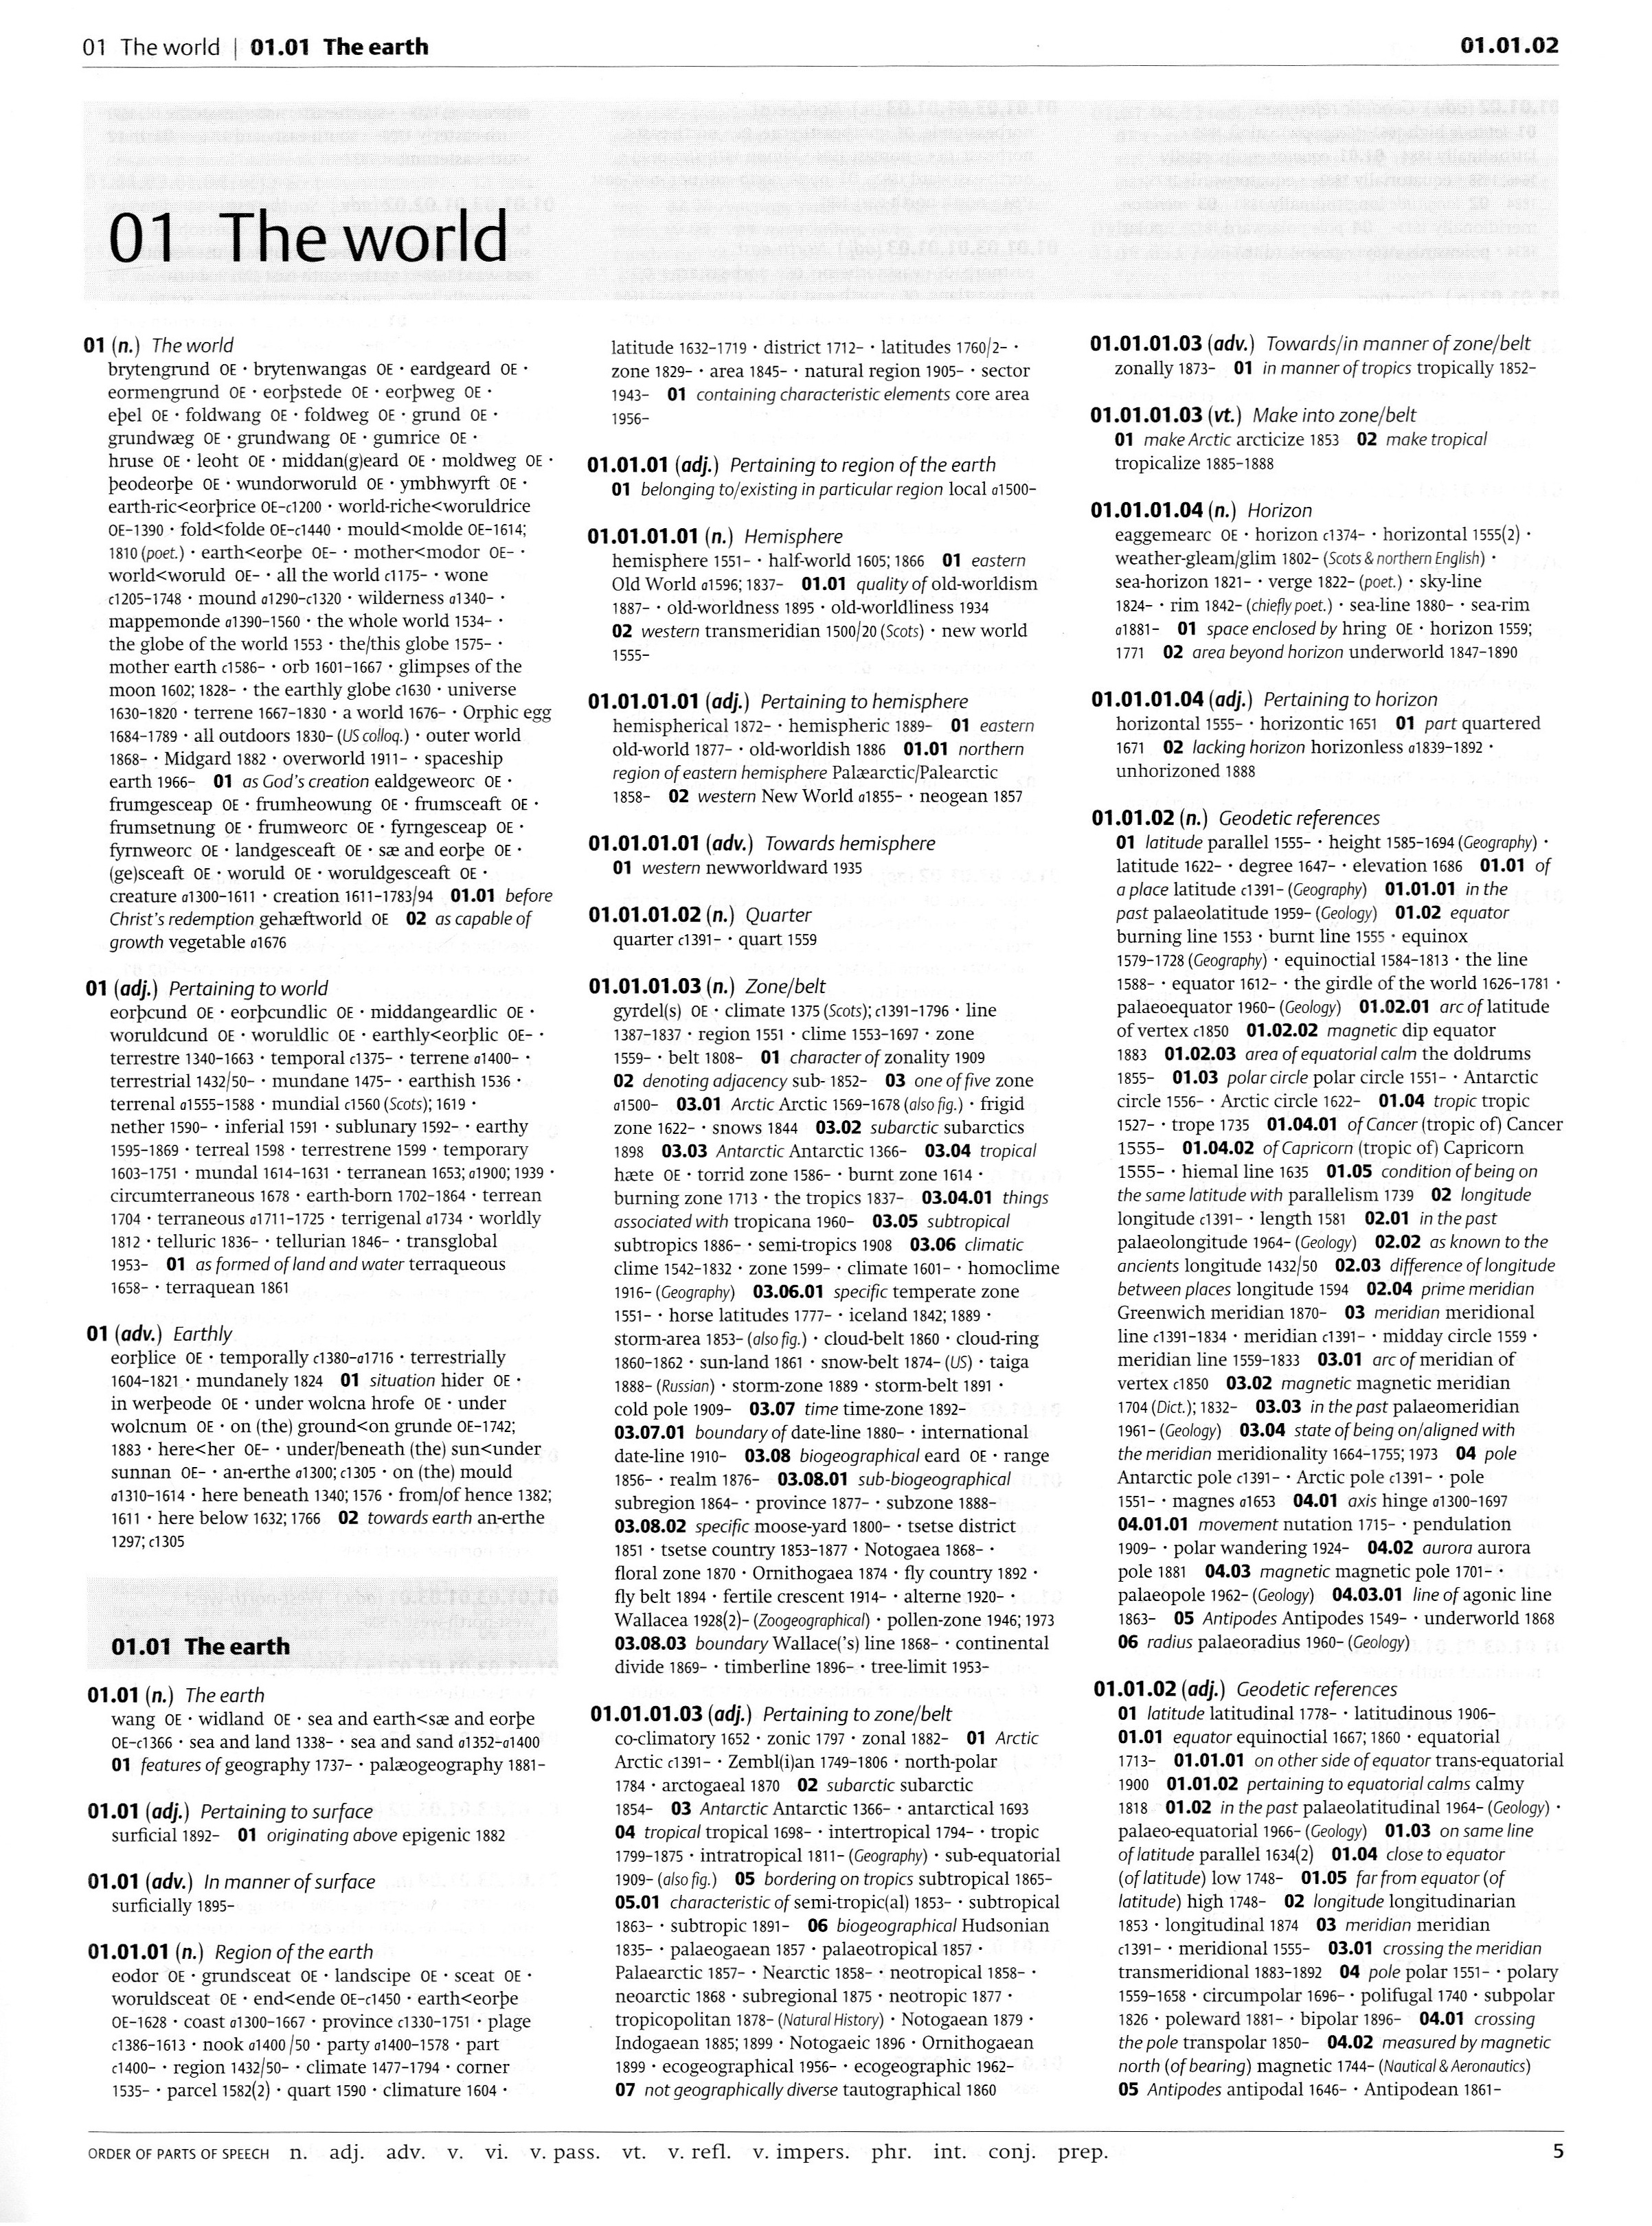
\includegraphics[width=\linewidth]{Stolk_thes-content/fig/thes/HTE1-p0005.jpg}
  \caption{\textit{HTE1} thesaurus, vol. 1, p. 5.}
  \label{fig:1.A:HTE1:thesaurus}
\end{figure}

\begin{figure}[htbp]
  \centering
    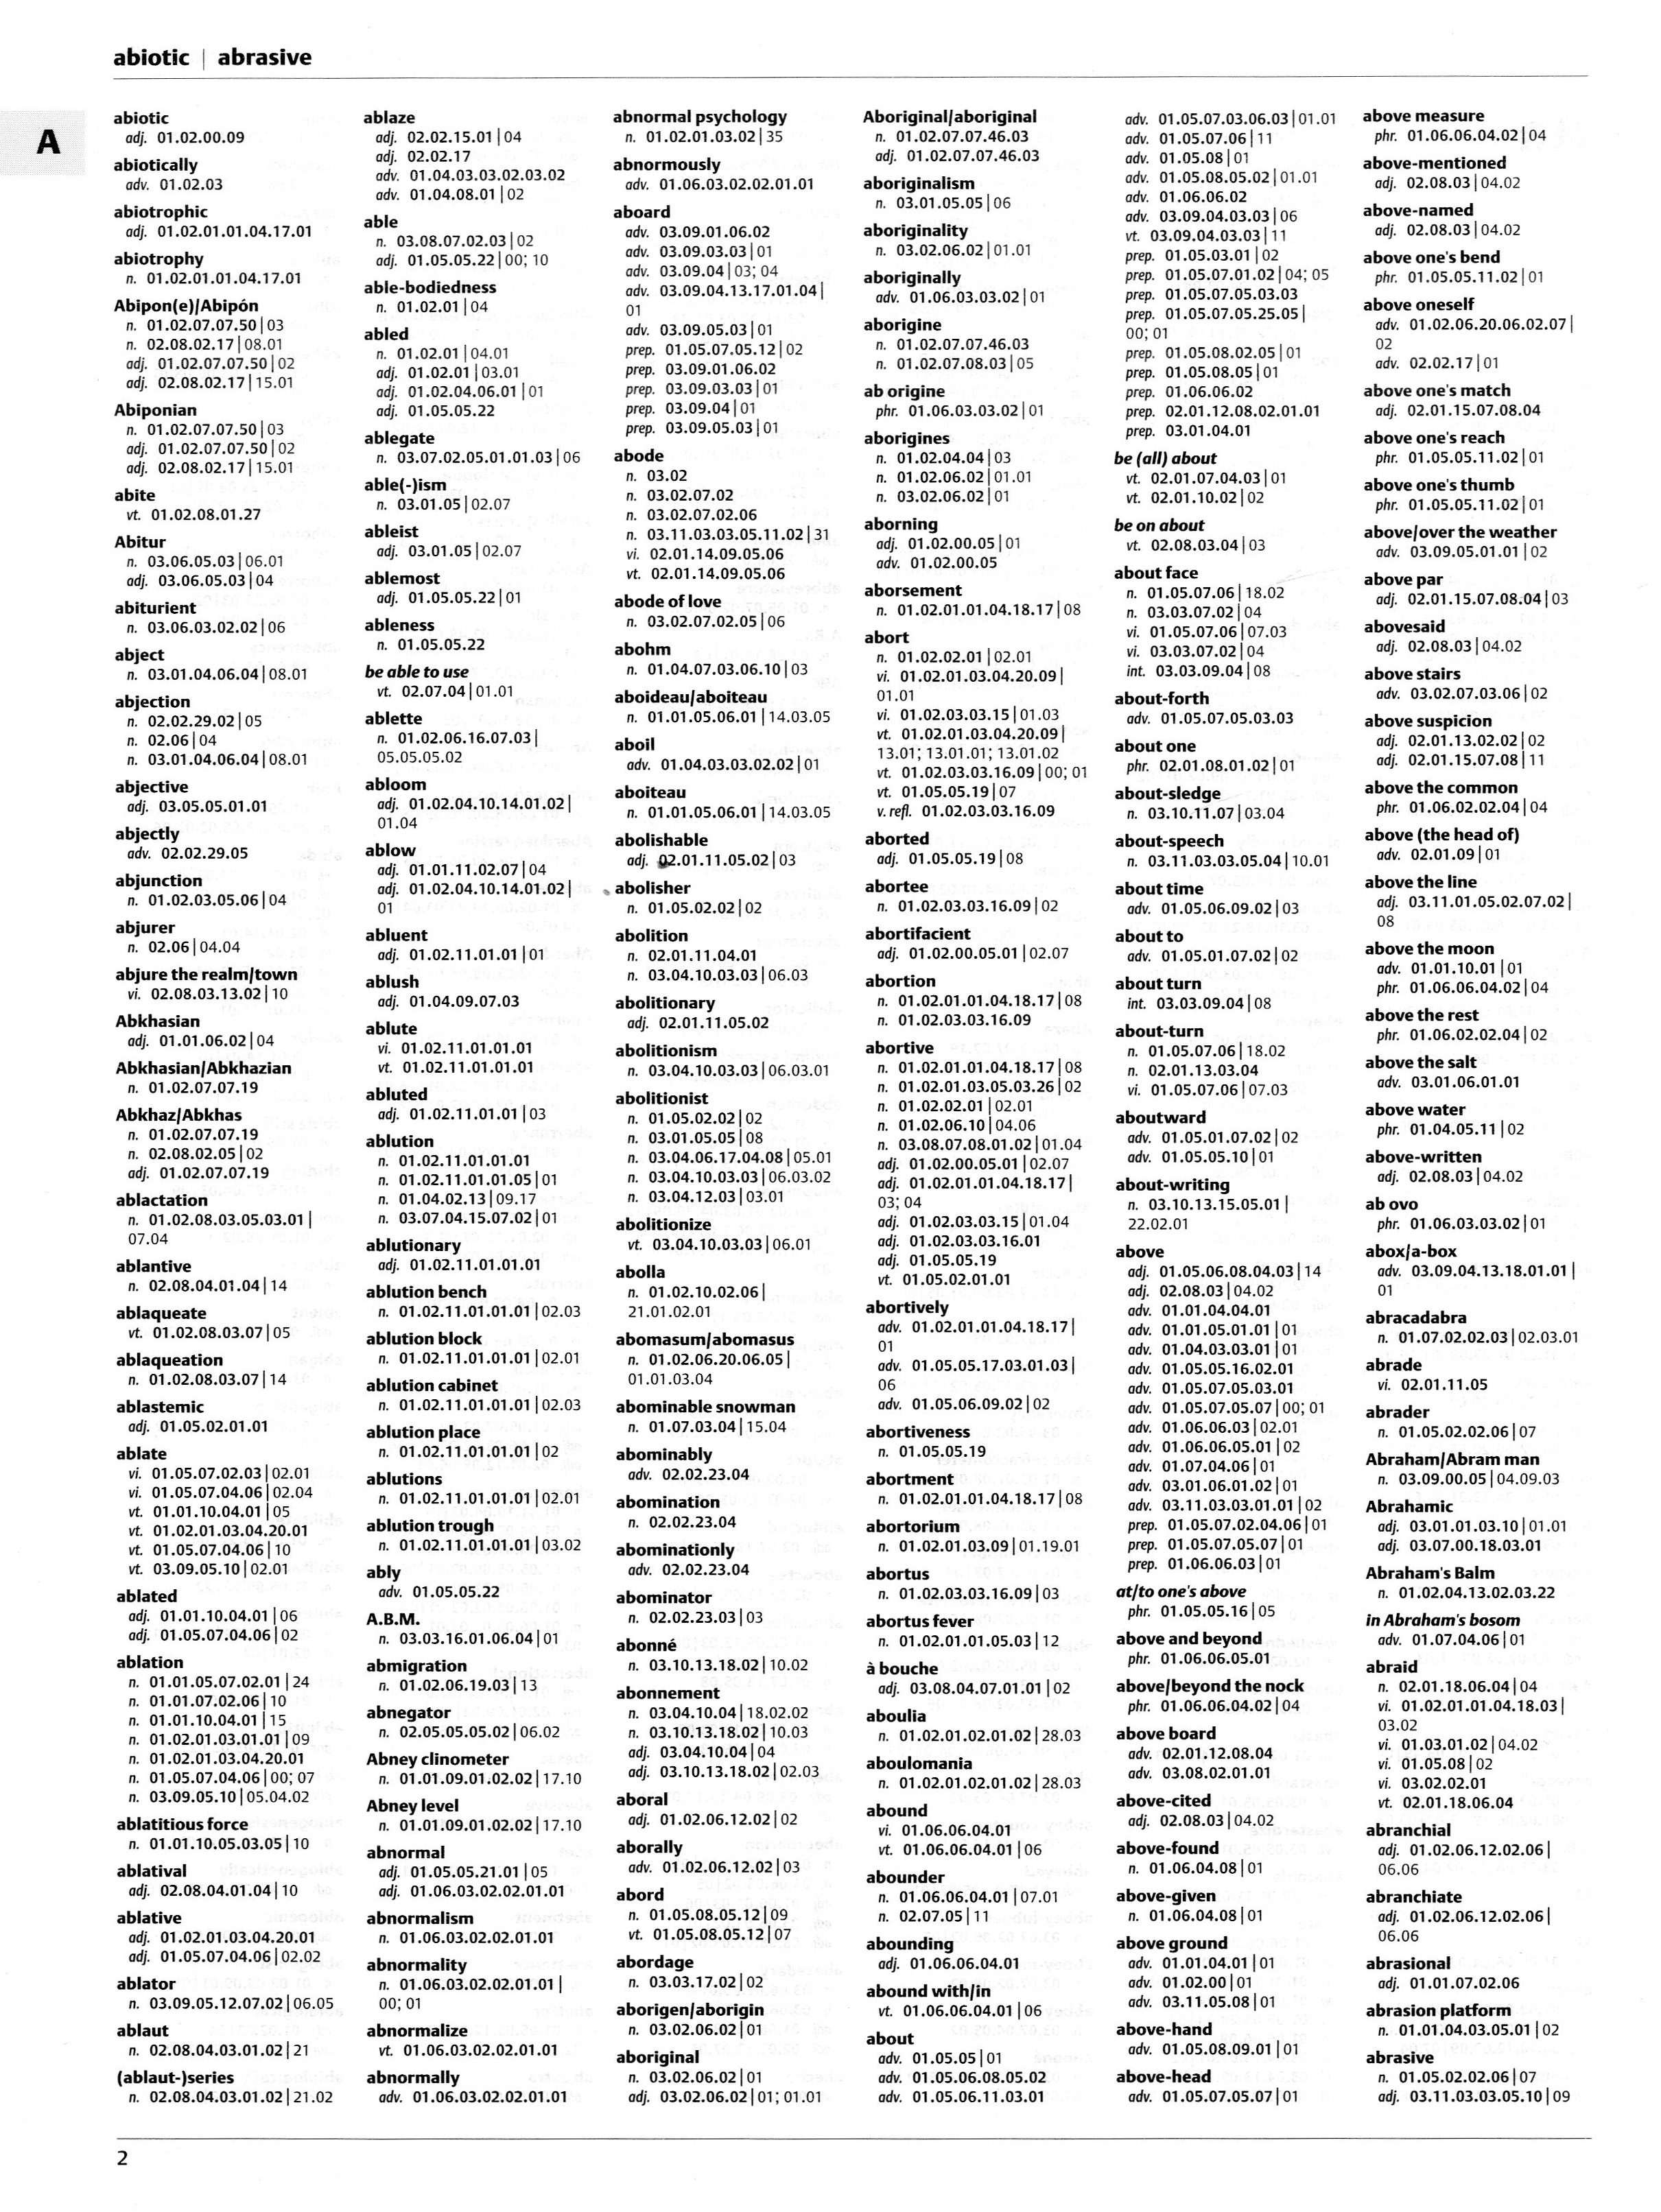
\includegraphics[width=\linewidth]{Stolk_thes-content/fig/thes/HTE1-vol2-p002.jpg}
  \caption{\textit{HTE1} index, vol. 2, p. 2.}
  \label{fig:1.A:HTE1:index}
\end{figure}


%% HTE2

\begin{figure}[htbp]
  \centering
    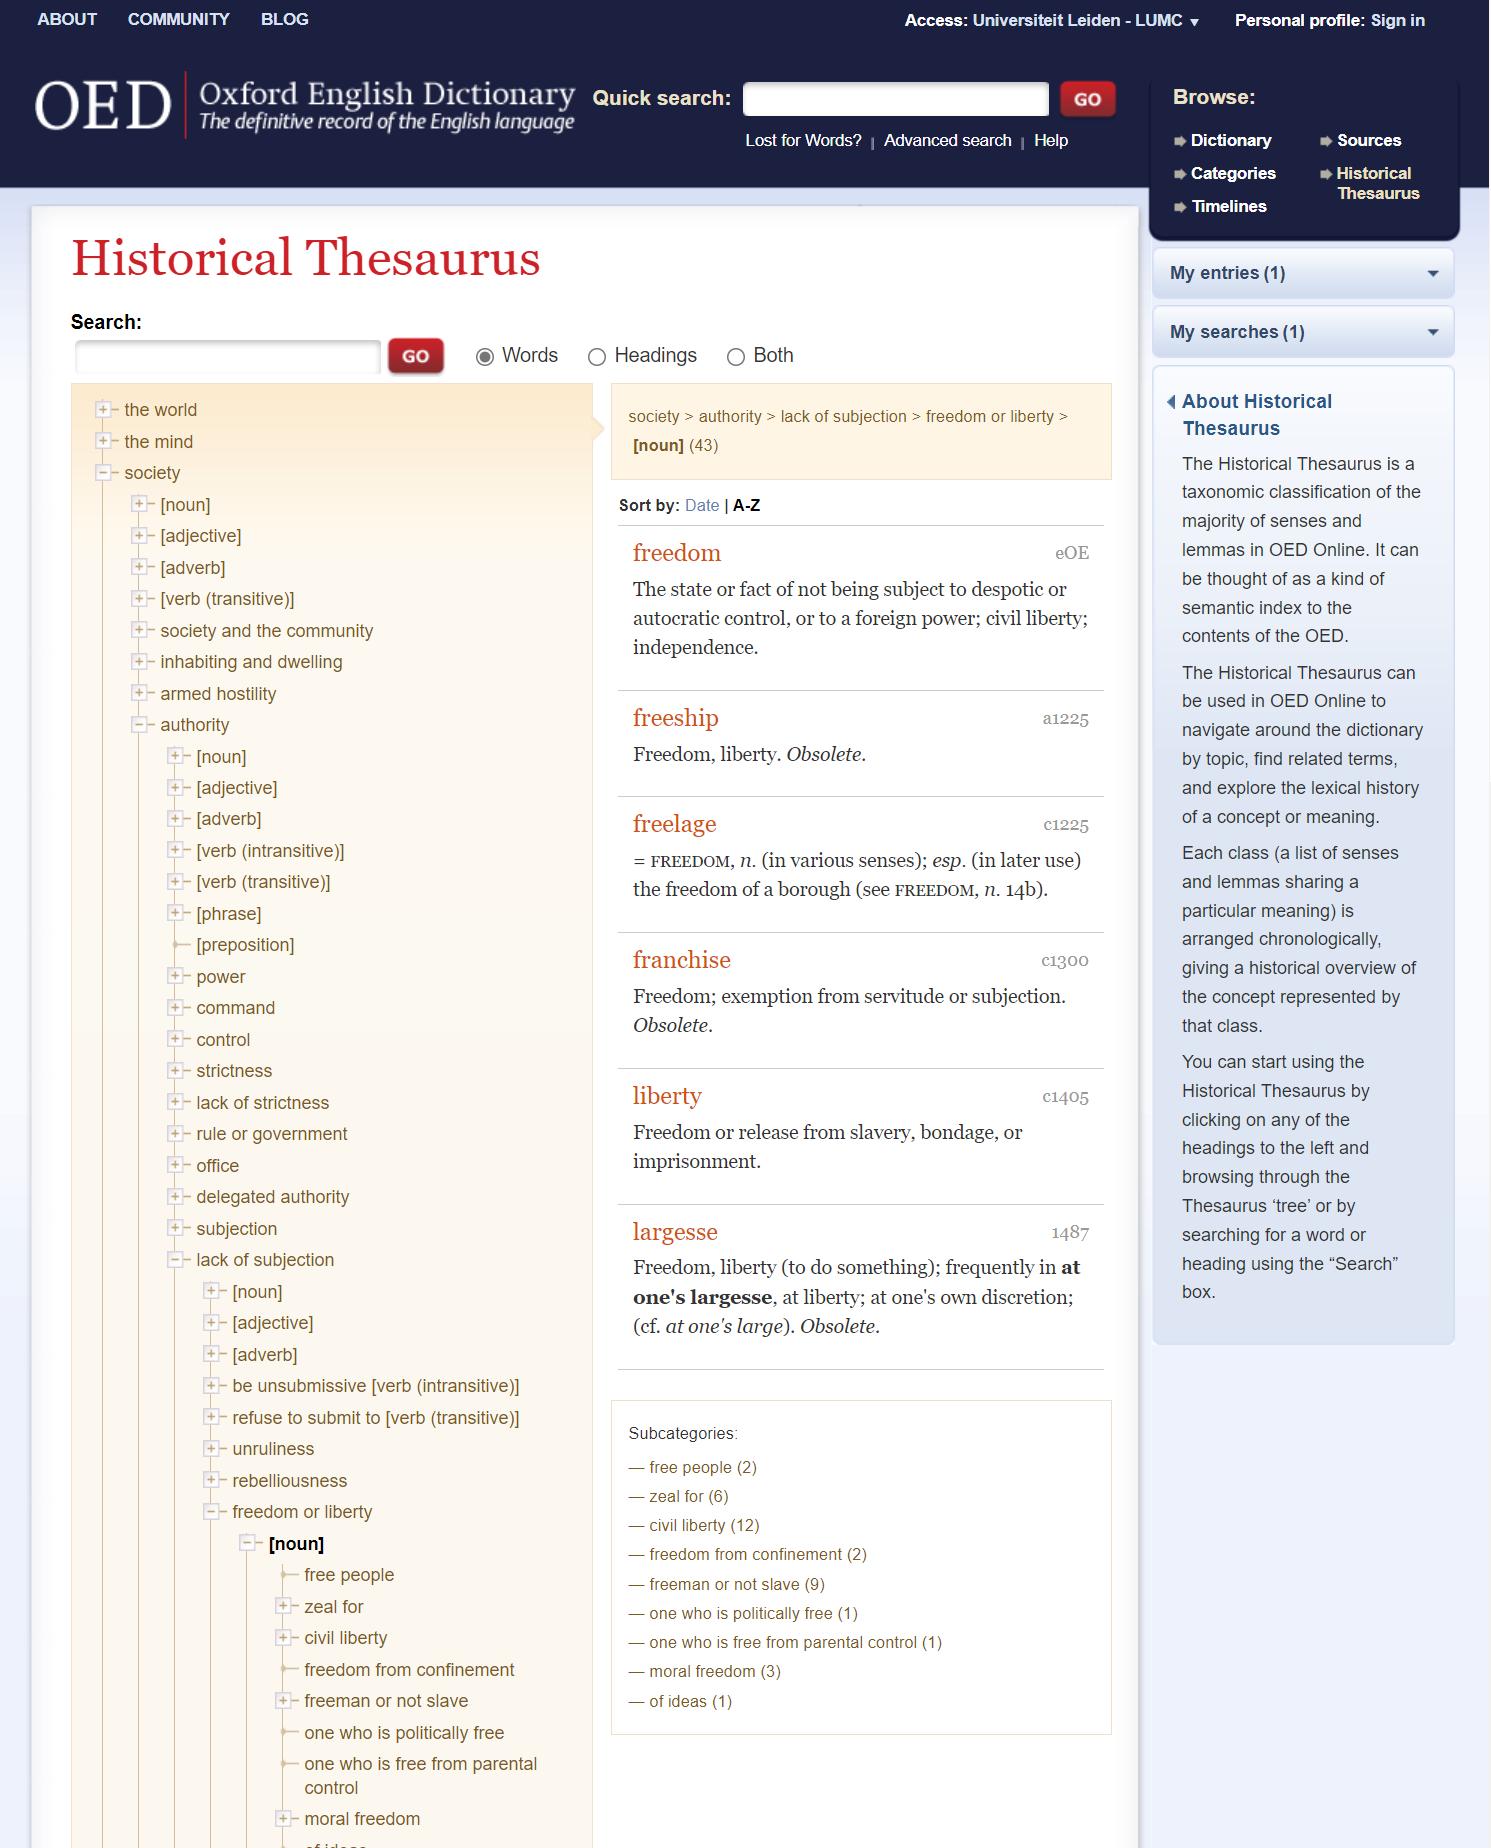
\includegraphics[width=\linewidth]{Stolk_thes-content/fig/thes/HTE2-thesaurus-freedomliberty.png}
  \caption{\textit{HTE2} thesaurus, category ``freedom or liberty''.}
  \label{fig:1.A:HTE2:thesaurus}
\end{figure}

\begin{figure}[htbp]
  \centering
    \includegraphics[width=\linewidth]{Stolk_thes-content/fig/thes/HTE2-ìndex-freedom.png}
  \caption{\textit{HTE2} index, `freedom'.}
  \label{fig:1.A:HTE2:index}
\end{figure}


%% HTE3

\begin{figure}[htbp]
  \centering
    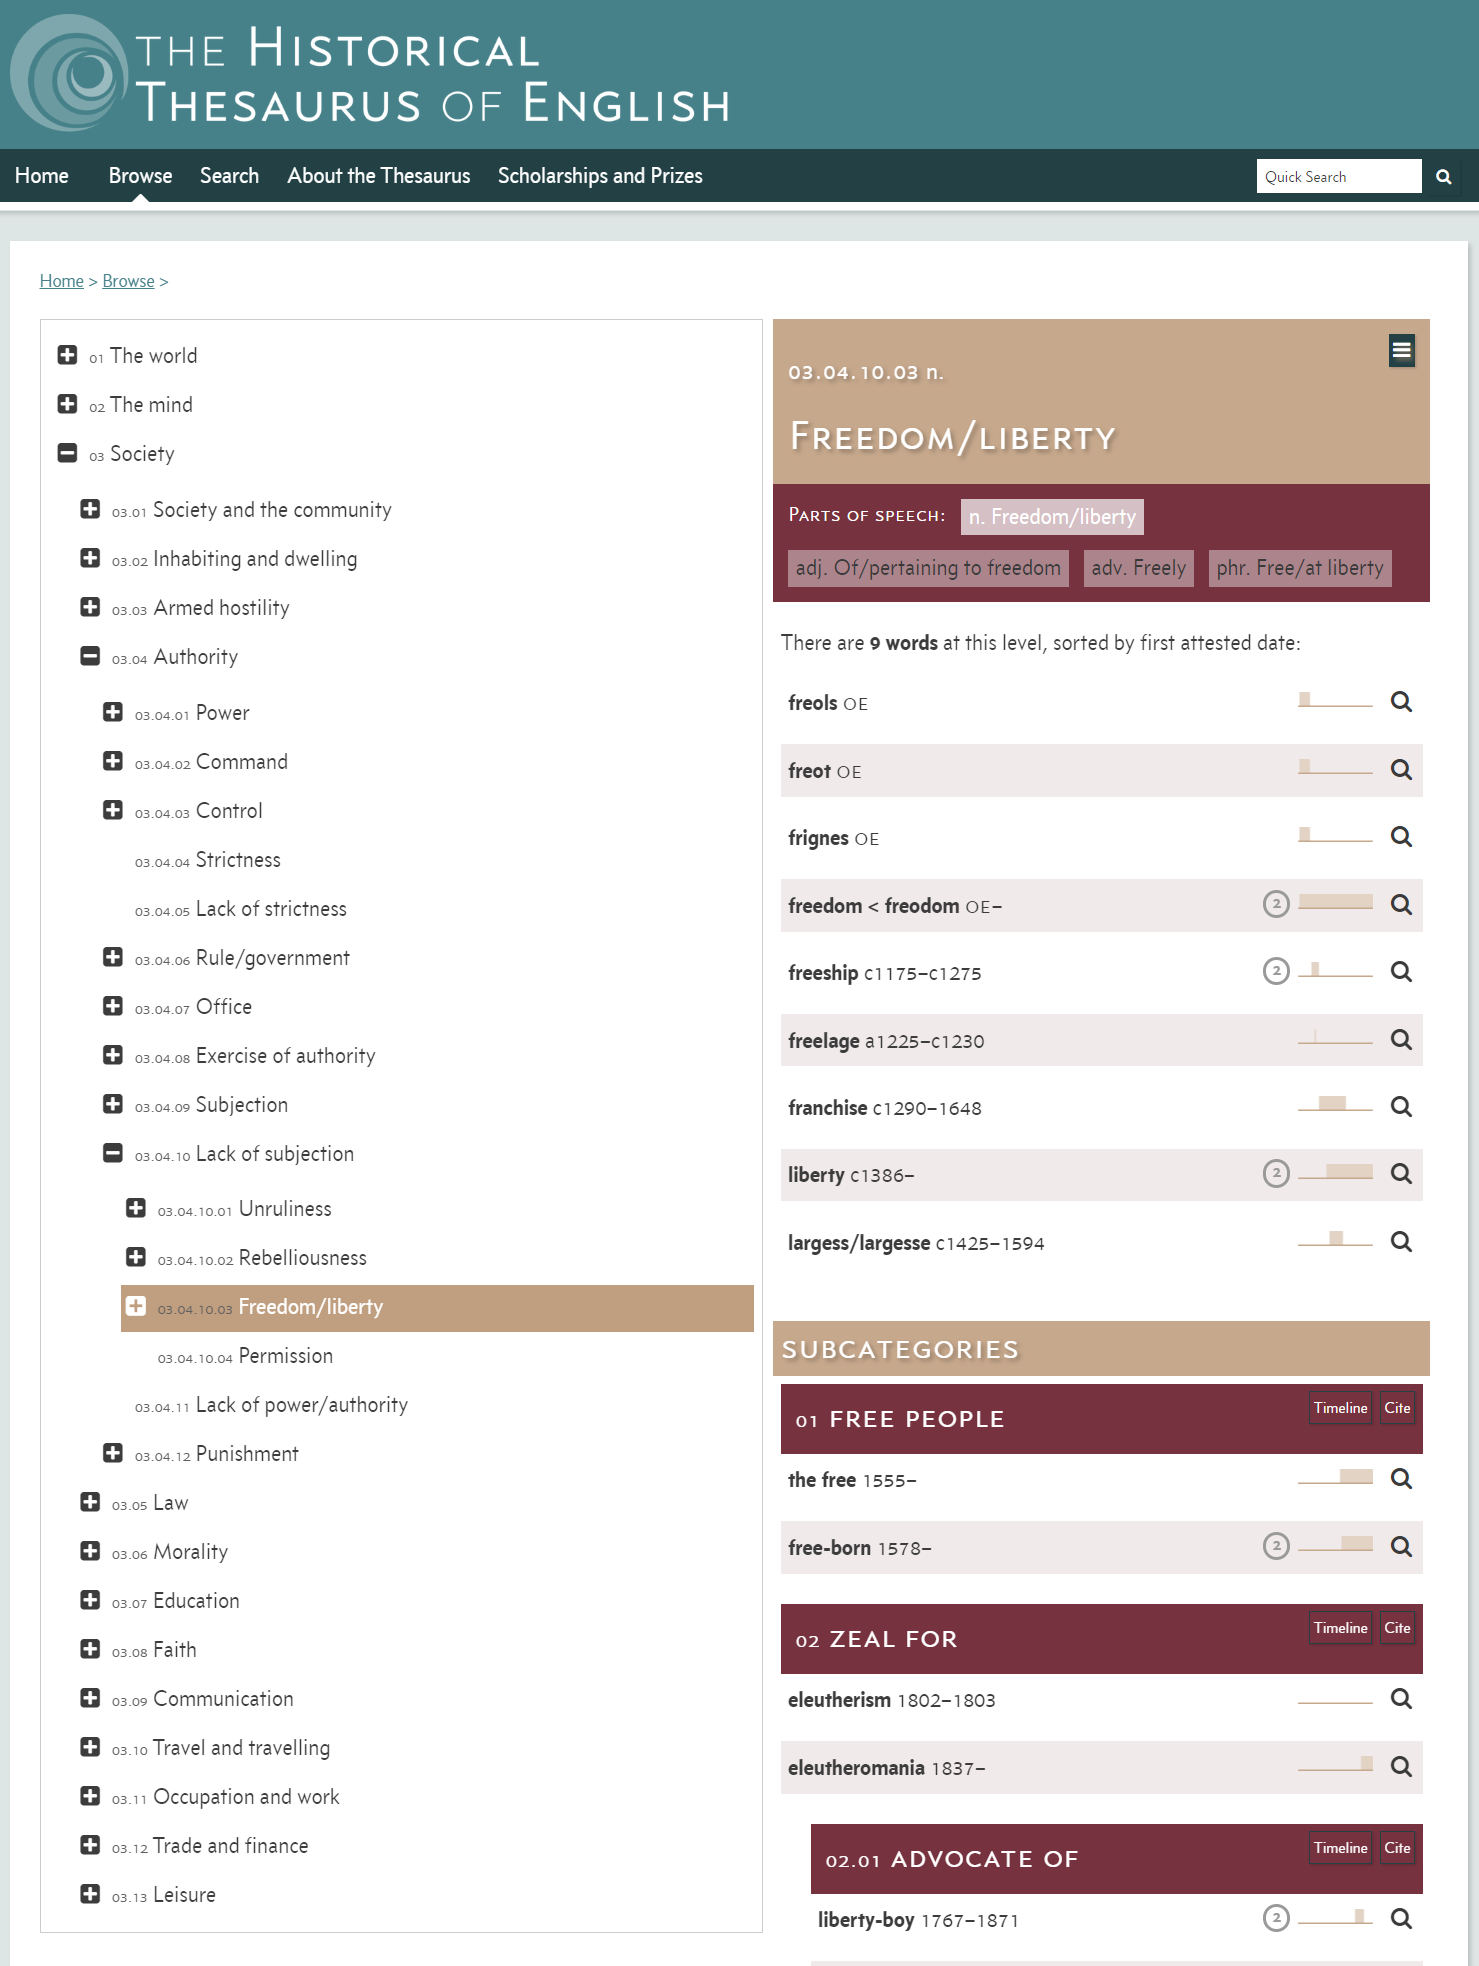
\includegraphics[width=\linewidth]{Stolk_thes-content/fig/thes/HTE3-thesaurus-freedomliberty.png}
  \caption{\textit{HTE3} thesaurus, category ``03.04.10.03 n. Freedom/liberty''.}
  \label{fig:1.A:HTE3:thesaurus}
\end{figure}

\begin{figure}[htbp]
  \centering
    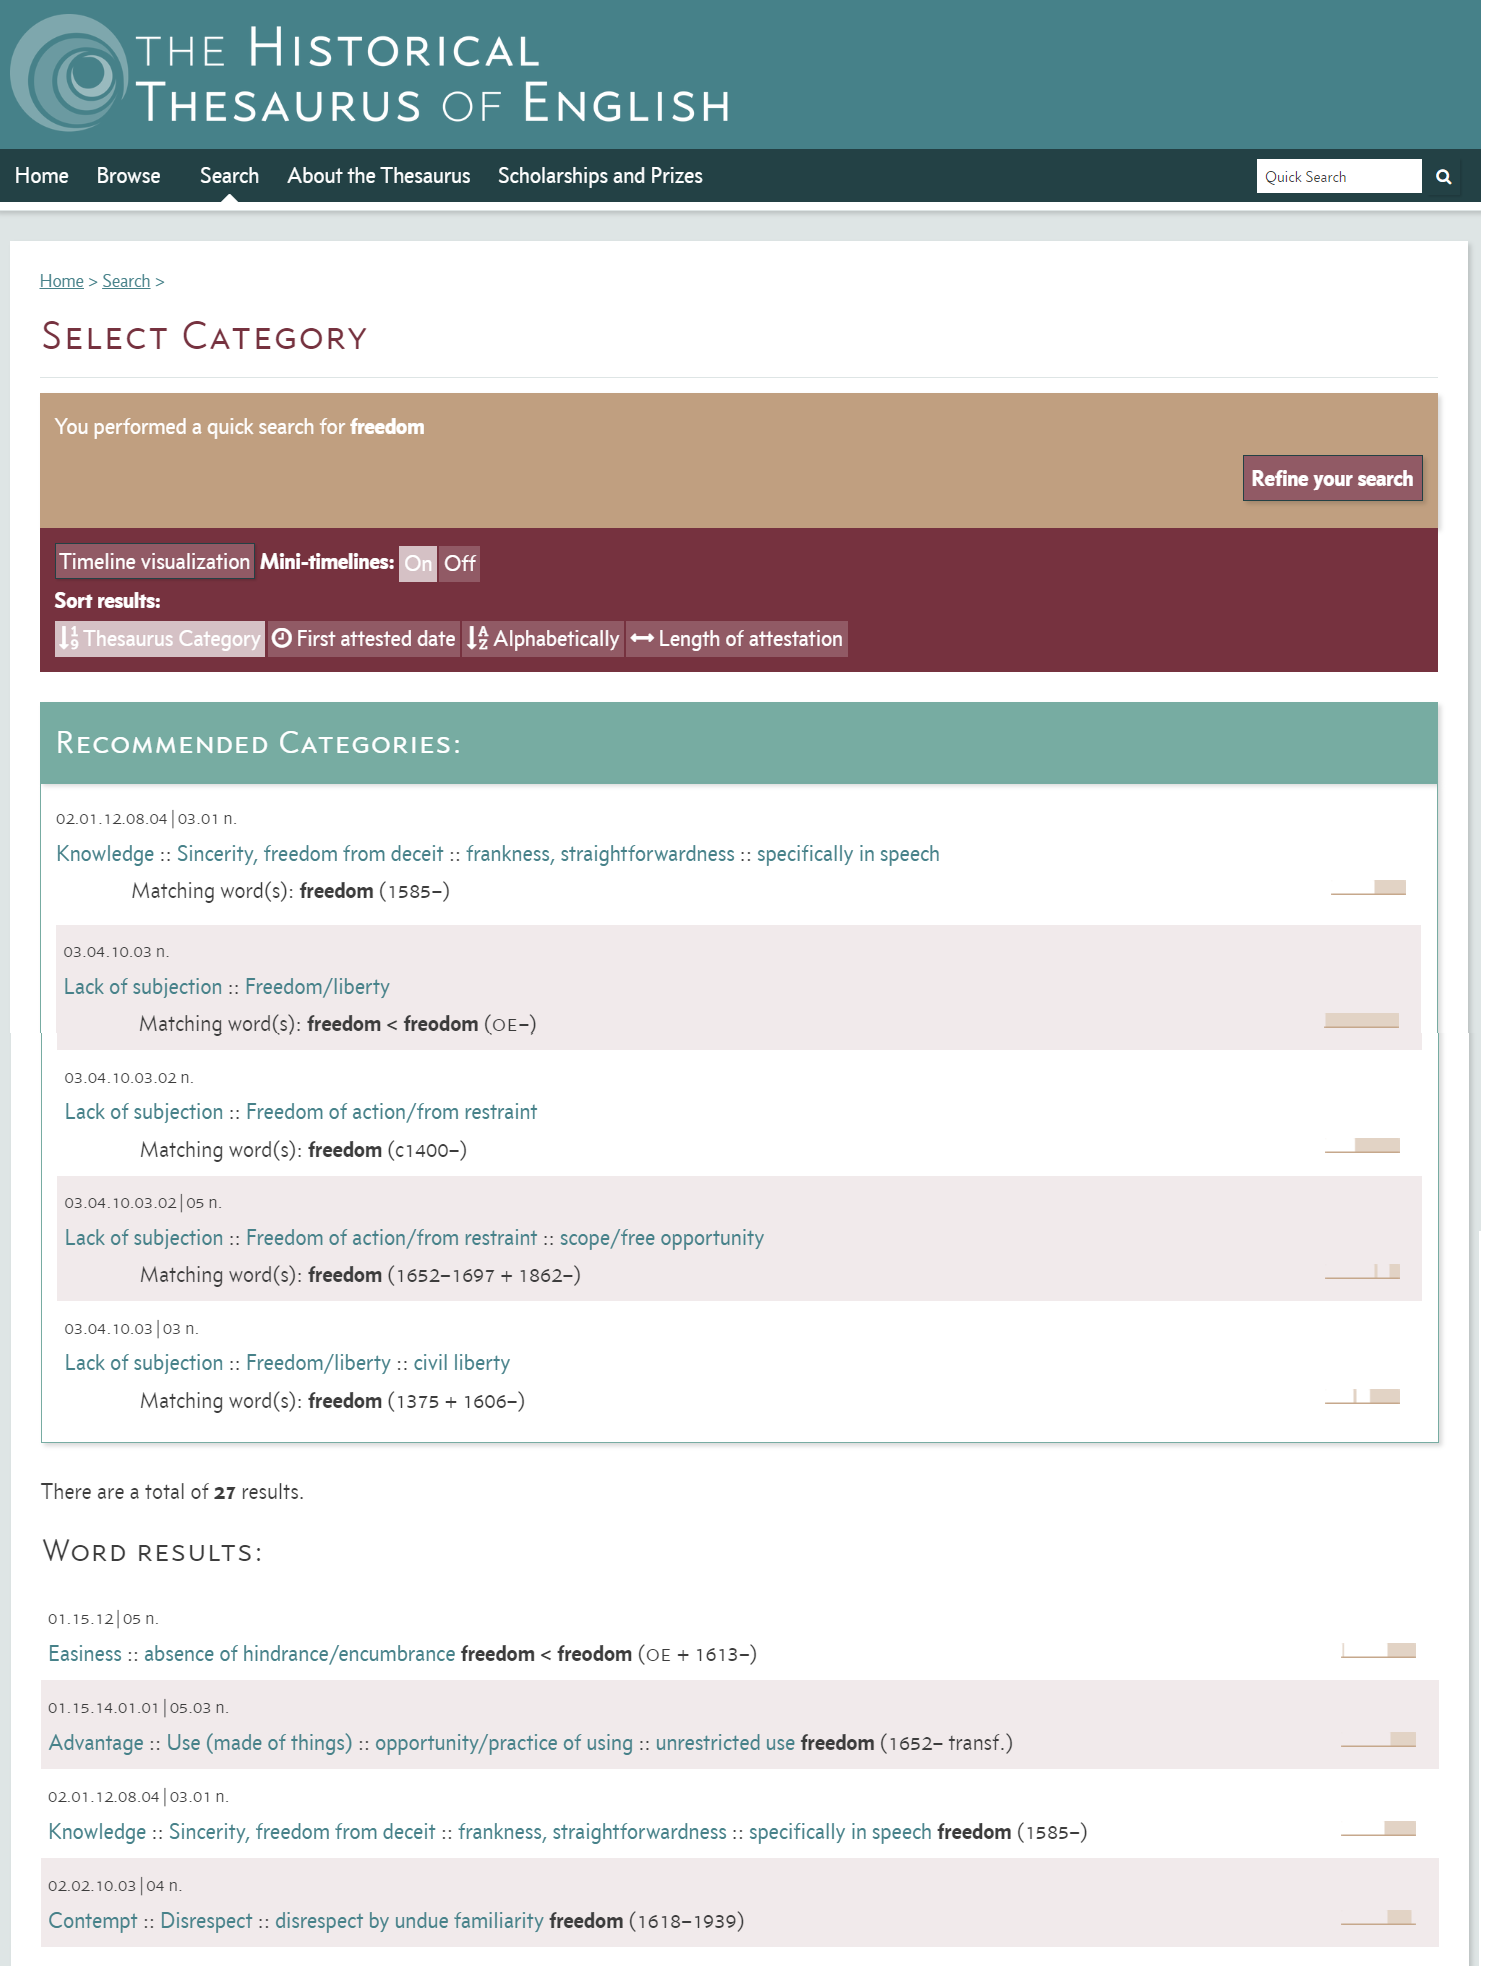
\includegraphics[width=\linewidth]{Stolk_thes-content/fig/thes/HTE3-index-freedom.png}
  \caption{\textit{HTE3} index, `freedom'.}
  \label{fig:1.A:HTE3:index}
\end{figure}


%% HTS

\begin{figure}[htbp]
  \centering
    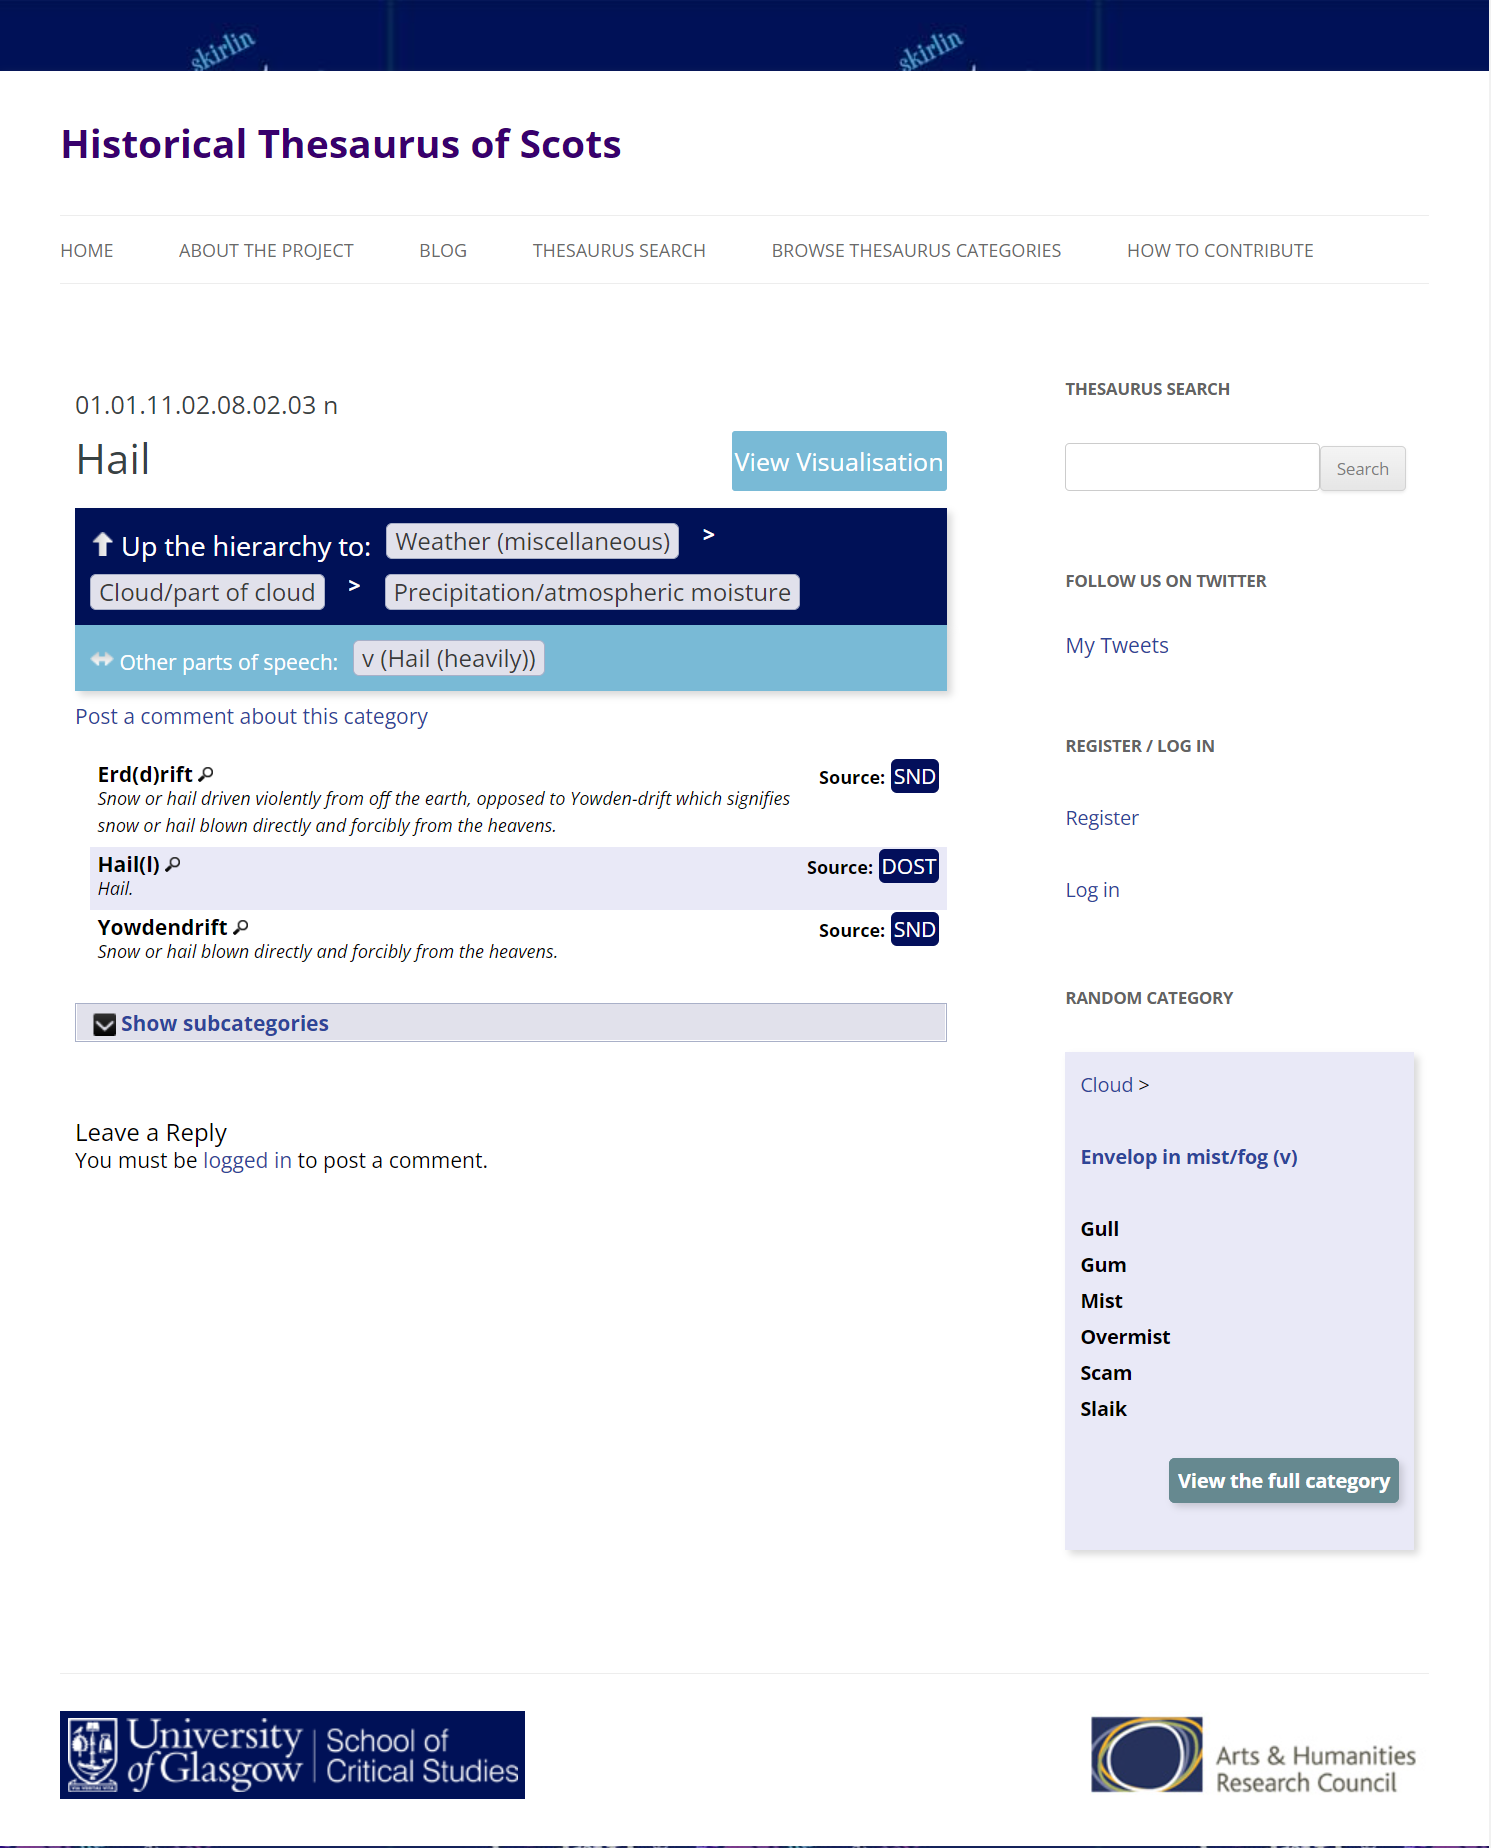
\includegraphics[width=\linewidth]{Stolk_thes-content/fig/thes/HTS-thesaurus-hail.png}
  \caption{\textit{HTS} thesaurus, category ``01.01.11.02.08.02.03 n. Hail''.}
  \label{fig:1.A:HTS:thesaurus}
\end{figure}

\begin{figure}[htbp]
  \centering
    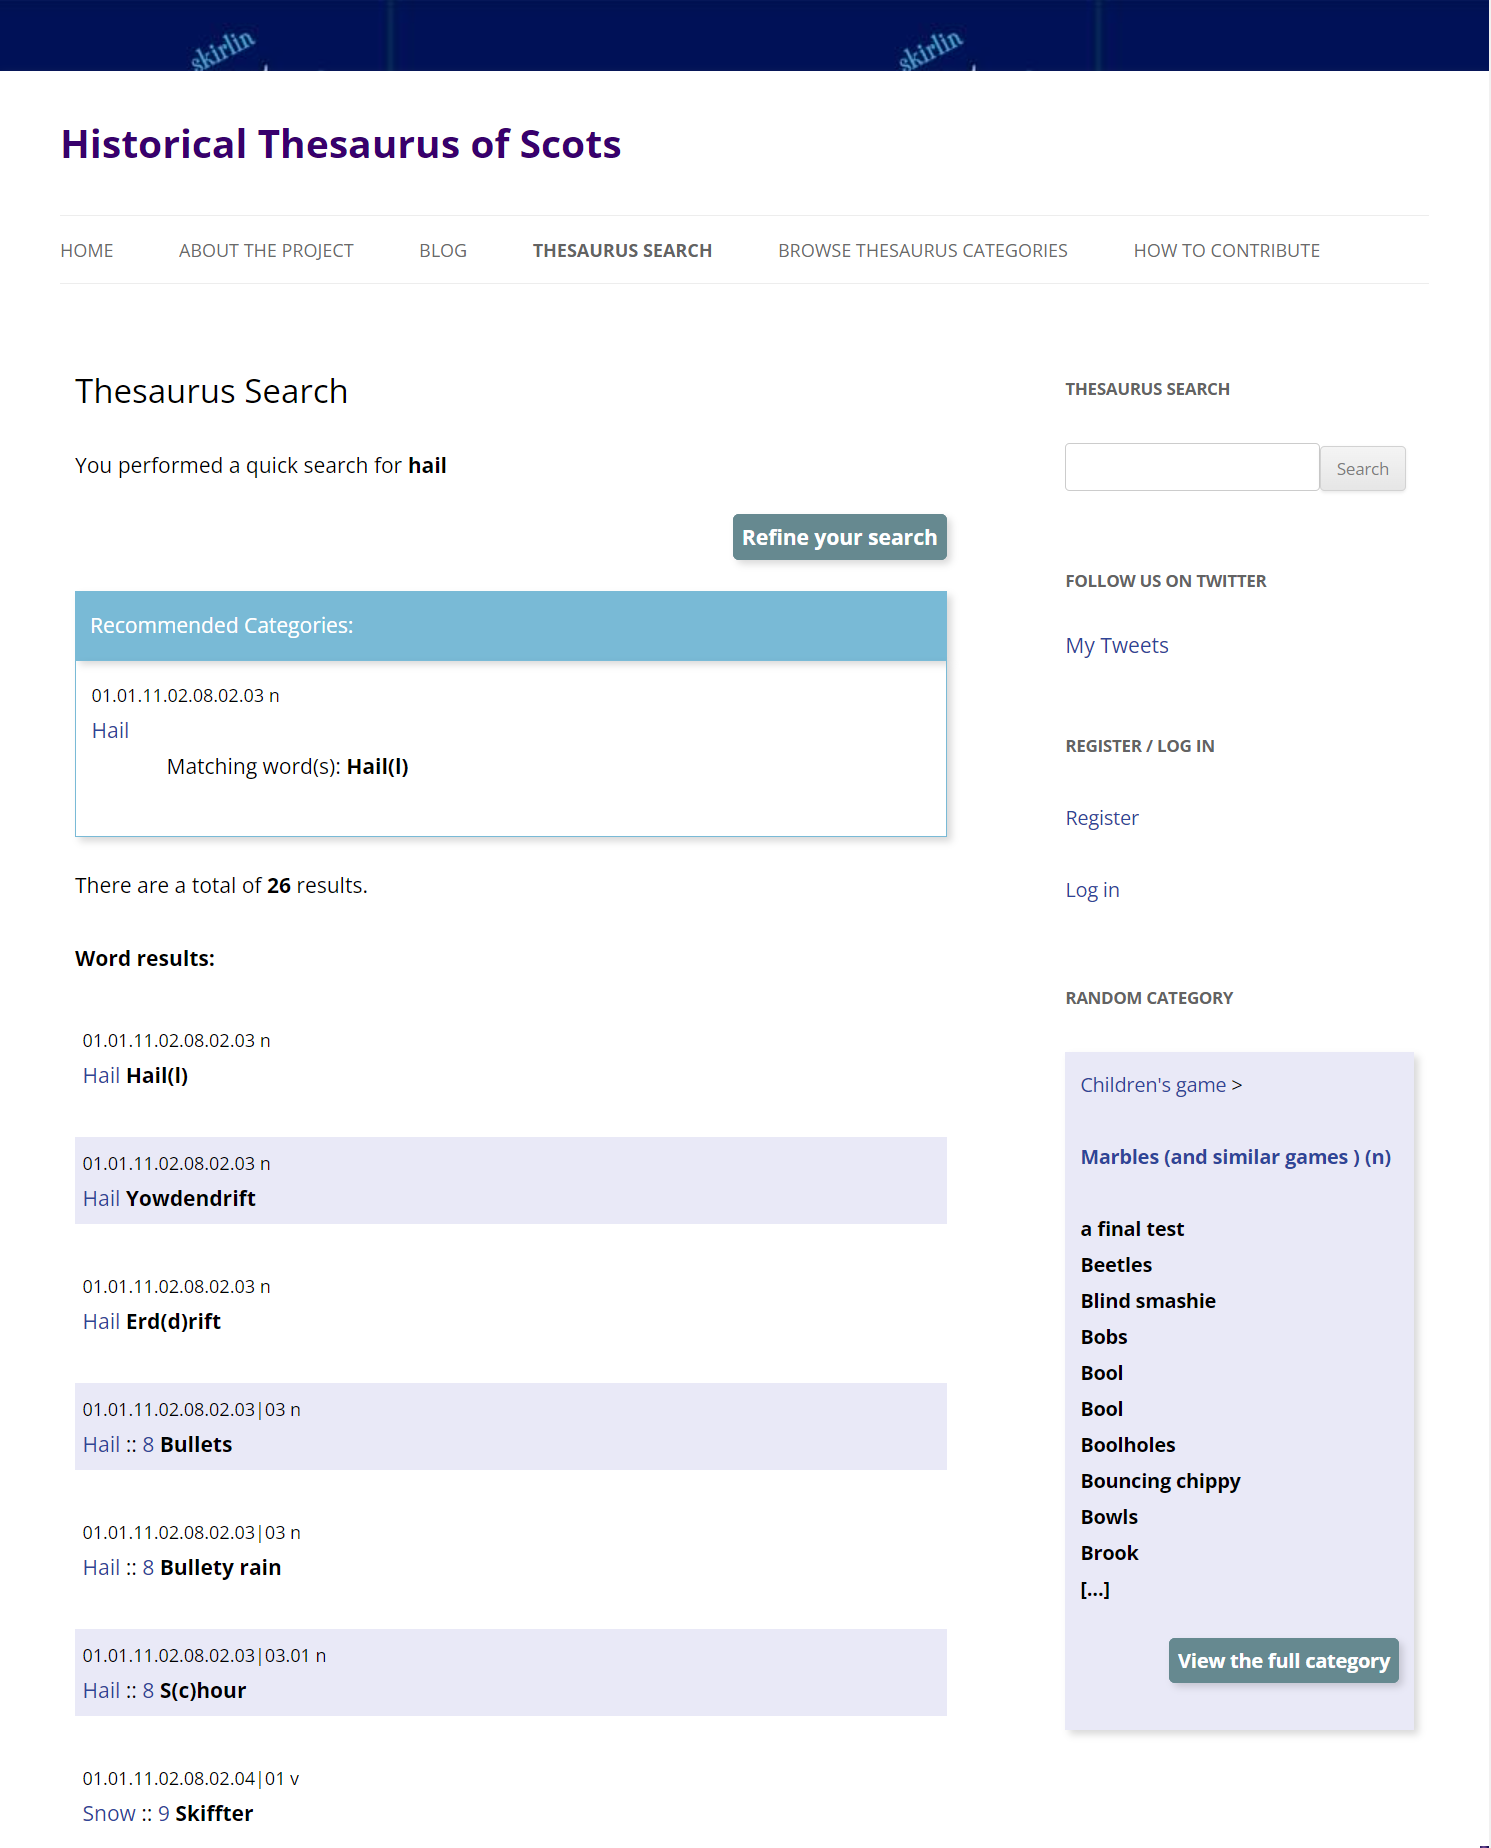
\includegraphics[width=\linewidth]{Stolk_thes-content/fig/thes/HTS-index-hail.png}
  \caption{\textit{HTS} index, `hail'.}
  \label{fig:1.A:HTS:index}
\end{figure}


%% BTH

\begin{figure}[htbp]
  \centering
    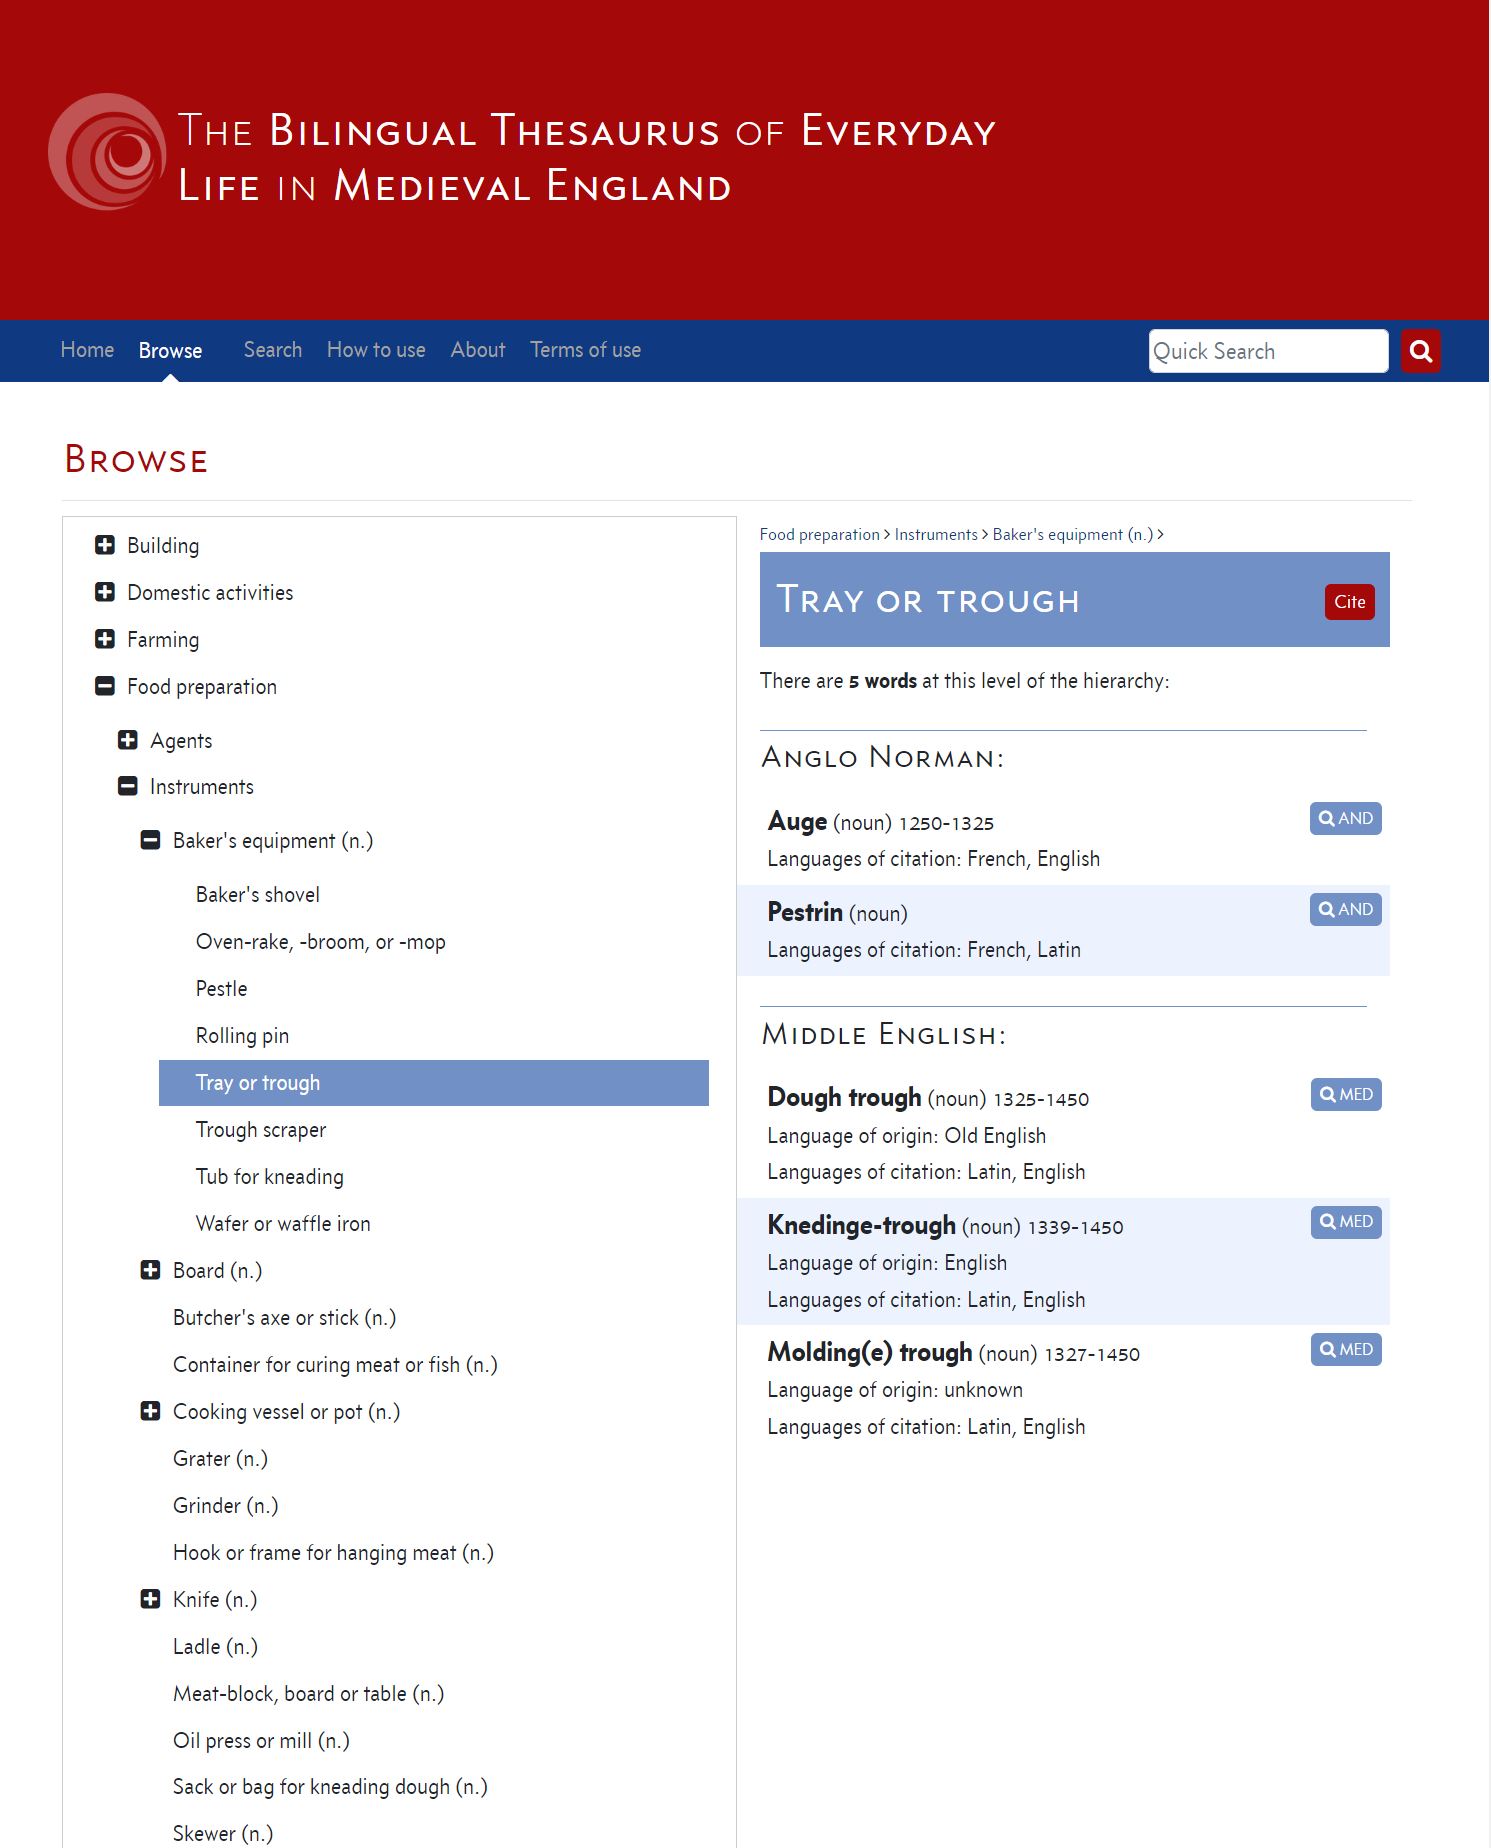
\includegraphics[width=\linewidth]{Stolk_thes-content/fig/thes/BTH-thesaurus-traytrough.png}
  \caption{\textit{BTH} thesaurus, category ``Tray or trough''.}
  \label{fig:1.A:BTH:thesaurus}
\end{figure}

\begin{figure}[htbp]
  \centering
    \includegraphics[width=\linewidth]{Stolk_thes-content/fig/thes/BTH-ìndex-auge.png}
  \caption{\textit{BTH} index, `auge'.}
  \label{fig:1.A:BTH:index}
\end{figure}






\begin{comment}
\noindent
\begin{figure}[h]
  \centering
  \begin{minipage}{.5\textwidth}
    \raggedright
    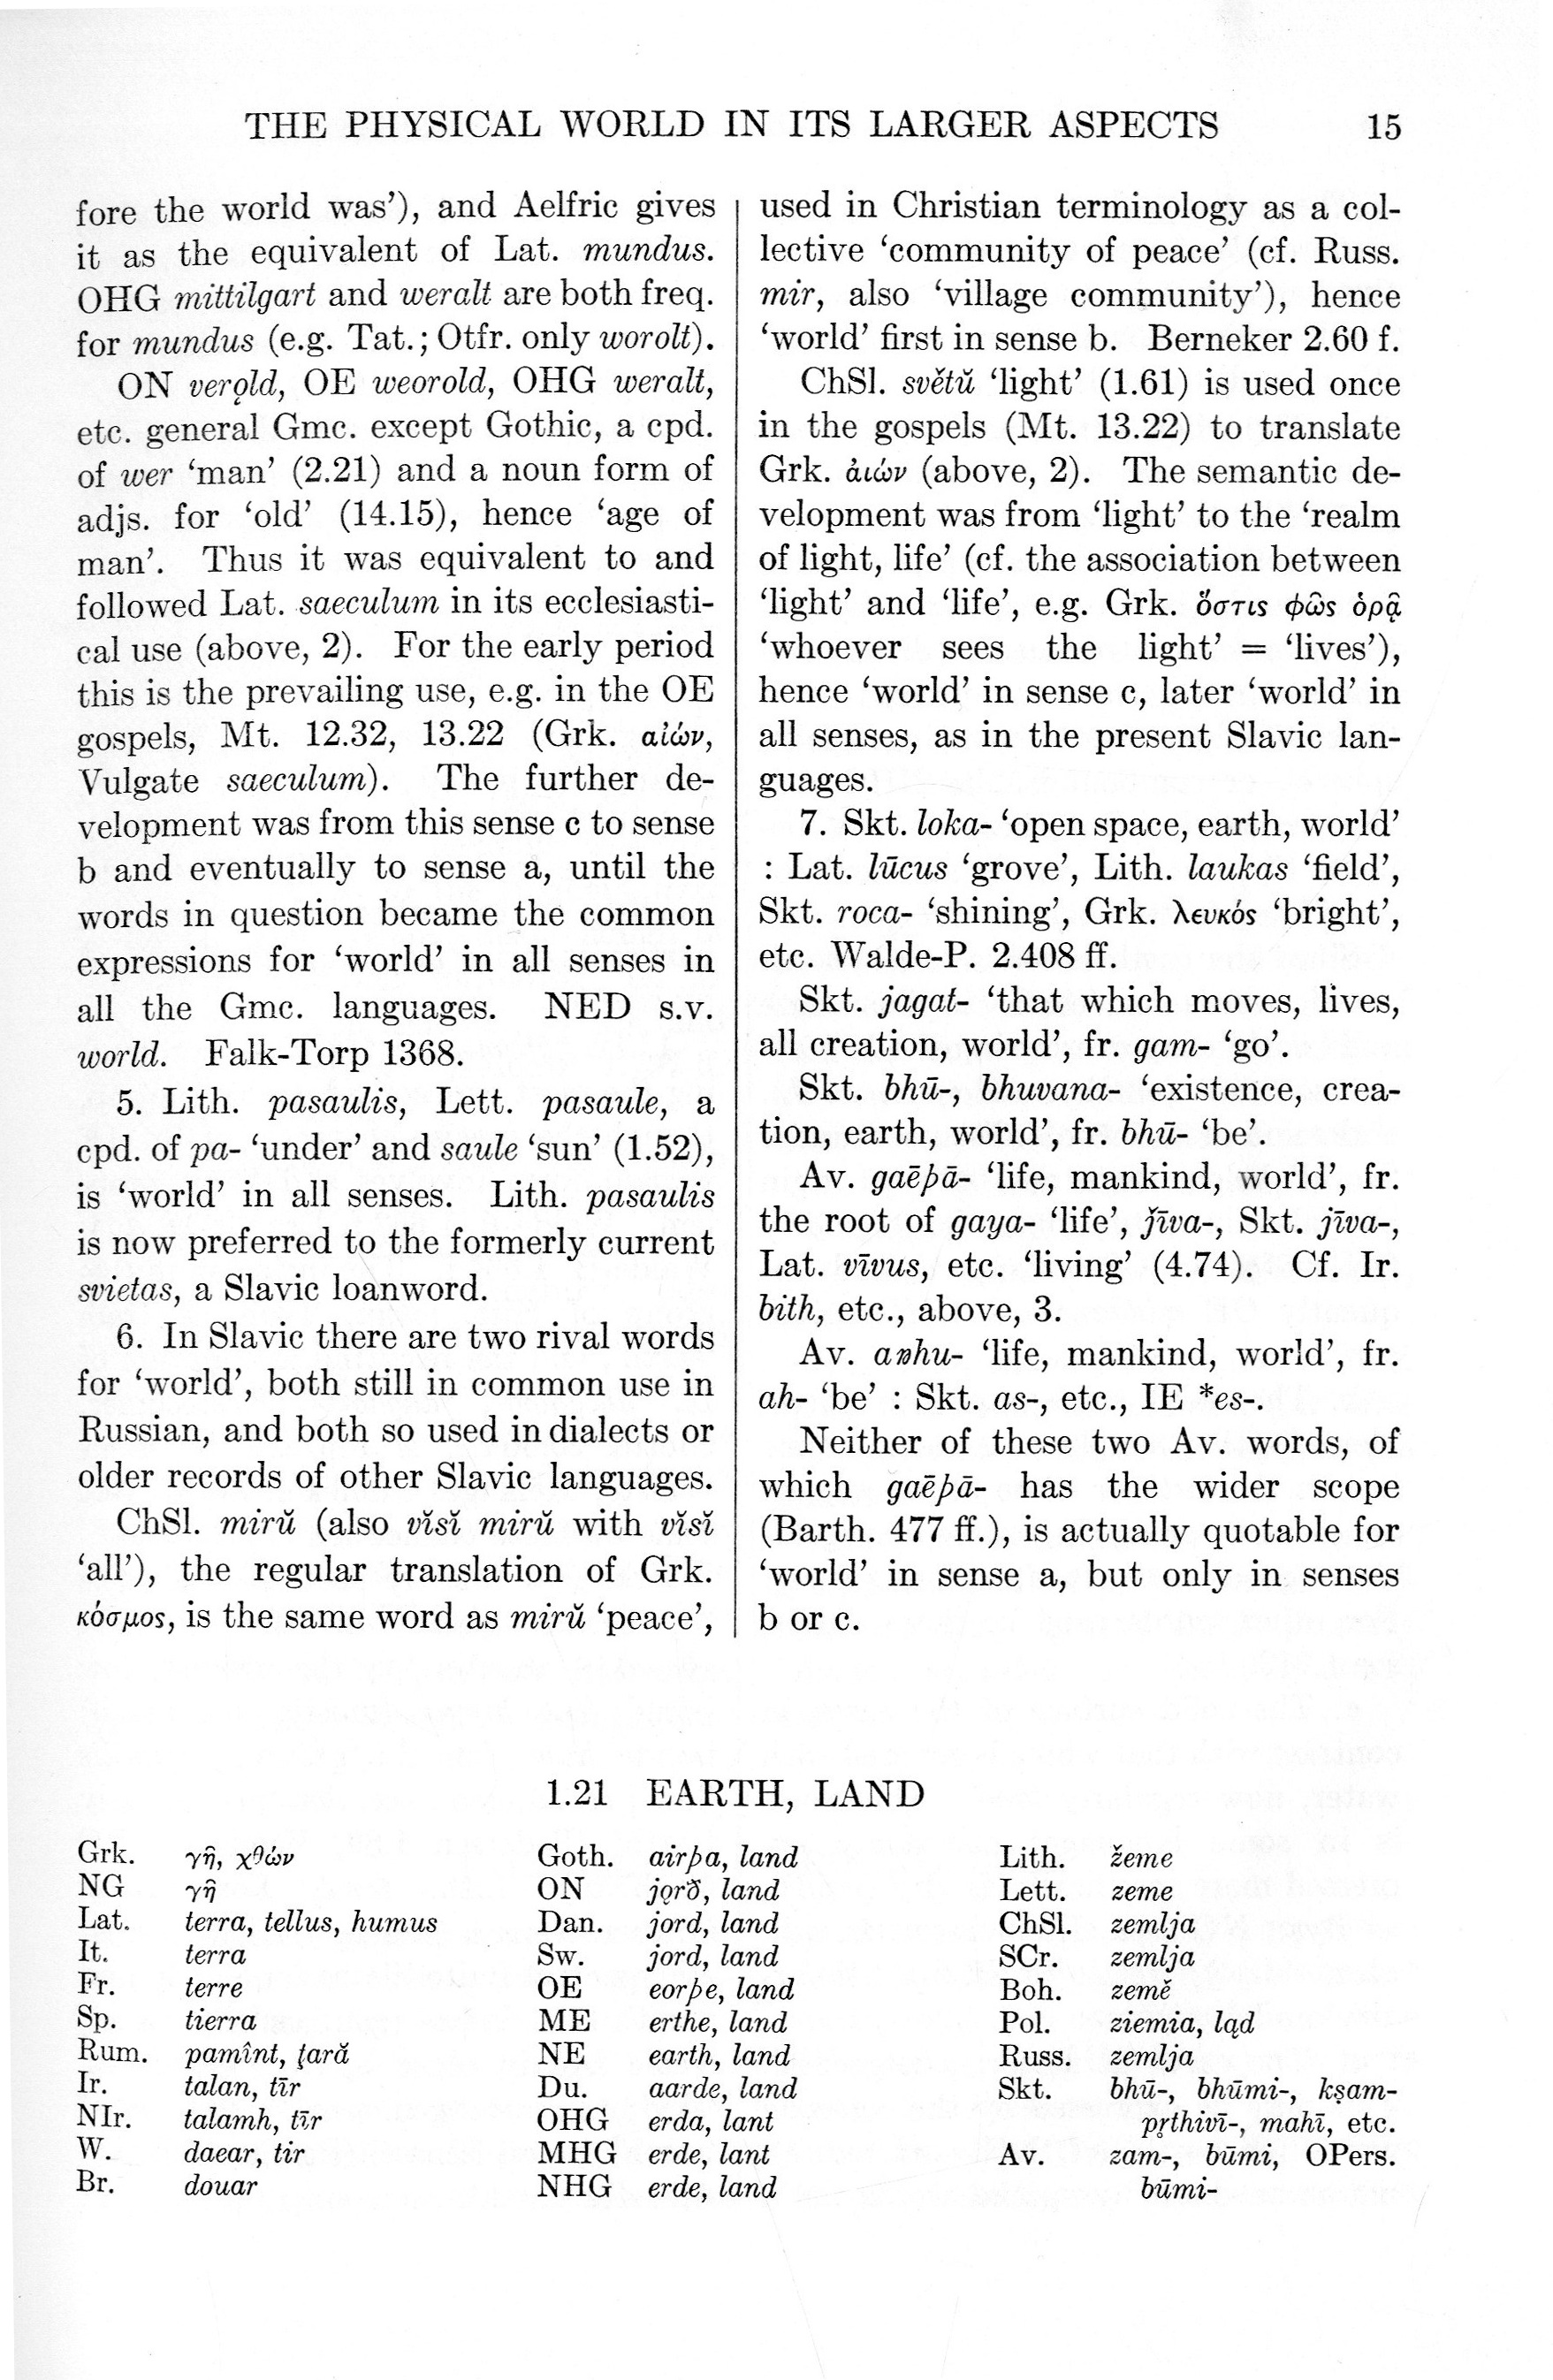
\includegraphics[width=\linewidth]{Stolk_thes-content/fig/thes/DSSPIEL-p0015.jpg}
\end{minipage}%
\begin{minipage}{.5\textwidth}
  \raggedleft
  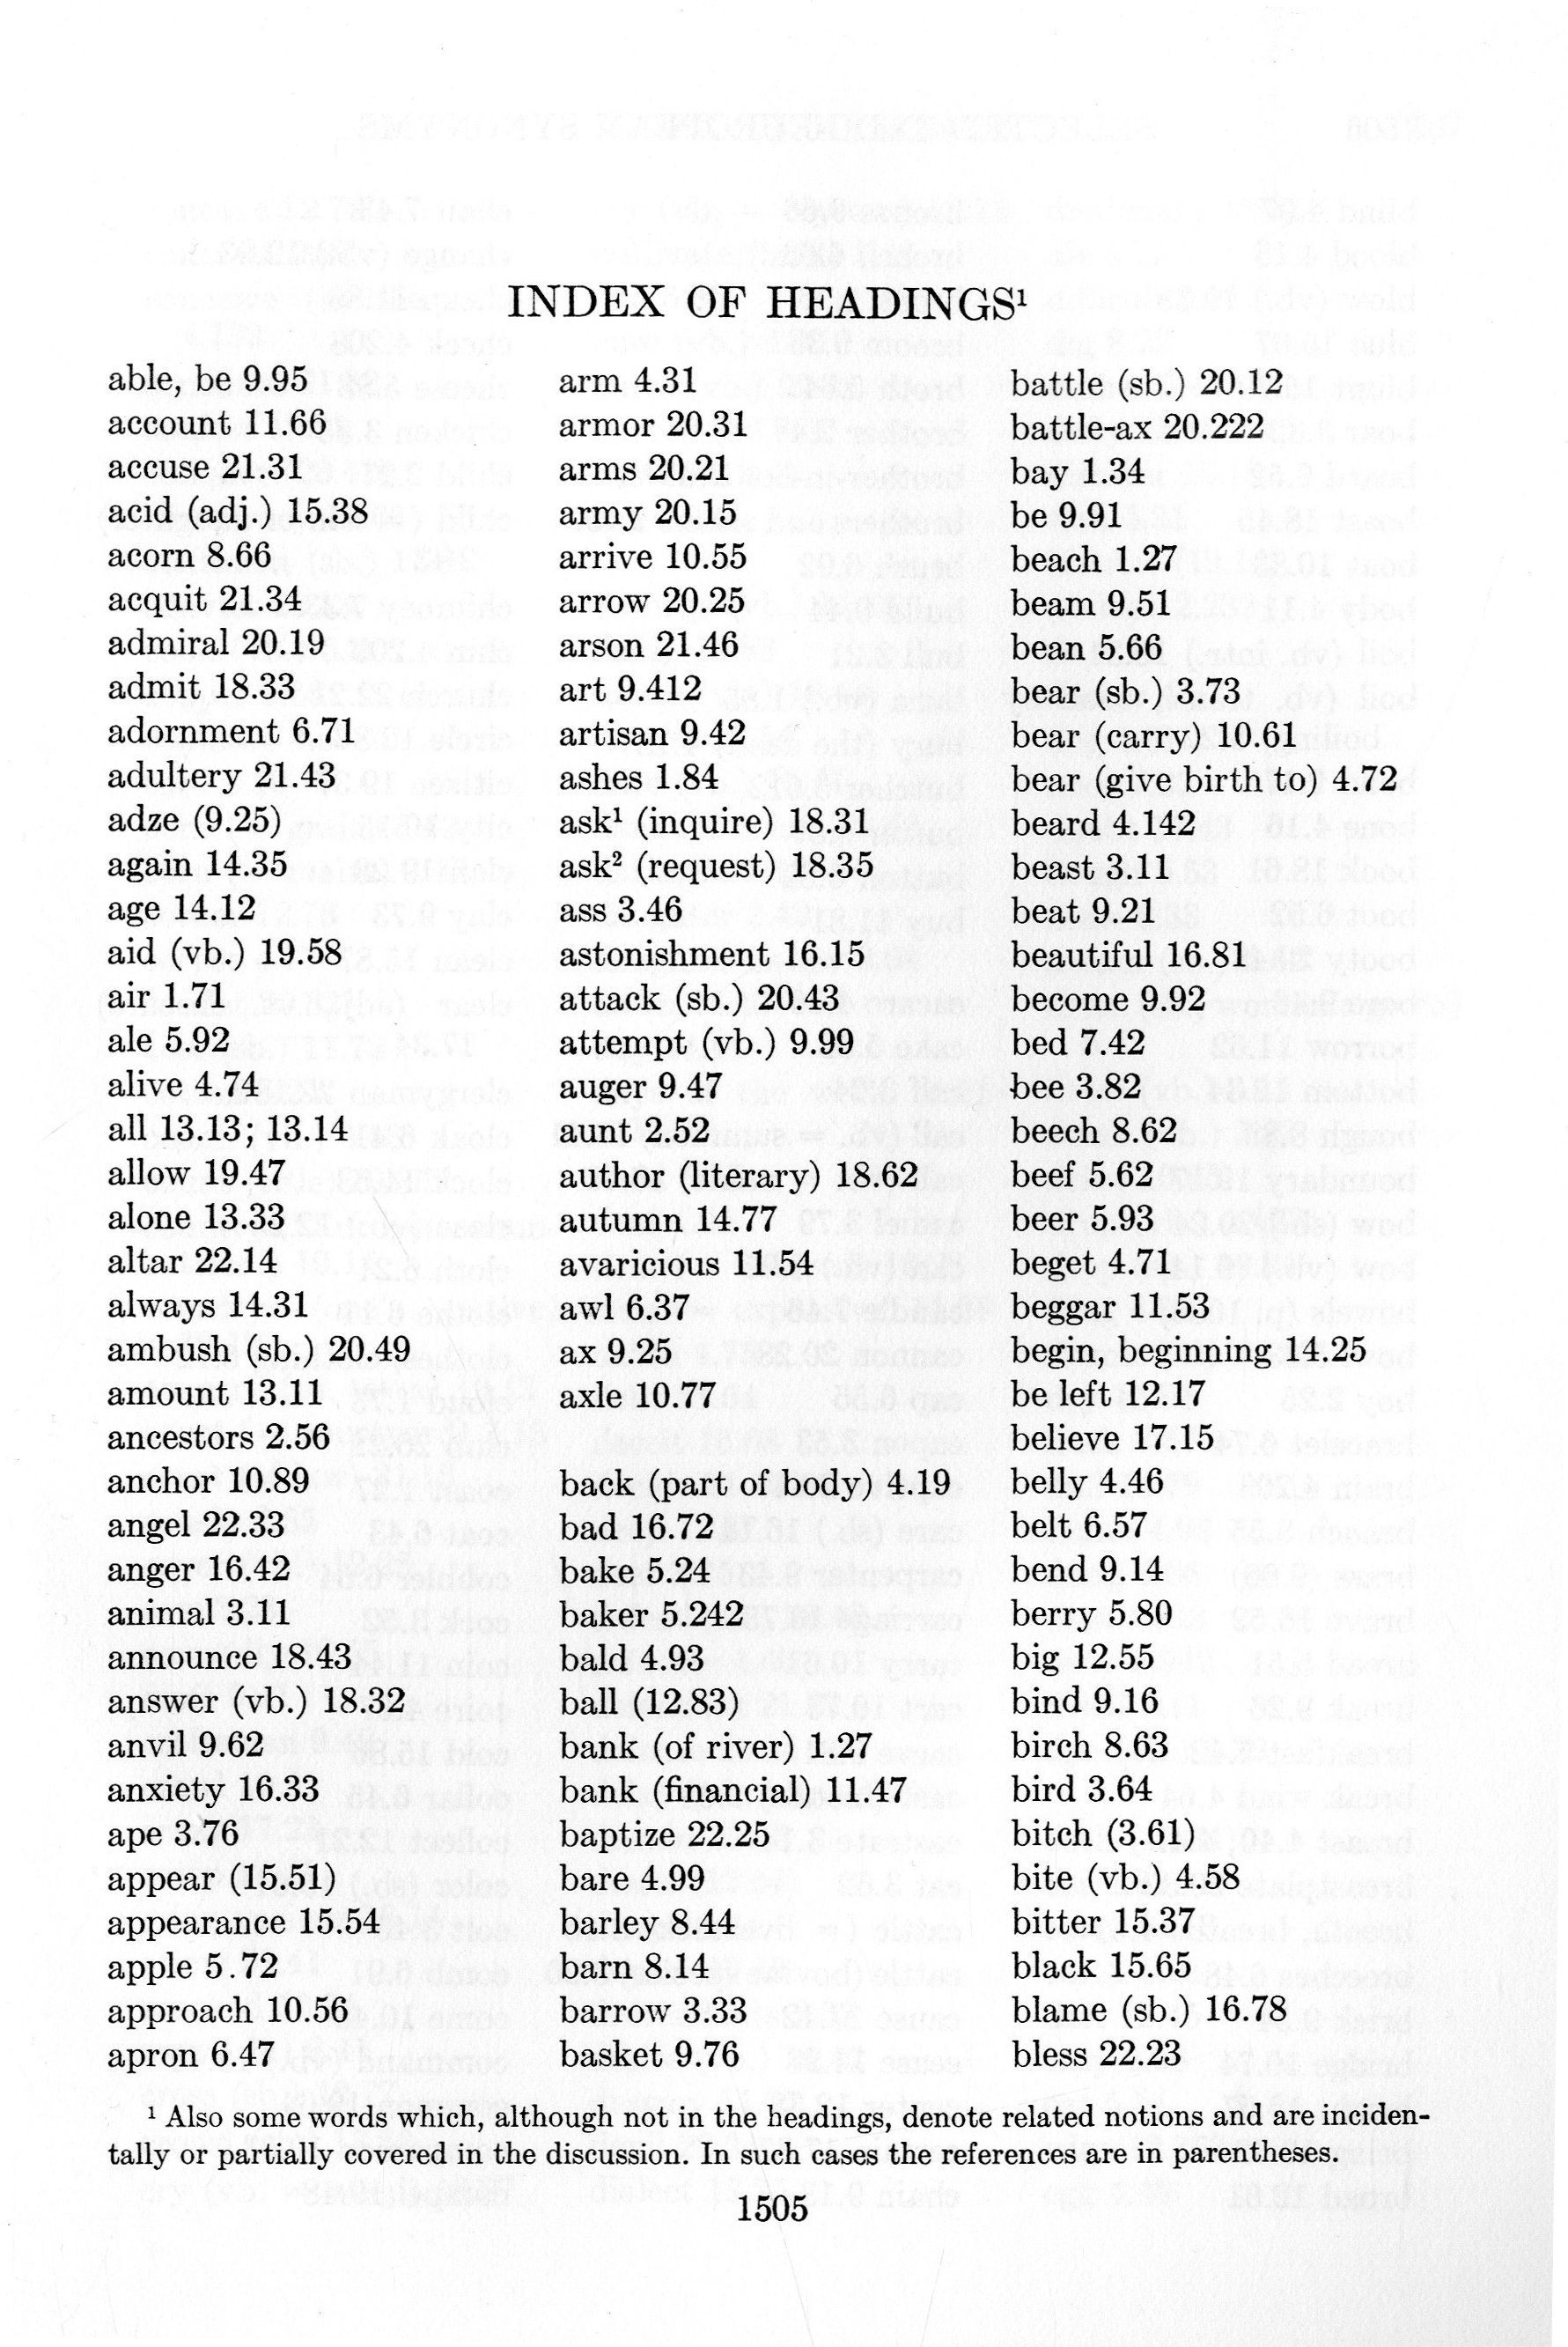
\includegraphics[width=\linewidth]{Stolk_thes-content/fig/thes/DSSPIEL-p1505.jpg}
\end{minipage}
  \caption{\textit{DSSPIEL}, p. 15 and p. 1505.}
  \label{fig:1.A:DSSPIEL}
\end{figure}

\noindent
\begin{figure}[htb]
  \centering
  \begin{minipage}{.5\textwidth}
    \raggedright
    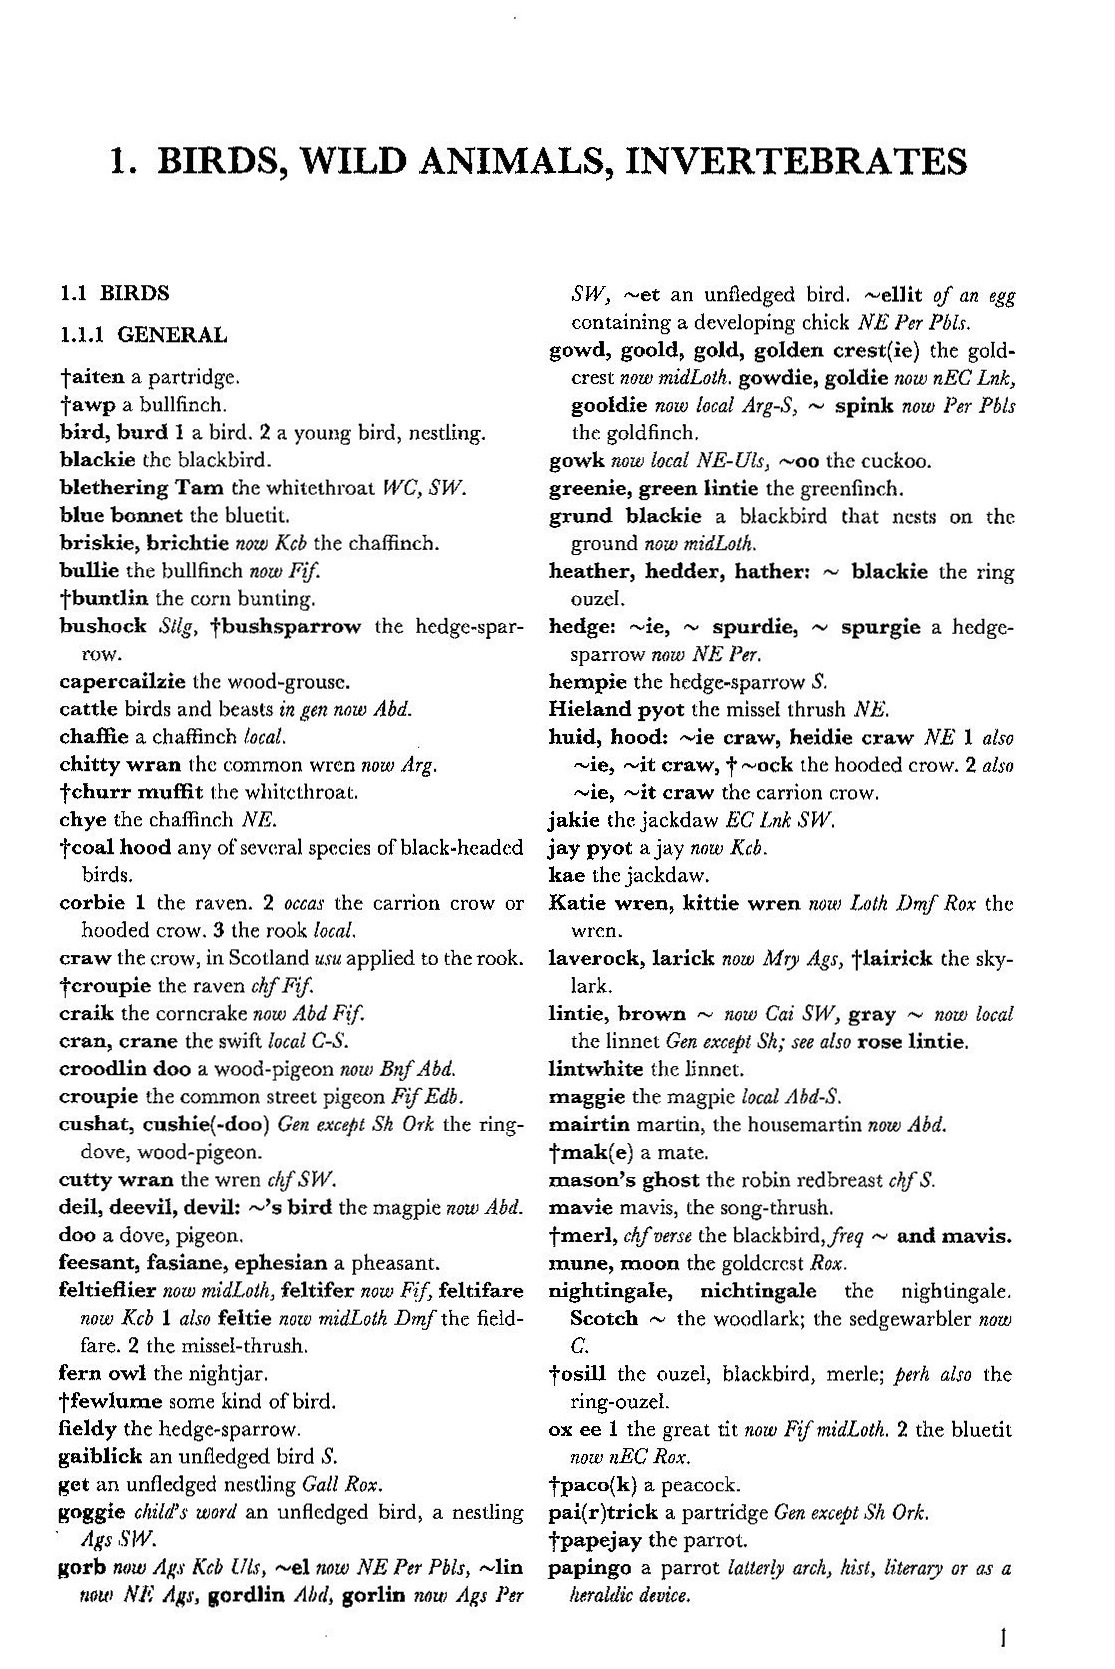
\includegraphics[width=\linewidth]{Stolk_thes-content/fig/thes/ScT-p001.jpg}
\end{minipage}%
\begin{minipage}{.5\textwidth}
  \raggedleft
  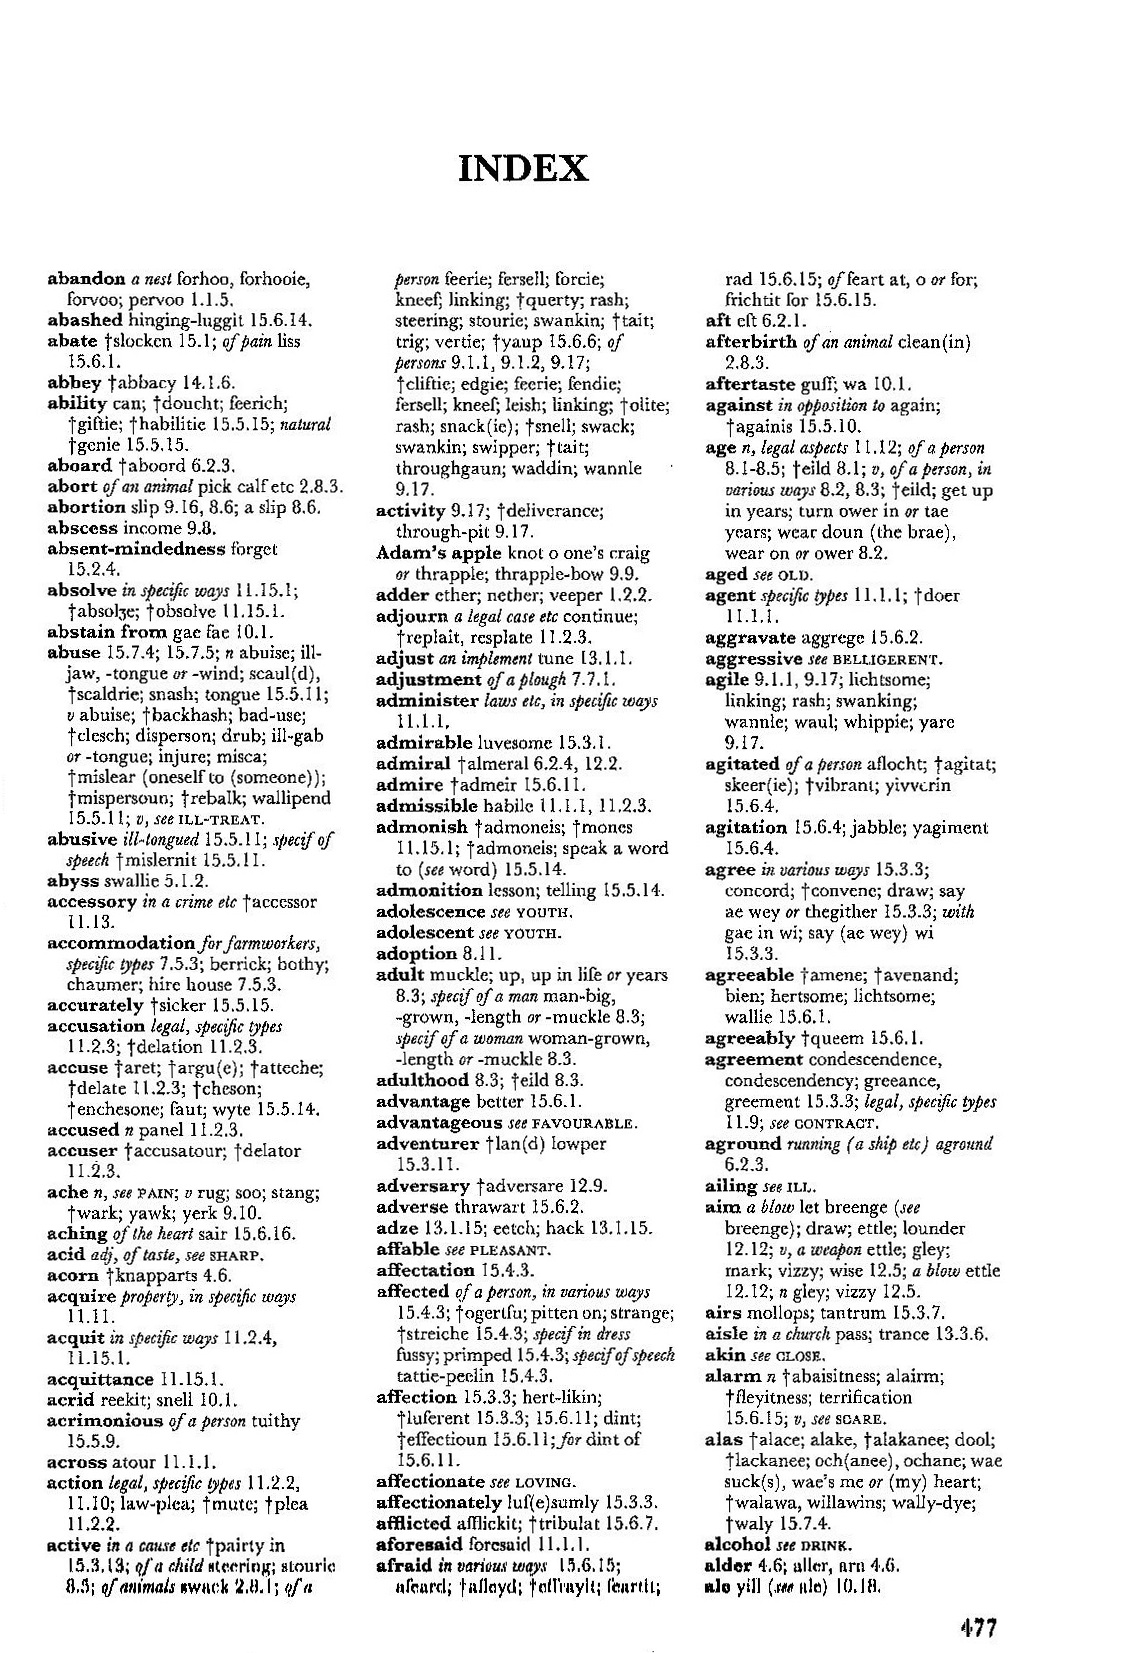
\includegraphics[width=\linewidth]{Stolk_thes-content/fig/thes/ScT-p477.jpg}
\end{minipage}
  \caption{\textit{ScT}, p. 1 and p. 477.}
  \label{fig:1.A:ScT}
\end{figure}

\noindent
\begin{figure}[htb]
  \centering
  \begin{minipage}{.5\textwidth}
    \raggedright
    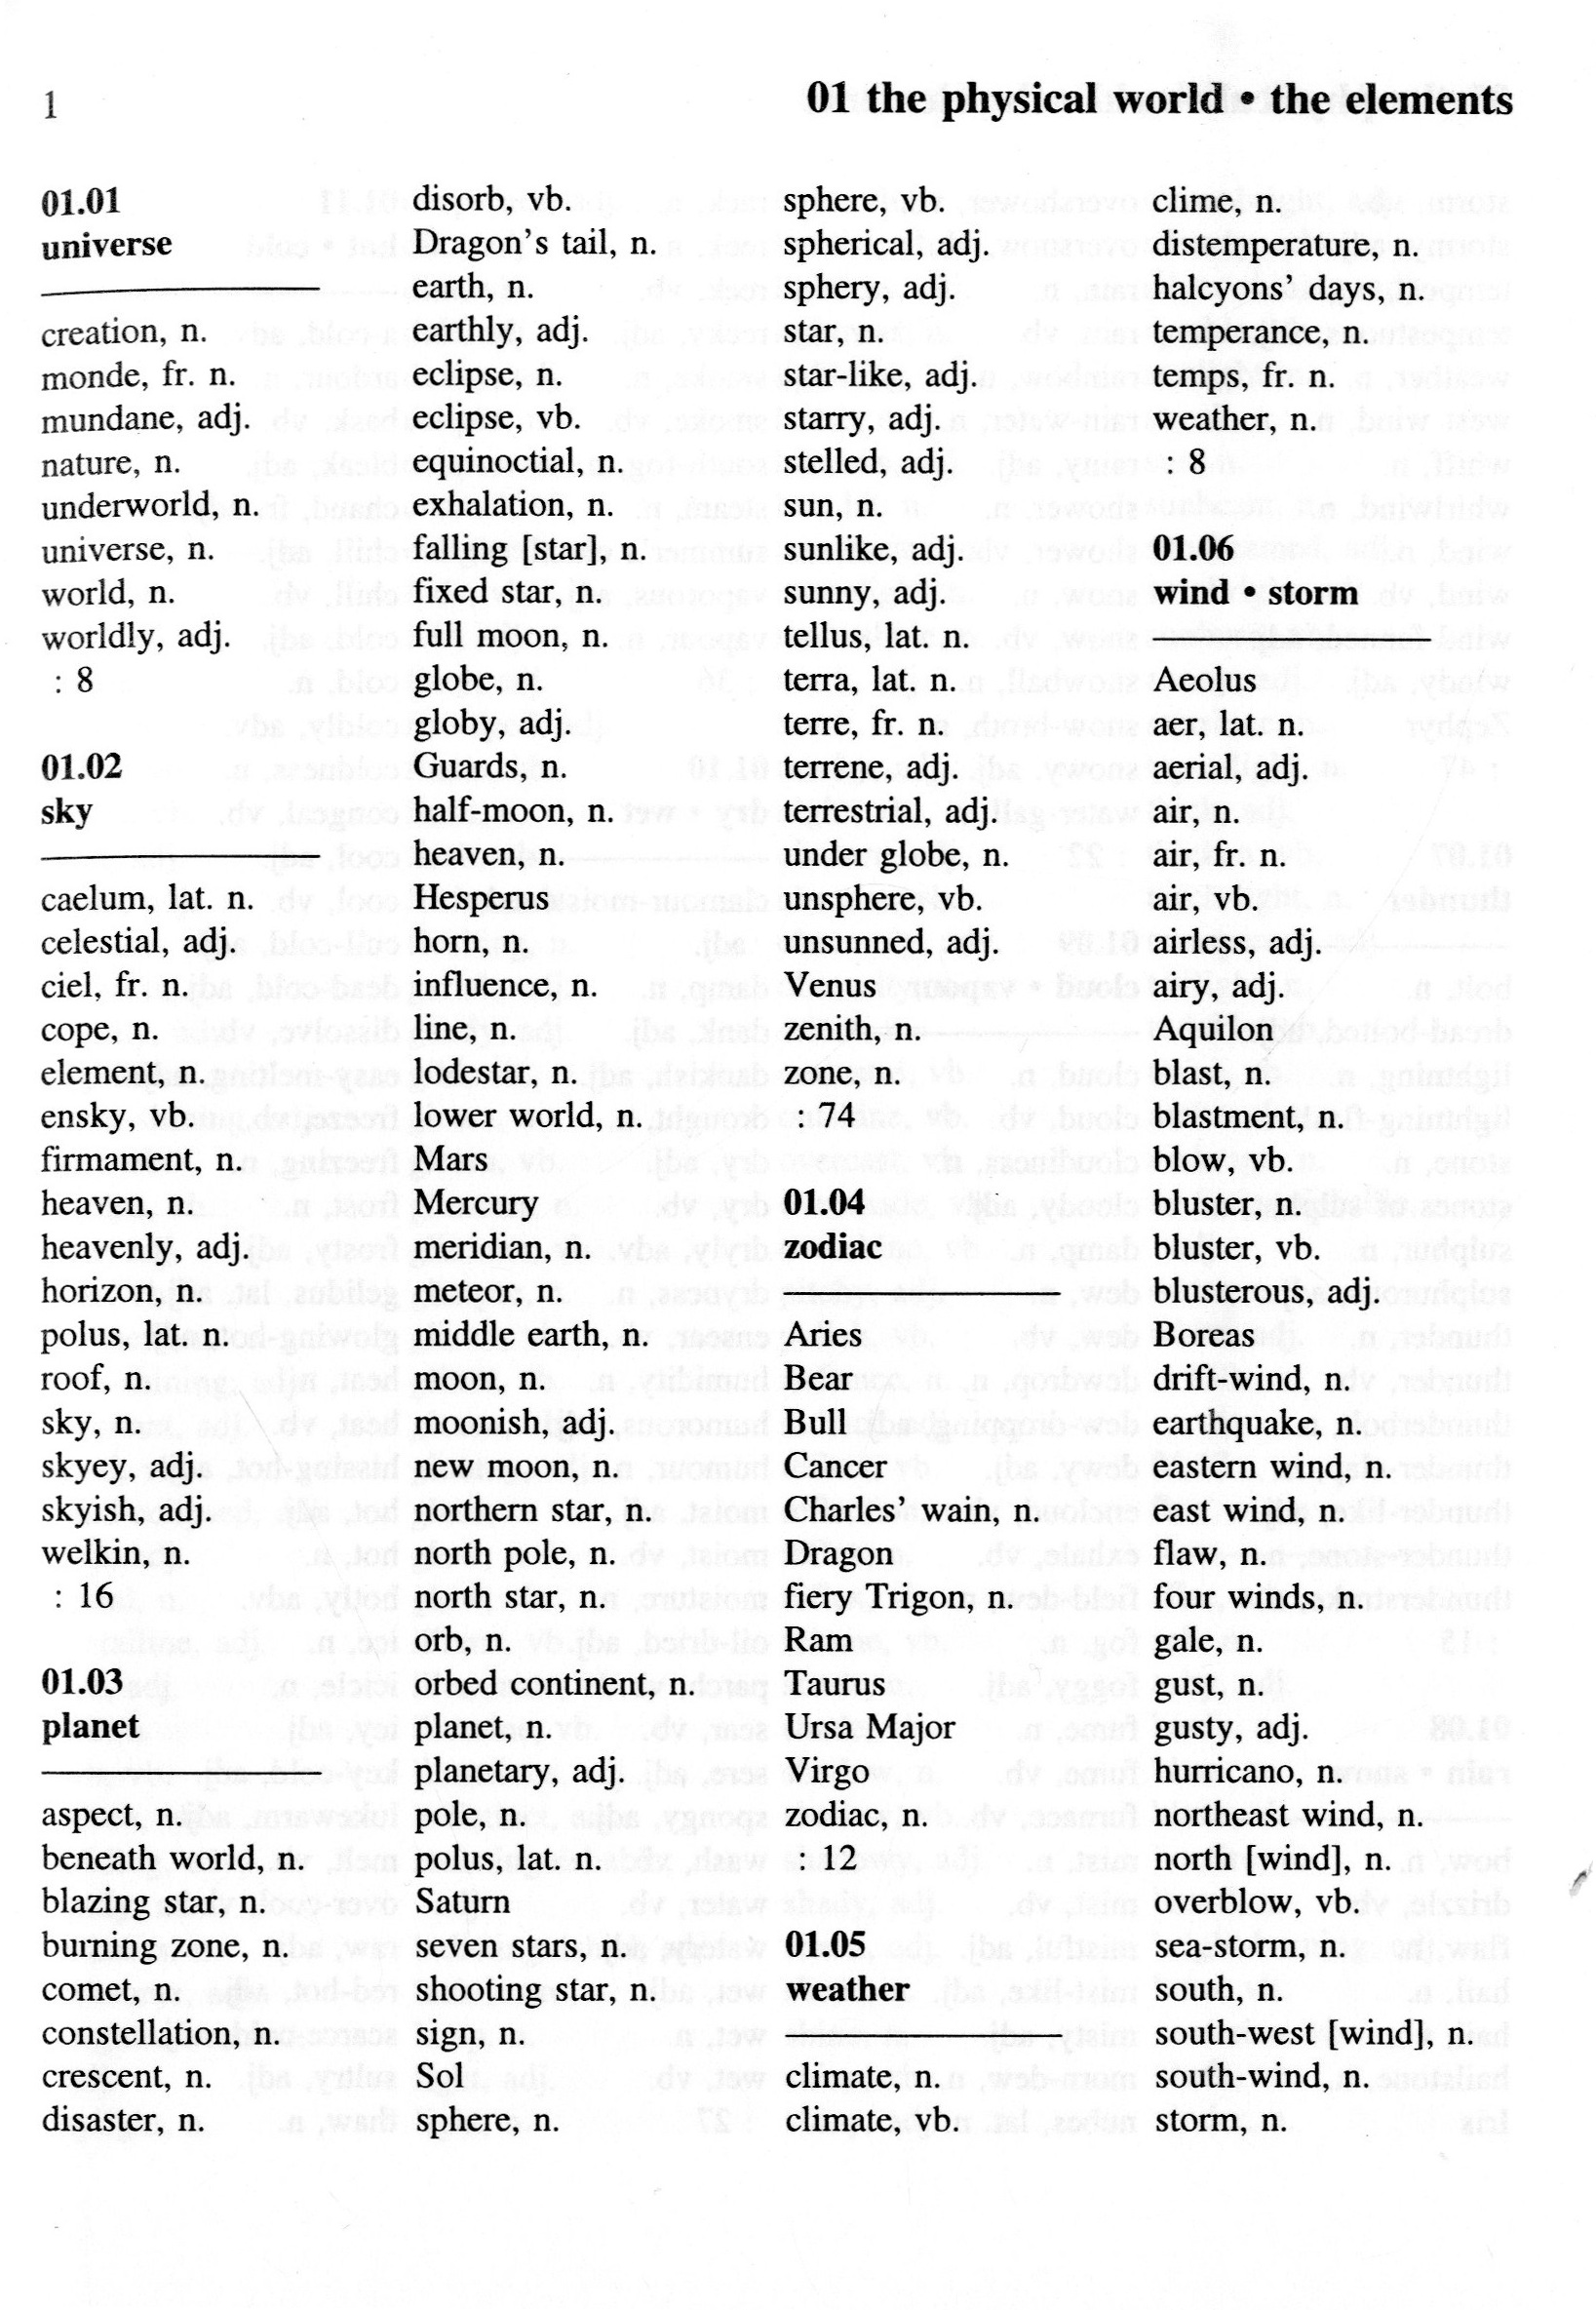
\includegraphics[width=\linewidth]{Stolk_thes-content/fig/thes/ShT-p001.jpg}
\end{minipage}%
\begin{minipage}{.5\textwidth}
  \raggedleft
  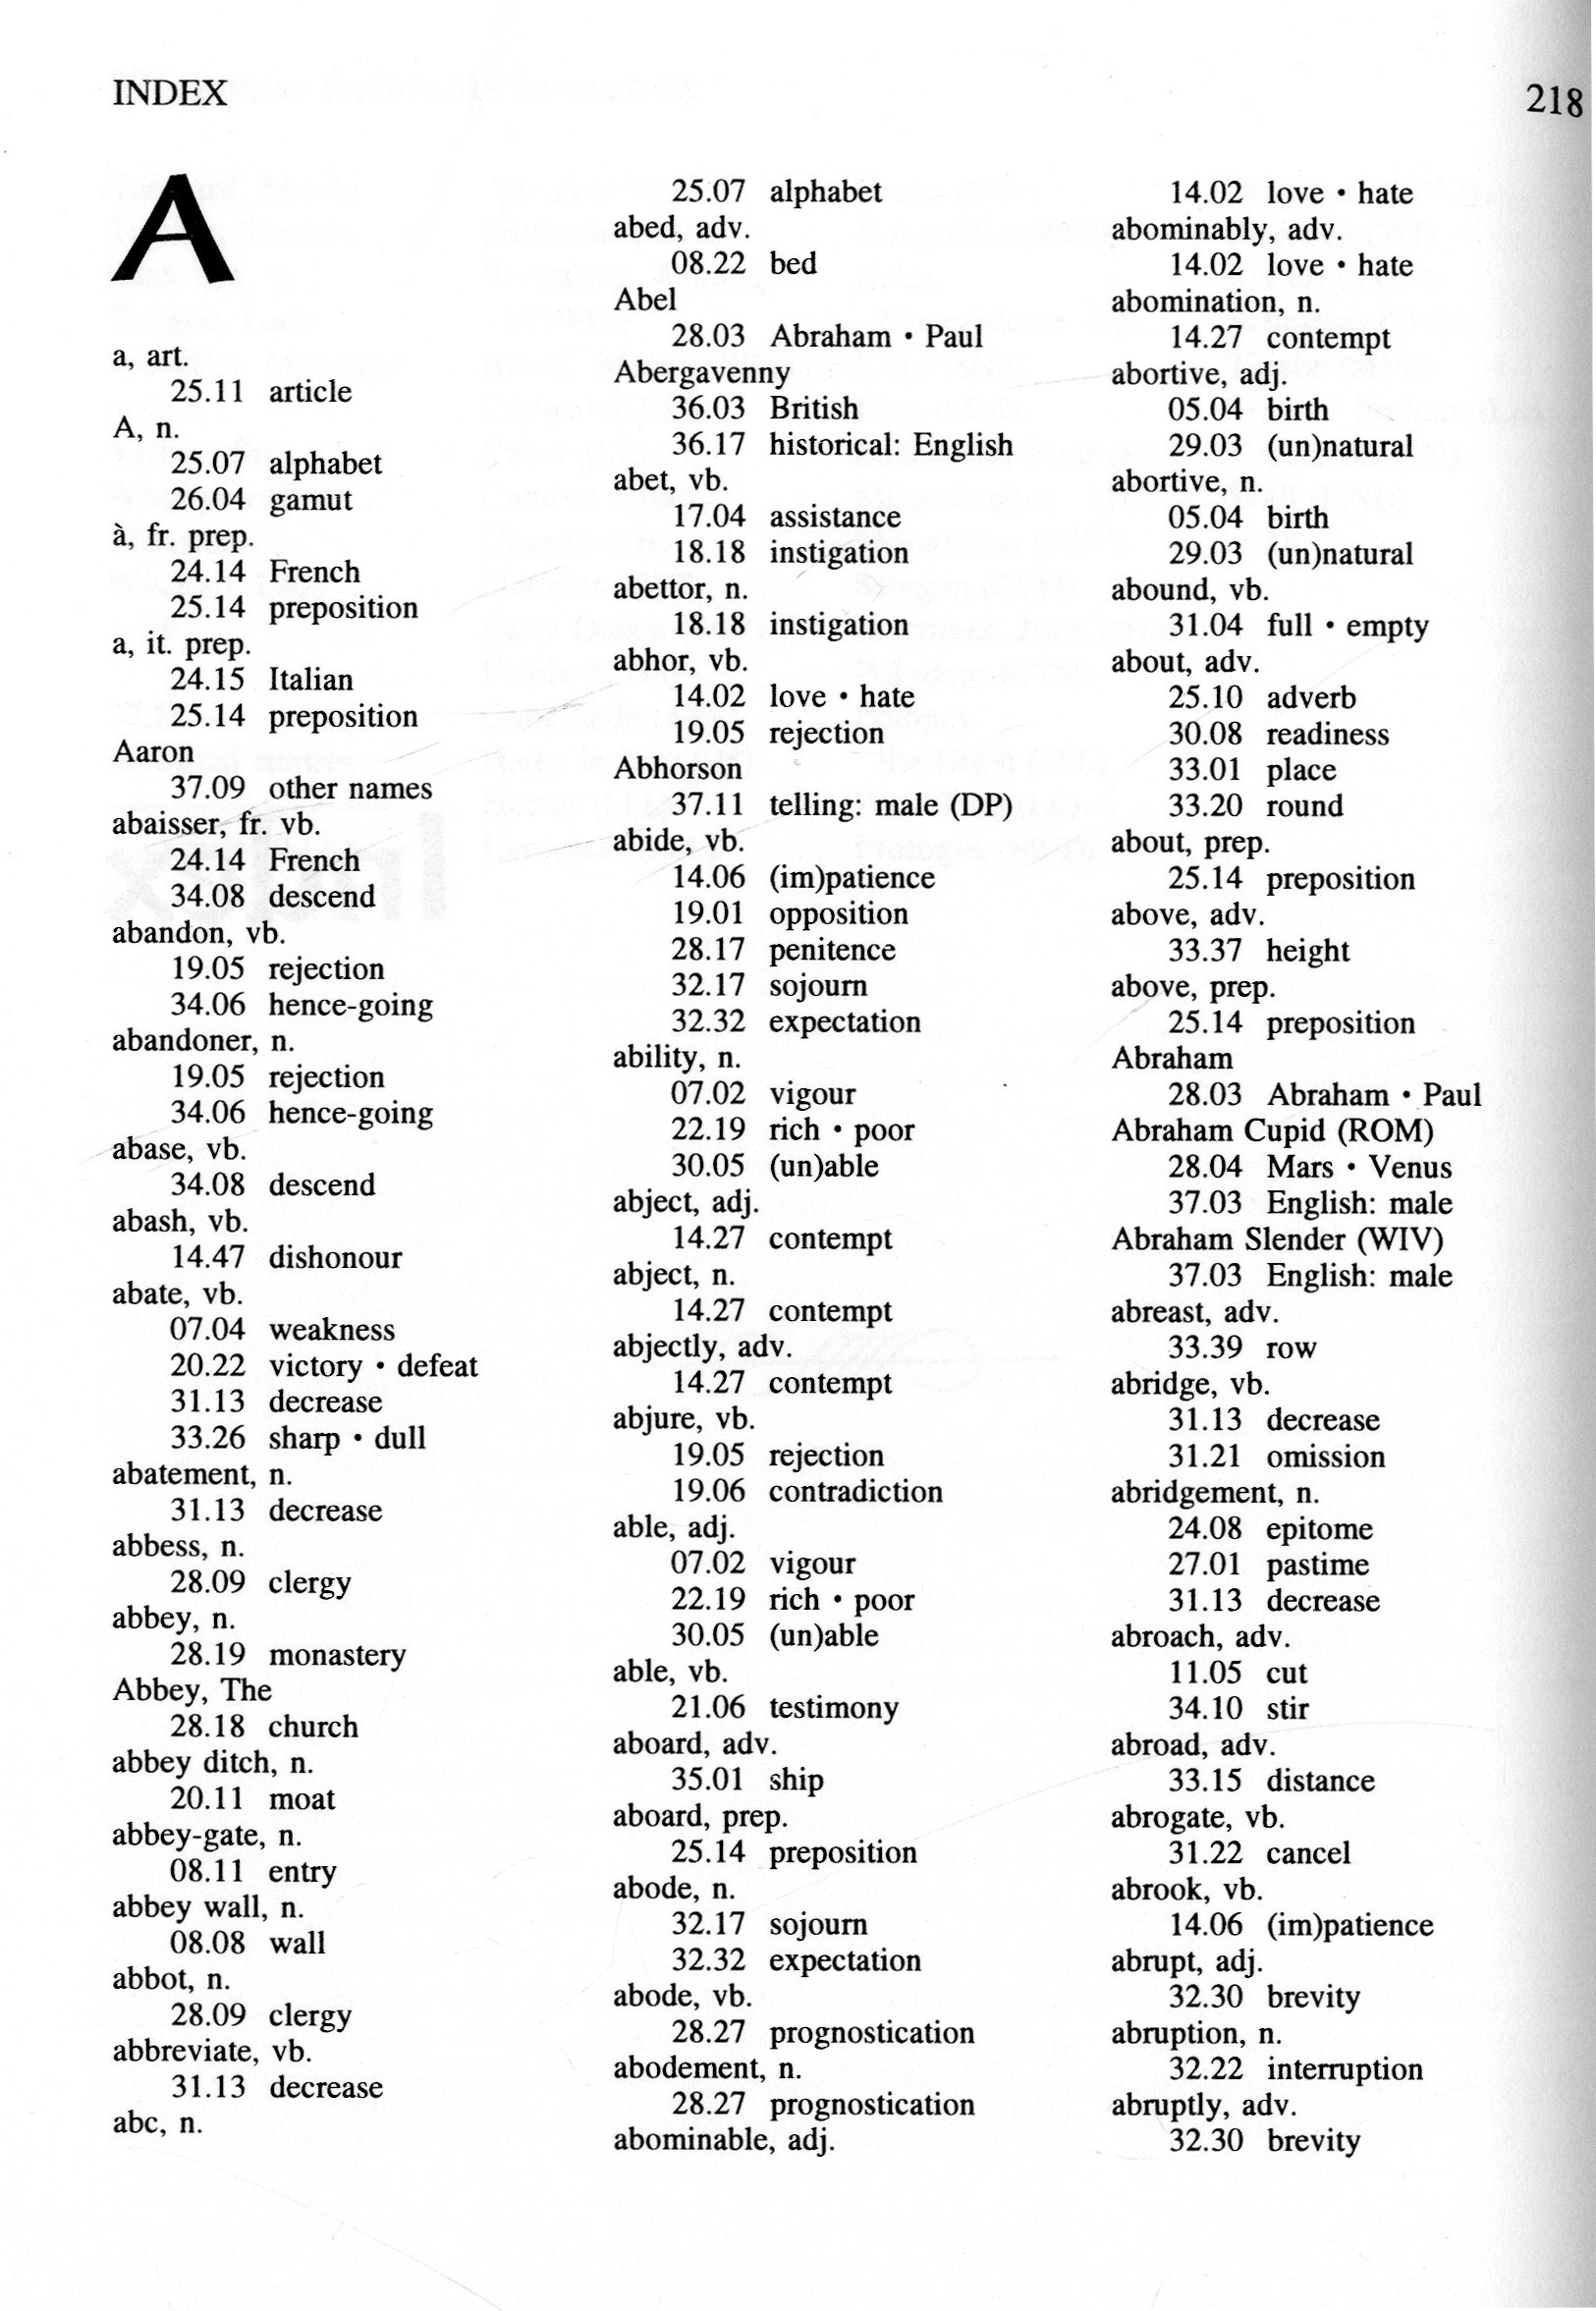
\includegraphics[width=\linewidth]{Stolk_thes-content/fig/thes/ShT-p218.jpg}
\end{minipage}
  \caption{\textit{ShT}, p. 1 and p. 218.}
  \label{fig:1.A:ShT}
\end{figure}

\noindent
\begin{figure}[htb]
  \centering
  \begin{minipage}{.5\textwidth}
    \raggedright
    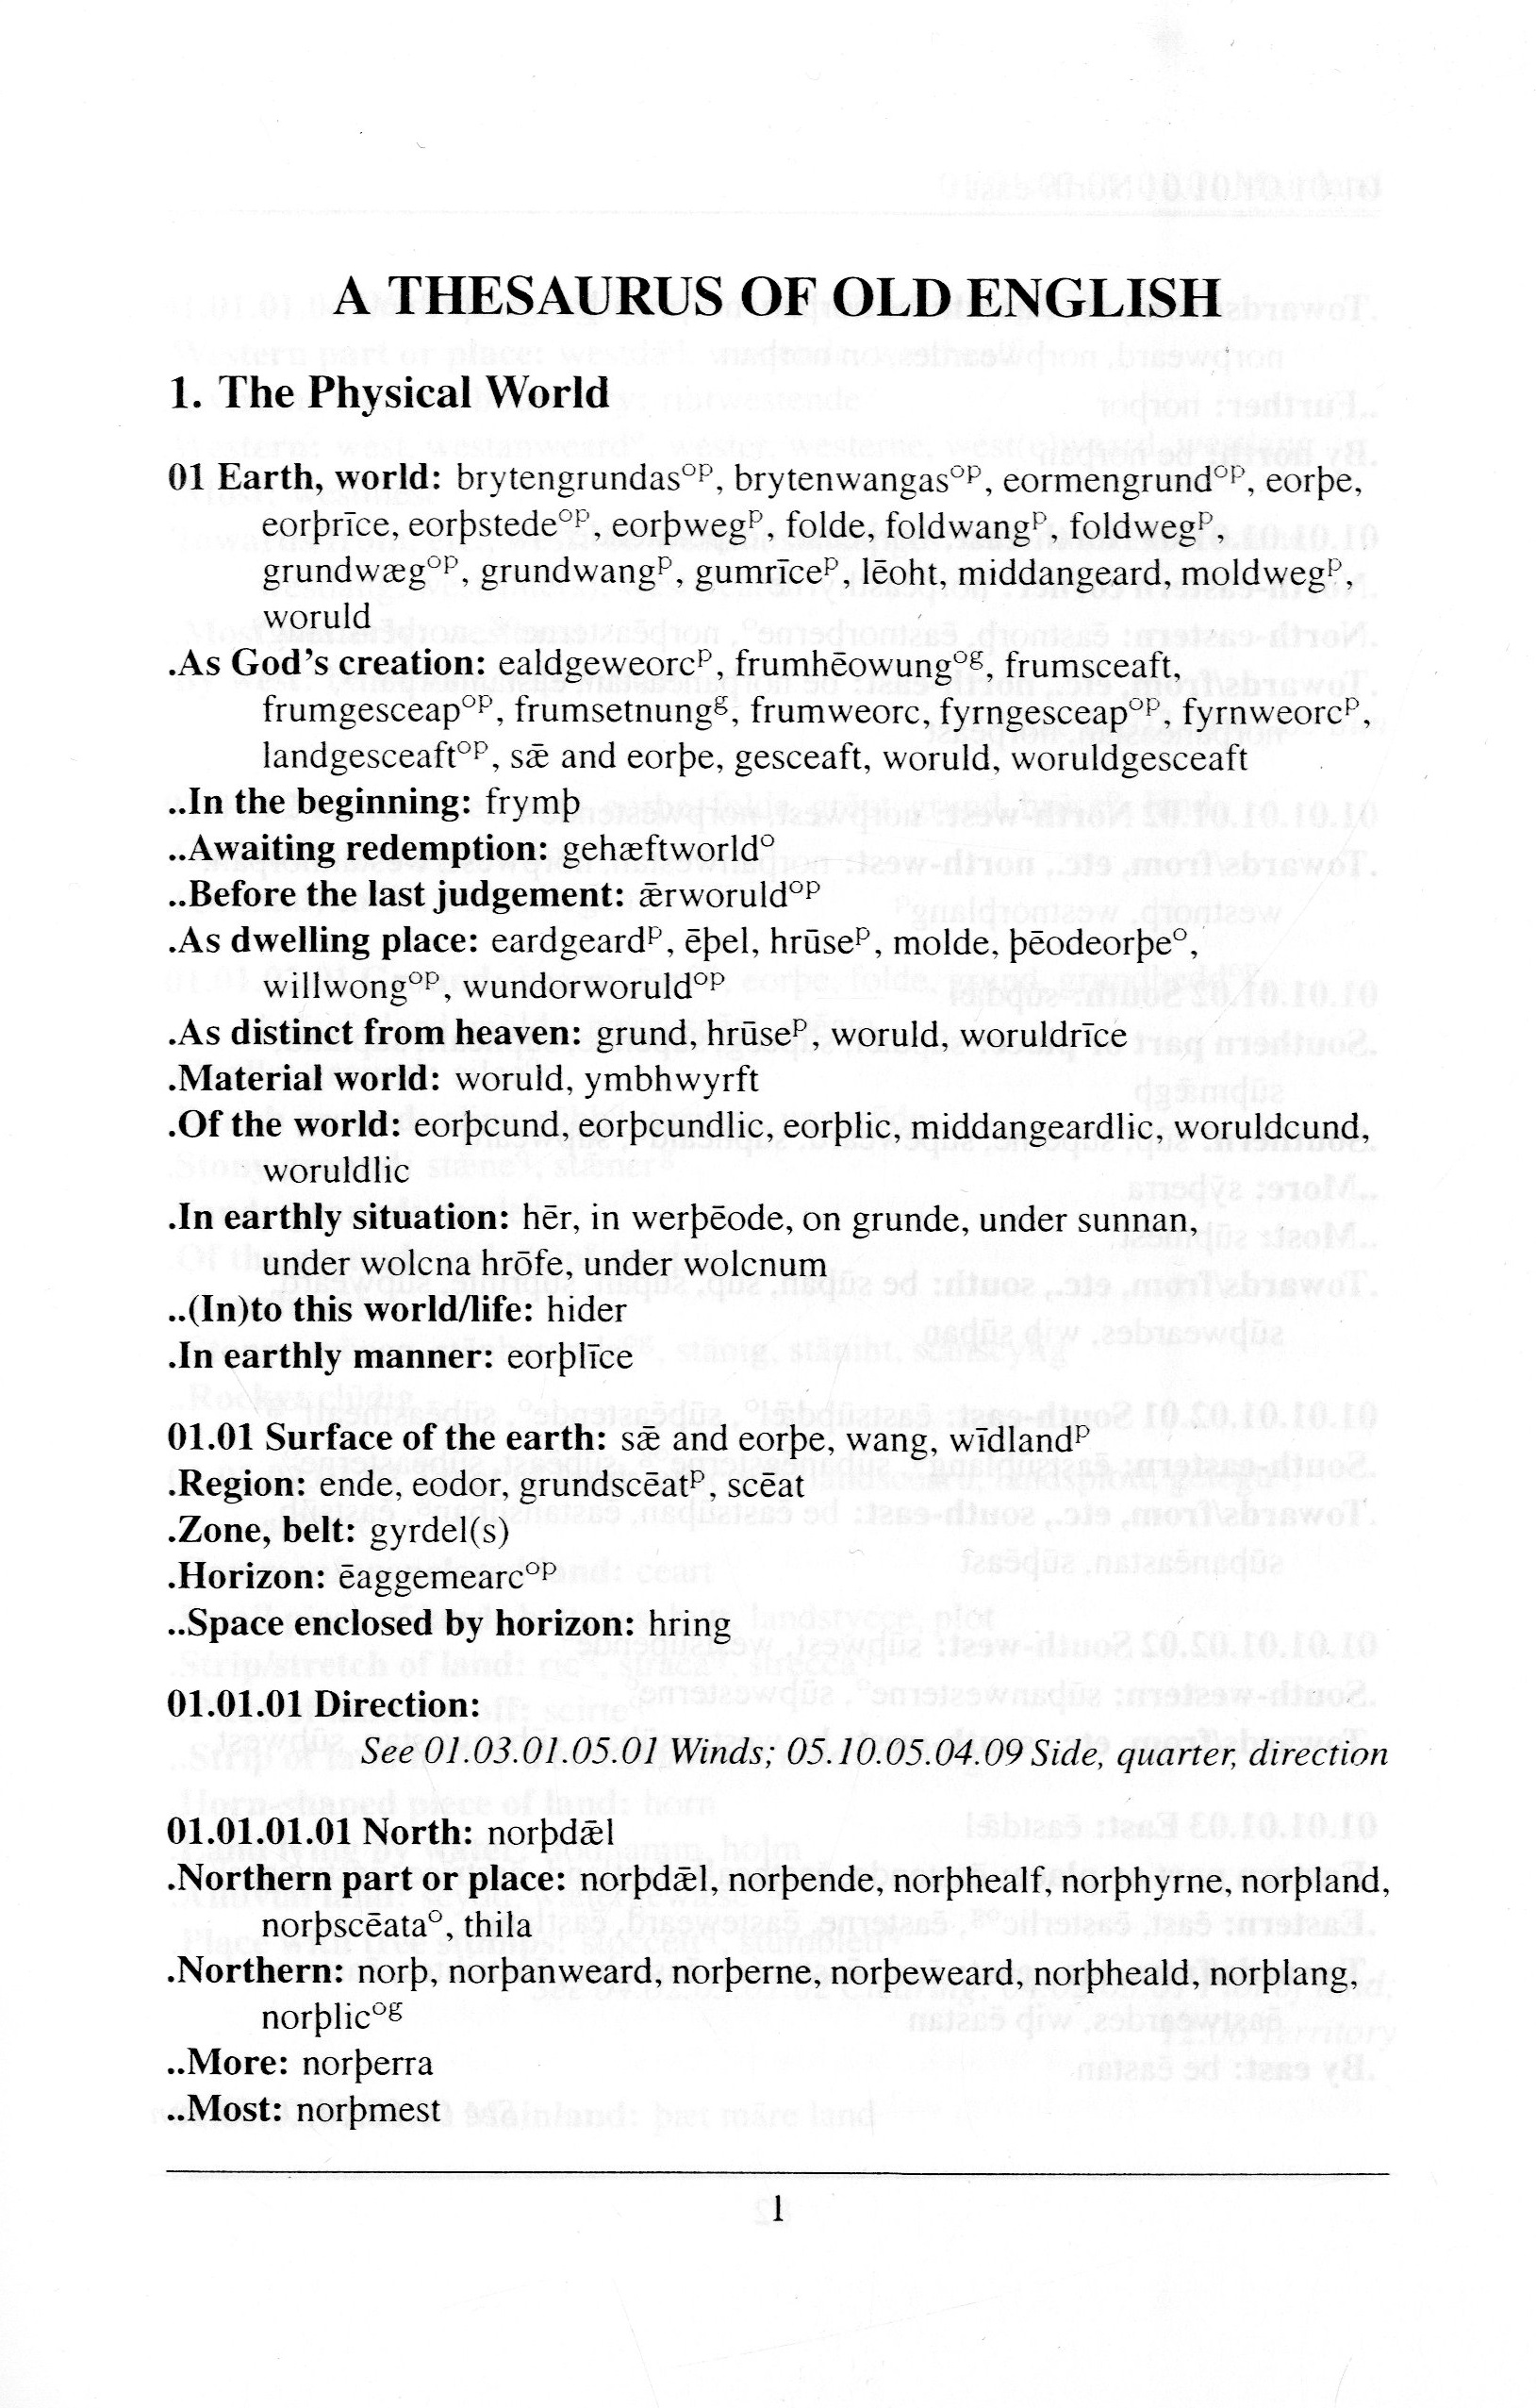
\includegraphics[width=\linewidth]{Stolk_thes-content/fig/thes/TOE2-p001.jpg}
\end{minipage}%
\begin{minipage}{.5\textwidth}
  \raggedleft
  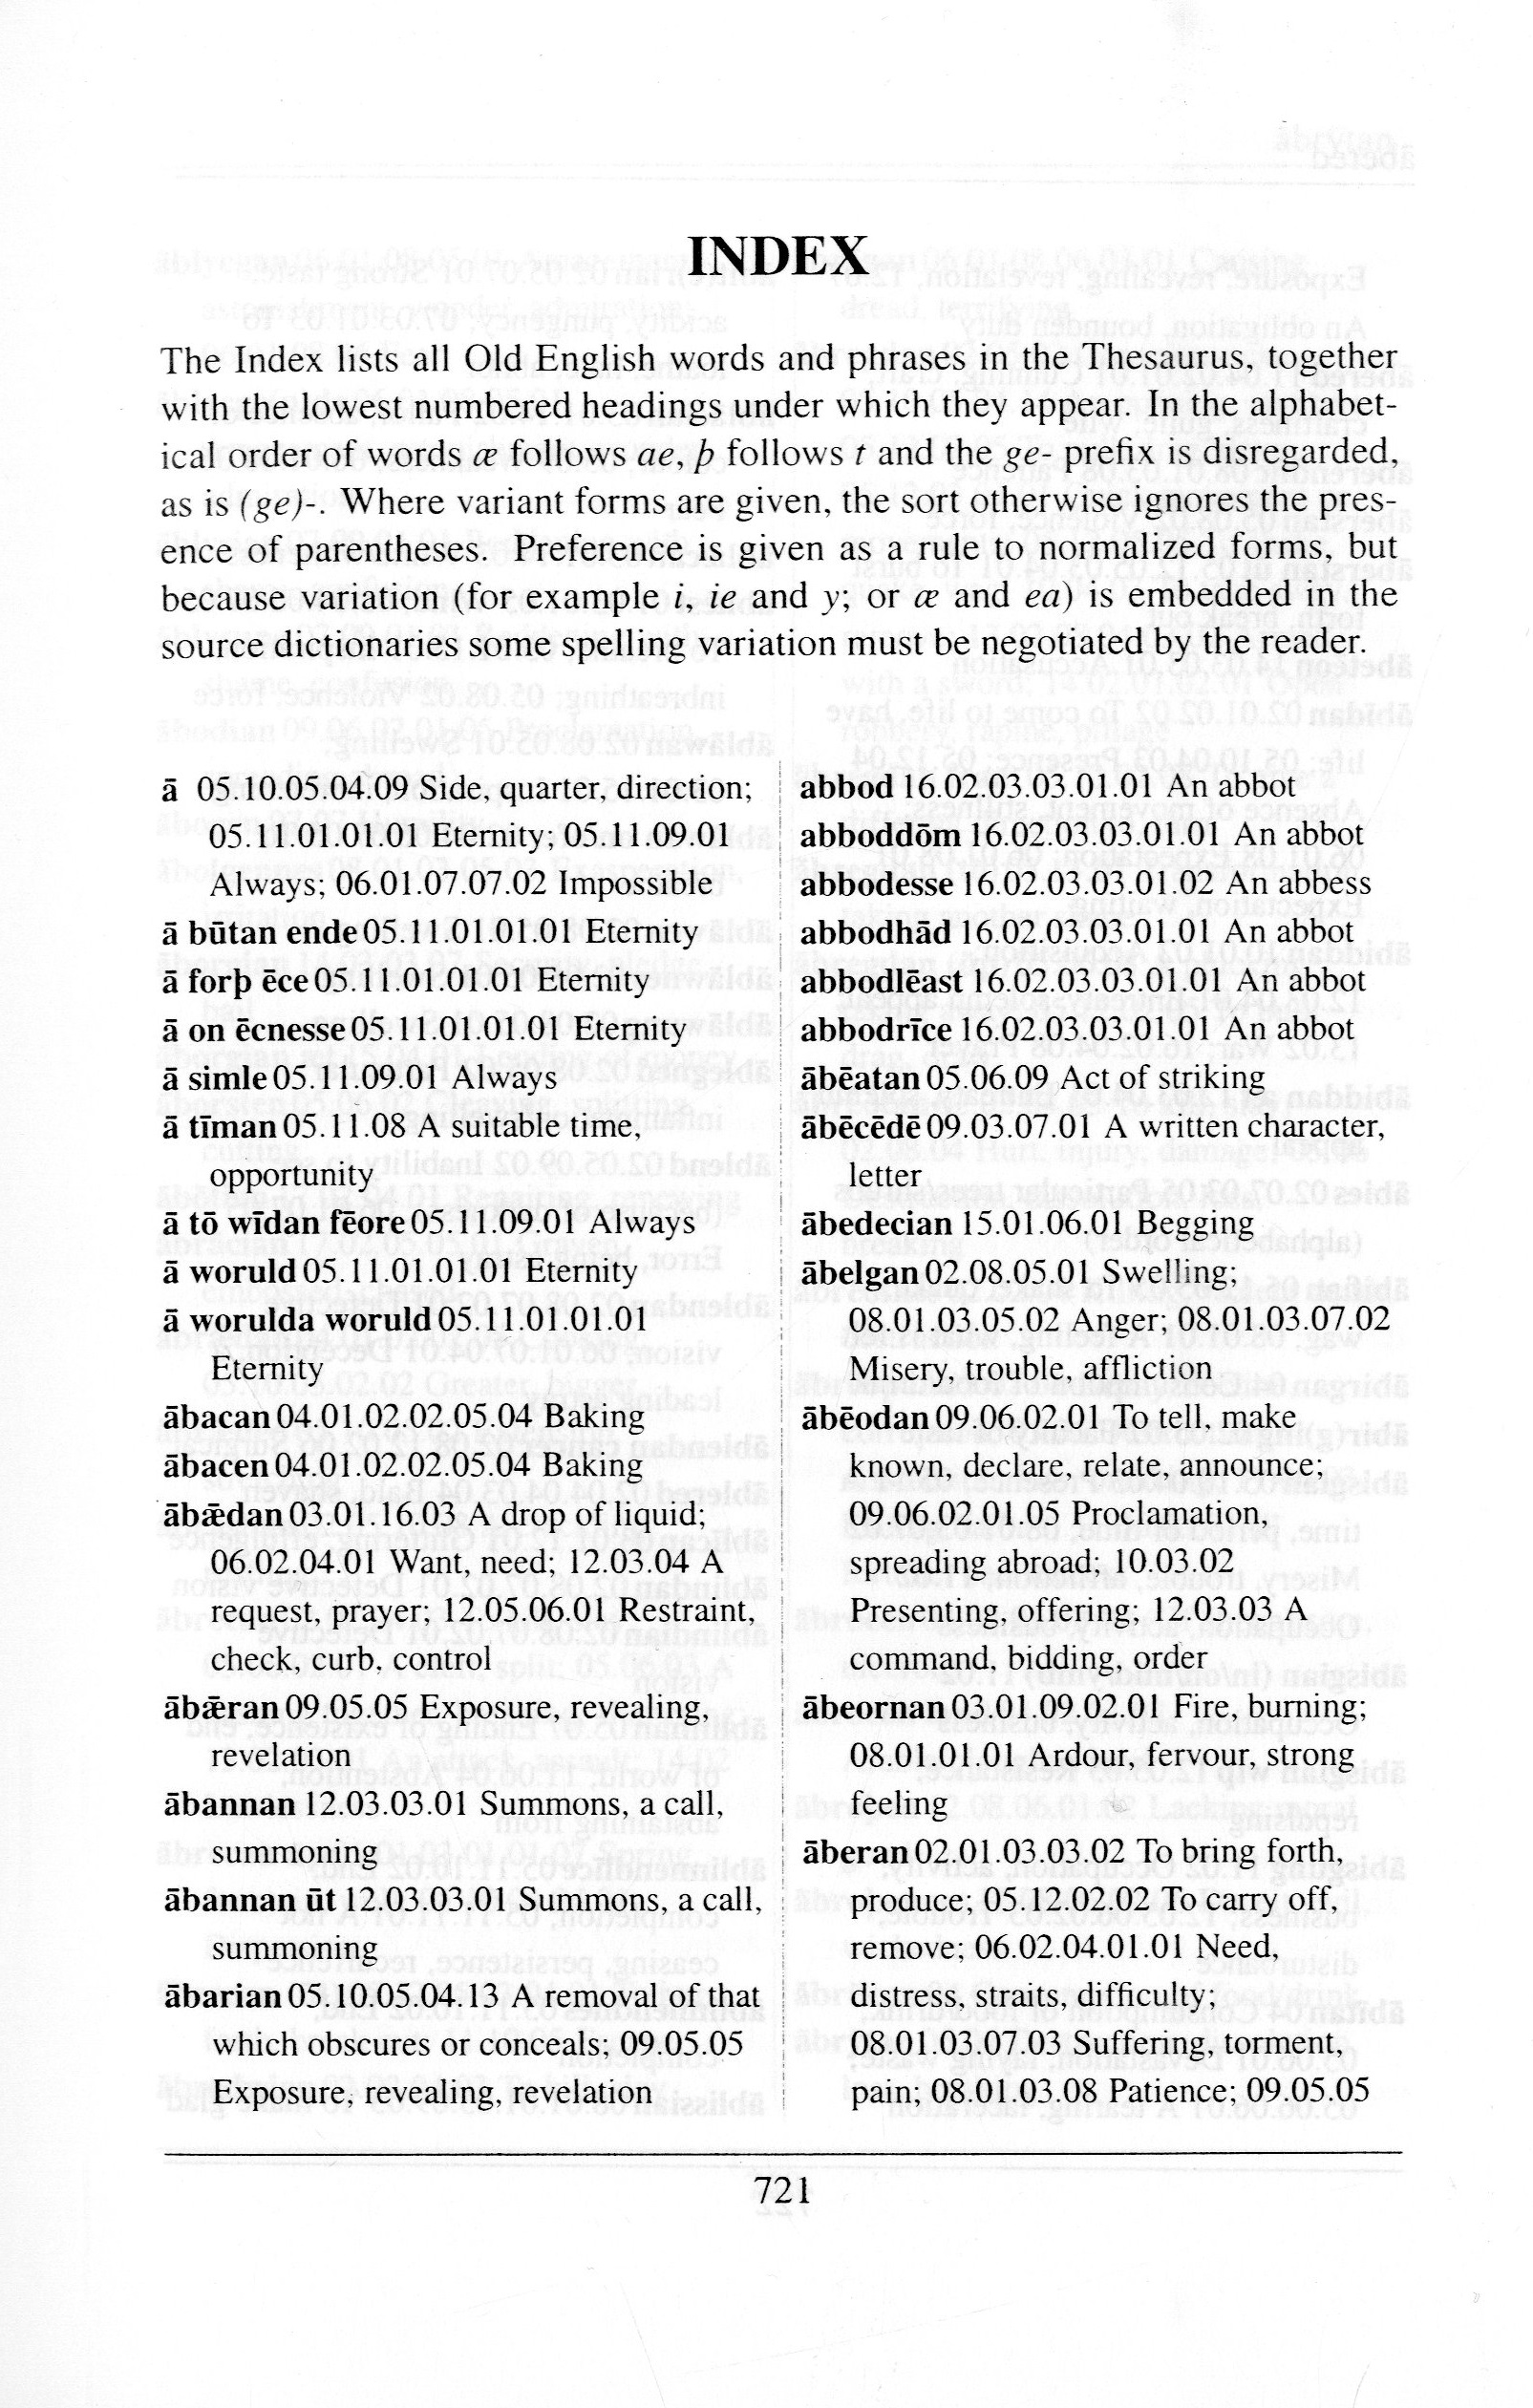
\includegraphics[width=\linewidth]{Stolk_thes-content/fig/thes/TOE2-p721.jpg}
\end{minipage}
  \caption{\textit{TOE2}, p. 1 and p. 721.}
  \label{fig:1.A:TOE2}
\end{figure}

% TOE4

\noindent
\begin{figure}[htb]
  \centering
  \begin{minipage}{.5\textwidth}
    \raggedright
    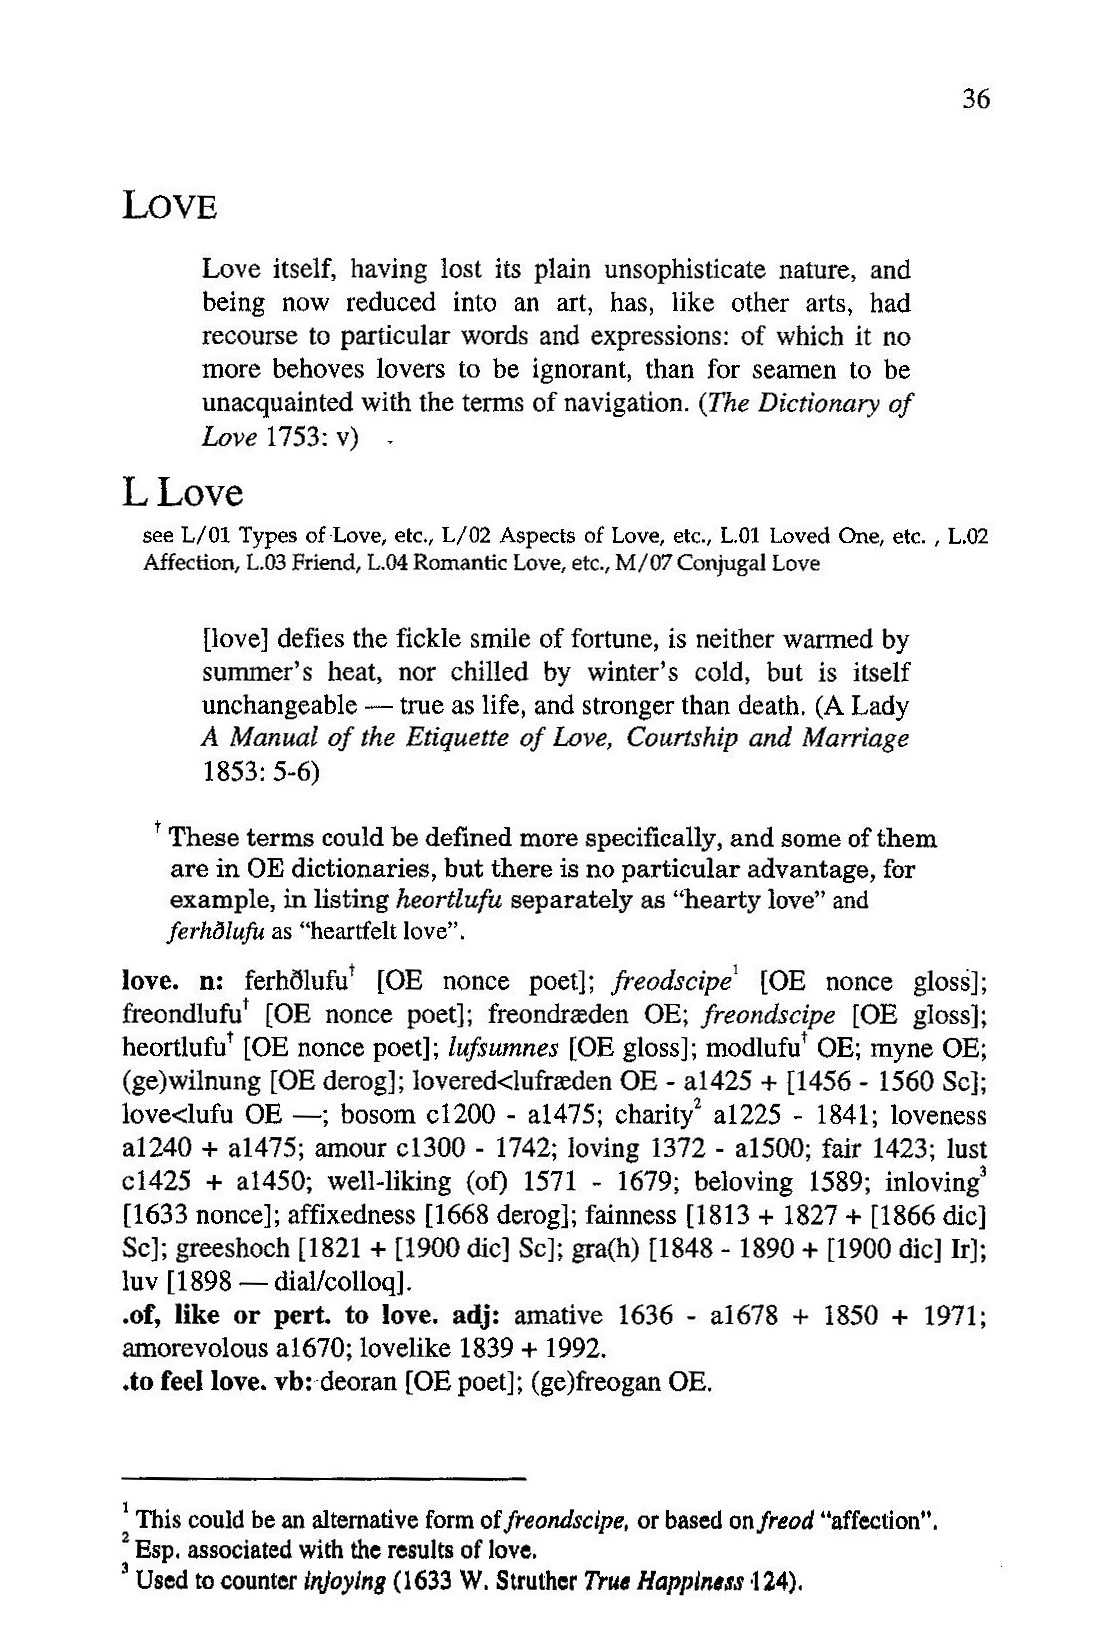
\includegraphics[width=\linewidth]{Stolk_thes-content/fig/thes/LSM-p036.jpg}
\end{minipage}%
\begin{minipage}{.5\textwidth}
  \raggedleft
  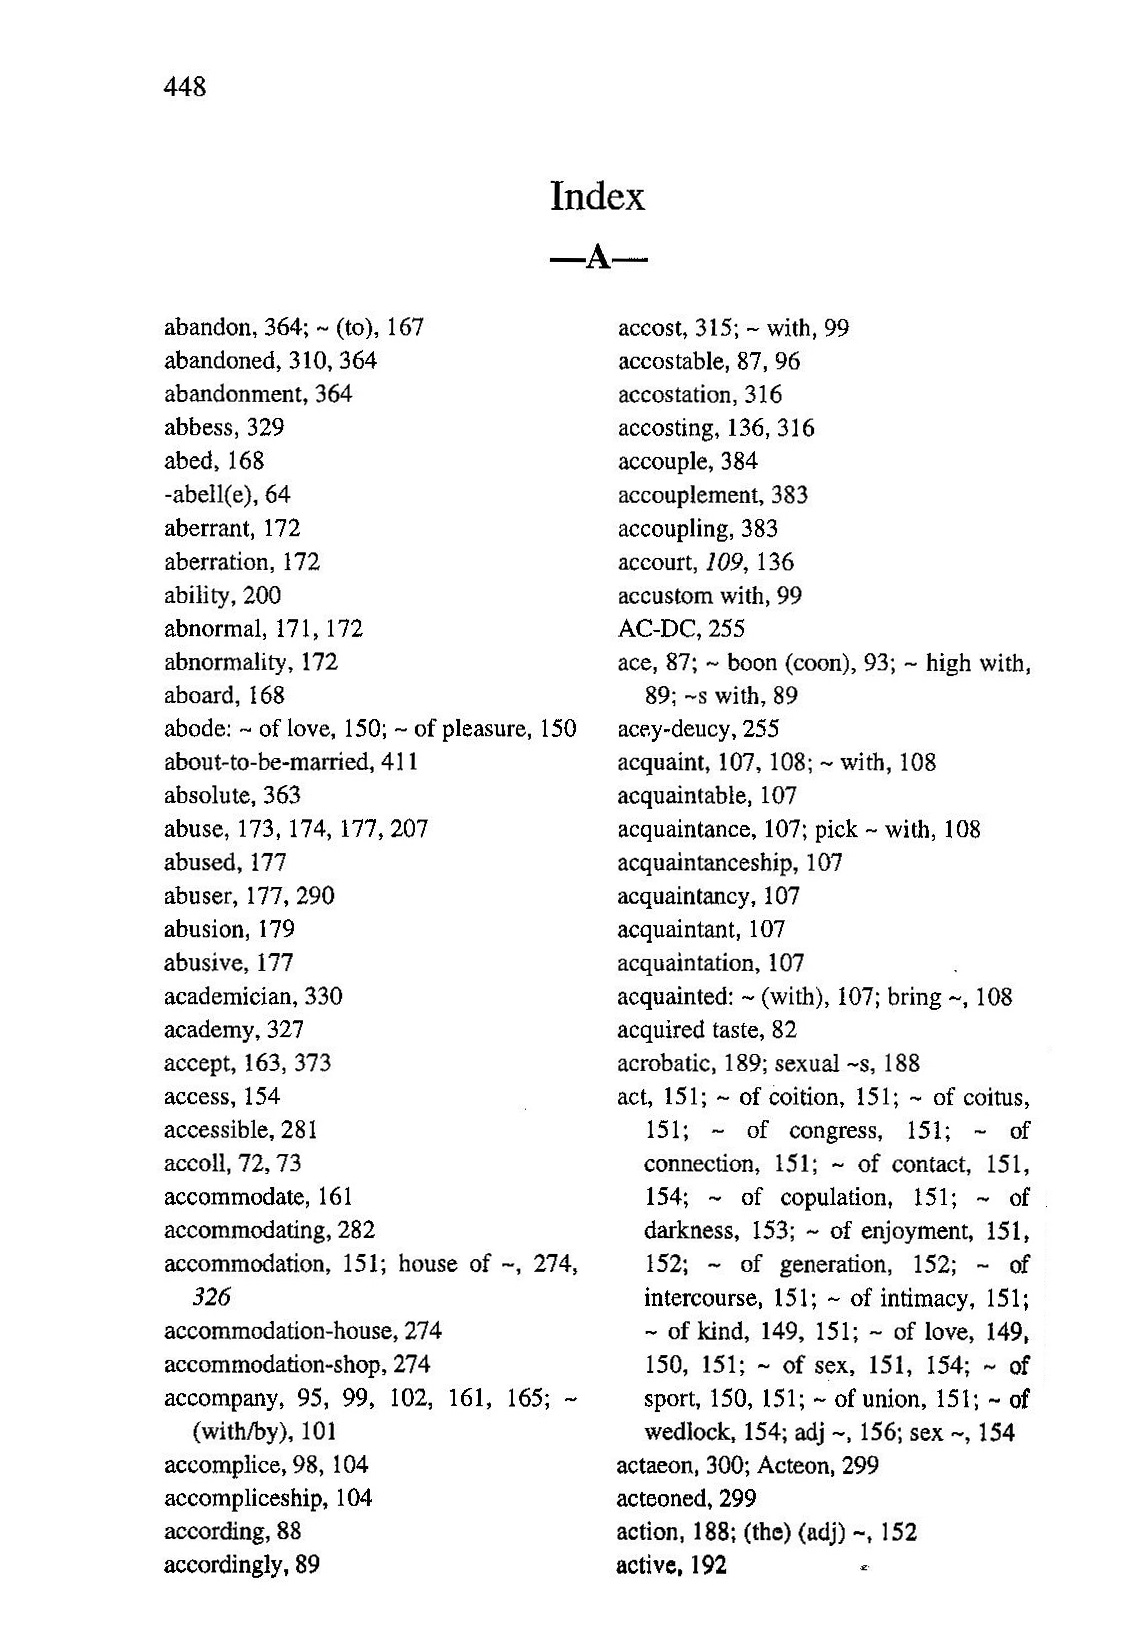
\includegraphics[width=\linewidth]{Stolk_thes-content/fig/thes/LSM-p448.jpg}
\end{minipage}
  \caption{\textit{LSM}, p. 36 and p. 448.}
  \label{fig:1.A:LSM}
\end{figure}

\noindent
\begin{figure}[htb]
  \centering
  \begin{minipage}{.5\textwidth}
    \raggedright
    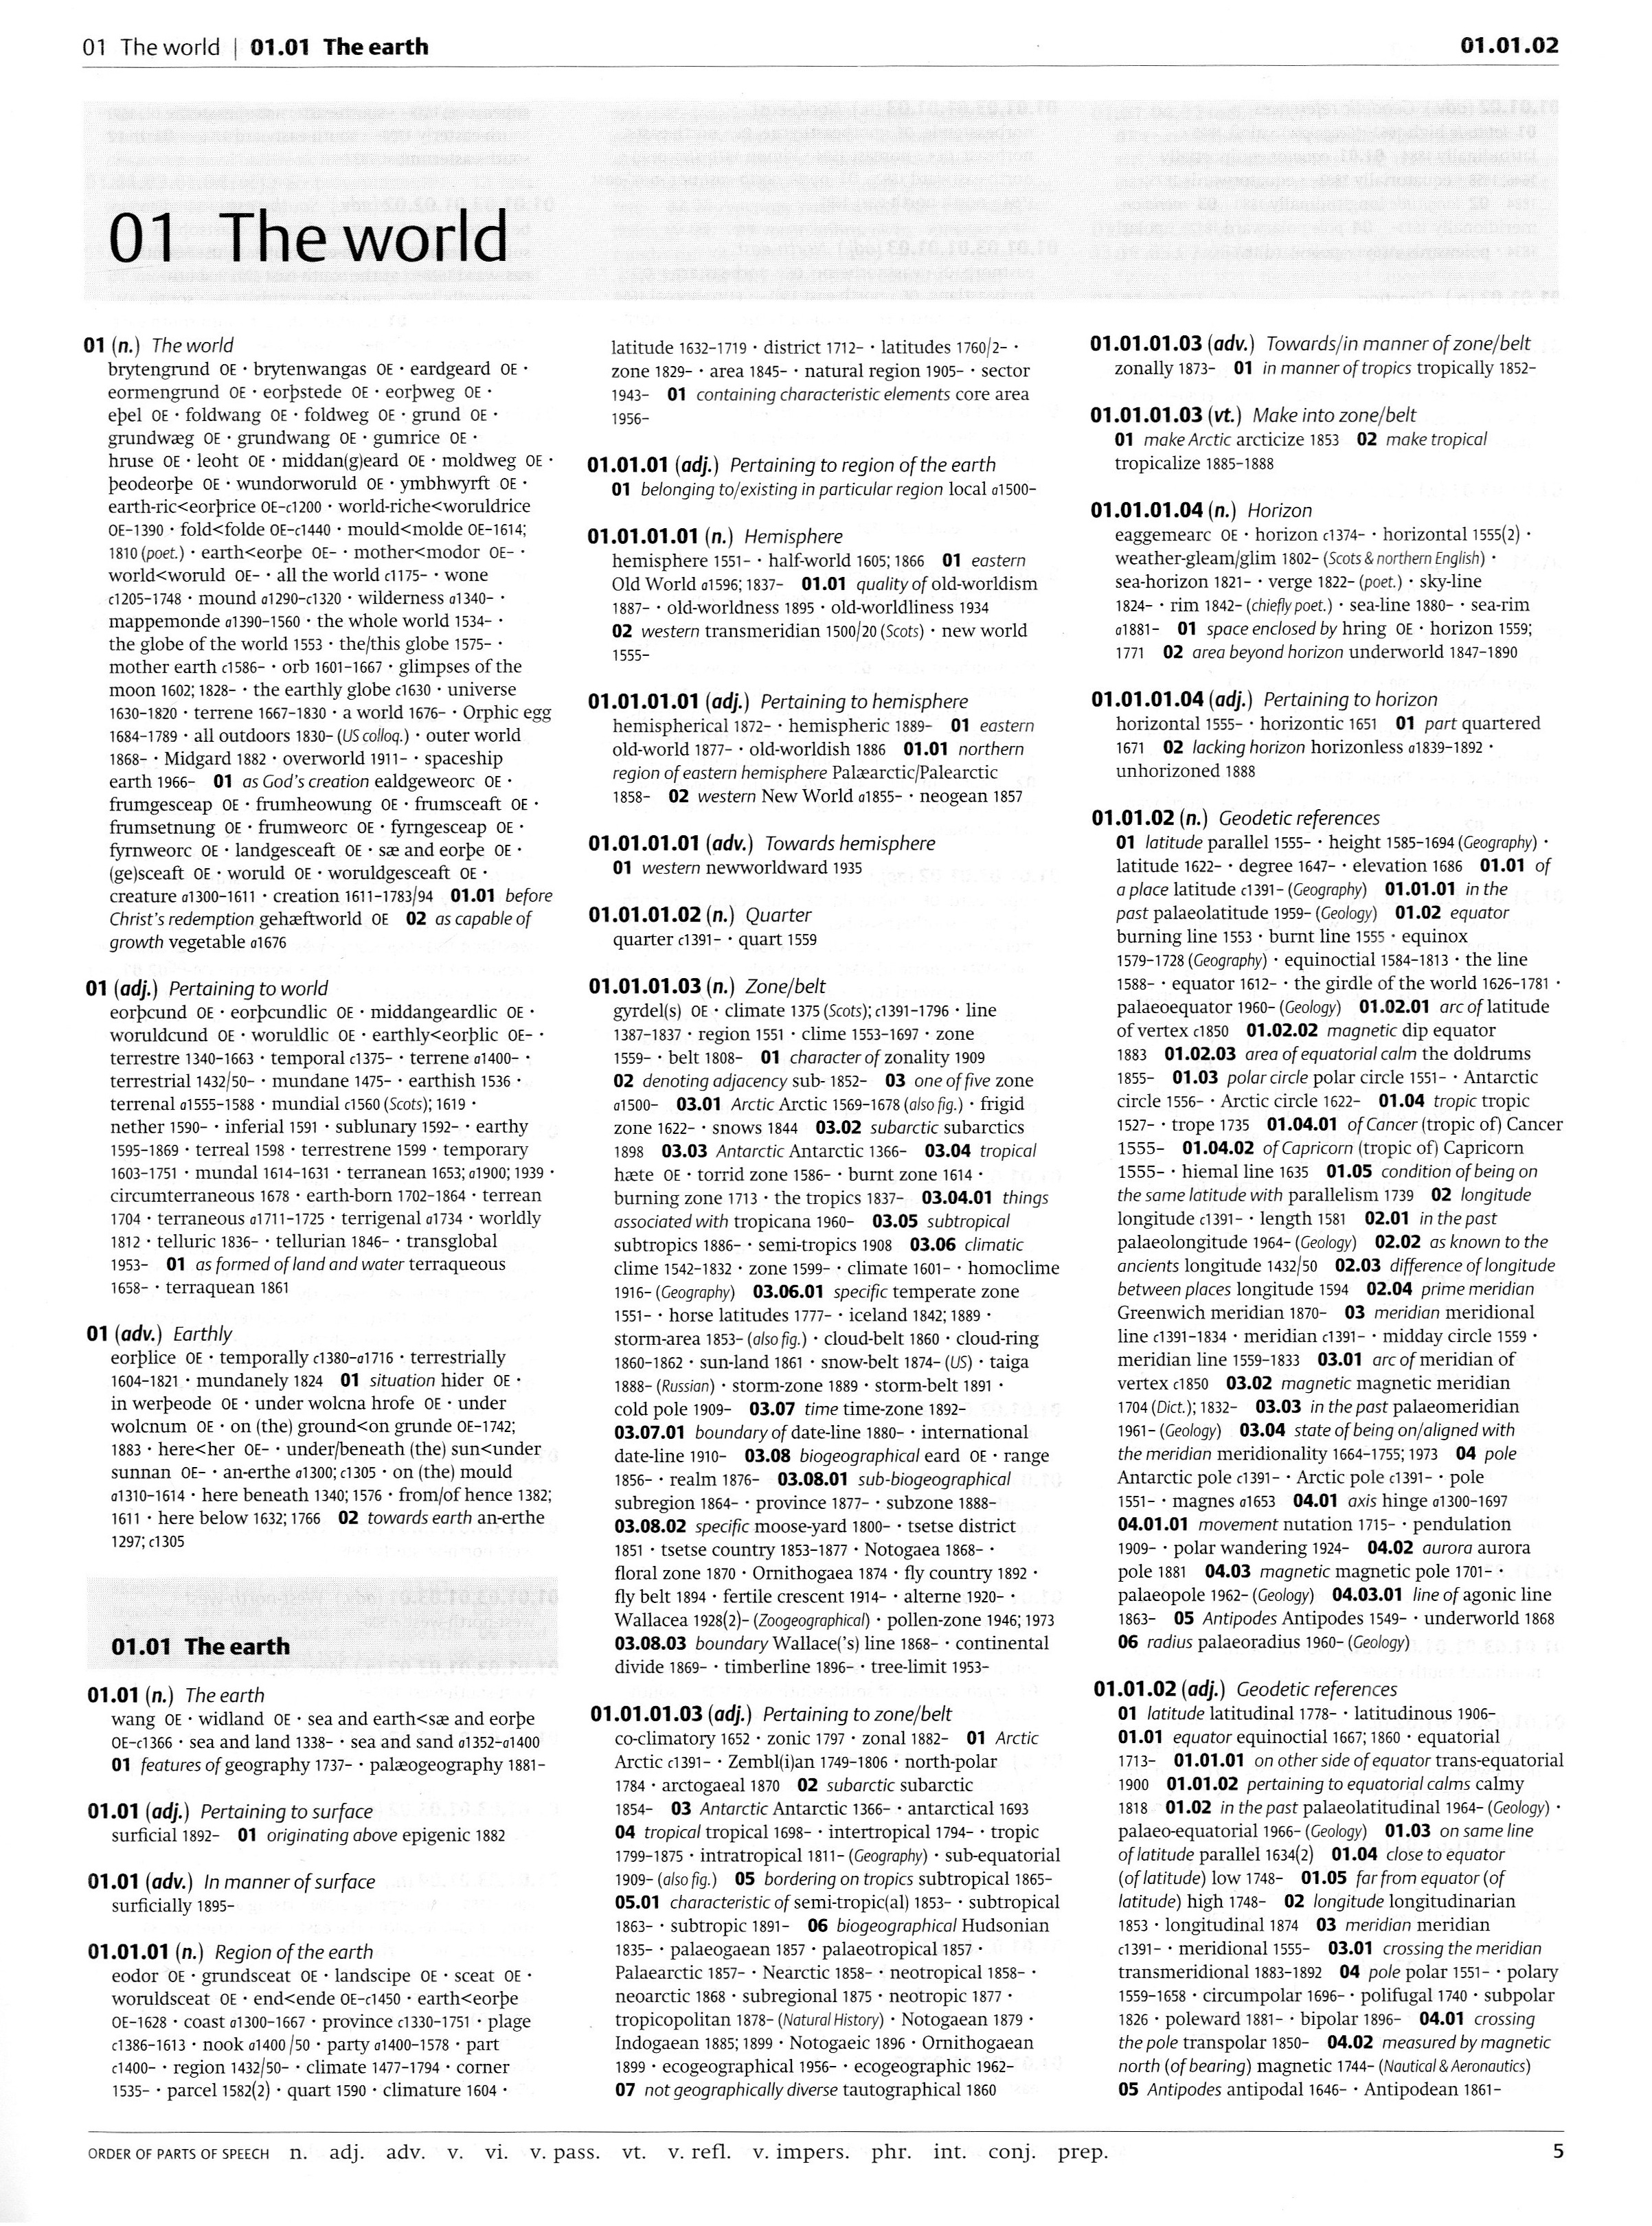
\includegraphics[width=\linewidth]{Stolk_thes-content/fig/thes/HTE1-p0005.jpg}
\end{minipage}%
\begin{minipage}{.5\textwidth}
  \raggedleft
  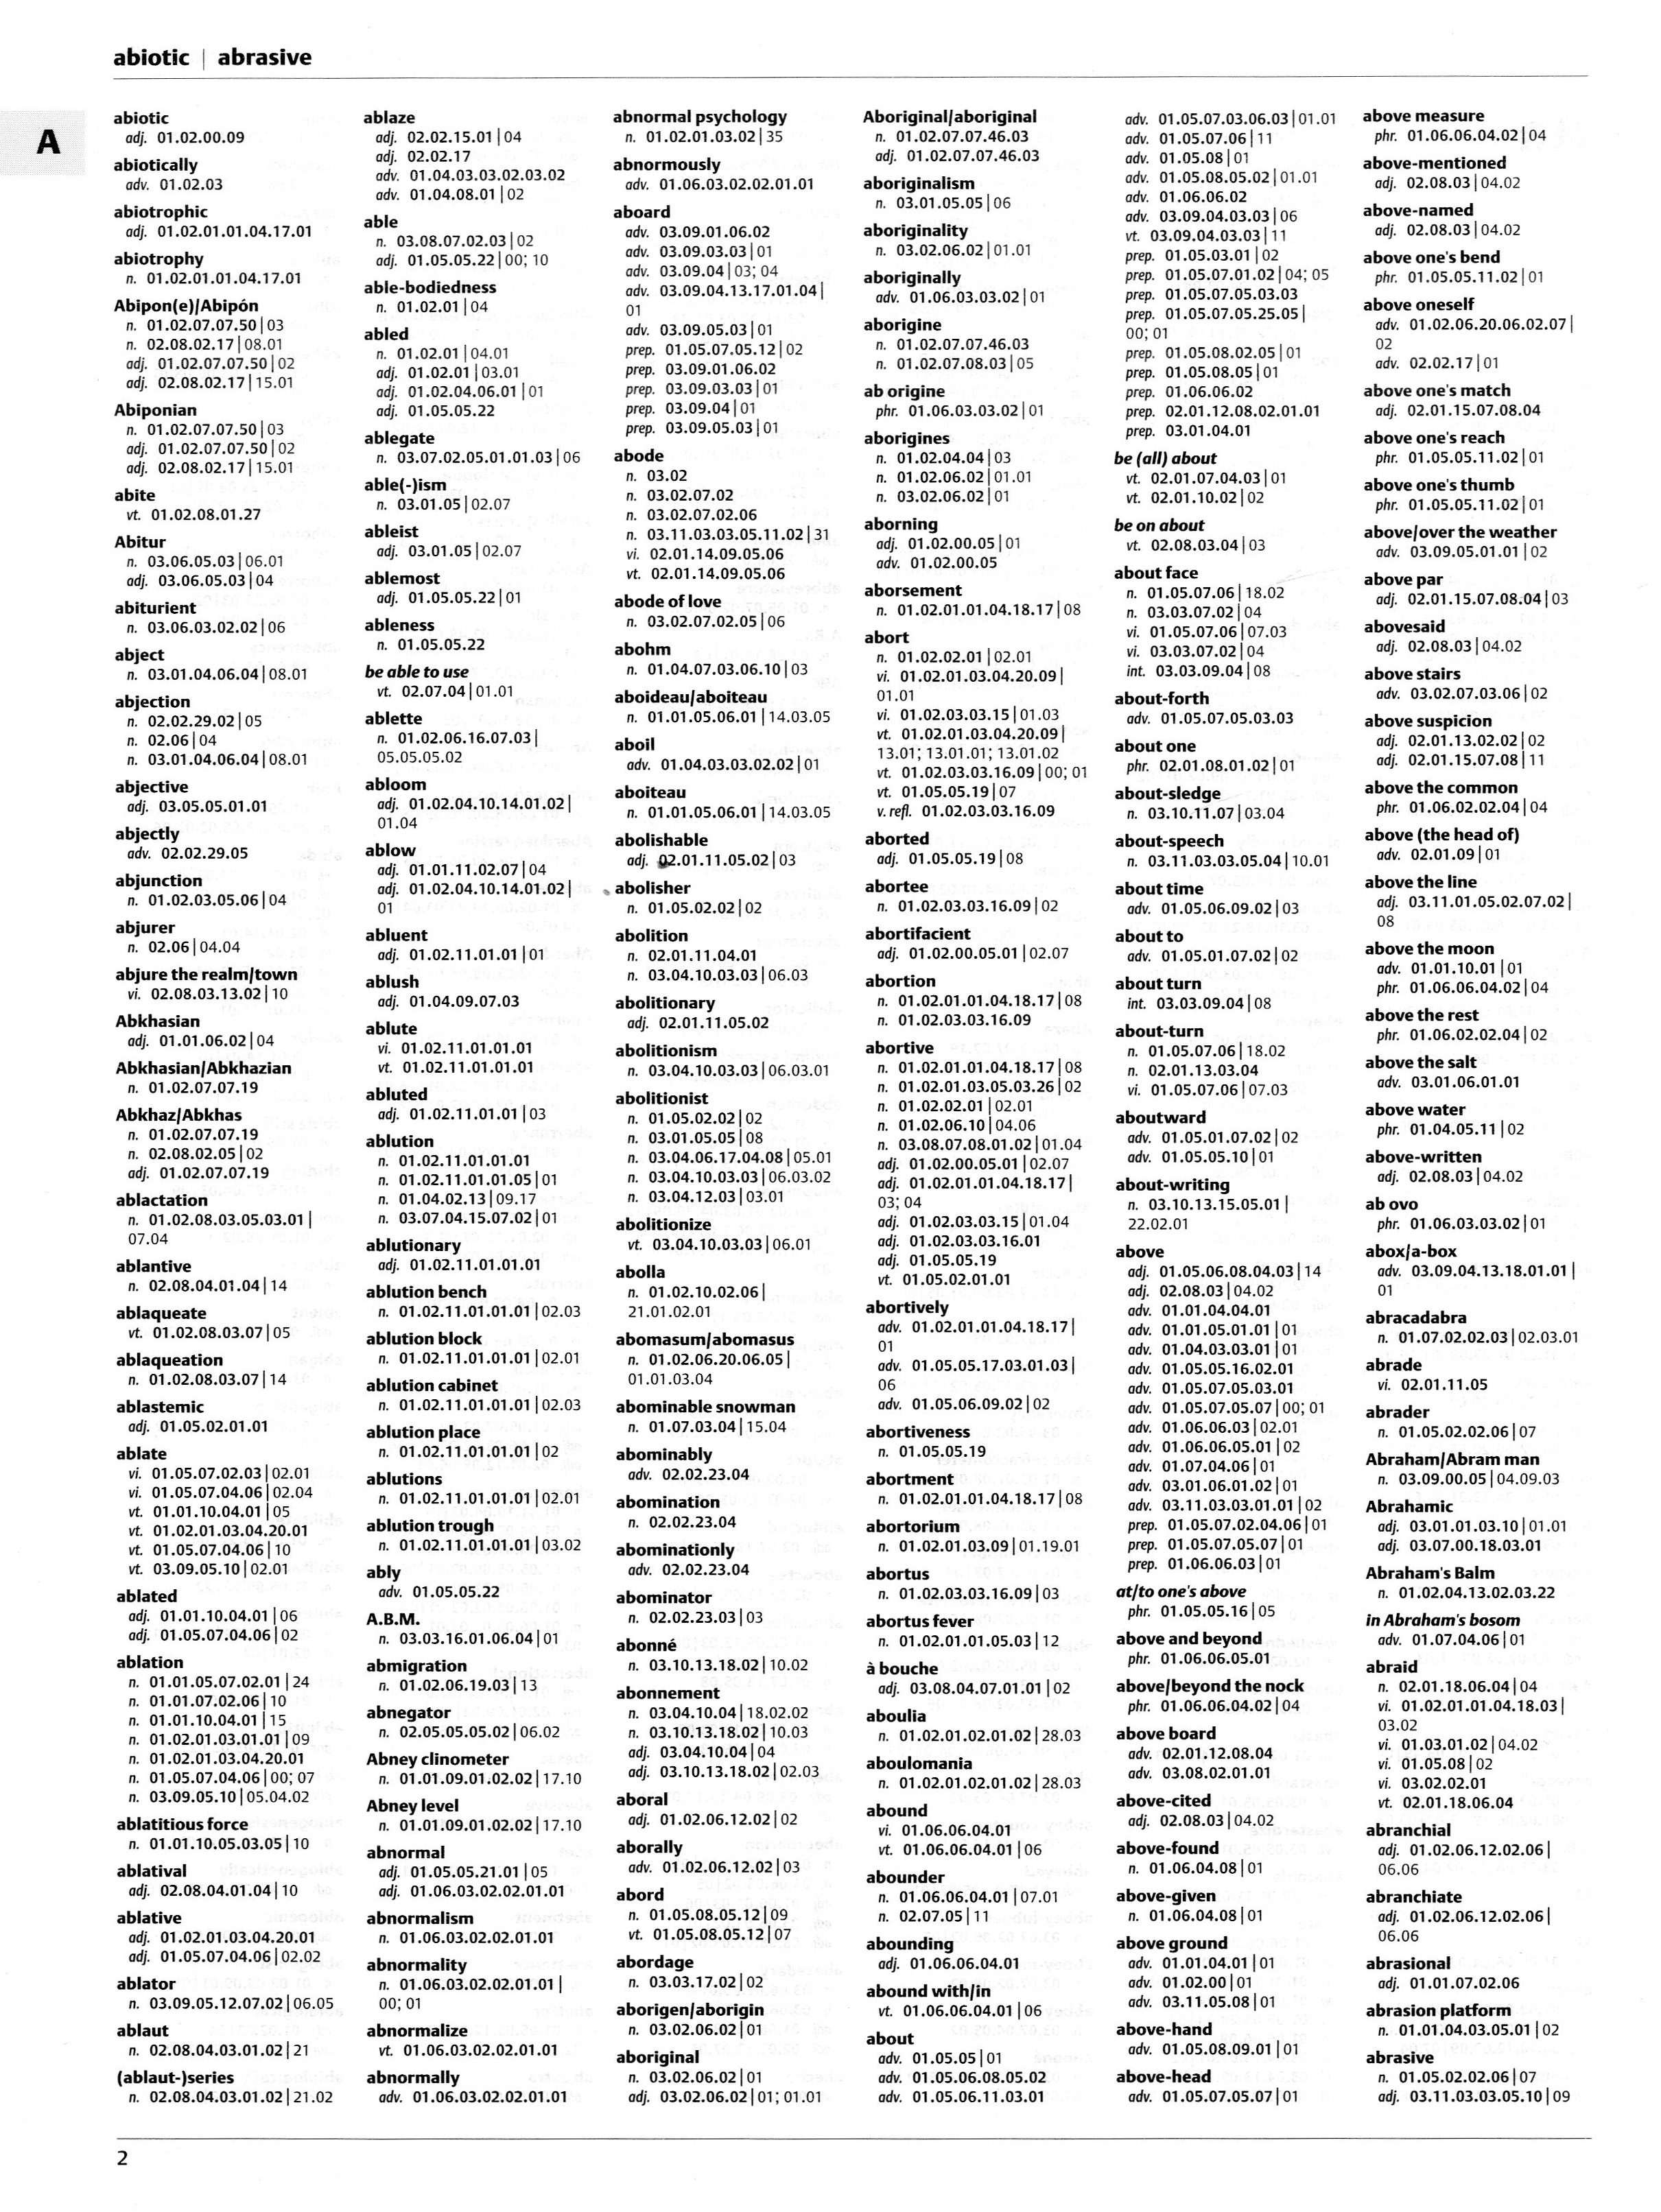
\includegraphics[width=\linewidth]{Stolk_thes-content/fig/thes/HTE1-vol2-p002.jpg}
\end{minipage}
  \caption{\textit{HTE1}, vol. 1, p. 5 and vol. 2., p. 2.}
  \label{fig:1.A:HTE1}
\end{figure}

% HTE2

% HTE3

% HTS

% BTH
\end{comment}



\endgroup



\newpage
\section*{Appendix 1.B:\\Usage features in historical language thesauri}
\label{Appendix1.B}
\begingroup
\renewcommand{\thefigure}{1.B.\arabic{figure}}
\setcounter{figure}{0}
\renewcommand{\thetable}{1.B.\arabic{table}}
\setcounter{table}{0}

This appendix details which usage features are found in the various historical language thesauri analysed in Chapter 1. First, the practice of diasystematic labelling of such features is discussed, including a typology of usage features. Afterwards, the application of each feature from this typology is considered, in separate sections, in the context of the historical language thesauri.

\subsection*{Diasystematic labelling}
\label{sect:Stolk_thes-content:diasystematic-labelling}

Usage features in thesauri and other lexicographical works tend to be conveyed through labelling, or rather diasystematic labelling. In these cases a label attached to a lexical sense is used to convey restrictions to which its use is subject.\footnote{Hartmann and James, \textit{Dictionary of Lexicography}, s.v. `diasystematic labelling'.} % (London, 1998) 
A given sense can, for instance, be labelled \textit{poetic} if it is restricted to use in poetry. Representing a label by an image or icon rather than by text (such as an anchor for nautical terms) is called iconic labelling.\footnote{Svensén, \textit{A Handbook of Lexicography}, p. 319.} 

Not only the presence of a given label may convey usage information to users --- the absence of a label may be equally meaningful. That is to say, labels are not uncommonly used to mark an element, implying that it ``deviates in a certain respect from the main bulk of items described''.\footnote{%Svensén, \textit{A Handbook of Lexicography}
Ibid., p. 315.} The absence of such a label, then, indicates that the item in question does \textit{not} deviate from this unmarked centre in terms of its usage. Thus, omitting the \textit{poetic} label for a specific sense may imply that it is found in prose. What is considered the unmarked centre and what is the periphery that is marked by labels can differ per lexicographical work.\footnote{%Svensén, \textit{A Handbook of Lexicography}
Ibid., p. 316.} 

The decisions and implications of the labelling systems in place are, according to a number of scholars, often not described with sufficient detail.\footnote{Brewer, `Labelling and Metalanguage', %in \textit{The Oxford Handbook of Lexicography}, ed. P. Durkin (Oxford, 2016), pp. 488–500 (p. 493)
p. 493.} In fact, some of the thesauri discussed here do not include a complete overview of all the labels in use and instead list the employed abbreviations only, which includes a subset of the labels found.\footnote{The thesauri that do not list all labels but only the abbreviated ones are \textit{ScT} and \textit{LSM}.} As Norri has shown, such lack of documentation is not uncommon for lexicographical works.\footnote{Norri, `Regional Labels in Some British and American Dictionaries'.} %, \textit{International Journal of Lexicography} 9.1 (1996), 1–29.
Indeed, the various editions of the \textit{OED}, too, forego of providing ``a list of status labels, or an explanation of how they are applied and what they mean''.\footnote{Brewer, `Authority and Personality in the \textit{Oxford English Dictionary}', %\textit{Transactions of the Philological Society} 103.3 (2005), 261–301 (p. 263)
p. 263.}

The labelling systems employed in dictionaries and thesauri have been subject to study, resulting in possible classifications for sets of labels that indicate a certain characteristic.\footnote{For further information on the studies and their resulting classifications, see Brewer, `Labelling and Metalanguage', p. 498.} Of these classifications, the one fashioned by Franz Josef Hausmann appears to be the most detailed.\footnote{Vrbinc and Vrbinc, `Diasystematic Information in the ``Big Five''%
', %\textit{Lexikos} 25 (2015), 424–45 (p. 426)
p. 426. See the table on pages 428–9 of their article for a clear comparison of Hausmann's classification with other existing ones. It is worth noting that the article shows that the existing classifications, including Hausmann's, are by no means exhaustive since labels, such as `figurative' and `trademark', are not yet covered by them (p. 429).} This classification provides a clear and useful framework that will be employed in this section to discuss the usage feature information found in the historical language thesauri.\footnote{Hausmann, `Die Markierung im allgemeinen einsprachigen Wörterbuch%: eine Übersicht
', %in \textit{Wörterbücher: Ein internationales Handbuch zur Lexikographie}, eds. F. J. Hausmann et al. (Berlin, 1989), vol.1, pp. 649–57 (pp. 651–2)
pp. 651-2.} Table \ref{table:Stolk_thes-content:diasystematic-marking} below presents an overview of Hausmann's typology in the context of a contemporary general-purpose dictionary. 

\begin{table}[h!]
    \centering
    \small
    { \RaggedRight
    \begin{tabular}{p{0.05in}lp{0.8in}p{0.8in}p{0.75in}p{0.95in}}
    \toprule
        & \textbf{Criterion} & \textbf{Type of marking} & \textbf{Unmarked centre} & \textbf{Marked periphery} & \textbf{Examples of labels} \\
    \midrule
1 & 
Time & 
diachronic & 
contemporary language & 
archaism--neologism & 
\textit{arch.}, \textit{dated}, \textit{old use} \\ \hline
2 &
Place &
diatopic &
standard language &
regionalism, dialect word &
\textit{AmE}, \textit{Scot.}, \textit{dial.} \\ \hline
3 &
Nationality &
diaintegrative &
native word &
foreign word &
\textit{Lat.}, \textit{Fr.} \\ \hline
4 &
Medium &
diamedial &
neutral &
spoken--written &
\textit{colloq.}, \textit{spoken} \\ \hline
5 &
Socio-cultural &
diastratic &
neutral &
sociolects &
\textit{pop.}, \textit{slang}, \textit{vulgar} \\ \hline
6 &
Formality &
diaphasic &
neutral &
formal--informal &
\textit{fml}, \textit{infml} \\ \hline
7 &
Text type &
diatextual &
neutral &
poetic, literary, journalese &
\textit{poet.}, \textit{lit.} \\ \hline
8 &
Technicality &
diatechnical &
general language &
technical language &
\textit{Geogr.}, \textit{Mil.}, \textit{Biol.}, \textit{Mus.} \\ \hline
9 &
Frequency &
diafrequential &
common &
rare &
\textit{rare},\newline \textit{occas.} \\ \hline
10 &
Attitude &
diaevaluative &
neutral &
connoted &
\textit{derog.}, \textit{iron}., \textit{euphem.} \\  \hline
11 &
Normativity &
dianormative &
correct &
incorrect &
\textit{non-standard} \\
    \midrule
    \end{tabular}
    }
    \caption[]{\label{table:Stolk_thes-content:diasystematic-marking}Diasystematic marking in a contemporary general-purpose dictionary.\protect\footnotemark}
\end{table}
\footnotetext{Reproduced from Svensén, \textit{A Handbook of Lexicography}, p. 316.}

As Table \ref{table:Stolk_thes-content:diasystematic-marking} shows, the periphery indicated by labels used in a particular type of marking may be based on a scale (e.g., ranging from archaism to neologism, or from formal to informal). Markings based on such a scale may not be limited to just those covering diachronic, diamedial, and diaphasic usage features.\footnote{Hartmann and James, \textit{Dictionary of Lexicography}, s.v. `diaevaluative information', `diafrequential information', `diaintegrative information', `dianormative information', `diastratic information', `diatextual information', and `diatopical information'.} Another relation between labels may also exist, as pointed out by Atkins and Rundell. Diatechnical labels, for instance, may well be positioned in a hierarchical structure.\footnote{Atkins and Rundell, \textit{The Oxford Guide to Practical Lexicography}, pp. 184.} The labels `Biology' and `Astronomy', for example, could be subordinate to the more general `Science'. Such a hierarchy has two benefits for editors: it makes it easier to ensure that no required labels are omitted and allows for more accurate (but also coarser) marking of items.\footnote{Ibid.}%Atkins and Rundell, \textit{The Oxford Guide to Practical Lexicography}, pp. 184.


Although Hausmann's typology was suggested within the subject of marking, it is useful in the broader context of lexicographical information on usage as well. Its criteria and types of marking identified can be applied to such information, regardless of whether labels are employed and regardless of whether an unmarked centre exists. Table \ref{table:Stolk_thes-content:HLT-usage-info} provides an overview of which kinds of usage information are conveyed systematically in the historical language thesauri analysed.


\begin{table}[h!]
    \centering
    \small
    { \setlength{\tabcolsep}{0.08in}
    \begin{tabular}{lcccccccc}
    \toprule
        % TODO: REORDER COLUMNS & VALUES TO THESAURUS ORDER USED IN INTRO
%        &
%        \textbf{Criterion} &
        \textbf{Type} &
        \textbf{\textit{TOE}} &
        \textbf{\textit{HTE}} &
        \textbf{\textit{BTH}} &
        \textbf{\textit{ShT}} &
        \textbf{\textit{ScT}} &
        \textbf{\textit{HTS}} &
        \textbf{\textit{LSM}} &
        \textbf{\textit{DSSPIEL}} \\
    \midrule
%1 &
%Time &
Diachronic &

- &
+ &
+ &
- &
+ &
- &
+ &
- \\

%2 &
%Place &
Diatopic &

- &
+ &
- &
- &
+ &
- &
+ &
- \\
%3 &
%Nationality &
Diaintegrative &

- &
+ &
- &
- &
- &
- &
+ &
- \\
%4 &
%Medium &
Diamedial &

- &
+ &
- &
- &
+ &
- &
+ &
- \\
%5 &
%Socio-cultural &
Diastratic &

- &
+ &
- &
- &
+ &
- &
+ &
- \\
%6 &
%Formality &
Diaphasic &

- &
~~~~~- \protect\footnotemark &
- &
- &
+ &
- &
- &
- \\
%7 &
%Text type &
Diatextual &

+ &
+ &
- &
- &
+ &
- &
+ &
- \\
% &
%Technicality &
Diatechnical &

- &
+ &
- &
- &
+ &
- &
+ &
- \\
%9 &
%Frequency &
Diafrequential &

+ &
+ &
- &
- &
+ &
- &
+ &
- \\
%10 &
%Attitude &
Diaevaluative &

- &
+ &
- &
- &
+ &
- &
+ &
- \\
%11 &
%Normativity &
Dianormative &

+ &
+ &
- &
- &
- &
- &
+ &
- \\
    \midrule
    \end{tabular}
    }
    \caption[]{\label{table:Stolk_thes-content:HLT-usage-info}Overview of usage information present in historical language thesauri.}
\end{table}
\footnotetext{Diaphasic information, at least in terms of `formal' and `informal' labels, is not present in \textit{HTE3} apart from what can only be perceived as a stray marking of a single sense as `formal': \textit{ponor} in category ``01.01.04.04.02.02|11 Land :: Hole/pit :: pot-hole/swallow-hole''.} 



As the overview in Table \ref{table:Stolk_thes-content:HLT-usage-info} shows, many different kinds of usage features are systematically incorporated into historical language thesauri. 
%A more in-depth discussion on the application of these usage features is available in Appendix 1.B. 
Most features are indicated through systematic labelling. What a label indicates can differ from one thesaurus to another. A case in point is the `poetic' label, which in some thesauri signals that a word has a poetic flavour (e.g., \textit{HTE}) but in others that a word is found solely in poetic works (e.g., \textit{TOE}). Moreover, a label may encompass a greater or smaller range (e.g., for what is still considered `formal' or `informal') or even mark word forms or lexemes rather than senses (such as with the distribution flags found in \textit{TOE}).\footnote{Atkins and Rundell, \textit{The Oxford Guide to Practical Lexicography}, pp. 182–6.} A label should therefore always be seen within the defined context of its body, be it a dictionary or thesaurus, and may or may not overlap with use of that same label in a different body. %Users of a thesaurus would benefit from access to a guide on the various labels that it employs. Understanding of these labels may be enhanced by having the guide discuss labels together that are based on the same type of usage feature and by informing the user of how these labels based on the same criterion are related exactly.

Labels based on the same criterion can be related in a number of ways. Some are based on a scale; others can be positioned in a hierarchy. More intricate relations exist as well, as evidenced by diatopic usage features. The regions indicated by diatopic labels may be related to each other in various ways.\footnote{Randell et al., `A Spatial Logic Based on Regions and Connection'.} %, in \textit{Proc. 3rd Int. Conf. on Knowledge Representation and Reasoning} (San Mateo, 1992).
One region may, for example, contain, touch, or overlap with another. The regions indicated by labels are presented most vividly by a map, as is done in \textit{ScT}, which allows the user to deduce the spatial relations between them.\footnote{\textit{ScT}, pp. xvii-xviii.}

%Usage features can also be conveyed through means other than labels. Diachronic usage features, for instance, are captured in \textit{LSM} and \textit{HTE} through dates of currency. The methods employed in both thesauri to present these dates can be somewhat complex, partly due to the need to represent levels of certainty for dates provided.\footnote{\textit{LSM}, pp. 28–9; \textit{HTE}, pp. xxii–xxiii.} %In short, spatio-temporal usage features may require special attention once these need to be captured, presented, and queried in a digital environment.


\subsection*{Diachronic information}
\begin{quotation} \noindent
A usage feature which associates a word or phrase with a particular PERIOD in the history of a language. Such information can be marked in dictionaries by temporal USAGE LABELS on a chronological scale from `archaic' through `obsolescent' to contemporary (the unmarked neutral, synchronic zone) and `new'.\footnote{Hartmann and James, \textit{Dictionary of Lexicography}, s.v. `diachronic information'.}
\end{quotation}
The currency of lexical senses are known in historical language thesauri. The senses found in \textit{TOE}, for instance, belong to the Old English lexis, spoken between roughly 500 and 1100 A.D. by the Anglo-Saxons. Explicit diachronic information that further subdivides the period treated is not available in every historical language thesaurus. In fact, \textit{TOE} treats its items as ``a single geographically and temporally indistinguishable mass'', ignoring diachronic differences between, e.g., Early West Saxon and Late West Saxon.\footnote{Dance, Review of \textit{TOE1}, p. 313.} 
% reference used to be here in full as: R. Dance, Review of \textit{TOE1}, \textit{Medium Ævum} 66.2 (1997), 312-13 (p. 313).
The currency of senses, then, is left implicit to be either within or overlap with the period specific to the thesaurus. Such a lack of explicit, finer-grained diachronic information on the currency of senses also holds true for \textit{HTS} (or at least, for the pilot version available at the time of writing), \textit{ShT}, and \textit{DSSPIEL}.

Some of the historical language thesauri carry a finer-grained indication of the currency of their lexical items. \textit{ScT} labels its senses as obsolete (with †) for cases where, as its editor states, ``we have no evidence [for their use] in the twentieth century''.\footnote{\textit{ScT}, p. xv.} This system divides the currency of lexical senses effectively into two periods: those in use only before the twentieth century and those used also after the turn of that century. A yet greater distinction on currency than the aforementioned, relatively crude, labelling categorisation employed by \textit{ScT} is present in \textit{HTE}. Each lexical sense in this thesaurus ``is accompanied by its dates of recorded use''.\footnote{\textit{HTE1}, p. ix.} This information allows users to focus on the English vocabulary available in a specific time frame, such as that available to Shakespeare.\footnote{%\textit{HTE1}
\textit{HTE1}, p. xiv.} \textit{LSM} and \textit{BTH}, too provide such citation dates for the currency of their items. %The latter largely drawing on the information on slips that was also used to form \textit{HTE}.

\subsection*{Diatopic information}
\begin{quotation} \noindent
A usage feature which associates a word or phrase with a particular DIALECT or regional language variety. Such features can be marked in dictionaries by USAGE LABELS on a continuum of regionality from `local' or `provincial' dialects to `metropolitan' and even `international' varieties. The neutral zone of the `home' variety (e.g. British English in a British dictionary or American English in an American dictionary) may be left unmarked.\footnote{Hartmann and James, \textit{Dictionary of Lexicography}, s.v. `diatopic(al) information'.}
\end{quotation}
Three of the historical language thesauri contain diatopic information: \textit{ScT}, \textit{HTE}, and \textit{LSM}. Each of these contain the label `dialectal' (abbreviated to `dial' or `dial.').\footnote{Abbreviations, including those of labels, can be found on p. xxxi of \textit{HTE1} and pp. 33-5 of \textit{LSM}.} Next to this particular marking of dialectal items, these three thesauri may also attribute a specific region to lexical senses through labels. \textit{HTE} and \textit{LSM} share a number of such regional labels, including Australian (abbreviated to `Aus' or `Austral'), New Zealand (`NZ'), and United States (`US'). \textit{ScT}, focused on the Scottish vocabulary, contains senses that are not as widely dispersed in use as those in \textit{HTE} and \textit{LSM}. Its diatopic information is, perhaps for that very reason, more specialized in nature and conveys a number of levels of granularity. The main dialect divisions which this thesaurus distinguishes for the Scottish lexis are Northern, North-East, Central, and Southern Scots, with a subdivision of Central Scots into East Central, West Central, and South-West Scots.\footnote{\textit{ScT}, p. xvii.} More precise regional distinctions are provided by labels representing pre-1975 counties, such as Shetland, Aberdeen, Edinburgh, and Selkirk.\footnote{%\textit{ScT}
\textit{ScT}, p. xv.} These regional divisions are clarified visually through maps.\footnote{%\textit{ScT}
\textit{ScT}, p. xvii.} In short, the diatopic information in the thesauri is provided by labels indicating regions --- regions that may themselves be subdivided into smaller identifiable regions for increased specificity.

\subsection*{Diaintegrative information}
\begin{quotation} \noindent
A usage feature which associates a word or phrase with a particular degree of integration into the native word-stock of the language. Such information can be marked in dictionaries by USAGE LABELS on a scale of indigenisation ranging from `foreign' and `borrowed' through `assimilated' to native (the unmarked neutral zone).\footnote{Hartmann and James, \textit{Dictionary of Lexicography}, s.v. `diaintegrative information'.}
\end{quotation}
Two of the historical language thesauri contain diaintegrative information: \textit{LSM} and \textit{HTE}. These thesauri mark senses of lexemes that have been borrowed from other languages and are not yet considered assimilated or native. To illustrate, both thesauri label \textit{shadchan} as `Jewish' and \textit{nakodo} as `Japanese', each in the sense of ``one who makes matches''. Unfortunately, the labels appear to be used rather inconsistently. Thus, \textit{HTE} labels \textit{kamikaze} as `Japanese' for some senses, but not for others. In \textit{LSM}, \textit{maîtresse en titre} is not labelled as French but instead as `unnaturalized' (abbreviated as `unnat') --- a label seemingly just as suitable for, but not applied to, \textit{shadchan} and \textit{nakodo}.

In a multilingual thesaurus, language labels tend not to convey diaintegrative information but the language of its words and phrases (cf. \textit{DSSPIEL} and \textit{BTH}). The distinguishing factor between the two uses of these labels -- i.e., diaintegrative usage versus language -- is whether a lexical item is used solely in the context of a certain language or used within another language context. That is to say, if a word is employed frequently enough in a native rather than a foreign context, then the loan word may be considered part of the native lexis, albeit perhaps with its foreign origins still recognisable. Monolingual lexicographical works will, by their very definition, consider only a single language and therefore adopt these labels to portray diaintegrative usage information.

\subsection*{Diamedial information}
\begin{quotation} \noindent
A usage feature which associates a word or phrase with a particular channel of communication. Such information can be marked in some dictionaries by USAGE LABELS for the `written' or `spoken' media, while items shared by both are usually left unmarked.\footnote{%Hartmann and James, \textit{Dictionary of Lexicography}
Ibid., s.v. `diamedial information'.}
\end{quotation}
Although none of the thesauri treated here employ the labels `written' and `spoken', a number of them do mark lexical senses with another diamedial label: `colloquial'. This label is employed by \textit{ScT}, \textit{HTE}, and \textit{LSM} (abbreviated to `colloq') for terms used in daily speech.

\subsection*{Diastratic information}
\begin{quotation} \noindent
A usage feature which associates a word or phrase with a particular social group. Such information can be marked in dictionaries by USAGE LABELS on a scale from neutral (the unmarked zone) to `demotic' or `slang'. In some cultures, such as the Indian caste system, there may be an extension of the scale towards the `high' varieties. There is often an overlap with DIAPHASIC INFORMATION.\footnote{%Hartmann and James, \textit{Dictionary of Lexicography}
Ibid., s.v. `diastratic information'.}
\end{quotation}
Three of the historical language thesauri contain diastratic information: \textit{LSM}, \textit{HTE}, and \textit{ScT}.\footnote{Although the use of the label `slang' is not indicated in the introduction of \textit{ScT}, it is certainly employed systematically as evidenced by the lexical sense of \textit{bung} in category ``2.4 Horses, donkeys''.} All of these contain the label `slang' (abbreviated in \textit{LSM} to `sl'). \textit{HTE} describes the meaning of this label as one denoting ``very informal language that is often restricted to a particular social group''.\footnote{\textit{HTE1}, p. xxiv.} Labels indicating a specific form of slang, namely rhyming slang, are found in \textit{LSM} (where it is abbreviated to `Rsl'). One instance for which this label is applied is the phrase \textit{trouble and strife} in the sense of wife.\footnote{See \textit{LSM} category ``M.01.01.01 Wife''.} In addition to `slang', both \textit{LSM} and \textit{HTE} employ the diastratic label `vulgar' (abbreviated to `vulg' in \textit{LSM}) for lexical senses that are considered rude or obscene.\footnote{\textit{LSM}, p. 35; \textit{HTE1}, p. xxiv.}

\subsection*{Diaphasic information}
\begin{quotation} \noindent
A usage feature which associates a word or phrase with a particular REGISTER of a language. Such information can be marked in dictionaries by USAGE LABELS on a scale from `elevated' and `formal' through neutral (the unmarked zone) to `informal' and `intimate'. There is often an overlap with DIASTRATIC INFORMATION.\footnote{Hartmann and James, \textit{Dictionary of Lexicography}, s.v. `diaphasic information'.}
\end{quotation}
Diaphasic information is conveyed in \textit{ScT} through the label `informal'.\footnote{The marking `informal' in \textit{ScT} is, for instance, attributed to \textit{Royal} in category ``12.2 Soldiers and other services personnel''.} \textit{HTE} makes no mention of that specific label in its front matter, but contains what appears to be a single stray application of the label `formal'.\footnote{The marking `formal' in \textit{HTE3} can be found for the lexical sense \textit{ponor} in category ``01.01.04.04.02.02|11. pot-hole/swallow-hole''.} Diaphasic markings do not seem to be present in the other thesauri analysed in the chapter.

\subsection*{Diatextual information}
\begin{quotation} \noindent
A usage feature which associates a word or phrase with a particular discourse type or GENRE. Such information can be marked in dictionaries by USAGE LABELS on a scale of textuality from `poetic' to `conversational', with the shared neutral items remaining unmarked. There is often an overlap or combination with DIAPHASIC and DIASTRATIC information.\footnote{Hartmann and James, \textit{Dictionary of Lexicography}, s.v. `diatextual information'.}
\end{quotation}
The historical language thesauri analysed that employ usage labels all include diatextual information. One example is the restricted use to poetry or verse, which is indicated by a label in \textit{TOE} (with the \textit{p}-flag), \textit{HTE} and \textit{LSM} (with the abbreviated label `poet') as well as \textit{ScT} (using the label `verse'). A second example is the label for glossaries that is applied in \textit{TOE} (with the \textit{g}-flag) and \textit{LSM} (with the abbreviation `gloss'). However, as the editor of \textit{LSM} notes, identical diatextual labels found in different thesauri may not have the same meaning that they have at first glance: contrary to the practice in \textit{LSM}, the editors of \textit{TOE} employ the glossary label to ``flag terms occurring only in glossaries, but not terms found in glosses''.\footnote{\textit{LSM}, p. 34.} Moreover, the labels in \textit{TOE} ``relate only to word forms, not to meaning''.\footnote{\textit{TOE2}, p. xxi.} In other words, even though they may be presented at every lexical sense, these labels do not indicate usage features of each sense separately. The editors of \textit{TOE} state that such labelling per sense will demand further efforts in Old English lexicography.\footnote{textit{TOE2}, p. xxii.}

\subsection*{Diatechnical information}
\begin{quotation} \noindent
A usage feature which associates a word or phrase with a particular SUBJECT FIELD. Such information can be marked in dictionaries by USAGE LABELS for a range of technical specialities, e.g. `Law', `Music', `Chemistry'. The CORE WORDS common to non-technical language varieties are usually left unmarked, as is non-specific, `vague' vocabulary.\footnote{Hartmann and James, \textit{Dictionary of Lexicography}, s.v. `diatechnical information'.}
\end{quotation}
\textit{ScT} contains at least one label referring to a subject field: archaeology.\footnote{This label is never found as `archeol', the abbreviation listed in the introduction, but rather as `archaeol'. See, for instance, \textit{yett} in category ``13.3.5 Castles etc.''.} \textit{HTE} and \textit{LSM} both contain several diatechnical labels, a number of which are shared; both draw from the \textit{OED}, which includes such markings, as their source. Subject fields indicated by labels in the two thesauri include archaeology, nautical, military, theatre, and botany.

\subsection*{Diafrequential information}
\begin{quotation} \noindent
A usage feature which associates a word or phrase with a particular FREQUENCY of occurrence. Such information can be marked in dictionaries by USAGE LABELS ranging from `very frequent' to frequent (the unmarked neutral zone) to `becoming rare' and `very rare'.\footnote{Hartmann and James, \textit{Dictionary of Lexicography}, s.v. `diafrequential information'.}
\end{quotation}
Four of the historical language thesauri treated here annotate their lexical senses with diafrequential information. Three of them -- \textit{ScT}, \textit{LSM}, and \textit{HTE} -- mark senses when they are rare. Extremely rare items, or nonce words, are marked in \textit{TOE}, \textit{LSM}, and \textit{HTE}. Such items occur only once in the corpus that the thesaurus (directly or indirectly) is based on. \textit{TOE} employs the \textit{o}-flag for this marking; \textit{LSM} and \textit{HTE} use the label `nonce' and `nonce word' respectively.\footnote{\textit{TOE2}, pp. xxi–xxv; \textit{LSM}, p. 34; \textit{HTE1}, p. xxiv.} The editors of these works are aware that designating a word form in a specific sense as a nonce word, or \textit{hapax legomenon}, is fraught with problems.\footnote{\textit{TOE2}, p. xxi.} Do derivations of the word found in another part of speech negate the status of nonce? Does evidence in a later phase of the language than that treated in the thesaurus entail that a word should not be marked as nonce? If the corpus is expanded, is it not likely that the nonce status may disappear? As the editors of \textit{TOE} state, such labelling of nonce words ``as often as not should serve to give rise to speculation and inquiry''.\footnote{\textit{TOE2}, p. xxv.}

\subsection*{Diaevaluative information}
\begin{quotation} \noindent
A usage feature which associates a word or phrase with a particular attitude or evaluation. Such information can be marked in dictionaries by USAGE LABELS on a scale of emotiveness from `appreciative' through neutral (the unmarked zone) to `derogatory' and `offensive'.\footnote{Hartmann and James, \textit{Dictionary of Lexicography}, s.v. `diaevaluative information'.}
\end{quotation}
Diaevulative information can be found in the form of labels in \textit{ScT}, \textit{HTE}, and \textit{LSM}. All three employ labels to mark derogatory and jocular lexical senses (abbreviated to `derog' and `joc', respectively). \textit{HTE} also employs a label to indicate contemptuous use for some of its senses (abbreviated to `contemp'). Although some of the contemptuous lexical senses found in \textit{HTE} are also present in \textit{LSM}, it appears that what is marked as contemptuous in the former is simply labelled derogatory in the latter.\footnote{See \textit{puppy-love}, which is found in category ``02.04.13.11|16 romantic attachment between boy and girl'' in \textit{HTE3} and in category ``L.04/01.01.01.01 Puppy love'' in \textit{LSM}.}

\subsection*{Dianormative information}
\begin{quotation} \noindent
A usage feature which associates a word or phrase with a particular degree of deviation from a cultural STANDARD. Such information can be marked in dictionaries by USAGE LABELS on a scale from correct (the unmarked neutral zone) to `substandard' or `illiterate'.\footnote{Hartmann and James, \textit{Dictionary of Lexicography}, s.v. `dianormative information'.}
\end{quotation}
Dianormative information is found in a number of the historical language thesauri. \textit{TOE}, for instance, employs the \textit{q}-flag for lexical senses that were deemed questionable as to whether they have truly existed in Old English.\footnote{\textit{TOE2}, pp. xxx-xxxi.} Questionable forms may be those postulated and altogether absent from the extant corpus of Old English or have been deemed to likely be misreadings. Their retention rather than exclusion in the thesaurus is ``a matter almost of book-keeping'', underlining that there is a lack of evidence for these lexical senses found in the source dictionaries of the Old English language.\footnote{\textit{TOE2}, p. xxx.} 

\textit{ScT} is somewhat enigmatic in its approach towards dianormative information. The list of abbreviations, part of its front matter, includes `St' for standard and `erron' for erroneously. With the lexical senses themselves, however, the former abbreviation is used only for Saints (e.g., St Andrew) and not to represent whether a lexical sense is deemed standardized. The abbreviation `erron' for erroneously, too, is nowhere to be found in the content proper. Although the source dictionary for \textit{ScT} applied this label for \textit{politik}, for instance, \textit{ScT} has dropped its marking altogether.\footnote{\textit{ScT: politik} in category ``15.2.1 High class''. Cf. the corresponding sense in the source dictionary: \textit{The Concise Scots Dictionary}, %ed. M. Robinson (Aberdeen, 1985), 
s.v. `politik', sense 2.} \textit{ScT}, then, does not systematically contain dianormative information. Its listing of the aforementioned two abbreviations, which are never employed in the thesaurus, confirms the claim made by Brewer and others that usage labelling is far from always dealt with in a consistent manner.\footnote{Brewer, `Labelling and metalanguage', pp. 488–9; Norri, `Regional Labels in Some British and American Dictionaries', p. 26.}

Both \textit{HTE} and \textit{LSM} employ the label `erroneous' (abbreviated to `erron') to mark incorrect use of a word --- either because the word itself is deemed a malformation or the sense attributed to it is considered flawed. Remarkably, even though both thesauri have incorporated data from the \textit{OED}, they may differ in which senses they actually mark as erroneous. For example, \textit{moryeve < morgengifu} in the sense of `dowry' is marked in \textit{HTE} as erroneous; in \textit{LSM} it is not.\footnote{\textit{HTE3}, s.v. `moryeve < morgengifu' in category ``03.01.01.05.11.08|03 Gifts and payments :: dowry''. \textit{LSM}, s.v. `moryeve < morgengifu' in category ``M.04/11.03.01.01 Dowry :: woman's marriage portion (in money/goods)''.} The same holds for \textit{patriot (of)} in the sense of `one who loves'.\footnote{\textit{HTE3}, s.v. `patriot (of)' in category ``02.04.13|03 Love :: one who loves''. \textit{LSM}, s.v. `patriot (of)' in category ``L Love :: ..one who loves''.} Moreover, some of the senses marked as erroneous in \textit{LSM} are not found, or at least not in those attributed senses, in \textit{HTE}. Examples of such items are \textit{agapemone} in the sense of `a love feast', and \textit{oscultation} (rather than \textit{osculation}, which is listed at the same location) in the sense of `kissing'.\footnote{\label{note:Appendix1.B:LSM-markings-erroneous}\textit{LSM}, s.v. `agapemone' in category ``L/01.03 Spiritual Love :: ..a love feast (like those) held by the early Christians''. \textit{LSM}, s.v. `oscultation' in category ``L.01.02.02.02 Kissing :: the act of touching with the lips in token of endearment''. These two senses were not present in the \textit{OED}, which suggests Coleman must have taken these from other sources. It would also explain why these do not occur in \textit{HTE}, since that thesaurus has used only the \textit{OED} as its source for the English vocabulary more recent than Old English.} Additionally, \textit{LSM} employs a dianormative label not found in \textit{HTE}: `dubious'. The term itself is not explained in the thesaurus, but the name suggests it might be considered to convey a judgement similar to `erroneous', albeit perhaps a weaker variant. An example of this label in use is in the marking of \textit{lovely} in the sense of `inspired by love' --- a sense that is never attributed to \textit{lovely} in \textit{HTE} and will not have been found in the \textit{OED} but elsewhere.\footnote{\textit{LSM}, s.v. `lovely' in category ``L/02 Aspects of Love :: ...inspired by love''. This lexical sense was not present in the \textit{OED}. The implication is alike to that discussed in footnote \ref{note:Appendix1.B:LSM-markings-erroneous}.}

The electronic edition of \textit{HTE} incorporated into \textit{OED Online}, \textit{HTE2}, will certainly see updates in its dianormative as well as other types of labelling owing to the progress towards a third edition of this dictionary. The editors of the \textit{OED} appear to move from prescriptive judgements on lexical senses to ``tackling issues of usage and correctness with informed impartiality'' by quoting from prescriptive sources rather than taking a stance on the matter itself.\footnote{Brewer, `Prescriptivism and Descriptivism in the First, Second and Third Editions of \textit{OED}', p. 31.} 
% reference used to be in full: C. Brewer, `Prescriptivism and Descriptivism in the First, Second and Third Editions of \textit{OED}', \textit{English Today} 26.2 (2010), 24–33 (p. 31).
Although the third edition of the \textit{OED} has yet to be completed, Brewer's analysis of the work done so far suggests that the ``most significant changes must, surely, be the avoidance of the terms `erroneous' and `catachrestic' [...] and the decision not to use the paragraph mark as an indicator of incorrect usage''.\footnote{Brewer, `Authority and Personality in the \textit{Oxford English Dictionary}', p. 299.}
% note to self: 
% Q: How is this shown in HTOED? Check altered/updated items (e.g. miscreated and miniscule and mundicative) and see if they link to 2nd or 3rd edition of the sense in OED.
% A: Links to senses in entries of 3rd edition for these particular items

\endgroup